%\documentclass[a4paper,openright,11pt]{book}
\documentclass[b5paper,openright,10pt]{book}
\usepackage[utf8]{inputenc}
\usepackage{graphicx,color}
\usepackage[dvipsnames]{xcolor}
\usepackage{amsfonts}
\usepackage{amsmath}
\usepackage{amssymb}
\usepackage{verbatim}
\usepackage{cite} 
\usepackage{fancyhdr}
\usepackage{epigraph}
\usepackage{caption}
\usepackage{psfrag}
\usepackage{hyperref}
\usepackage{tikz}
\captionsetup[figure]{font=footnotesize,labelfont=footnotesize,labelfont=bf}
\graphicspath{{./figures/}}
%To use a kind of times new roman font style
\usepackage{mathptmx}
\usepackage{newtxtext,newtxmath}
\usepackage[titletoc]{appendix}
%To modify the space before title of each chapter
%\usepackage{titlesec}
%\titleformat{\chapter}[display]   
%{\normalfont\huge\bf}{\chaptertitlename\ \thechapter}{20pt}{\Huge}   
%\titlespacing*{\chapter}{0pt}{-10pt}{40pt}
%Modificar encabezado y pie de página.
\pagestyle{fancy}
\fancypagestyle{chapters}{%
\fancyhead{}
\fancyhead[LE,RO]{\thepage}
\fancyhead[RE]{Nanoscale hydrodynamics near solids}
\fancyhead[LO]{{\color{Gray}CHAPTER \thechapter } \leftmark }
\fancyfoot{}
\renewcommand{\headrulewidth}{0.5pt}
}
\fancypagestyle{noHeader}{%
\fancyhead{}
\renewcommand{\headrulewidth}{0pt}
\fancyhead[LE,RO]{\thepage}
\fancyhead[RE]{Nanoscale hydrodynamics near solids}
\fancyhead[LO]{{\color{Gray}APPENDIX \thechapter} \leftmark }
\fancyfoot{}
\renewcommand{\headrulewidth}{0.5pt}
}

\fancypagestyle{Contents}{%
\fancyhead{}
\renewcommand{\headrulewidth}{0pt}
\fancyhead[LE,RO]{\thepage}
\fancyhead[RE]{\leftmark}
\fancyhead[LO]{\leftmark }
\fancyfoot{}
\renewcommand{\headrulewidth}{0.5pt}
}

%New commands
\renewcommand{\thefootnote}{\roman{footnote}}
\newcommand{\esc}{\!\cdot\!}
\newcommand{\Note}[1]{{\bf \color{red}#1}}    %Anotaciones
\newcommand{\Pep}[1]{{\color{blue}#1}}        %Comentarios de Pep
\newcommand{\Pendiente}[1]{{\color{green}#1}} %Revisar
\newcommand{\Tirar}[1]{{\color{Magenta}#1}}   %Pendiente de tirar
\newcommand{\llangle}{\left\langle}
\newcommand{\rrangle}{\right\rangle}
\newcommand{\llg}{\left\lgroup}
\newcommand{\rlg}{\right\rgroup}
\newcommand{\bra}{\llbracket}
\newcommand{\ket}{\rrbracket}
\newcommand{\cc}{\!\parallel\!}
\newcommand{\GK}[2]{\langle#1 \cc #2\rangle}
\newcommand{\GKrest}[2]{\langle#1 \cc #2\rangle^0}


% Second and third pages

\newcommand{\firstpage}{
  \thispagestyle{empty}

      \begin{flushright}
        
\includegraphics[height=64pt]{logoED}
      \end{flushright}
      \vspace*{\fill}
      
      \vspace{5pt}
      \begin{center}
        \textsc{\Huge{Tesis Doctoral}}\\
      
      \vspace{20pt}
      
      \textsc{\Huge{2019}} \\
      \vspace{40pt}
      
      
      %\noindent{\rule{\textwidth}{1pt}}\par
      \textsc{\Huge{Nanoscale hydrodynamics}}\\
      \vspace{5pt}
      \textsc{\Huge{near solids}}
      %\noindent{\rule{\textwidth}{1pt}}\par
      
      \vspace{20pt}
      \textsc{\Large{Diego Duque Zumajo}} \\
      
      %\vspace{20pt}
      %\textsc{\large{Master Universitario en Energías y Combustibles del futuro}} \\
      
      \vspace{50pt}
      %\tikz[remember picture,overlay] \node[opacity=0.1,inner sep=0pt] at (current page.center){\includegraphics[width=0.6\paperwidth,height=0.6\paperwidth]{escudoUNED}};
      \tikz[remember picture,overlay] \node[opacity=0.1,inner sep=0pt] at (0,2.5) {
\includegraphics[width=0.6\paperwidth,height=0.6\paperwidth]{EscudoUNED}};
      
      \vspace{15pt}
      \textsc{\Large{Programa de doctorado en Ciencias}} \\
      \vspace{20pt}
      \textsc{\large{Director: Dr. Pep Español Garrigós}} \\
      \end{center}
      
      
      \vspace*{\fill}
      }
      \renewcommand{\maketitle}{
      \firstpage
}

\newcommand{\copyrightpage}{
        \newpage
        \thispagestyle{empty}
        \begin{flushright}
        
\includegraphics[height=48pt]{logoED}
        \end{flushright}
        \vspace*{\fill}
        
        {\scshape \noindent Doctoral dissertation at the Department of
        Fundamental Physics in the Faculty of Science, Universidad Nacional de Educación a Distancia.}
        \vspace{0.5em}
        
        \noindent \begin{tabular}{lp{10cm}}
        \noindent {\bf  Title:}  & Nanoscale hydrodynamics near solids.\\
        \noindent {\bf Author:} & Diego Duque Zumajo. \\
        \noindent {\bf Director:} & Dr. Pep Español Garrigós.
        \\
        \end{tabular}
        \vspace*{\fill}
        
        {\scshape \noindent Tesis doctoral presentada en el Departamento
        de Física Fundamental de la Universidad Nacional de Educación a Distancia.}
        \vspace{0.5em}
        
        \noindent \begin{tabular}{lp{10cm}}
        
        \noindent {\bf Título:} &  Nanohidrodinámica cerca de sólidos. \\
        \noindent {\bf Autor:} & Diego Duque Zumajo. \\
        \noindent {\bf Director:} & Dr. Pep Español Garrigós.\\
        \end{tabular}
        \vspace*{\fill}
        
        
        %\noindent\rule{\textwidth}{0.1em}
        %\begin{center}
        %  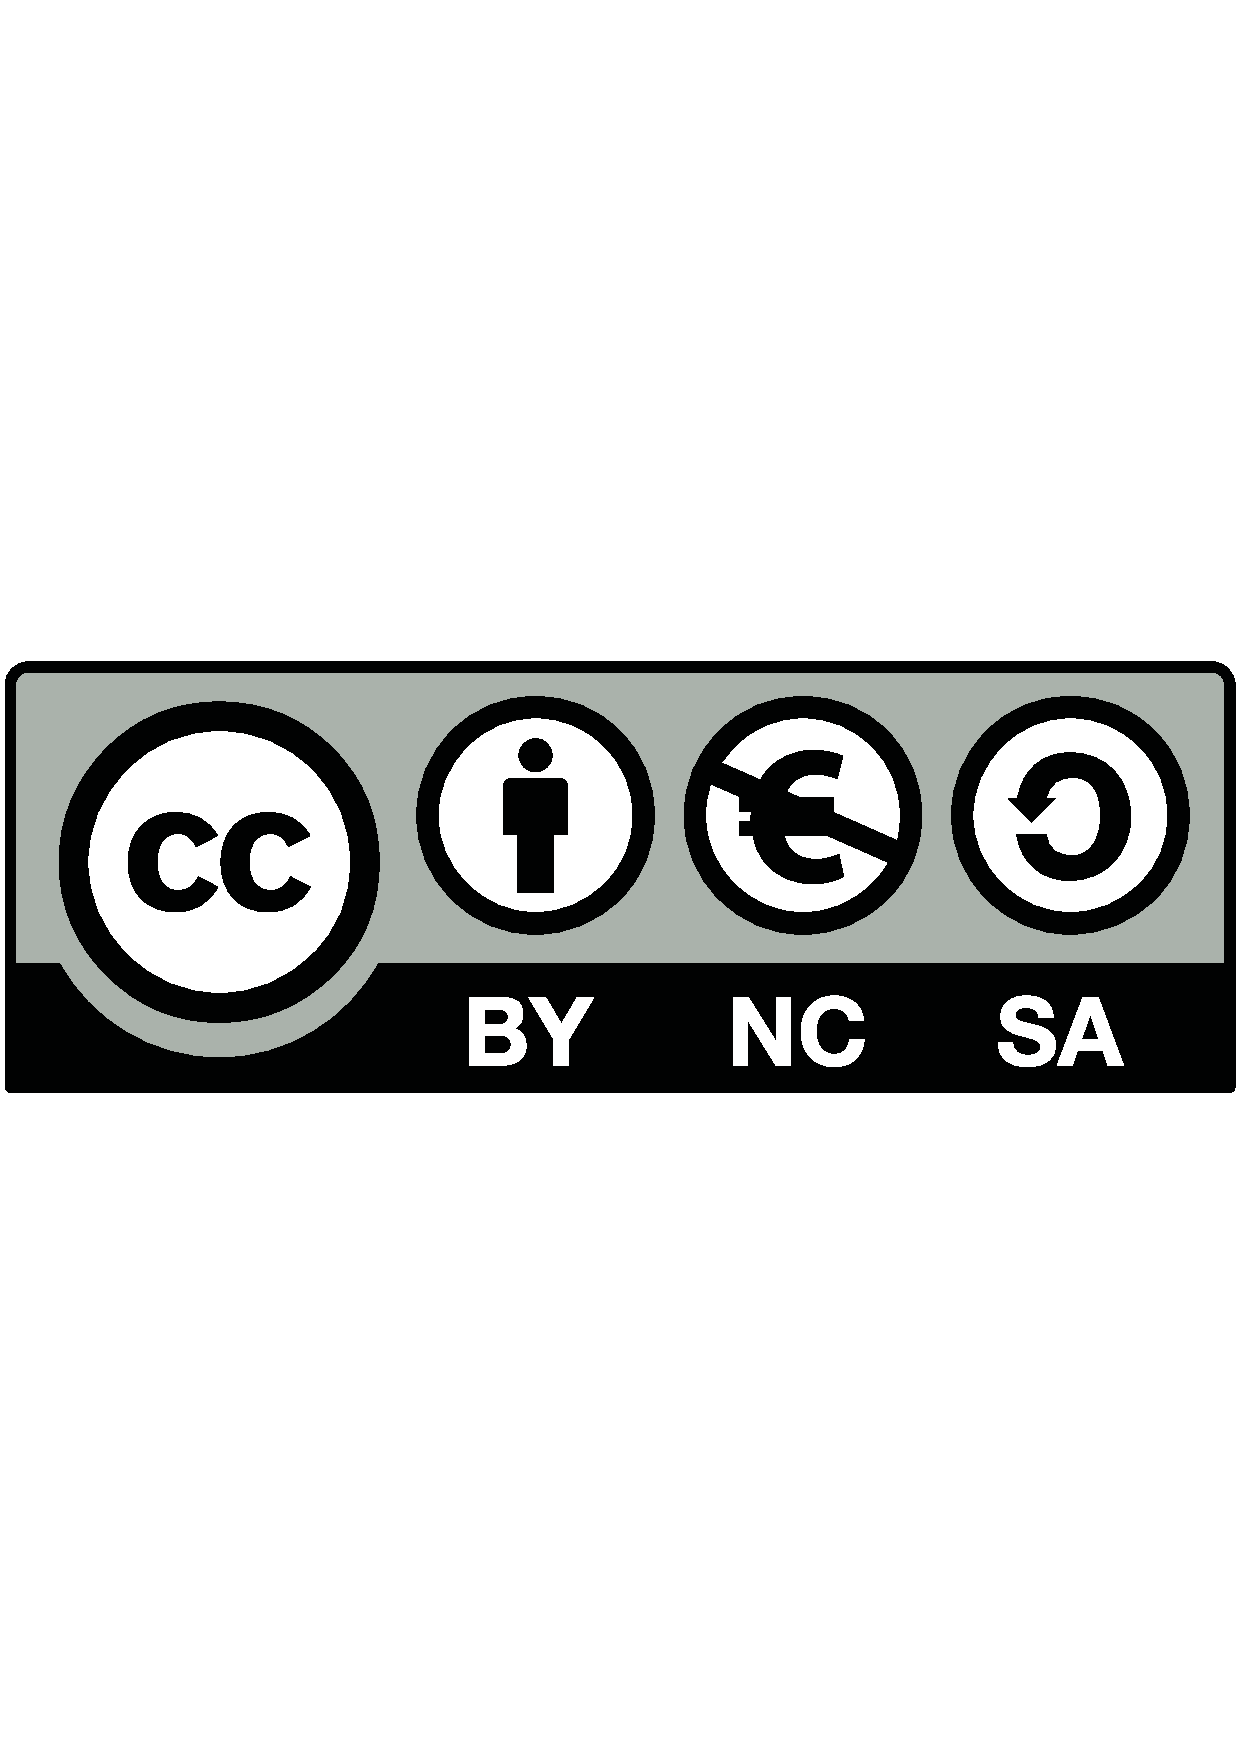
\includegraphics[scale=0.1]{by-nc-sa} \\
        %\scshape \noindent \small \copyright \ \small Diego Duque Zumajo, 
        %2019 \\
        %This work is licensed under a Creative Commons
        %Attribution-NonCommercial-ShareAlike 4.0 International \\
        %(CC BY-NC-SA 4.0) License.
        %\end{center}
        %\newpage
        %\rm
        }

\begin{document}
\setlength{\epigraphwidth}{0.5\textwidth}


\maketitle
\copyrightpage
\newpage
\pagenumbering{Roman} % para comenzar la numeracion de paginas en numeros romanos

\chapter*{Acknowledgments} % si no queremos que añada la palabra "Capitulo"
\pagestyle{noHeader}  %define page style for the chapters
%\addcontentsline{toc}{chapter}{Agradecimientos} % si queremos que aparezca en el índice
%\markboth{Acknowledgments}{Acknowledgments} % encabezado 

\pagestyle{Contents}  %define page style for the index
\tableofcontents % indice de contenidos

\chapter*{Abstract} % si no queremos que añada la palabra "Capitulo"
%\addcontentsline{toc}{section}{Abstract} % si queremos que aparezca en el índice
\pagestyle{noHeader}  %define page style for the chapters
\markboth{Abstract}{Abstract} % encabezado
blablabla

\chapter*{Resumen} % si no queremos que añada la palabra "Capitulo"
%\addcontentsline{toc}{section}{Resumen} % si queremos que aparezca en el índice
\markboth{Resumen}{Resumen} % encabezado
Esta tesis doctoral estudia el comportamiento de un fluido en contacto con un sólido a nivel nanoscópico. Derivaremos las ecuaciones de movimiento de un fluido que se encuentra en contacto con una esfera sólida de grandes dimensiones (de tal manera que la superficie de la esfera pueda ser aproximada a una pared) empleando la Teoría del \textit{Coarse-Graining} (ToCG). Para ello emplearemos la técnica de los operadores de proyección de Kawasaki-Gunton y supondremos un comportamiento Markoviano para obtener un conjunto de ecuaciones sin términos de memoria. 
Abordaremos el problema del \textit{plateau} que sufren las formulas de Green-Kubo presentes en los coeficientes de transporte de las ecuaciones de movimiento del fluido, ofrenciendo una expresión alternativa sin el problema del \textit{plateau}.  

Para validar la teoría y poder medir los coeficientes de transporte mediante simulaciones de dinámica molecular, derivaremos de nuevo las ecuaciones de la nanohidrodinámica a partir de unas variables hidrodinámicas discretas. 
Para ello dividiremos el sistema a lo largo del eje perpendicular a la superficie de la paredes en una serie de láminas o celdas rectangulares de un grosor determinado separadas por planos nodales, de tal manera que las variables puedan ser definidas en dichas celdas o planos nodales.  
Con el fin de verificar que la derivación es correcta, mostraremos que la ecuaciones obtenidas pueden ser interpretadas como una discretización de las ecuaciones continuas mediante el método de Petrov-Galerkin de elementos finitos.  

La hipótesis de markovianidad es la única aproximación realizada para derivar las ecuaciones de la hidrodinámica. Para validarla emplearemos la teoría de Mori que nos da una expresión de la evolución temporal de las correleaciones de las variables relevantes del sistema. La hipótesis Markoviana es válida siempre y cuando las correlaciones decaigan de forma exponencial. Esto ocurre para celdas suficientemente anchas pero no para celdas estrechas. 

Abordaremos el problema de la markovianidad estudiando el caso más sencillo posible, que es un fluido en condiciones de contorno periódicas. Realizaremos simulaciones de dinámica molecular de un fluido no confinado en las cuales iremos monitorizando las variables relevantes del sistema con el fin de calcular sus correlaciones temporales. 
Observaremos que para el estudio de la markovianidad será conveniente trasladarse al espacio recíproco (en el caso de un fluido en condiciones de contorno periódicas se trata del espacio de Fourier) y comprobar si los modos de la matriz de correlaciones decaen o no de forma exponencial. 

Tras establecer la metodología adecuada para tratar el problema, realizaremos simulaciones de dinámica molecular de un fluido confinado entre dos paredes sólidas. Descubriremos que para una anchura de celda del orden de la distancia molecular, la hipótesis de markovianidad no se cumple para los modos cercanos a la pared. Sin embargo, para celdas más anchas, la hipótesis es validada a expensas de perder efectos de \textit{layering}. 

Mediremos la condición de contorno de \textit{slip} a partir de una definición microscópica de la longitud de \textit{slip} y de la posición hidrodinámica de la pared atómica. Comprobaremos que la expresión obtenida es la dada por Bocquet y Barrat \cite{Bocquet1994} y demostraremos que el coeficiente de fricción es una propiedad intrínseca de la superficie puesto que la distancia de \textit{slip} no depende del tamaño del canal empleado. 


\chapter*{Notation, conventions and quotes}

Functions of microstates $z$ in phase space are denoted with a hat as in $\hat{A}(z)$. We follow this convention except for probability densities, as in $\rho_t(z)$. Operators are denoted with ${\cal CALIGRAPHIC}$ symbols. Vectors and matrices are denoted with {\bf boldfaces}.

Although we will notice when we use it, we follow Einstein summation convention in which, for example the product of two matrices in components is written as
\begin{align}
    (AB)_{\mu\nu} = A_{\mu\nu}B_{\nu\sigma}=\sum_{\nu}A_{\mu\nu}B_{\nu\sigma} \nonumber
\end{align}
%The derivative of a composite function is expressed as
%\begin{align}
%    \frac{\partial}{\partial x}F(g(x))=\frac{\partial F}{\partial g}(g(x))\frac{\partial g}{\partial x}(x) \nonumber
%\end{align}

--------------

The quotes in the beginning of each chapter are taken from books I read over the time I have spent working in this dissertation, the last four years. I have respected the language in which the writter wrote the book. 

%-----------------------------------------------------------------
%INTRODUCTION
%-----------------------------------------------------------------
\setcounter{chapter}{-1}
\chapter{Introduction}
\label{Introduction}
\pagenumbering{arabic}
\pagestyle{chapters}  %define page style for the chapters
\markboth{Introduction}{}
%\epigraph{\textit{Falta cita.}}{Libro \\ AUTOR} 

It was in the December of 1959 when Richard Feynman gave a lecture at the annual American Physical Society meeting at Caltech with the name {\it There's Plenty of Room at the bottom: An Invitation to Enter a New Field of Physics} \cite{Feynman1960}. 
Although there is not unanimity in the scientific community about the real impact of this lecture in the development of the nanotechnology \cite{Nature2009}, it is considered its date of birth \cite{Tourney2008}. 
In the lecture Feynman expresses his intuitive ideas about the world of opportunities that exists when one descents to the micro and nanoscale. 

Seven years later, in 1966, Richard Fleischer directed the science fiction film {\it Fantastic voyage}, based on an original idea of Otto Klement and Jerome Bixby. 
Six month before the release of the film, Isaac Asimov published the homonymous book \cite{Asimov1966} inspired by the screenplay of the movie.  
In both book and movie, a group of scientists, one American intelligence agent, and a pilot are placed inside a submarine called Proteus before being miniaturized to the size of a microbe ($\sim 0.5 \mu m$). The objetive is to inject Proteus into the body of an important scientist affected by a cloot blood in his brain that no traditional surgery can remove. The group will have only one hour before the effect of the miniaturization passes.  

As well as in other areas, the reality outdoes fiction. 
Nanothecnology applied to medical devices is a reality. In the last 20 years there has been a rapidly increase in the nanotechnology patents \cite{Zheng2014} and there is a huge interest in the development of new nanomaterials to treat and diagnose cancer \cite{Nazir2014, Dreaden2012, Kievit2011}. 

%Del paper planar
This   advances  in   miniaturization  and   the  development   of  new
experimental techniques have  increased the
interest in the  theoretical understanding of the  behaviour of fluids in the nano \cite{Bocquet2010,KarniadakisBook2005} and micro \cite{Lauga2005, Bocquet2011,KarniadakisBook2005} scales because at nanoscales  the structure  of the  fluid starts to play an  important
role.   

The
nanoscale can be studied with Molecular Dynamics (MD) simulations and there
is  a wealth  of literature  addressing the  behaviour of  fluids near
walls  with  MD \cite{Koplik1995,Wang2017}.   
The standard  description of structured fluids is  based on the
(classic) Density Functional Theory (DFT) \cite{Evans1979}, with the density
functional   capturing  all   the  relevant   information  about   the
\textit{equilibrium} state  of the fluid.   In recent years,  there has
been a  great interest in  obtaining \textit{dynamic} versions  of the
DFT (DDFT) that would allow one  to discuss not
only equilibrium structured fluids and its correlations but also their
dynamic  behaviour \cite{Lowen2003,Evans2016}.   Since the  pioneering
work by Marconi and Tarazona  \cite{Marconi2000} for Brownian dynamics, several approaches
have been considered  for the formulation of DDFT,
ranging from  kinetic theory  \cite{Guo2006}, to  projection operators
\cite{Espanol2009a},  and variational  approaches \cite{Schmidt20xz}.
Most    existing    works     deal    with    colloidal    suspensions
\cite{Goddard2012,Evans2016}. However, there exist  still a gap in the
treatment  of the dynamics of \textit{simple}  fluids \textit{near  solids} at  scales
where  the  structure  of  the  fluid  is  relevant.   
%In  Ref.   \cite{Espanol2009d}  we   have  formulated  DDFT  based  on
%projection operator  techniques, where the  density field is  the only
%relevant variable.  This is appropriate for colloidal systems that are
%suspended in  a solvent acting as  a thermal bath.  In  that case, the
%density field should  be rather understood as  the concentration field
%which,  being  conserved, is  expected  to  be  a slow  variable.   By
%selecting  the density  field as  the only  relevant variable,  we are
%implicitly assuming that the density  evolves in timescales which are
%much larger than  the timescales corresponding to  other variables in
%the system.  In contrast to  colloidal systems, simple fluids have the
%momentum density and energy density  as conserved variables, and these
%variables may  evolve in  comparable timescales  as the  density.  We
%have  recently extended  DDFT  to {\em  non-isothermal} situations  by
%including the energy density  field \cite{Anero20xz}.  Recent attempts
%in that direction  have also been taken  by Schmidt \cite{Schmidt2011}
%and Wittkowski et al.  \cite{Wittkowski2012}.  The resulting theory is
%valid  for \textit{quiescent}  fluids  or solids  in which  convective
%motion is not present.  In the  present work, we consider the mass and
%momentum density fields of a fluid, allowing to address moving fluids,
%but  we do  not  consider energy  transfer. This  is,  we assume  that
%momentum transfer is  not affected by energy fluxes. This  is the case
%in isothermal  processes or even under  slight temperature differences
%whenever the adiabatic coefficient is  close to one, as corresponds to
%a practically  incompressible liquid  like water at  room temperature.
%The  natural thermodynamic  potential is  the free  energy functional,
%instead   of   an   entropy   functional   as   introduced   in   Ref.
%\cite{Anero20xz}. 
%\\\Note{Fin paper theory}
In  particular,  two phenomena  are
observed near  walls at the  nanoscale.  First, the appearance  of the
density  layering  capturing the  excluded  volume  effects of  single
molecules.   For equilibrium  liquids near  walls, 
DFT has  been an exceptionally good theoretical  tool for the
prediction of  these layering effects \cite{Hansen20xz}.   Second, the
observation that the velocity of fluids  may be nonzero near the wall
surface.
%showing  that  the   no-slip  boundary  condition  does  not
%necessarily holds at the nanoscale.
A quite remarkable  assumption in macroscopic hydrodynamics  is the no
slip boundary  condition that  states that the  velocity of  the fluid
vanishes  at the  surface of  fixed solid  walls \cite{Batcherlor1967}.
This assumption gives the correct predictions for macroscopic flows of
Newtonian  fluids.  However,  as the  length scale  of observation  is
reduced  toward   the  micro  and   nanoscale,  a  large   number  of
experimental   \cite{Lauga2005}   and  computer   simulation   studies
\cite{Koplik1995} has shown that the fluid may actually slip along the
container walls  \cite{KarniadakisBook2005}.  The  first consideration
of this possibility was made  by Navier \cite{Navier1827}, who proposed
a  boundary condition  in  which the  shear stress  is  balanced by  a
friction due  to the wall on  the fluid, leading to  the slip boundary
condition.  To  fix ideas, consider a  planar wall at rest  in contact
with  a flowing  fluid  in a  steady  state.  If  there  is some  slip
velocity $  v_{\rm slip}$ at the  wall then the friction  force on the
wall is assumed to be of the form
\begin{align}
  F^x=-\gamma v_{\rm slip}
\end{align}
The average force  $F^x$ is the total tangential force  exerted by the
wall on  the liquid (equal and  opposite to the force  that the liquid
exerts   on  the   wall).    The   interfacial  friction   coefficient
$\gamma$ is a phenomenological transport coefficient.  The
force $F^x$, in  turn, is due to the tangential  viscous stress due to
the fluid  $F^x=-\eta \frac{\partial  v}{\partial z}$, where  $\eta$ is
the shear  viscosity of the fluid.  From the combination of  these two
equations we obtain the Navier slip boundary condition
\begin{align}
  \delta  \frac{\partial v}{\partial z}=v_{\rm slip}
\label{slipBC}
\end{align}
where the slip length  is defined as
\begin{align}
  \delta=\eta/\gamma
\end{align}
The slip boundary condition (\ref{slipBC}) relates the gradient of the
velocity field with the velocity  field, both evaluated at the surface
of  the solid.   This  phenomenological equation  introduces both  the
viscosity and the friction coefficient as parameters to be fitted from
experiments. 

Of course,  one would  like to find  microscopic expressions  for both
coefficients that would  allow to compute in  advance these parameters
for the specific fluid and wall  interaction of the system.  The first
calculation from first principles  of the friction coefficient between
a fluid and a solid wall was  undertaken by Bocquet and Barrat in 1994
\cite{Bocquet1994}. These  authors used
linear  response  theory   in   order  to  derive  a  Green-Kubo
expression  for the  slip length.   Later  on, the  same authors  
revisited the problem and offered an argument based on the generalized
Langevin  equation  (GLE), leading  to  the  same expression  obtained
earlier\cite{Bocquet20xz}.  Bocquet and Barrat proposed the following  expression for
the friction coefficient
\begin{align}
  \gamma=\frac{1}{Sk_BT}\int_0^{\tau} dt \llangle \hat{F}^x(t)\hat{F}^x\rrangle
\label{lambdawall}
\end{align}
in terms of  the equilibrium autocorrelation function  of the parallel
component of the microscopic fluctuating force $\hat{F}^x(t)$ that the
liquid exerts on  a planar wall of area  $S$.  equation  (\ref{lambdawall})
represents  an  important step  in  offering  a statistical  mechanics
foundation  of  a boundary  condition,  with  a caveat:  the  friction
coefficient as a  function of the upper limit of  integration does not
have a plateau  and it decays to zero for  large $\tau$. 
However, the
formula is still useful when one expresses the force-force correlation
in terms of density-density correlations,  which are then treated with
the well-known hydrodynamic theory of fluctuations.  In that case, the
hydrodynamic  exponential   decay  assumed  for   the  density-density
correlation makes  the integral  non-vanishing and  allows one  to get
explicit     analytical    estimates     for    the     slip    length
\cite{Barrat1999,Bocquet2007,Kobryn2008,Kobryn2011}.

The  validity of  the Bocquet and Barrat approach has  been a  subject of  an ongoing
debate  \cite{Petravic2007,Hansen2011,Huang2014} that  we believe  has
not yet  been concluded (see  the recent  account of the  situation of
this  debate  by   Ramos-Alvaro  et  al.   \cite{Ramos-Alvarado2016}).
Petravic and Harrowell \cite{Petravic2007}  argued that the Green-Kubo
expression given by Bocquet and Barrat is not  an intrinsic property of the surface of
solid-liquid interaction  but rather  contains also  information about
the bulk friction between two  parallel plates.  It was further argued
that  the Bocquet and Barrat Green-Kubo formula  gives, in  fact, the  friction force
between two parallel  plates with a liquid in  between and, therefore,
depends  on the  separation  between  the plates.   In  this way,  the
transport coefficient  (\ref{lambdawall}) would not be  an interfacial
friction coefficient  tied to interfacial properties  alone.  Petravic
and Harrowell conclude ``that  the Navier friction coefficient cannot,
in  general,  be obtained  from  the  surface force  time  correlation
function  alone  since  these   fluctuations  are  coupled  to  stress
fluctuation  throughout  the  entire  system''.   While  Petravic  and
Harrowell present an  indirect Green-Kubo expression for the  slip length (for
the case of identical parallel walls), the problem was reconsidered by
Hansen, Todd,  Davis \cite{Hansen2011} by  looking at a  GLE involving
the force on a fluid slab of  width $\Delta$ near the wall and relating
it with  the center of  mass velocity of  the slab through  a friction
coefficient (a memory  kernel in a non-steady state  in general).  The
method is  extended to cylindrical geometries  also \cite{Kannam2012}.
By running equilibrium molecular dynamics (MD) simulations one can get
the friction coefficient and the  slip length throught the correlation
functions of the  variables involved.  Hansen et al. propose  a GLE of
the form
\begin{align}
  F'^x(t)=-\int_0^t \zeta(t-\tau)u_{\rm slab}(\tau)d\tau+F'_r(t)
\label{Hansen1}\end{align}
where $ F'^x(t)$ is the force that the solid exerts on the fluid slab,
$u_{\rm slab}$  is the velocity  of the slab  (the wall is  assumed at
rest  here), $\zeta(t-\tau)$  is a  memory kernel  and $F'_r(t)$  is a
random  force.   For a steady  state,  one  obtains the  average  result
$\llangle F'^x\rrangle=-\zeta_0 \llangle  u_{\rm slab}\rrangle$, where
$\zeta_0$  is  the zero  frequency  friction  coefficient which  is  a
parameter  that  can  be  explicitly measured  in  MD  simulations  by
comparing  correlations  inferred  from  (\ref{Hansen1}).  By  solving
Navier-Stokes equations  with integral boundary conditions,  Hansen et
al.   obtain  an  explicit  form  for the  slip  length  in  terms  of
$\zeta_0$. This coefficient is shown to be independent on channel width
and, therefore, it is an intrinsic surface property, as expected for
the interfacial friction coefficient.

More recently,  Huang and  Szlufraska propose  an \textit{alternative}
definition of a friction  coefficient\cite{Huang2014}. In this case, a
GLE  for   the  velocity  of  a  \textit{single liquid  particle}  is
constructed with the Mori  projection operator.  While comparisons are
made with the Bocquet and Barrat expression,  claiming superior performance, the truth
is that no  connection between the obtained friction  coefficient of a
single particle and the slip length is made in Ref.  \cite{Huang2014}.
The  single particle  friction coefficient,  while interesting  by its
own, does  not inform us  about the parameter  that is crucial  in the
boundary condition, which  is the slip length.   However, Bhadauria et
al. \cite{Bhadauria2015} have used  the model in Ref. \cite{Huang2014}
in order to  study parallel flow of  water in a confined  slit made of
graphene and silico.  It is obvious  that what it is called ``friction
coefficient'' depends  very much on  the variables that  are connected
with  the  force  on the  wall  due  to  the  fluid, be  the  velocity
difference between  parallel walls\cite{Bocquet1994,Petravic2007}, the
velocity of a fluid slab\cite{Hansen2011}, or the velocity of a single
particle of the fluid\cite{Huang2014}.


Recently, Chen  et al. have  revisited the  problem of looking  at the
hydrodynamic modes of a channel between parallel walls\cite{Chen2015}.
By   comparing  results   of   MD  simulations   and  predictions   of
hydrodynamics they were  able to locate the plane of  slip, as well as
measuring the slip length in the problem as in \cite{Bocquet1994}.  In
addition,  they  formulated a  Green-Kubo  expression  for both,  bulk
viscosity and interfacial  friction coefficient that, in  the limit of
very wide channels coincides with  Bocquet and Barrat expression.  The size dependence
of the Bocquet and Barrat Green-Kubo expression dissappears in this limit.

In summary, there  seems to be three different ways  of looking at the
derivation  of  the  slip   boundary  condition  from  Non equationilibrium
Statistical Mechanics (NESM): 
\begin{enumerate}
  \item Through the  measurement of the correlation of
the  transverse  momentum  and  comparison  with  the  predictions  of
continuum  (local) hydrodynamics  \cite{Bocquet1993,Chen2015}.
\item Through
linear  response theory  relating  the  force on  the  walls with  the
velocity   of  the   fluid   \cite{Bocquet1993,Petravic2007}.
\item By
formulating  linear,  in  general  non-Markovian,  conections  between
friction forces and velocities \cite{Hansen2011}, where the meaning of
this quantities is often understood implicitly.
\end{enumerate}

Given this mess in the derivation of the slip boundary condition, in this dissertation address the slip problem from first principles. Following the work by Robertson \cite{Robertson1966} and Piccirelli \cite{Piccirelli1968}, who derived the hydrodynamic equations from the microscopic dynamics of a fluid, we obtain a set of continuum equations which describe the behaviour of a fluid in contact with a solid with the Markovian approximation as the only assumption. 
Because the validation of the theory is only possible through MD simulations, we derive the discrete equations with the same methodology as in continuum theory. 
A cross-check is given using a Petrov-Galerkin  finite element discretization method in order to obtain from the continuum equations the resulting discrete equations previously derived.  
Once we have the discrete equations, we address the study of the markovian behaviour of the simplest case (i.e. a fluid in periodic boundary conditions). We restrict the study to planar dynamics monitoring only the transverse momentum component. We use the same methodology to study the markovian behaviour of a confined fluid between two parallel solid slabs and we show how the marovian approximation is only valid when the size of the bin is bigger than the molecular length. Finally, we measure the transport coefficients that appear in the hydrodynamic equations in order to validate the theory. 
After that, the slip boundary condition is measured from a microscopic definition of the slip length and the position of the atomic wall.
In contrast with the conclussion of Petravic and Harrowell \cite{Petravic2007}, we obtain, as Bocquet and Barrat \cite{Bocquet1994}, that the slip length is an intrinsic surface property. That means that it does not depend on the geometry of the channel. 

This dissertation is structured as follows. 
In the first chapter we review NESM in order to state the foundations in which the following chapters are based. 
We introduce two projection operator that allows us to obtain hydrodynamic equations: the Kawasaki-Gunton projector \cite{Kawasaki1973} and the Mori projector \cite{Mori1965}.  The first one allows one to obtain  nonlinear closed equations
for  the  averages  of   the  selected  variables of the system, while under the Mori theory one obtains simple equations not only for the averages of the relevant variables, but also for their correlation functions. 

In the second chapter, we derive the hydrodynamic equations of a fluid in contact with a solid. In order to discuss total momentum conservation we choose a macroscopic solid sphere. 
To do so, we derive DDFT for a simple fluid including the mass and the momentum density field.
We use the Kawasaki-Gunton operator technique to obtain the equations of motion of the time dependent average of these fields assuming the Markovian aproximation. 
The resulting equations contain transport coefficients given by  Green-Kubo formulas, which suffer from the plateau problem when the separation of timescales is not large.  
This well-known problem arises because the Green-Kubo running integral appearing in the expressions of the tranport coefficients decays as the correlation of the selected coarse-grained (CG) variables when the projected dynamics is approximated by the unprojected Hamiltons dynamics. 

The third chapter is a derivation from macrocopic principles of the discrete equations of hydrodynamics in the presence of a planar wall. 
We bin the system in slabs as is shown in Figure \ref{fig:WallsBox1}. The yellow lanes are called {\it nodes} and they separated the {\it bins} in which the system is binned. We start from a discrete mass and momentum densities fields defined in the nodal planes in order to derive the hydrodynamic equations with the Kawasaki-Gunton projector. Also we validate the final discrete equations  with a discretization of the continumm hydrodynamic equations using the Petrov-Galerkin finite element discretization method.   
The main objetive of this chapter is to obtain the discrete transport coefficients in order to compute them with MD simulations. 
\begin{figure}
    \centering
    %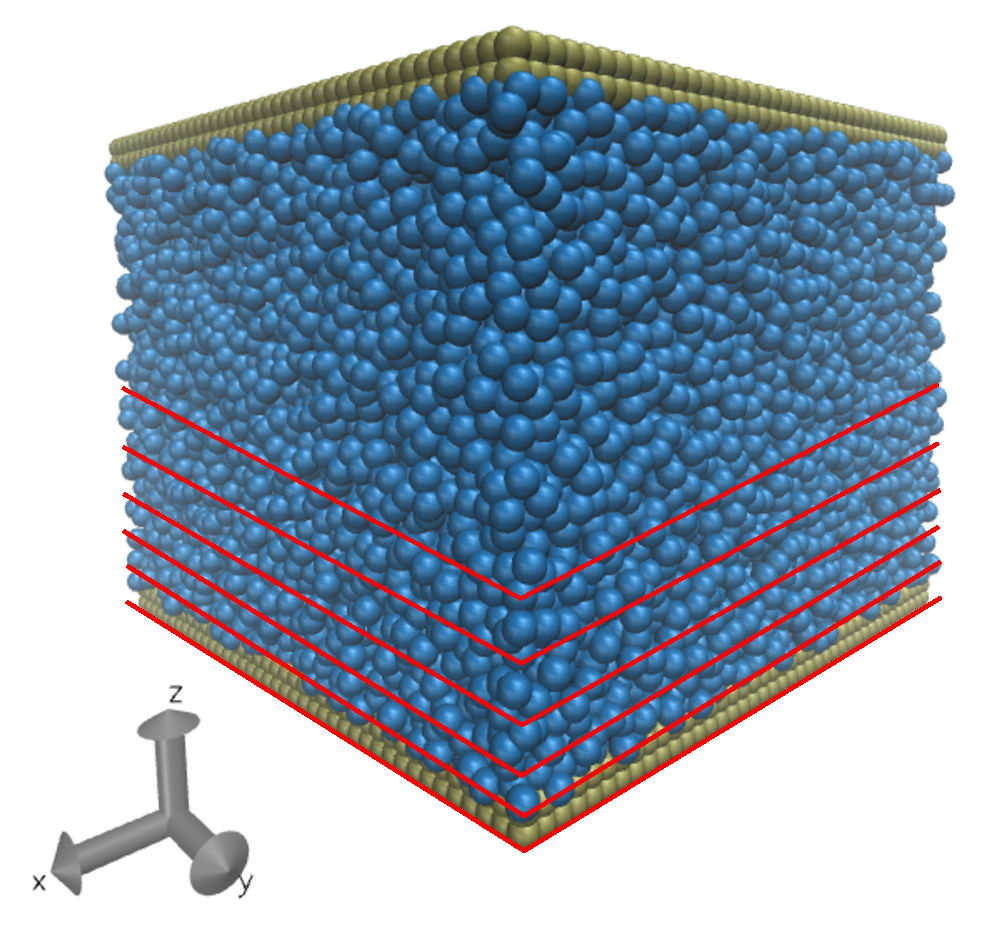
\includegraphics[scale=0.3]{system_nodes_walls}
    \frame{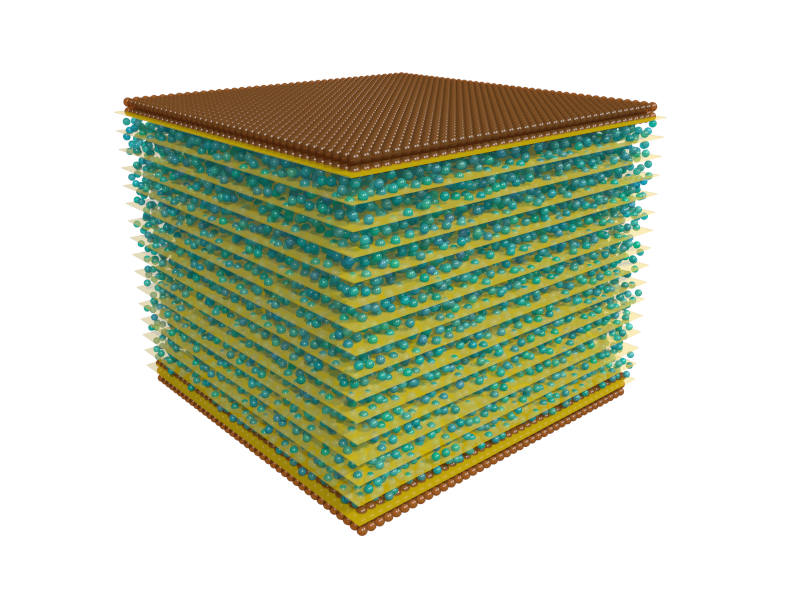
\includegraphics[width=.5\linewidth]{PRL3_gold2_wo_diffuse}}
    \caption[Sketch of the binning used]{A visual representation of a MD simulation with a sketch of the binning used. In yellow are depicted the nodal planes used.}
    \label{fig:WallsBox1}
\end{figure}

In the first part of the fourth chapter the plateau problem is adressed in order to obtain, within Mori projection operator formulation, an alternative expression for the transport coefficients with a corrected Green-Kubo expression with no plateau problem. 
The corrected Green-Kubo expression is crucial for this dissertation because the results of the chapters \ref{Chap:PBC}, \ref{Chap:Walls} and \ref{Chap:Slip} are based on this new corrected Green-Kubo expresion. 

In the second part of this chapter the correlation matrix of the discrete transverse momentum density field is studied through MD simulations in order to determine to what extent the Markovian approximation is valid with a nonlocal space description of hydrodynamics. 
The goal is to understand a simpler case before moving to a system more complicated such as a fluid confined between two solid walls. 
One important learning about this chapter is that we have to consider to the reciprocal space (i.e. the Fourier space in the case of unconfined systems) to discuss unambiguously the Markov property.
The method followed in this chapter will be extrapolated to the study of  confined fluids. 

In Chapter \ref{Chap:Walls} MD simulations are performed to compute the correlation matrix of the discrete transverse momentum density field of a fluid between two solid slabs. 
Because the objetive of this chapter is to study the effect of the size of the bin on the Markovian behaviour near the solid walls, the system is discretized using two size of the bins. We realize that for bins smaller than the molecular size the description near the walls can not be Markovian, while for larger bins the description can be deemed Markovian.  

Finally, in the last chapter  the nonlocal transport kernels that appear in the discrete theory presented in the third chapter are measured through MD simulations. 
We use the corrected Green-Kubo expression in order to avoid the plateu problem. 
The main result of this chapter is the calculation of the slip length and the location of the hydrodynamic position of the atomic wall. We conclude that the slip lenght does not depend on the size of the channel and, therefore, it is a intrinsic surface property.  


%\section{Objetives reached in this dissertation}
%This dissertation consist on six publications sorted by the chronological order of publications, which is, in fact, the logical order. 
%
%The objetive of the first publication, {\it Nanoscale hydrodynamics near solids}, is to derive the hydrodynamic equations of a fluid in contact with a solid. 
%In order to reach it, we derive Dynamic Density Functional Theory (DDFT) for a simple fluid including the mass and the momentum density field.
%We use the Kawasaki-Gunton operator technique to derive the equations of motion of the time dependent average of these fields assuming the Markovian aproximation. 
%The resulting equations contain transport coefficients given by  Green-Kubo formulas, which suffer from the plateau problem when the separation of timescales is not large.  
%This well-known problem arises because the Green-Kubo running integral appearing in the expressions of the tranport coefficients decays as the correlation of the selected variables when the projected dynamics is approximatd by the unprojeted Hamiltons dynamics. 
%
%The second publication, {\it Revisiting the plateau problem in the Green-Kubo formula}, adresses the plateau problem in order to obtain, within Mori projection operator formulation, an alternative expression for the transport coefficient with a corrected Green-Kubo expression with no plateau problem. 
%The expression obtained allows us to compute with MD simulations the 
%The corrected Green-Kubo expression derived in this publication is crucial for the dissertation. The results of the chapters \ref{Chap:PBC}, \ref{Chap:Walls} and \ref{Chap:Slip} are based on this new corrected Green-Kubo expresion. 
%
%The third, fourth, fifth and sixth publication were published as a series of discrete hydrodynamics.
%The first publication of the series, {\it Discrete Hydrodynamics I: Theory for planar flows with confinig walls}, is just a discretization of the resulting equations of the first paper. 
%We bin the system in slabs as is shown in Figure \ref{fig:WallsBox}. The red lines are called {\it nodes} and they separated the {\it bins} in which the system is binned. We start from a discrete mass and momentum densities fields defined in the nodal planes in order to derive the hydrodynamic equations with the Kawasaki-Gunton projector. Also we validate the final discrete equations  with a discretization of the continumm hydrodynamic equations using the Petrov-Galerkin finite element discretization method.   
%The final objetive of this publication is to obtain the discrete transport coefficients in order to compute them with MD simulations. 
%\begin{figure}
%    \centering
%    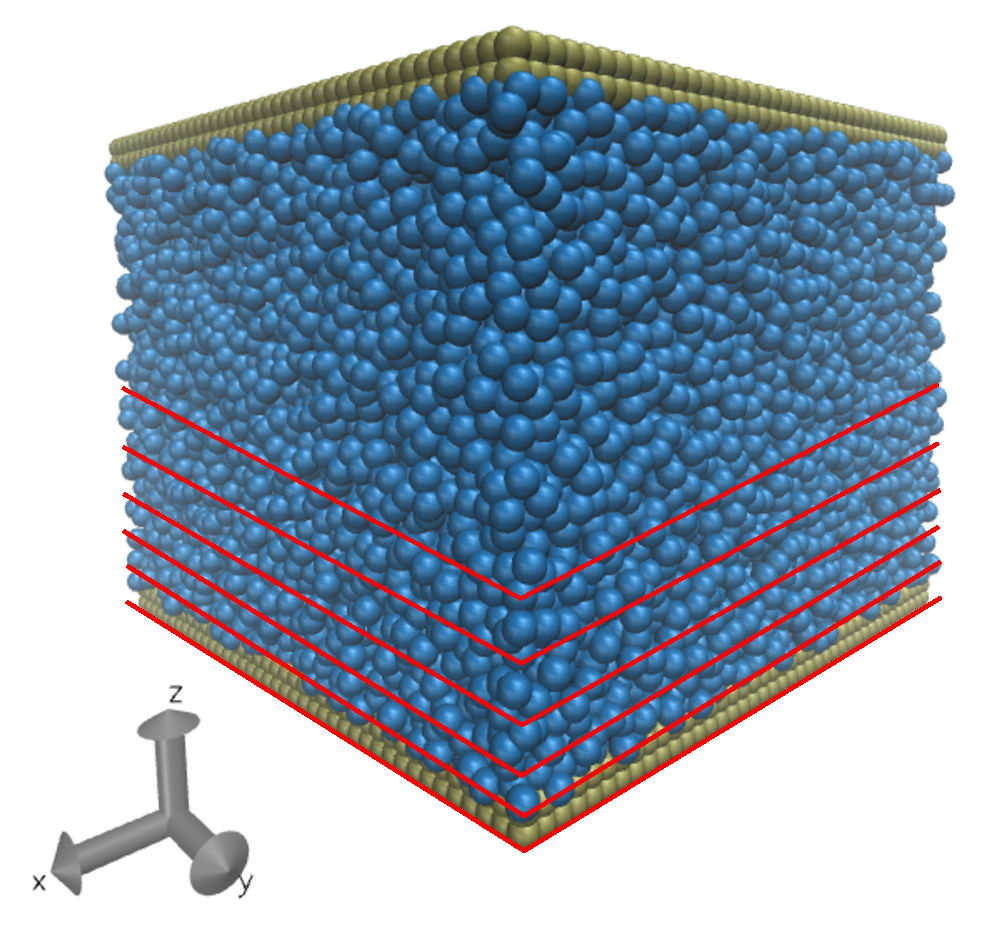
\includegraphics[scale=0.3]{system_nodes_walls}
%    \caption[Walls box]{A visual representation of the MD simulation with a sketch of the binning used. In red are depicted the nodal planes used.}
%    \label{fig:WallsBox}
%\end{figure}
%
%In the second publication of the series, {\it Discrete hydrodynamics II: Space and time locality for unconfined fluids}, we study through MD simulations the correlation matrix of the discrete transverse momentum density field in order to determine to what extent the Markovian approximation is valid with a nonlocal space description of hydrodynamics. The objetive of this publication is to understand a simpler case before moving to a system more complicated such as a fluid confined between to solid walls. 
%One important learning about this publication is that we have to move to the reciprocal space (i.e. the Fourier space in the case of unconfined systems) in order to observe the time from the Markovian approximation is valid. 
%The method followed in this publication will be extrapolated to the study of a confining fluids. 
%
%In the third publication of the series, {\it Discrete hydrodynamics III: Non-Markovian behaviour near solids walls}, we perform MD simulations in order to compute the correlation matrix of the discrete transverse momentum density field of a fluid between two solid slabs. 
%Because the objetive of this publication is to study the effect of the size of the bin on the Markovian behaviour near the solid walls, we discretize the system using two size of the bins. 
%
%Finally, the objetive of the last publication of this series, {\it Discrete hydrodynamics IV: The slip boundary condition}, is to measure through MD simulations the nonlocal transport kernels that appear in the discrete theory presented in the first part of the series. 
%We use the corrected Green-Kubo expression in order to avoid the plateu problem. 
%The main result of this publication is the calculation of the slip length and the location of the hydrodynamic position of the atomic wall. We conclude that the slip lenght does not depend on the size of the channel and, therefore, it is a intrinsic surface property.  
% 



%-----------------------------------------------------------------
%CHAPTER 1
%-----------------------------------------------------------------
\chapter{Nonequilibrium Statistical Mechanics}
\label{Chap:NESM}
\pagestyle{chapters}  %define page style for the chapters
\markboth{Nonequilibrium Statistical Mechanics}{}
\epigraph{\textit{There is no future. There is no past. Do you see? Time is simultaneous, an intricately structured jewel that humans insist on viewing one edge at a time, when the whole design is visible in every facet.}}{Watchmen \\ ALAN MOORE} 
%No hay futuro. No hay pasado ¿Lo ves? El tiempo es simultáneo, una joya de una estructurada demasiado compleja en donde los humanos se empeñan en solo ver un borde, cuando el diseño por completo es visible en todas las facetas.-Alan Moore.

\section{Introduction}
It was in the nineteen century when Statistical Mechanics was born mainly because of the work of Ludwing Boltzmann and Josiah Willard Gibbs. The goal was to reconcile Thermodynamics with the microscopic laws known at that time. 

Thermodynamics was well-established because it draws its concepts from experiments while the attemps to understand it from the Newton's laws collided with problems such as the imposibility of taking into account the interactions between all the particles of a thermodynamic system, the highly nontrivial form of theses interactions, the huge number of degrees of freedom or the Loschmidt's paradox\footnote{The second law of thermodynamics establishes that the entropy of an isolated system increases with time. This can be understood as a time direction imposed by the increasing of the entropy. Furthermore, Newton's laws are reversible. According to Josef Loschmidt this apparently conflict could be the responsible of the imposibility to derive the laws of the thermodynamics from the microscopic laws.}. 
To avoid these problems physicists realized that the macro properties of a thermodynamic system does not strongly depend on the exact dynamics of every particle, but more on the averages that eventually erode the details of the behaviour of the particles. 
Thus, the link between the microscopic and macroscopic theory of matter can be stated through statistical techniques to the microscopical mechanics laws. 
The connection is possible to the notion of \textit{ensemble}, which is a collection of imaginary systems with a set of common macroscopic properties.  

Statistical Mechanics is a theoretical framework which allows one to study the macro-properties of a many-body system from the dynamics of its microcopic constituents.
Therefore, we may roughly say that Statistical Mechanics acts as a bridge between two levels of description: {\it microscopic level} governed by the Newton's laws of motion and the {\it macroscopic level} in which the knowledge is adquired from the experiments.
A beautiful but rough example about how Statistical Mechanics works can be found in the book of Dean Rickles {\it Philosophy of Physics} \cite{Rickles2016}.
He imagines a large musical ensemble playing in concert.
The ``global'' sound produced by the musicians is analogue to the thermodynamic variables obtained from the colisions between the particles in the system. 
The music can me analized from two levels: the global level, where the harmony and the musical form take an important role, and the individual level, in which we focus in what the musicians are playing to produce the global sound. ``Is this zooming in and out'', in words of Rickles, ``from the whole system to its parts, that characterizes the relationship between statistical mechanics and thermodynamics: you won't see harmonies in a single bassoon; likewise, you won't see pressure or temperature in an individual molecule.''

The equilibrium theory of Statistical Mechanics provides an interpretation for the equilibrium thermodynamic systems from a molecular point of view. The models that allow us to reproduce real systems are the well-known microcanonical, canonical, and grand canonical ensembles. These ensembles are idealizations. They does not reproduce exactly real experiments, but give us useful information about them. 
However, most of the phenomena present in the Nature are in nonequilibrium in the timescale of our observation. A nonequilibrium system may be modeled perturbating an equilibrium ensemble that forces the system to not relax to equilibrium.  
Einstein \cite{Einstein1905}, Onsager \cite{Onsager1931} and Kirkwood \cite{Kirkwood1946} made important contributions to NESM years before Green \cite{Green1952, Green1954}, in the fifties, formulated it as we know nowadays. 
It was in the 60's when Zwanzig \cite{Zwanzig1961} and Mori \cite{Mori1965} reformulated the theory using the technique of the projection operators \cite{Grabert1982}. 


\section{Hamilton's equations and the evolution of the microstates}
\label{Sec:Hamilton}
Consider a system consisting of $N$ particles of mass $m$ in a volume $V$. 
In Classical Mechanics the positions of the particles ${\bf q}^N\equiv ({\bf q}_1,\dots,{\bf q}_N)^T$ and their 3N momenta ${\bf p}^N\equiv ({\bf p}_1,\dots,{\bf p}_N)^T$ specify the state of the system at any time. 
The collection of the positions and momenta of the particles defines the microscopic state of the system, $z=(q,p)^T$, which is a {\it phase point} in the {\it phase space} $\Gamma$ of 6N dimensions. 
The notation emphasizes that $z$ is a column vector, where $T$ is the transpose. 
Therefore, the time evolution of a phase point $z_t$ is called the {\it phase trajectory} and it is determined by the Hamilton's equations of motion
%
\begin{align}
  \dot{{\bf q}}_i = \frac{\partial \hat{H}}{\partial {\bf p}_i}&,& \dot{{\bf p}}_i = -\frac{\partial \hat{H}}{\partial {\bf q}_i}
  \label{Hamiltonequation}
\end{align}
%
Typically the Hamiltonian has the form
%
\begin{align}
    \hat{H}(z) = \sum_{i=1}^{N}\frac{{\bf p}_i^2}{2m}+\hat{U}({\bf q}_1,\dots,{\bf q}_N)+\sum_{i=1}^{N}\Phi({\bf q}_i),
\end{align}
%
where the first sum is the kinetic energy of the system, the potential of interaction
between particles is $\hat{U}({\bf q}_1,\dots,{\bf q}_N)$ and $\Phi({\bf r})$ is a time-independent external potential. 

%Note that the the phase trajectories can not pass through the same point of the phase space because the evolution of the phase point is subject to 6N initial conditions. 
%Thus, if two trajectories in phase space cross is because they started at the same phase point.  

Hamilton's equations can be written in compact form as
%
\begin{align}
  \dot{z}_t = J\cdot\frac{\partial\hat{H}}{\partial{z}}(z_t)\equiv \hat{v}(z_t),
  \label{compactHamiltonEq}
\end{align}
%
where we have defined the Hamiltonian vector field $\hat{v}(z_t)$ and $J$ is the symplectic matrix\footnote{J is an orthogonal matrix, $J^TJ=1\to J^T = J^{-1}$, and its square is the minus the identity matrix $J^2=-1$} with the form
$$
\begin{pmatrix} 
  0 & +1_{3N} \\
  -1_{3N} & 0 
\end{pmatrix},
$$
where $1_{3N}$ is the identity matrix of dimension $3N \times 3N$.

Hamilton's equation (\ref{compactHamiltonEq}) indicates that the trajectory of $z_t$ in phase space is an integral curve of the velocity field. Therefore, if we follow the direction given by the velocity field we can figure out which microstate will be the next one. 


\subsection{Hamilton's equations in operator form}
Hamilton's equations are in general a {\it set of nonlinear ordinary differential equations}. However, in the language of linear operators we may obtain linear equations that are amenable of theoretical treatment. 

%By analogy with Quantum Mechanics (QM) we consider all functions $\hat{B}(z)$ in phase space as a Hilbert vector space. 
%Each function $\hat{B}(z)$ is a vector in the infinite-dimensional Hilbert space vector. 
%As well as the state vector in QM, $|\Psi\rangle$, each function (vector) $\hat{B}$ has the dimension of all the possible microstates in which the system might be. 
We consider all functions $hat{B}(z)$ in phase space as vectors in infinite-dimensional vector space. 
The identity function in phase space is denoted as $\hat{z}$. It takes any microstate $z$ into $\hat{z}(z)=z$. 
We carefuly distinguish the argument $z$, which is a point in the phase space, from the vector of the Hilbert space $\hat{z}$, which represents the identity function.

The Liouville operator $i{\cal L}$ is an important operator in the dynamics of the microstatates. It has the following explicit form 
\begin{equation}
    i{\cal L} = -
    \sum_i\left[\frac{\partial \hat{H}}{\partial {\bf q}_i}
\frac{\partial    }{\partial {\bf p}_i}-
\frac{\partial \hat{H}}{\partial {\bf p}_i}
\frac{\partial }{\partial {\bf q}_i}\right]
\label{iL}
\end{equation}
In order to give a more compact form of the action of the Liouville operator on a phase function we introduce the {\it Poisson bracket}
\begin{align}
  \{\hat{A},\hat{B}\}\equiv\left(\frac{\partial\hat{A}}{\partial z}\right)^T\cdot J\cdot\frac{\partial\hat{B}}{\partial z}= 
  \sum_i\left[\frac{\partial \hat{A}}{\partial {\bf q}_i}
    \frac{\partial \hat{B}}{\partial {\bf p}_i}-          
    \frac{\partial \hat{A}}{\partial {\bf p}_i}
  \frac{\partial\hat{B} }{\partial {\bf q}_i}\right]
    \label{PoissonBracket}
\end{align}
%\begin{align}
%  \{\hat{A},\hat{B}\}\equiv\left(\frac{\partial\hat{A}}{\partial z}\right)^T\cdot J\cdot\frac{\partial\hat{B}}{\partial z}= 
%  \sum_i\left[\frac{\partial \hat{A}}{\partial {\bf q}_i}
%    \frac{\partial \hat{B}}{\partial {\bf p}_i}-          
%    \frac{\partial \hat{A}}{\partial {\bf p}_i}
%  \frac{\partial\hat{B} }{\partial {\bf q}_i}\right]
%    \label{PoissonBracket}
%\end{align}
Therefore, taking an arbitrary phase function $\hat{B}(z)$ the Liouville operator acts on it in this way
%\begin{align}
%  i{\cal L}\hat{B}=-\left(\frac{\partial\hat{H}}{\partial z}\right)^T\cdot J\cdot\frac{\partial\hat{B}}{\partial z}
%  =\hat{v}^T\cdot\frac{\partial\hat{B}}{\partial z}
%  = \frac{\partial^T}{\partial z}\cdot\left(\hat{H}\hat{B}\right) 
%  = -\{\hat{H},\hat{B}\}
%  \label{iLB}
%\end{align}
\begin{equation}
  i{\cal L}\hat{B} 
%  =-    \sum_i\left[\frac{\partial \hat{H}}{\partial {\bf q}_i}
%      \frac{\partial\hat{B}}{\partial {\bf p}_i}-
%\frac{\partial \hat{H}}{\partial {\bf p}_i}
%\frac{\partial\hat{B} }{\partial {\bf q}_i}\right]
%=-\left(\frac{\partial\hat{H}}{\partial z}\right)^T\cdot J\cdot\frac{\partial\hat{B}}{\partial z}
  = -\{\hat{H},\hat{B}\}
\label{iL}
\end{equation}

%Where we have introduce the {\it Poisson bracket} to give a more compact form of the action of the Liouville operator on a phase function. 

%In order to give a more compact form of the action of the Liouville operator on a phase function we have introduced the Poisson bracket
%\begin{align}
%  \{\hat{A},\hat{B}\}\equiv\left(\frac{\partial\hat{A}}{\partial z}\right)^T\cdot J\cdot\frac{\partial\hat{B}}{\partial z}= 
%  \sum_i\left[\frac{\partial \hat{A}}{\partial {\bf q}_i}
%    \frac{\partial \hat{B}}{\partial {\bf p}_i}-          
%    \frac{\partial \hat{A}}{\partial {\bf p}_i}
%  \frac{\partial\hat{B} }{\partial {\bf q}_i}\right]
%    \label{PoissonBracket}
%\end{align}

The action of the Liouville operator on the identity function $\hat{z}$ is
\begin{align}
  i{\cal L} \hat{z} = \hat{v}
  \label{iLz}
\end{align}

Therefore, in the language of the Liouville operator we can transform a complicated nonlinear function $\hat{v}$ into the action of a linear operator $i{\cal L}$ on the identity function $z$.

With the equation (\ref{iLz}) the Hamilton's equations (\ref{compactHamiltonEq}) can be written in terms of the Liouville operator as
\begin{align}
  \frac{d}{dt}z_t=i{\cal L}\hat{z}(z_t)
  \label{Devzt}
\end{align}

In order to obtain an expresion for $z_t$, we consider a Taylor expansion of the trajectory $z_t$ around $t=0$, that is,
\begin{align}
    z_t=z_0+\frac{dz_t}{dt}(0)t+\frac{1}{2!}\frac{d^2z_t}{dt^2}(0)t^2+\cdots
    \label{ztExp}
\end{align}
From (\ref{Devzt}) we have the first order derivative. All the high order time derivatives are given by
%
\begin{align}
    &\frac{d^2z_t}{dt^2} = \frac{d}{dt}i{\cal L}\hat{z}(z_t)
    =\hat{v}^T(z_t)\cdot\frac{\partial i{\cal L}\hat{z}}{\partial z}(z_t)
    =(i{\cal L})^2\hat{z}(z_t) \nonumber \\ 
    &\vdots \nonumber \\ 
    &\frac{d^n z_t}{dt^n} =(i{\cal L})^n\hat{z}(z_t)
\end{align}
%
Evaluating all these time derivatives at $t=0$, the equation (\ref{ztExp}) becomes
\begin{align}
    z_t=\hat{z}(z_0)+i{\cal L}\hat{z}(z_0)t
    +\frac{1}{2!}(i{\cal L}^2)\hat{z}(z_0)
    +\cdots
    ={\rm exp}\{i{\cal L}t\}\hat{z}(z_0),
    \label{zt1}
\end{align}
where the exponential operator can be defined as a Taylor expansion

\begin{align}
  {\rm exp}(i{\cal L}t) \equiv {\cal I} + i{\cal L}t + \frac{1}{2!}(i{\cal L}t)^2 + \frac{1}{3!}(i{\cal L}t)^3 +  \frac{1}{4!}(i{\cal L}t)^4 + \cdots,
\end{align}
where ${\cal I}$ is the identity operator.
The notation of the time evolution equation (\ref{zt1}) is usually simplified in this way 
\begin{align}
  z_t = exp\{i{\cal L}t\}z_0
  \label{zt}
\end{align}
without forgetting that what we are doing is to apply an operator ${\rm exp}\{i{\cal L}t\}$ to a phase function $\hat{z}$, giving as a result ${\rm exp}\{i{\cal L}t\}\hat{z}$, and then evaluate this result at the value $z_0$.


\section{The Liouville theorem}
We have seen that Hamilton's equations (\ref{compactHamiltonEq}) are first order differential equations governing the deterministic evolution of the system. 
These equations need an initial condition $z_0$, which is impossible to know in practice because in general we have not access to the position and momenta of every single particle in the system. Usually, a system is prepared under identical macroscopic conditions that do not allow to fix the value of the initial condition. 
Different configurations of the particles can give an identical macroscopic condition. 
This enforces the introduction of a {\it probability density} $\rho_0(z)$ which let us express our knowledge about the initial microscopic of the system in a statistical way. The probability distribution in phase space is usually referred to as an {\it ensemble}. One can imagine an ensemble as a collection of systems with equal macroscopic properties but different microscopic configurations.
Note that even though the evolution of $z_t$ is deterministic, the introduction of a probability density converts the evolution in phase space into a stochastic process.
The lack of knowledge of the initial condition and the introduction of the probability density at the initial time makes uncertain which is produce uncertainty on the microstates at subsequent times. Therefore, we introduce the probability distribution function at a subsequent time $\rho_t(z)$.
This allows us to know at any point in time how the systems of an ensemble are distributed in the phase space.

The probability that a system is in a microscopic state at a time $t$ represented by a 6N-dimensional phase point $dz$ is $\rho_t(z)dz$. And $\rho_t(z)$ satisfies:
%
\begin{align}
    \rho_t(z) \geq 0  \nonumber \\
    \int dz\rho_t(z) = 1
\end{align}
%
The equation that governs the evolution of the probability density is the {\it Liouville equation}
\begin{align}
    \frac{\partial\rho_t(z)}{\partial t} + \sum_{i=1}^N\left(\frac{\partial\rho_t(z)}{\partial{\bf q}_i}\cdot{\bf \dot{q}}_i+\frac{\partial\rho_t(z)}{\partial{\bf p}_i}\cdot{\bf \dot{p}}_i\right) = 0
\end{align}
We may express this equation in a more compact way by using the Liouville operator (\ref{iL}) 
\begin{align}
    \frac{\partial\rho_t(z)}{\partial t} = -i{\cal L}\rho_t(z)
    \label{LiouvilleEq}
  \end{align}
Therefore, the time evolution of the probability density is
\begin{align}
    \rho_t(z) = {\rm exp}\{-i{\cal L}t\}\rho_0(z)
    \label{rhot}
\end{align}
Note that we may express the Lioville equation (\ref{Liouvilleequation}) in the following form
\begin{align}
    \frac{d\rho_t(z)}{dt} = 0 
    \label{LiouvilleTh}
\end{align}
This is called the {\it Liouville theorem}. It shows that if we take a volume in the phase space bounded by a surface and we follow it during time evolution, we will observe that the surface will move and so do the points (microstates) inside the surface but the volume will remain the same. The reason is that the phase trajectories can not cross because this implies that they started at the same point. In other words: the volume in phase space must be conserved, as is illustrated in Figure \ref{fig:LiouvilleTh}.

\begin{figure}
    \centering
    \includegraphics[scale=0.9]{Liouville}
    %\includegraphics[width=\linewidth]{Liouville}
    \caption[The Liouville theorem]{Conservation of the volume in the phase space along time. We show two different shapes but with equal volume. The Liouville theorem establishes that the volume will be the same.}
    \label{fig:LiouvilleTh}
\end{figure}

%the Jacobian of the transformation $({\bf r}_i(0), {\bf p}_i(0)) \to ({\bf r}_i(t_1), {\bf p}_i(t_1))$ is equal to 1. 

%The average of any phase space function $\hat{B}(z)$ with respect to the probability density is denoted with
%\begin{align}
%    b = {\rm Tr}[\hat{B}(z)\rho]
%  \label{avgB}
%\end{align}
%
%where the classical trace operator ${\rm Tr}[\cdots]$ denotes macrocanonical sum over particles and an integral over the position and momentum of N particles. 
%
%Now we can express the time evolution of any phase space variable $B(z)$ in the same way as (\ref{solLiouville})
%\begin{align}
%    B(t) = {\rm exp}(i{\cal L})B(0)
%\end{align}
\section{The Theory of Coarse-Graining and the CG variables}
The ToCG consists on eliminate the ``useless'' information about a system in order to have a simplified version described by a set of selected variables with timescales much larger than the typical molecular scales. 
We may acquire a lot of information about the system during the simplification process because we have to separate the essential details from the irrelevant ones. 
%Frase copiada del libro de Pep 
%In the simplication process we may acquire a lot of information about the system by focusing in the essential details and not being distracted by overwhelming number of irrelevant details.

%Referencia Theory of simple liquids
One of the advantages of the ToCG is to allow to simulate systems with a computer that otherwise it would not be possible or would be computationally expensive. 
This is because we only not gain in terms of a reduction of the number of particles, but also on the possibility to explore longer timescales. 
Think about a system which its constituents have different scales of length and time as, 
for example, colloidal suspensions, which are dispersions of mesoscopic particles suspended in a molecular solvent.
The dimensions of the particles are of the order of tens or hundreds nanometers and they move in timescales of nanoseconds or microseconds, whereas the dimensions of the molecules of the solvent are a fraction of a nanometer (for example, in the case of a molecule of water typically of the order of $0.21$ nm) and their timescales are of the order of picoseconds. To treat this kind of asymmetric systems from a microscopic point of view is unworkable with methods such as MD simulations, but if our interest resides on the mesoscopic behaviour the problem is hightly simplified using coarse-graining techniques.    

%Copiado del libro de Pep
A system may be described at different {\it levels of description} depending on the amount of information which one retains macroscopically. The state of a system at a given level of description is described by a set of {\it coarse grained variables} (CG variables), which are functions of the microscopic state $z$ of the system and, therefore, are phase functions $\hat{A}(z)$. 
%The symbol $\hat{A}(z)$ denotes a collection of phase functions each one labeled with a discrete index. 
%For example, $\hat{A}=\{\hat{A}_{\mu}(z), \mu=1,\cdots, M\}$. Also, we will consider phase functions that are fields $\hat{A}=\{\hat{A}_{\bf r}(z), {\bf r}\in\mathbb{R}^3\}$ and we understand that the CG variables are labeled with a continuum indes ${\bf r}$. 

The identification of the CG variables is the most important step in the ToCG in order to describe macroscopically a system with many degrees of freedom. There are few guiding principles for the identification of the CG variables such as select the dynamic invariants of the system or observe the features of the system because maybe there is a variable that captures that feature \cite{Karttunen2004}.

Different levels of description gives us different amount of information. Coarser levels have a smaller number of variables (slow variables) and in consecuence captures less information. On the other hand, in fine levels the number of variables is so hight that allow to capture too much information. 
Therefore, depending on the interest of the researcher, she or he would use one level of description or another. A coarse level can describe phenomena that occur at timescales equal or larger than the typical timescale of the level, but it cannot reproduce the behaviour at shorter timescales.

There are two levels of description which are particulary important: the microcopic and macroscopic levels.
The microscopic level has the position and momenta of all particles of the system as the set of variables characterizing the state of the system. 
The equation that governs the evolution of the CG variables are the Hamilton's equations (\ref{compactHamiltonEq}) and the timescale is the typical collision or vibration time. 
The macroscopic level is the level of Thermodynamics. The CG variables at this level are the dynamical invariants of the system. Because these variables are constant in time and the timescale is infinite there is not a dynamic equation for them.  %E, V, M, T
Any other level in between can be termed as {\it mesoscopic level}. 

The main objetive of the ToCG is to derive the dynamic equations of the CG variables. Two ideas allow us for the derivation of the dynamic equations: quasi-equilibrium and separation of timescales.

\subsection{Quasi-equilibrium and separation of timescales}
%Two ice cubes are melting inside a glass of water while I am writting this notes. 
Imagine two ice cubes melting inside a glass of water. 
The process is slow but not enough to let one observe how the ice cubes reduce their size. 
With a sip of water is possible to appreciate that the temperature of the water has decreased. 
After a while the ice cubes ``disappear'' and the glass of water reaches an homogeneous mixture in an apparently equilibrium. 
Nevertheless, if we let the glass on a desk, the water will begin to evaporate slowly because the equilibration of the system is not a real equilibrium state. 
Moreover, over many years the glass itself will probably deteriorate. 
Further, the process will never reach an equilibrium state, but we may distinguish ``different levels'' of tendency towards equilibrium.  
\Pendiente{Focusing on the time we figure out that the process during the ice cubes are melting is not the same as the deterioration of the glass over the years.
The second one is much slower than the first one and allows we may say that it is at {\it quasi-equilibrium}.}

The above example shows that a system can be at a equilibrium state depending on the timescale of the observation. The degradation of the glass over the years is very slow in contrast with the melting of the ice cubes. Therefore, at the timescale of our observations we can find functions that evolve very slow; they may be considered as dynamic invariants that determine the equilibrium properties of the system. 

In this dissertation the notion of several ``equilibriums timescales'' is crucial because we take advantage of the partial equilibration of the system in the timescale of evolution of the CG variables. 
%Frase del libro de Pep
%The theory of nonequilibrium that we present is based on this notion of
%having several “equilibrium timescales” and takes advantage of the partial equilibration of
%the system in the timescale of evolution of the selected CG variables.
At the typical timescale of a given level of description, we will observe that the system reaches a quasi-equilibrium state in which the CG variables are dynamics invariants. 
The fast degrees of freedom rapidly reach the equilibrium while the CG variables evolve slowly. 
When quasi-equilibrium is valid, the CG variables which describe our system at this level of description evolve much slowly than the CG of the other more detailed level of description down in the hierarchy of level of descriptions. 
%Frase del libro de Pep
Therefore, the system is approximately described, in the appropriate timescale, with a generalized equilibrium ensemble, called the {\it relevant ensemble} or quasi-equilibrium ensemble, that takes into account the CG variables in its definition as if they were dynamical invariants of the system.

Quasi-equilibrium is connected with the notion of separation of timescales. 
As we said, the CG variables evolve slowly compared with the rest of degrees of freedom, which is, in fact, a necessary condition to obtain differential equations for the evolution of the CG variables. 
If timescales are not well-separated we may obtain dynamic equations with complicated memory terms, as we will see in Chapter \ref{Chap:Theory}. 
This situation is referred to as a {\it non-Markovian} dynamics, to distinguish it from {\it Markovian} description in which the future state of the system is only determined by the present but not for the past of the system. 

\section{Molecular Dynamics simulations}
``We may regard the present state of the universe as the effect of its past and the cause of its future. An intellect which at a certain moment would know all forces that set nature in motion, and all positions of all items of which nature is composed, if this intellect were also vast enough to submit these data to analysis, it would embrace in a single formula the movements of the greatest bodies of the universe and those of the tiniest atom; for such an intellect nothing would be uncertain and the future just like the past would be present before its eyes.''
This sentence was written at the end of the 18th century by Pierre-Simon Laplace in its famous essay \textit{A Philosophical Essay on Probabilities} \cite{Laplace}.

The belief in the deterministic behaviour of the nature lasted for the next century until Charles-Eugène Delaunay and Henry Poincaré introduced the first notion of the effect of the initial conditions in the evolution of a system consisting on three or more bodies, the well-known three-body problem. 

Delaunay wrote two volumes \cite{Delaunay1860} about the three-body problem as a perturbed system in which the perturbation played the role of the third body. 
Years later, Poincaré thought about the stability of a three-body system introducing the first notion of chaos. 
%He finally stated that there is not an equation that governs the motion of three or more bodies.

The N-body problem is crucial in real systems consisting on a huge number of particles. In the levels of description in which the particles of a system are interacting with the other, to solve the equations of motion is in the center of the problem. Let us suposse that we have a glass of water. 
%Párrafo inspirado tesis de Arturo
The number of water molecules is $N \sim 10^{24}$. Therefore, we need  $6N$ initial conditions and $6N$ equations of motion to be solved ($v_x,v_y,v_z$ and $x,y,x$ for every particle). Is obvious that is imposible to solve analytically this bunch of equations of motion.

Once we assume that we can not solve manually the equations of motion of the molecules of a glass of water, we may use a computer to solve them. 
The technique to obtain aproximated solutions of the time evolution equations of the molecules is called molecular dynamics.
The idea behind this technique is to discretize the time in intervals called \textit{time steps} and to compute the position and velocity of every particle at every time step. If we estimate the number of colisions per second and calculate the number of evaluations we need to compute for every particle, we conclude that to solve the equations of motion of a real system, such a glass of water, is imposible even computationally \cite{TesisArturo}.
Therefore, only small or coarse systems (i.e. with a reasonable number of particles) can be addressed using MD simulations. 

The pioneering work of Adler and Wainwright \cite{Alder1957} in the fifties was a first step in the development of the MD simulations when they studied the phase transition of a system consisting on hard sphares. In the sixties Gibson et al. \cite{Gibson1960} studied the radiation damage using MD simulations and  Rahman \cite{Rahman1964} simulated a system consisting on 864 particles interacting with Lennard-Jones potential in order to study correlations in the motion of atoms in liquid argon.  

MD simulations play the role of the experiments in the real world. They provide us the observation which precedes the comprehension, because without comprehension science would be only documentation \cite{Rapaport}. Simulations allows us, in contrast with the theory, to assume less aproximations in exchange for a computational effort. Both simulations and physical theory must coincide (i.e. the predictions of theory must coincide with the results of the simulations). If they differ is an indication that an error has been commited somewhere.

This dissertation rests on two pillars. The first one consits on a theoretical derivation of the equations that governs the evolution of the CG variables of a fluid in contact with a solid. 
Along the derivation we only assume the Markovian aproximation that simplify considerably the final equations, in which the transport coefficients are included through the Green-Kubo formula. 
The second pillar consists on MD simulations performed to measure the selected variables of the system which we need to validate the Markovian aproximation and to compute the correlations included in the Green-Kubo formulas.
%The MD simulations we present in this dissertation are performed with the open source code LAMMPS \cite{Plimpton1995}, and the details of every simulation is included in the corresponding chapter.  

\section{The entropy}\label{Sec:TheEntropy}
As well as in equilibrium, in nonequilibrium situations entropy plays a fundamental role. 
Suppose that we know the averages of the CG variables, $\hat{A}(z)$, of a given system 
\begin{align}
    a = {\rm Tr}[{\hat{A}}\rho] ,
    \label{ave0}
\end{align}
where $\rho$ satisfies
\begin{align}
    {\rm Tr}[\rho] = 1
    \label{intrho}
\end{align}
The trace symbol denotes a macrocanonical sum over particles and an integral over the position a momentum of $N$ particles
\begin{align}
  {\rm Tr}\left[\cdots\right]&=\sum_{N=0}^\infty \frac{1}{N!h^{3N}}
\int dzdz'\cdots
\end{align}
where $h$ is the Planck constant. 
Note that 
\begin{align}
    {\rm Tr}[\hat{A}\rho] = \int dz\rho(z)\hat{A}(z) 
\end{align}


There are many possible ensembles $\rho(z)$ which can reproduce the macroscopic information given by the average $a$, but we would like to take the one which gives us the least biased macroscopic information.
In the theory of probability this problem is solved with the {\it Principle of Insufficient Reason}. 

Jaynes \cite{Jaynes1957} proposes that the distribution of probability we should use is that which maximises the Shannon's entropy functional
\begin{align}
    H[\rho] = -\sum_i\rho(z_i){\rm ln}(\rho(z_i))
    \label{ShannonEntropy}
\end{align}
subject to the constrains.

Note that this functional applies to discrete distributions. However, the Gibbs-Jaynes entropy functional $S[\rho]$ is analogous to ($\ref{ShannonEntropy}$) but for continuos set of states $z$
\begin{align}
 {\cal S}[\rho]&=-{\rm Tr}\left[\rho\ln\frac{\rho}{\rho_0}\right],
\label{entropy}
\end{align}
where  $\rho_0=\frac{1}{N!h^{3N}}$,   with  $h$  being   the  Planck's
constant, is  a dimensional  factor that renders  the argument  of the
logarithm  dimensionless  and  that  takes  into  account  the  proper
Boltzmann  counting.  The normalized  probability  density  that maximizes  the
entropy  functional,  subject  to  produce prescribed  values  of  the
averages  (\ref{ave0})  is  denoted  as the relevant  ensemble
$\overline{\rho}$ and has the form of a generalized canonical ensemble
\begin{equation}
\overline{\rho}(z) = \frac{1}{Z[\lambda]} \rho_0\exp\{-\lambda\!\cdot\!\hat{A}(z)\}, 
\label{relens1}
\end{equation}
where
$\lambda$ is the set of variables conjugate  to the relevant
variables $\hat{A}(z)$.  The generalized partition function is given by
\begin{equation}
Z[\lambda] = {\rm Tr}[\rho_0\exp
    \{-\lambda\!\cdot\!\hat{A}(z)\}]
\end{equation}
In general, $\lambda$  will be a collection of  fields and finite
dimensional  vectors.  We  use  the notation  $[\cdots]$,  which  is
typically restricted  to denote  a functional,  also in  the present
mixed case.  The average $a$ of the relevant variables with respect
to the relevant ensemble will be denoted by
\begin{align}
  a &=\langle \hat{A}\rangle^\lambda ={\rm Tr}[\overline{\rho}\hat{A}]
\end{align}
and can be written as 
\begin{equation}
a =\frac{\partial \Phi}{\partial
\lambda}[\lambda] 
\label{cg1}
\end{equation}
where the  (dimensionless) thermodynamic potential  $\Phi[\lambda]$ is
given by
\begin{align}
  \Phi[\lambda]&=-\ln Z[\lambda]
    \label{PhiLambda}
\end{align}
The average $a$  is a function/functional of  $\lambda$. For each
$\lambda$ we  have an average  $a$ given  by equation (\ref{cg1}).   If we
take the derivative of (\ref{cg1}) with respect to $\lambda$ we arrive
at
\begin{equation}
\frac{\partial a }{\partial \lambda}= -\langle \delta \hat{A}\delta
\hat{A}\rangle^\lambda
\label{covariances}
\end{equation}
where $\delta  A =  \hat{A}(z)-a$.  The  covariance $\langle  \delta \hat{A}\delta
\hat{A}\rangle^{\lambda}$ is a positive definite matrix and, therefore, the functional
$\Phi[\lambda]$  is convex.  This  implies that  the  Jacobian of  the
change of variables  from $\lambda$ to $a$ can be  inverted to provide
$\lambda[a]$.   Therefore, there  is  a  one to  one  connection
between the  pair of conjugate  variables $\lambda$ and  $a$.

%positive definiteness is a sufficient condition for strict convexity. However in these case, positive definiteness is indeed directly implied since the second derivative is a positive definitive matrix.
%From https://math.stackexchange.com/questions/210187/relation-between-positive-definite-matrix-and-strictly-convex-function

%\Tirar{
%In order to show that, let us suppose that $a$ is a discrete variable and $\Phi[\lambda]$ the convex functional plotted in the left panel of the Fig. \ref{fig:PhiConvex}. 
%In the middle panel is showed the conection one to one between $\lambda$ and $a$ when the functional $\Phi[\lambda]$ is convex.
%Finally, the right panel shows the second derivative of $\Phi[\lambda]$ 
%\begin{align}
%    \frac{\partial^2 \Phi}{\partial\lambda_{\mu}\partial\lambda_{\nu}}[\lambda]
%    =\frac{\partial a_{\mu}}{\partial\lambda_{\nu}}
%    =-\langle\delta A_{\mu}\delta A_{\nu}\rangle^{\lambda}
%\end{align}
%Because $\langle\delta A_{\mu}\delta A_{\nu}\rangle$ is definite positive (and, therefore, convex), $\frac{\delta^2}{\partial\lambda_{\mu}\partial\lambda_{\nu}}$ must be definite negative (right panel in Fig. \ref{fig:PhiConvex}). This implies that $\Phi[\lambda]$ must to be convex, as is shown in the left panel of Fig. \ref{fig:PhiConvex}.
%\begin{figure}
%    \centering
%    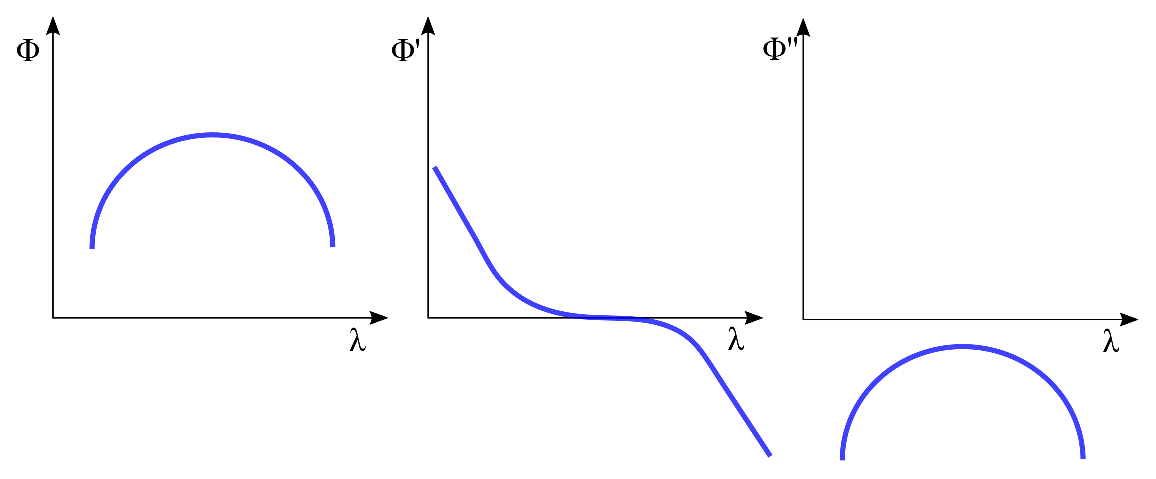
\includegraphics[width=\linewidth]{PhiConvex}
%    \caption[Connection one to one between $\lambda$ and $a$]{Representation of the convex functional $\Phi[\lambda]$ and its first and second derivative.}
%    \label{fig:PhiConvex}
%\end{figure}
%}


This argument is  valid for  any pair  of conjugate variables  and it
only depends on  the definition of the  conjugate variables introduced
in equation (\ref{relens1}).  It constitutes  the basic content of the DFT
when the relevant variable is the microscopic density operator.

Because the  connection is one  to one,  we may change  variables from
$\lambda$ to $a$.   However, the average $a$ is given  by a derivative
and such a  change of variables implies a loss  of information.  As we
know from the usual treatment in Thermodynamics \cite{Callen1960}, the
correct way to proceed is to  introduce the dimensionless entropy function $S[a]$ of
the given  level of description  as the (minus) Legendre  transform of
the thermodynamic potential in the form
\begin{align}
S[a] &=-\Phi[\lambda[a]]+\lambda[a] a
\label{entropya}\end{align}
The  relation of  this entropy  function $S[a]$  and the  Gibbs-Jaynes
entropy functional  ${\cal S}[\rho]$ in  (\ref{entropy}) is
simple. The  former is just  the later  evaluated at its  maximum, the
relevant ensemble (\ref{relens1}). This is
\begin{align}
S[a]={\cal  S}[\overline{\rho}]
\end{align}
Because  the  entropy   $S[a]$  is  the  Legendre   transform  of  the
thermodynamic  potential  $\Phi[\lambda]$,  we have  the  relationship
conjugate to (\ref{cg1})
\begin{align}
  \frac{\partial S}{\partial a}&=\lambda
\label{e3}
\end{align}


\section{The dynamics}\label{Sec:Grabert}

One important  objective within NESM
is the derivation of the governing dynamics of a set of
CG variables that describe the system at a mesoscopic or macroscopic
level of description  by starting from the microscopic  laws of motion
of the constituent atoms and  molecules of the system \cite{Kubo1991}.
In this quest, the projection  operator technique, as described in the
textbook by Grabert \cite{Grabert1982}, has  proved to be an extremely
useful  tool.   As  discussed   there,  there  are  essentially  three
different  types of  projection operator  theories, associated  to the
names  of   Mori  \cite{Mori1965},  Zwanzig   \cite{Zwanzig1961},  and
Kawasaki  and Gunton  \cite{Kawasaki1973},  with  increasing order  of
generality \cite{Grabert1982}. The Kawasaki-Gunton projection operator
allows one to  obtain nonlinear closed equations for  the averages of
the CG variables. The Zwanzig  projector is a special case
of  the Kawasaki-Gunton  projector  when the  selected variables  are,
instead of  the CG variables themselves,  the \textit{distribution} of
the  CG variables.  This results  into  a governing  equation for  the
probability distribution of CG  variables.  Finally, Mori projector is
obtained    from    Zwanzig     projector    in    near    equilibrium
situations\cite{Grabert1982,Kauzlaric2011a}.   The  resulting  dynamic
equations in  Mori theory are  linear and  allow one to  obtain simple
equations not only for the averages  of the CG variables, but also for
their correlation functions.

The projection operator technique  provides closed and exact equations
for the  evolution of the averages or probabilities  of the CG variables  with only one
assumption about  the initial  distribution of microstates,  which are
assumed   to  be   distributed   with  a   maximum  entropy   ensemble
\cite{Grabert1982}. The exact equations of  motion of the CG variables
contain a \textit{reversible  term} which is local in time  and an \textit{irreversible
integro-differential term} describing memory  about the past history of
the CG variables.  The memory  kernel is defined in microscopic terms,
and  it involves the so called \textit{projected
dynamics} which  is different, in  general, from the  usual Hamiltonian
dynamics of the system.

When the  selected CG  variables are  such that  they display  a clear
separation  of time  scales in  its dynamics  then it  is possible  to
resort  to the  Markovian  approximation, in  which  the memory  kernel
becomes proportional to  a Dirac $\delta$ function in time.   Such a separation
of  timescales  happens, in  general, when  the evolution  of the  CG
variables  is the  result of  many minuscule  and fast  contributions.
Under  the Markovian  approximation, the  resulting governing  dynamic
equations    are   nonlinear    differential   equations    for   the
nonequilibrium averages  of the  CG variables in  the Kawasaki-Gunton
projector or stochastic  differential equations (SDE) in  the Mori and
Zwanzig projectors.   Within the  Markovian approximation  one obtains
the  transport coefficients  governing  the irreversible  part of  the
dynamics in terms of the  time integral of correlation functions
  of the  time derivatives of  the CG variables.  These  formulas for
transport   coefficients  are   the  celebrated   Green-Kubo  formulas
\cite{Green1952,Kubo1957}.

\subsection{The Kawasaki-Gunton projection operator}
%In general it is possible to derive the evolution equation for a given
%dynamic  variable  by  using  the technique  of  projection  operators
%\cite{Kawasaki1973a,Grabert1982}. 
The projection operator method can be
understood, at its most fundamental level  as a way to approximate the
actual time dependent ensemble, which is the solution of the Liouville
equation, with a relevant  ensemble of the form (\ref{relens1}),
plus  a correction,  which  is the  responsible  for the  irreversible
behaviour. We  summarize   in  the   rest  of   this  section   the
time-dependent  projection  operator  technique as  presented  in  the
classical  textbook  by Grabert  \cite{Grabert1982}.   

The  aim is  to
derive equations of motion for  the time dependent average $a_i(t)$ of
the set of relevant variables $\hat{A}_i(z)$. The time dependent average
is
\begin{equation}
  a_i(t)={\rm Tr}[\rho_t\hat{A}_i],
  \label{ave}
\end{equation}
where $\rho_t$ is
the nonequilibrium solution of the Liouville equation. As it is shown
in  \cite{Grabert1982},  for  isolated systems  with a time-independent
Hamiltonian,  the   averages  (\ref{ave})  evolve  according   to  the
following closed exact equation

\begin{equation}
\frac{\partial }{\partial t} a_i(t)
= v_i(t) + \int_0^t dt' \sum_j K_{ij}(t,t') \lambda_j(t')
\label{ex}
\end{equation}
The reversible term is given by
\begin{equation}
v_i(t) = {\rm Tr}[\overline{\rho}_t  iL \hat{A}_i]
\label{vit}
\end{equation}
where $iL$ is the Liouville operator (\ref{iL}).

The  relevant
ensemble $\overline{\rho}_t$  is of  the form (\ref{relens1}),  with a
time   dependent  conjugate   variable  $\lambda(t)$.   The  conjugate
variables  $\lambda$ are  selected in  such  a way  that the  averages
$a(t)$ of the  real (i.e. the  solution of the Liouville equation) and of the relevant ensemble  coincide.  Note that
if   only  the   reversible  term   $v_i(t)$  would   be  present   in
equation (\ref{ex}), we would be  approximating the actual ensemble 
with a relevant  ensemble of
the form (\ref{relens1}), where the conjugate field $\lambda(t)$ is now
a function of time.  The error  in this approximation is, in fact, the
memory term which describes  irreversible behaviour.  The irreversible
term in equation (\ref{ex}) involves the memory kernel
\begin{equation}
K_{ij}(t,t') =
{\rm Tr}\left[\overline{\rho}_{t'} 
\left({\cal Q}_{t'} iL\hat{A}_j\right) G_{t't}
\left({\cal Q}_{t } iL\hat{A}_i\right)\right],
\label{ker}
\end{equation}
where   the  Kawasaki-Gunton   projection  operator   ${\cal  Q}_{t'}$
\cite{Kawasaki1973a,  Grabert1982}  applied  to an  arbitrary  function
$\hat{F}(z)$ is
\begin{align}
  {\cal Q}_{t'}\hat{F}(z) &= \hat{F}(z)- {\rm Tr}[\overline{\rho}_{t'} \hat{F}]
%\nonumber\\
-\sum_i(\hat{A}_i(z)-a_i(t'))\frac{\partial }{\partial a_i(t')}
{\rm Tr}[\overline{\rho}_{t'} \hat{F}]
\label{Q}
\end{align}
Finally, the time ordered projected propagator $G_{t't}$ is given by formal series
\begin{align}
  G_{t't}&=1
+\sum_{n=1}^\infty \int_{t'}^tdt_1\cdots\int_{t'}^{t_{n-1}}dt_n
 iL{\cal Q}_{t_n}\cdots  iL{\cal Q}_{t_1}
\nonumber\\
&\equiv T_+\exp\left\{\int_{t'}^t dt''  iL{\cal Q}_{t''}\right\},
\end{align}
where $T_+$ ensures that the operators are ordered from left to right as time increases.
equation   (\ref{ex}) is  a closed  exact equation  for the  time dependent
averages $a(t)$.  The only assumption  taken in deriving (\ref{ex}) is
that the initial  ensemble to be used in the  Liouville equation is of
the relevant form.  This is, it is assumed that  the only knowledge at
the initial  time is the value  of the average $a(0)$  and, therefore,
the  least   biased  initial   ensemble  is   of  the   relevant  form
(\ref{relens1}).  Therefore, the time  dependent average $a(t)$ of the
relevant variables $\hat{A}(z)$  is computed with the  solution of the
Liouville equation $\rho_t(z)$  with an initial condition  which is of
the relevant  form.  The relevant  ensemble is a functional  of $a(t)$
through  $\lambda(t)$.   The kernel  becomes  a  functional of  $a(t)$
through the relevant  ensemble.  

Although equation  (\ref{ex})  is a closed
equation, it is an integro-differential  equation which is difficult to
treat  in   general.   Nevertheless,  the  exact   transport  equation
(\ref{ex}) can  be approximated by  a memory-less equation  whenever a
clear separation  of timescales  exists between the evolution  of the
averages and  the decay of  the memory kernel. Under  this assumption
and the  neglect of terms of  order ${\cal O}( iL\hat{A}^3)$,  assumed to be
small due to  the slowness of the relevant variables,  one obtains the
Markovian equation \cite{Grabert1982}
\begin{equation}
  \frac{\partial}{\partial t}a_i(t) = v_i(t) + \sum_j D_{ij}(t) \lambda_j(t),
\label{ex2}
\end{equation}
where  the  dissipative matrix  is  given  by  the Green-Kubo  formula
\begin{equation}
D_{ij}(t)=\int_0^{\Delta t} dt'\left\langle 
{\cal Q}_t iL\hat{A}_j\exp\{iLt'\}{\cal Q}_t iL\hat{A}_i
\right\rangle^{\lambda(t)}
\label{dij}
\end{equation}
Here,  $\Delta t$ is  a  time large  compared  to the  decay  time of  the
correlation  integrand  but  short  in  front of  the  time  scale  of
evolution of  the relevant variables.  The  dissipative matrix depends
in general  on the  relevant variables  through the  relevant ensemble
and, as such, it is a function of time.  The dissipative matrix is, to
the  extent that  the  Markov property  holds,  positive definite  and
satisfies Onsager's reciprocity \cite{Grabert1982}. 

It is straightforward  to show that the  dynamic equations (\ref{ex2})
have  as  a  Lyapunov   function  the  entropy  (\ref{entropya})  and,
therefore,   the   dynamics   complies   with  the   Second   Law   of
Thermodynamics.  The  equations (\ref{ex2})  predict the decay  of any
initial value  of the  average of the  relevant variables  toward its
unique equilibrium  values. Forced situations may  be treated
with the present  formalism \cite{Grabert1982} but we  do not consider
them here for simplicity.

\subsection{Mori's Generalized Langevin equationation}
\label{Sec:Mori}
In the last section we introduced the Kawasaki-Gunton projection operator that allows one to obtain nonlinear closed equations of motion for the averages of a set of relevant variables. It is shown that the equations consist of two terms, a reversible term and irreversible one which contains the memory kernel. 
In this section we present a summary of Mori's theory \cite{Mori1965} which allows one to obtain not only linear dynamic equations for the averages of the relevant variables but also for their correlations. The Markovian approximation will be suppose as in the case of the nonlinear equations obtained with the Kawasaki-Gunton projection operator. 
%As we showed in Sec. \ref{Sec:Hamilton}, at a microscopic level of description we
%assume that  the system is  well described by CM and
%that the microscopic state $z=\{{\bf q}_i,{\bf p}_i,i=1,\cdots,N\}$ is
%given by the set of positions and  momenta of all the $N$ atoms in the
%system. The time evolution equation of the microstate is given by equation (\ref{zt}).
%\begin{align}
%  z_t = exp\{i{\cal L}t\}z_0
%\end{align}
%Hamilton's equations can be written in a very compact form as
%$  \dot{z}_t  =i{\cal  L}z_t$  where  $i{\cal  L}$  is  the  Liouville
%operator,  and $z_t$  is the  trajectory in  phase space  with initial
%condition $z_0$.  This  set of first order  differential equations has
%as a formal solution $ z_t = \exp\{i{\cal L}t\}z_0$.

Without  losing  generality,  we  will assume  that  the  equilibrium
average   of    the   CG    variables   vanish.    By    denoting  
$\hat{A}(t)=\hat{A}(z_t)$, the  evolution of these functions  in phase
space is given by
\begin{eqnarray}
\frac{d}{dt}{\hat{A}}(t)=\exp\{i{\cal L}t\}i{\cal L}\hat{A}(z_0)
\label{LA}
\end{eqnarray}

%At a macroscopic  level, we have  the system
%described with  a set  of $M$ CG variables  that are
%phase  functions  arranged  into  a column  vector  $\hat{A}(z)$  with
%components  $\hat{A}_\mu(z),\mu=1,\cdots,M$.   The  corresponding  row
%vector  is denoted  by $\hat{A}^T$,  where $T$  stands for  transpose.
%Without  loosing  generality,  we  will assume  that  the  equilibrium
%average   of    the   CG    variables   vanish.    By    denoting   by
%$\hat{A}(t)=\hat{A}(z_t)$, the  evolution of these functions  in phase
%space is given by
%\begin{eqnarray}
%\frac{d}{dt}{\hat{A}}(t)=\exp\{i{\cal L}t\}i{\cal L}\hat{A}(z_0)
%\label{LA}
%\end{eqnarray}

Mori's  exact  Generalized Langevin  equationation  (GLE)  is an  evolution
equation for the set of CG variables given by the following theorem\cite{Mori1965,Zwanzig2001,Kubo1991}
\begin{align}
\frac{d}{dt}\hat{A}(t) &= -L\esc C^{-1}(0)\esc \hat{A} (t)
%\nonumber\\
-\int_0^tdt'\Gamma(t-t')\esc  C^{-1}(0)\esc \hat{A} (t') +F^+(t),
\label{exact}
\end{align}
where the following matrices have been introduced
\begin{align}
L&=\langle \hat{A}i{\cal L}\hat{A}^T\rangle
\nonumber\\
C(0)&=\langle \hat{A}\hat{A}^T\rangle
\nonumber\\
\Gamma(t)&=\langle F^+(t)F^{+T}(0)\rangle,
\label{def}
\end{align}
where  $\langle\cdots \rangle$
denotes an equilibrium average
\begin{equation}
\langle\cdots\rangle\equiv \int dz\rho^{\rm eq}(z)\cdots,
\label{esc}
\end{equation}
$\rho^{eq}(z)$ is  the  equilibrium  ensemble, and $\hat{A}^T$ denotes the transpose of the column vector $\hat{A}$.
The so called projected force is given by
\begin{align}
F^+(t)&= \exp\{{\cal Q}i{\cal L}t\} {\cal Q}i{\cal L}\hat{A}  
\label{Proj}
\end{align}
The projection operator ${\cal Q}$ is defined as ${\cal Q}=1-{\cal P}$
where  ${\cal P}$  is Mori's  projector whose  effect on  an arbitrary
phase function $\hat{F}(z)$ is
\begin{align}
  {\cal P}\hat{F}(z) = \langle \hat{F}\rangle+ \langle \hat{F}\hat{A}^T \rangle\esc  C^{-1}(0)\esc  \hat{A}(z)
\label{PM}
\end{align}
The  Mori  projector  (\ref{PM})   satisfies  that  ${\cal  P}\hat{A}=
\hat{A}$ and  transforms an arbitrary  function of phase space  into a
linear combination  of the  CG variables.   The projected  forces have
zero  mean  and  are  uncorrelated  from
previous values of the CG variables, that is, 
\begin{align}
\langle  F^+  (t)\rangle&=0  
\nonumber\\
\langle \hat{A} F^+ (t)\rangle&=0 \quad\quad t\ge 0
\end{align}
%\section{Exact dynamic equation for correlations and averages}
The equilibrium time  correlation matrix of the CG variables is 
\begin{align}
  C(t)&=  \llangle \hat{A}(t)\hat{A}^T\rrangle
%=\llangle \left(\exp\{i{\cal L} t\}\hat{A}\right)\hat{A}^T\rrangle
\end{align}
If we  multiply the  exact equation (\ref{exact})  with $\hat{A}^T(z)$
and  average over  the equilibrium  ensemble, we  obtain a  closed and
exact equation for the correlation matrix of the CG variables
\begin{align}
  \frac{d}{dt}C(t)&=-L\esc C^{-1}(0)\esc C(t)
%\nonumber\\
-\int_0^tdt' \Gamma(t-t')\esc C^{-1}(0)\esc  C(t')
\label{exactC}
\end{align}

The GLE (\ref{exact}) allows  one to obtain
not only an equation for the correlation of the CG variables, but also
an equation for  their averages. If we multiply  (\ref{exact}) with an
initial ensemble $\rho_0(z)$ and integrate over the microstates $z$ we
obtain
\begin{align}
  \frac{d}{dt}a(t) &= -L\esc C^{-1}(0)\esc a(t)
%\nonumber\\
-\int_0^tdt' \Gamma(t-t')\esc  C^{-1}(0)\esc a(t')
\label{exactAve}
\end{align}
where the time-dependent average of the CG variables is defined as
\begin{align}
  a(t)&=\int dz \rho_0(z) \exp\{i{\cal L}t\}\hat{A}(z)
\end{align}
and we have assumed that the average of the projected force with respect
to the initial ensemble vanishes, i.e.
\begin{align}
\int dz\rho_0(z)\exp\{{\cal Q}i{\cal L}t\} {\cal Q}i{\cal L}\hat{A}(z)=0
\label{F0}
\end{align}
 Note that in deriving (\ref{exact})
one  assumes  that  the  dynamics   is  given  by  a  time-independent
Hamiltonian  with  a   well-defined  equilibrium  ensemble  $\rho_{\rm
  eq}(z)$.   Therefore,   both  (\ref{exactC})   and  (\ref{exactAve})
describe  the evolution  of  correlations and  averages toward  their
equilibrium values.

\subsubsection{The Markovian aproximation within Mori theory}
\label{Sec:Markov}
The   Markovian   approximation   assumes    that   there   exists   a
time-independent \textit{friction matrix} $M^*$ that
  contains the transport  coefficients of the CG  level of description
such that  the linear integro-differential term  in equation (\ref{exactC})
can  be  approximated  by  a  memory-less term,  also  linear  in  the
correlation matrix
\begin{align}
\int_0^tdt' \Gamma(t-t')\esc C^{-1}(0)\esc  C(t')&\simeq M^*\esc C^{-1}(0)\esc C(t)
\label{Markov1}
\end{align}
The  Markov approximation  (\ref{Markov1})  in  the GLE  (\ref{exact})
implies the following evolution equation for the CG variables
\begin{align}
  \frac{d}{dt}\hat{A}(t) = -\Lambda^*\esc \hat{A} (t) +F^+(t),
\label{SDE}
\end{align}
where the \textit{relaxation matrix} $\Lambda^*$ is defined as
\begin{align}
\Lambda^*\equiv(L+M^*)\esc C^{-1}(0)  
\label{Lambda}
\end{align}
The   approximation
(\ref{Markov1}) is equivalent to take
\begin{align}
  \Gamma(t) \approx M^*\delta^+(t)
\label{Markap}
\end{align}
where   the Dirac $\delta$ function
$\delta^+(t)$ is normalized as
\begin{align}
  \int_0^\infty dt \delta^+(t) =1
\end{align}
Under the  Markovian approximation,  equation  (\ref{Markap})  implies that
the projected  force is delta correlated  in time. As a  consequence, the
ordinary differential equation (\ref{SDE}) should be interpreted as a
stochastic  differential  equation (SDE)  for  times  larger than  the
correlation of $F^+(t)$.

By multiplying (\ref{SDE}) with an initial ensemble $\rho_0(z)$
satisfying (\ref{F0})
we obtain the following Markovian equation for the averages
\begin{align}
  \frac{d}{dt}a(t) = -\Lambda^*\esc a(t)
\label{AproxAve}
\end{align}
By  multiplying  (\ref{SDE})  with $\hat{A}(0)$  and  averaging  over
initial conditions sampled from  the equilibrium ensemble, one obtains
the evolution  equation of the  correlation matrix  under the
Markovian   approximation
\begin{align}
    \frac{d}{dt}C(t)&=-\Lambda^*\esc  C(t)
\label{AproxC}
\end{align}
The form of (\ref{AproxAve})  and (\ref{AproxC}) illustrates Onsager's
regression hypothesis, that states that (correlations of) fluctuations
decay  in  the  same  way  as  the  averages.   equation  (\ref{AproxAve}),
(\ref{AproxC}) show that the transport coefficients that appear in the
transport  equation for  the averages  are the  same as  the transport
coefficients  governing  the  correlations   of  the  fluctuations  in
equilibrium.


 The solution of (\ref{AproxC})  is given by
the exponential matrix 
\begin{align}
  C(t)=\exp\{-\Lambda^* t\}\esc C(0)
\label{Csol}
\end{align}
This is  the main  prediction of  Mori theory that  states that  for a
linear Markovian theory  the only possibility for a  correlation is to
decay  in an  exponential  matrix way.  This does  not  mean that  the
elements of  the correlation matrix  $C(t)$ decay as  $e^{-\alpha t}$,
because they are, in fact, the  sum of many exponential terms that may
lead even to quasi-algebraic decays of correlations, as in the case of
hydrodynamics.

We remark that  the Markovian equation  (\ref{AproxC}) cannot  hold at very
short  times,  because  at  $t=0$ the  exact  equation  (\ref{exactC})
implies
\begin{align}
    \frac{d}{dt}C(0)&=-L
\end{align}
which is only possible in  (\ref{AproxC}) if $M^*=0$. This paradoxical
result can  also be obtained  from equation  (\ref{Markov1}) because  if we
set $t=0$  in that  equation we obtain  again $M^*=0$.   Therefore, we
expect (\ref{AproxC}) to  hold only after a time  $t=\tau$ larger than
the decay  of the  memory kernel.   This is a  general feature  of the
Markovian  approximation showing  that correlations  will decay  in an
exponential, Markovian  way only  after the  time $\tau$  beyond which
memory is lost.  The value of  $\tau$ should be explicitly measured in
any procedure to validate the Markovian approximation.

The  usual  rationale  for   justifying  the  Markovian  approximation
(\ref{Markov1})  goes  as  follows  \cite{Grabert1982,Kubo1991}.   The
memory  kernel  $\Gamma(t-t')$ is  given  in  terms of  a  correlation
function  that it  is assumed  to decay  in a  typical molecular  time
scale.   On the  other hand,  it  is assumed  that the  timescale  of
evolution of the CG variables is  much larger than this molecular time
and, therefore,  within the  memory integral  $C(t')$ does  not change
appreciably and we may  approximate $C(t')\simeq C(t)$.  Therefore, we
have
\begin{align}
  \int_0^tdt' \Gamma(t-t')\esc c(t')&\simeq  \int_0^tdt' \Gamma(t-t')\esc  c(t)
\nonumber\\
&\equiv
M^+(t)\esc c(t)
\label{M+c}
\end{align}
where we have introduced the \textit{projected} Green-Kubo running integral
\begin{align}
M^+(t)&\equiv  \int_0^tdt' \Gamma(t') 
\nonumber\\
& =\int_0^tdt' \llangle \left(\exp\{{\cal Q}i{\cal   L}t'\}{\cal Q}i{\cal L}\hat{A} \right){\cal Q} i{\cal L}\hat{A}^T\rrangle 
\label{Mt}
\end{align}
and the normalized correlation matrix as
\begin{align}
  c(t)=C^{-1}(0)\esc C(t)
\label{cnorm}
\end{align}
that  at $t=0$  becomes  the identity  matrix.   The  Markovian
  assumption relies  on a  separation of time  scales. For  some model
  systems  (hydrodynamics of  unconfined  fluids \cite{Selwyn1971}  or
  Brownian  particles \cite{Mazur1970}),  one  can justify  rigorously
  such a  separation of  timescales as  some parameter  becomes small
  (wavelength or  ratio of masses) and  then usually the order  of the
  limits in the  parameter, time, and system size,  plays an important
  role.  In the  present dissertation,  we simply  assume that  the Markovian
  approximation is a sufficiently good one.


We will also consider
the \textit{unprojected} Green-Kubo running integral
\begin{align}
M(t)&\equiv  \int_0^{t} dt' \llangle \left(\exp\{i{\cal   L}t'\}i{\cal L}\hat{A} \right){\cal Q} i{\cal L}\hat{A}^T\rrangle
\label{Mtau}
\end{align}
where we distinguish $M(t)$ from  $M^+(t)$ because the former involves
the  unprojected  Hamiltonian  dynamics  $\exp\{i{\cal  L}t\}\hat{A}$,
while the later involves  the projected dynamics $\exp\{{\cal Q}i{\cal
  L}t\}\hat{A}$.  In  both $M^+(t)$  and $M(t)$  we recognize  a total
time derivative that allows to perform the time integral explicitly so
we have the alternative forms

\begin{align}
M^+(t)&=
  \llangle\left(\exp\{{\cal Q}i{\cal L}t\}  \hat{A}\right){\cal Q}i{\cal L}\hat{A}^{+T} \rrangle
\nonumber\\
M(t)&=
  \llangle\left(\exp\{i{\cal L}t\}  \hat{A}\right){\cal Q}i{\cal L}\hat{A}^{+T} \rrangle
\label{m+}
\end{align}
%where we  have used that  $ \langle \hat{A} (0)  F^{+T}(0) \rangle=0$.

Because the projected dynamics is in general more difficult to compute
than  the  unprojected  dynamics,  one  usually  resorts  to  a  large
separation  of  timescales  in  order  to approximate  the  projected
dynamics with  the unprojected  one \cite{Zwanzig1961,Selwyn1971,Mazur1970}.
For the  Markovian approximation  (\ref{Markov1}) to hold,  the matrix
$M^+(t)$ in  (\ref{M+c}) needs  to become the  time-independent matrix
$M^*$.  Note that  $M^+(t)$ vanishes at $t=0$ and after  a time $\tau$
should plateau to a constant value.  If one approximates $M^+(t)\simeq
M(t)$,  this   would  require  that   $M(t)$  would  have   a  plateau
itself.  However, this  is not  true because,  for an  ergodic system,
correlations computed with the unprojected dynamics decay to zero
\begin{align}
  \lim_{t\to\infty}M(t)&= \lim_{t\to\infty} \llangle\left(\exp\{i{\cal L}t\}  \hat{A}\right){\cal Q}i{\cal L}\hat{A}^{+T} \rrangle
\nonumber\\
&=
 \llangle  \hat{A}\rrangle\llangle{\cal Q}i{\cal L}\hat{A}^{+T} \rrangle=0
\end{align}
This  problem was  recognized already  by  Kirkwood as  the so  called
plateau problem \cite{Kirkwood1949,Espanol1993}  and limits the
use of the  unprojected Green-Kubo formula $M(t)$  for the calculation
of transport coefficients.

While $M(t)$  does not have  a plateau,  $M^+(t)$ may actually  have a
plateau  depending  essentially  on  the  spectrum  of  the  projected
evolution     operator    $\exp\{{\cal     Q}i{\cal    L}t\}$.      If
$|\hat{\psi}_\mu\rangle$  are  the   eigenvectors  of  corresponding
eigenvalues  $\lambda_\mu$  of  ${\cal   Q}i{\cal  L}$,  the  operator
$\exp\{{\cal Q}i{\cal L}t\}$ admits the eigendecomposition
\begin{align}
  \exp\{{\cal Q}i{\cal L}t\}&=\sum_\mu \exp\{-\lambda_\mu t\}|\hat{\psi}_\mu\rangle\langle\hat{\psi}_\mu|
\end{align}
in Dirac ket and bra notation, where the inner product is defined with
the equilibrium ensemble.  The matrix $M^+(t)$ then has the form
\begin{align}
  M^+(t)&=
\sum_\mu \exp\{-\lambda_\mu t\} \langle \hat{A}|\hat{\psi}_\mu\rangle
\langle\hat{\psi}_\mu|{\cal Q}i{\cal L}\hat{A}^{+T} \rangle
\end{align}
Note  that  the  equilibrium  eigenvector  $|\psi_0\rangle$  has  zero
eigenvalue.  For  the ergodic  unprojected dynamics  this is  the only
eigenvector of  null eigenvalue  but for  the projected  dynamics, the
zero  eigenvalue may  be  degenerate. In  other  words, the  projected
dynamics  may  have  other  conserved variables  in  addition  to  the
Hamiltonian that render the evolution  nonergodic with respect to the
equilibrium  measure.  Assume,  for  example, that  there  is only  one
eigenvector  $|\psi_1\rangle$  different   from  the  equilibrium  one
$|\psi_0\rangle$ of null eigenvalue. Then the infinite time limit is
\begin{align}
M^*&=\lim_{t\to\infty}  M^+(t)=\langle \hat{A}|\hat{\psi}_1\rangle
\langle\hat{\psi}_1|{\cal Q}i{\cal L}\hat{A}^{+T} \rangle
\end{align}
This is an expression for the transport coefficients $M^*$ in terms of
equilibrium averages.  Of  course, the calculation of  the spectrum of
${\cal Q}i{\cal L}$, or the identification of the additional conserved
quantities of  the projected dynamics is  not an easy task  in general
but it has been carried out for  a model system of a Brownian particle
in a  double well-potential \cite{Wu1989}. Also,  under a perturbation
scheme, the time integral of the correlation of the projected force of
a  Brownian particle  has  been carried  out  showing a  non-vanishing
plateau  \cite{Mazur1970}.    It  is   believed  that   the  projected
Green-Kubo matrix $M^+(t)$ has a well-defined plateau in general.

In  summary,  the projected  Green-Kubo  matrix  $M^+(t)$ may  have  a
well-defined plateau  but it is difficult  to evaluate it in  order to
get  transport  coefficients from  direct  MD  simulations, while  the
unprojected  Green-Kubo  matrix  $M(t)$  is easily  obtained  from  MD
simulations but  it usually  suffers from  the plateau  problem giving
ambiguous values for the transport coefficients.  In Chapter \ref{Chap:PBC} we will address the plateau problem in order to offer an alternative expression of transport coefficients in terms of corrected Green-Kubo formulas with no plateau problem by construction.

\section{Summary}
In this chapter we have introduced two important concepts that holds this dissertation. The first one, quasi-equilibrium, states that what we understand as equilibrium of a system depends on the time window we take. If the time of obervation is shorter than the time in which some variables evolve, we may use the variables as CG variables. 
Because the other variables evolve faster we may assume that are irrelevant for the selected level of description. 
Therefore, we say that the slow and faster variables evolve in different timescales, which is the second important concept of this chapter. 
Only when there is a well-separation of timescales we obtain tractable time evolution equation without memory terms. 
The approximation that allows one this simplification is known as the Markovian approximation. In this approximation the present does not depend on the past. 

This is known as Markovian descripcion to distinguish from the non-Markovian description in which the present state is determined by the past. 

Under the Markovian aproximation, we have obtained the general form of the memory-less dynamic equation of the CG variables using the Kawasaki-Gunton projection operator and the time-dependent equation for the correlation of the averages of the CG variables within Mori theory. 

%In the next chapter we will derive the dynamic equations for a set of CG variables of fluid in contact with a solid sphere. We will use the Kawasaki-Gunton formalism as well as in Chapter \ref{Chap:Planar}, where we will derive the discrete version of the hydrodynamic equations. \Note{Mencionar algo de Mori?} 

%We have introduced the relevant ensemble, $\bar{rho}$, based on the idea that the least biased probability distribution function is the one which maximazes the Shannon's entropy functional, which evaluated at its maximum (i.e. the relevant ensemble) is equal to the entropy function $S[a]$ obtained as the legendre transform of the thermodynamic potential $\Phi[\lambda]$.


%-----------------------------------------------------------------
%CHAPTER 2
%-----------------------------------------------------------------
\chapter{Nanoscale hydrodynamics theory for liquids near solids}\label{Chap:Theory}
\markboth{Nanoescale hydrodynamics theory for liquids near solids}{}
\epigraph{\textit{Le temps est une invention du mouvement. Celui qui ne bouge pas ne voit pas le temps passer.}}{Métaphysique des tubes \\ AMÉLIE NOTHOMB}


\section{Introduction}
As it was mentioned in the Introduction, Density Functional Theory (DFT) is a successful and well-established theory for the study of the structure of simple and complex fluids at equilibrium. The theory has been generalized to dynamical situations when the underlying dynamics is diffusive as in, for example, colloidal systems. However, there is no such a clear foundation for Dynamic DFT (DDFT) for the case of \textit{simple} fluids in contact with solid walls. 
In this chapter, we derive DDFT for simple fluids (fluids that obey  a Hamiltonian dynamics) by including not only the mass density field but also the momentum density field of the fluid. The standard projection operator method based on the Kawasaki-Gunton operator is used for deriving the equations for the average value of these fields. 

%The solid is described as featureless under the assumption that all the internal degrees of freedom of the solid relax much faster than those of the fluid (solid elasticity is irrelevant). 
%The fluid moves according to a set of {\em nonlocal} hydrodynamic equations that include explicitly the forces due to the solid. 
%These forces are of two types, reversible forces emerging from the free energy density functional, and accounting for impenetrability of the solid, and irreversible forces that involve the velocity of both the fluid and the solid. 
%These forces are localized in the vicinity of the solid surface. The resulting hydrodynamic equations should allow one to study dynamical regimes of simple fluids in contact with solid objects in isothermal situations.
We consider a fluid in contact with a 
large  spherical  solid  particle  in  order  to  address  fluid-solid
interactions.   In  usual DFT  approaches,  a  solid wall  is  usually
represented with  an {\em  external hard  potential}.  In  the present
description, a solid  wall is treated with  a coarse-grained procedure
in which  the atoms of the  wall are eliminated from  the description,
under the assumption that any elastic (or any other) degree of freedom
of the  solid is much faster  than the timescales  of the surrounding
fluid.  The  density functional that  emerges now depends not  only on
the density  field of the fluid  but also on the  overall CG variables
that we use to describe the solid.  For simplicity, we focus on a particularly simple particle shape, a solid spherical particle.  By considering the interaction of a  fluid with a solid sphere, we  may address the issue
of total momentum  conservation that may become rather  obscure if one
considers ``planar walls with infinite mass''. Of course, many of the
results that we obtain will be  easily transferred to planar walls, as
limits in which the  mass and the radius of the  solid sphere are both
very large.   In addition, we  take a spherical particle  because then
only the  position and  momentum of  the center of  mass of  the solid
particle is required in order  to have a coarse-grained description of
the solid.  For non-spherical particles,  it is necessary, in general,
to include also the orientation  and angular velocity of the particle,
as this is expected to play an important role in the dynamics.  Still,
even in the spherical particle case,  it may be important to introduce
angular velocity in order to  have accurate results.  However, for the
sake of simplicity and presentation  of the basic results, we restrict
ourselves in this chapter to the simplest case without angular variables
for the  solid particle. Also, and  for the sake of  simplicity, we do
not  consider the  intrinsic spin  of the  fluid, that  may become  an
important        relevant         variable        at        nanoscales
\cite{Hansen2009,Hansen2011a}.

The main result of this chapter is a set of dynamic equations that
govern the nonequilibrium \textit{averages} of hydrodynamic variables
and  the time-dependent  position  and momentum  of  the sphere.   The
dynamic equations  are of the form  of \textit{nonlocal} hydrodynamic
equations  for  the mass  and  momentum  density fields  coupled  with
Newton's  laws for  the center  of mass  of the  solid particle.   The
coarse-grained forces between the fluid  and the solid have reversible
and  dissipative contributions,  both localized  in a  boundary region
near  the  solid surface.   The  hydrodynamic  equations obtained  can
describe  the structuring  of the  fluid near  the solid  particle and
nonlocal flow effects that may be important at nano scales.

The  present  theory  is   both,  i)  a
generalization  of DFT  to dynamic  situations
\textit{in simple  fluids},
and ii) a full description,  at the coarse-grained hydrodynamic level,
of the solid-wall interactions.  The theory describes hydrodynamics at
scales  where the  molecular structure  of the  fluid is  apparent. At
these   scales   the   concept    of   boundary   condition   is   not
applicable. Instead, the interaction of  the fluid with the solid wall
is described with  reversible and irreversible forces  confined at the
vicinity of the wall.

Because  of the  two  aspects of  the present  theory  that have  been
already mentioned, i.e i) nonlocal hydrodynamics and ii) interactions
with solid walls, we discuss previous  work in these two areas in what
follows.

\subsection{Non-local hydrodynamics}
This   chapter    relies   on   the   pioneering    work   by   Piccirelli
\cite{Piccirelli1968}  who, following  Robertson \cite{Robertson1966},
derived  hydrodynamic   equations  explicitly  from   the  microscopic
dynamics  of  the fluid  system.   The  resulting   exact  hydrodynamic  equations
contained  nonlocal  transport  coefficients   defined  in  terms  of
Green-Kubo formulas.  In  similar terms, Grossmann \cite{Grossmann1970}
presented a derivation of nonlocal  hydrodynamics of simple fluids by
using  essentially  the  same  ideas behind  the  projection  operator
technique.    While   the    theory   provided   nonlocal   transport
coefficients, no connection was made in these early works with DFT,  which was not  yet developed in those  days.  Such
nonlocal  versions  for hydrodynamics  are  necessary  when the  flow
fields vary rapidly in space,  in the range of molecular correlations.
The  probing of  nanoscales in  MD simulations  has demonstrated  this
point                         very                        convincingly
\cite{Zhang2004,Hansen2007,Todd2008a,Hansen2011}.

\subsection{Fluid-solid  interactions}
Usually, at the hydrodynamic level  of description, the interaction of
a fluid with a solid is described through boundary conditions. Seminal
work  on  the understanding  of  boundary  conditions as  irreversible
interfacial processes  was given  by Bedeaux,  Albano, and  Mazur, who
introduced  interfacial  transport   coefficients  entering  into  the
boundary       conditions      \cite{Bedeaux1976}.        While      a
fluctuation-dissipation   theorem   was   formulated  for   the   slip
coefficient  \cite{Bedeaux1977},  which  could suggest  a  microscopic
evaluation  of  the  interfacial  boundary coefficients  in  terms  of
molecular dynamics, it  was not until the contribution  by Bocquet and
Barrat  that microscopic  expressions for  the interfacial  mechanical
\cite{Bocquet1994}  and   thermal  \cite{Barrat2003}   slip  transport
coefficients were given.   This work was a  conceptual breakthrough in
the extensive field of flow slip at solid surfaces.  However, a debate
was  initiated  by  Petravic  and  Harrowell  \cite{Petravic2007}  who
pointed out  that the  Green-Kubo expression  proposed by  Bocquet and
Barrat provides  not an intrinsic  solid-fluid property but  rather it
depends on the geometry of the setup. 
This is due, as it was mentioned in the Introduction to the fact that the
original expression reflects the total  fluid friction for shear flow,
including the slip friction at both  interfaces as well as the viscous
friction  in   the  fluid  \cite{Hansen2011,Kannam2011}. 
Hansen  et
al. \cite{Hansen2011} proposed to look at a thin slab of fluid near the
wall  and proposed  a phenomenological  Langevin equation  relating the
velocity of the  center of mass of  the fluid slab and  the force that
the wall exerts on the slab. The friction coefficient may be computed
from  equilibrium  MD  simulations  by  comparing  the  velocity-force
correlation to the velocity-velocity correlations of the slab. Another
recent approach has considered a generalized Langevin equation for the
velocity of a  single atom of the fluid near  a wall \cite{Huang2014}.
Recent  work  by   Ramos-Alvarado  et  al.   \cite{Ramos-Alvarado2016}
compares the above different approaches and concludes that simulations
are  very  sensitive  to  post-processing  issues,  leaving  the  story
somewhat inconclusive.

Our  theoretical approach  is not  restricted to  parallel flow  (i.e.
fluid   slabs)  as   is  typically   considered  in   simulation  work
\cite{Bocquet1994,Petravic2007,Hansen2011,Kannam2011,Ramos-Alvarado2016}.
Most derivations of  Green-Kubo expressions for friction  are based on
linear response theory where the  Hamiltonian is slightly perturbed by
an external  forcing \cite{Bocquet1994,Huang2014}.   We follow  here a
different  approach  in  obtaining   directly  the  full  hydrodynamic
equations from the  microscopic dynamics.  In this  way, the transport
coefficients  that  we obtain  are  the  ones  that really  enter  the
equations  of hydrodynamics  in  any general  flow configuration,  not
limited to homogeneous isotropic flat walls.

Note that  all the  mentioned work  on MD  simulations is  directed to
compute  the  transport  coefficients  that appear  in  slip  boundary
conditions.  When one descends to  the nanoscale, however, the picture
of the effect  of the solid-fluid interactions in terms  of a boundary
condition on an idealized surface  is questionable.  For the scales in
which nanostructure is  visible, e.g.  layering near the  wall, we aim
at  describing  the  fluid solid  interaction  through  coarse-grained
forces that extend  in a short range from the  solid. An early attempt
to use a ``friction field''  appeared in Ref. \cite{Sokhan2002}.
%In the second approach we consider that the friction force is transmitted throughout the nanotubes as a friction field Fz(r), i.e., the mean force on a particle at r in the direction of flow due to the wall. At equilibrium this force is zero.
Only when the  fluid is  macroscopic, we  would expect  these forces  to be
treated as  singular forces such that  its effect can be  described as
truly boundary  conditions on  the fluid. Recently, Camargo et al. \cite{CamargoBC2018} describe how the present theory gives rise to boundary conditions when the flows are macroscopic.

A precursor of the work presented in this chapter can be found in \cite{Cukier1980},  that considered a Brownian
hard  sphere in  a  sea of  small  hard spheres  and  used both,  Mori
projection  operator  and  kinetic   theory,  to  derive  hydrodynamic
equations  coupled to  the motion  of the  Brownian particle  (without
boundary conditions).   Our method is  more general in  that continuum
pair-wise   potentials   are   allowed   for,   and   the   nonlinear
Kawasaki-Gunton  projection operator  \cite{Kawasaki1973a} is  used for
the   coarse-graining   procedure   instead  of   the   simpler   Mori
projector \cite{Huang2014},   the   latter   being  limited   to   near
equilibrium linear  equations of motion \cite{Grabert1982}.   A theory
of  coarse-graining based  on  the Kawasaki-Gunton  projector gives  a
universal structure based on  the usual thermodynamic potentials.  The
use  of  the  Kawasaki-Gunton  projector  allows  us  to  express  the
reversible  part of  the dynamics  in a  way that  generalizes DFT to moving fluids.

Finally, Cadusch et al.  \cite{Cadusch2008}  show   that  the  use  of  a
nonlocal translation invariant kernel is not exempt  of problems in high
density fluids in strong nanoconfinement. They state: ``the fundamental
theoretical  challenge  that  remains   is  to  include  the  position
dependence  into   the  kernel   so  that   it  becomes   a  genuinely
inhomogeneous function  of space and  also to appropriately  model the
boundary conditions at the  fluid–wall interface, including stick/slip
boundary conditions.'' The present work addresses this challenge.


\section{The system and the relevant variables}
In this section we use the ToCG for describing hydrodynamically a liquid near a solid. 
Consider a liquid system of $N$ monoatomic molecules described
with the position and momenta of  their center of mass.  The molecules
are allowed to move through  space unrestrictedly. To avoid the issues
of  an infinite  number  of particles  required  in the  thermodynamic
limit, and to make closer contact with MD simulations,
we simply  assume that  the system  has periodic  boundary conditions.
Interacting with that sea of liquid molecules there is a group of $N'$
bonded atoms forming  what we would understand at a macroscopic level
as a solid object of spherical shape. 
At the microscopic level the system is described  by the set of all  positions  ${\bf  q}_i$  and  momenta  ${\bf  p}_i=m_i{\bf  v}_i$
($i=1,\cdots,N$) of the liquid atoms plus the positions ${\bf q}_{i'}$
and  momenta ${\bf  p}_{i'}=m_{i'}{\bf v}_{i'}$  ($i'=1,\cdots,N'$) of
the atoms  of the solid  sphere.  For  compactness we will  denote the
microstate in either  of the following forms $z$  or ${q,p,q',p'}$. From now, we
will distinguish  with a prime  the labels of  the atoms of  the solid
sphere from the  unprimed labels of the liquid  atoms.  The microstate
of  the  system  evolves  according to  Hamilton's  equations  with  a
Hamiltonian given by
\begin{eqnarray}
H(z) = \sum^N_i \frac{p_i^2}{2m_i} + \sum^{N'}_{i'} \frac{p_{i'}^2}{2m_{i'}}
+ U(z)
\label{H}
\end{eqnarray}
where the potential energy $U(z)$ is given by
\begin{align}
U(z)&=  V^{f}(q)+ V^{fs}(q,q')+ V^{s}(q')
\end{align}
We  assume   for  simplicity  a  pair-wise   potential  energy,  where
$V^{f}(q)=\frac{1}{2}\sum^{{NN}}_{i   j}\phi^{ll}_{ij}$   is   the
potential  of  interaction  between   liquid  atoms,  $  V^{ls}(q,q')=
\sum^{NN'}_{ii'}\phi^{ls}_{ii'}$  is  the   potential  of  interaction
between   liquid   atoms   and   solid   atoms,   and   $   V^{s}(q')=
\frac{1}{2}\sum^{{N'N'}}_{i' j'}\phi^{ss}_{i'j'}$ is the potential
of  interaction  between   the  atoms  of  the   solid  object.   Self
interaction of  the atoms  is not  considered, so  $\phi_{ii}=0$, etc.
There are  no external conservative  potentials acting on  the system,
although  they can  be  easily  introduced. We  do  not consider  such
external potentials  in order to  transparently discuss the  issues of
momentum conservation.

Note that at a microscopic level we do not have boundaries of
  any kind, we only have particles interacting with particles in free
(periodic) space.  In lab  situations, typically, liquids are contained
in flasks and other type of  solid objects that prevent the liquid from
leaking.  We could model a spherical  flask containing a liquid in very
much  the same  way  as we  are  going to  treat  the solid  spherical
particle  surrounded  by  the  (possibly  infinite  in  extension,  or
periodic)  liquid. A solid is
  regarded as a collection of  bounded atoms (that is, their relative
distances  do  not  increase  without   bound)  that  are  moving  and
vibrating. 
%The spherical  shape of the particle  should be understood,
%of course, in a statistical sense.

\subsection{The relevant variables}
We describe the system at a coarse grained level by selecting as
relevant variables the mass and momentum density fields  of the liquid
and  the   center  of  mass   position  and  momentum  of   the  solid
sphere. These are given by the following set of phase functions 
\begin{align}
  \hat{\rho}_{\bf r}(z) &=\sum^{N}_im\delta({\bf r}-{\bf q}_i)
&&\hat{\bf R}(z)=\frac{1}{N'}\sum_{i'}^{N'}{\bf q}_{i'}
\nonumber\\
  \hat{\bf g}_{\bf r}(z) &=\sum^{N}_i{\bf p}_i\delta({\bf r}-{\bf q}_i)
&&\hat{\bf P}(z)=\sum_{i'}^{N'}{\bf p}_{i'}
\label{CGvar}
\end{align}
where $\overline{\delta}({\bf r}-{\bf q}_i)$ is a coarse delta function as, for example, a normalized Gaussian.
In these phase  functions, the position ${\bf r}$ plays  the role of a
continuous index labeling  the phase function. The  position ${\bf r}$
may take any value in  $\mathbb{R}^3$, or its periodic counterpart, as
we  do  not  have  any  restriction to  the  possible  motion  of  the
particles. As was mentioned in \ref{Chap:NESM} the hamiltonian (\ref{H}) is also a relevant variable.

For the sake of simplicity, we do not include orientational degrees of
freedom of the  solid for the time being.  Note  that by selecting the
center of  mass variables of the  solid as the only  ones necessary to
describe the  state of the solid  we are implicitly assuming  that the
remaining  solid  degrees   of  freedom  are  much   faster  than  the
hydrodynamic  fields.   In  particular,  we assume  that  any  elastic
behaviour of the solid is  so rapidly decaying toward its equilibrium
state  that elastic  variables  do  not need  to  be  included in  the
description. Should this assumption be violated, the resulting dynamic
equations (not including  these elastic variables for the solid)
would probably  be non-Markovian.

A word is in order about a  model for the solid that is sometimes used
in  simulation work,  where the  solid  is  assumed to  be made  of
``frozen''  particles that  act  as simple  generators  of forces  not
reacting back  to the presence of  the liquid. In this  case, the solid
should be modeled as a static external field acting on the liquid. The
structure of the theory changes in this case as we will discuss later. 

\subsection{The time derivatives of the relevant variables}
The time derivatives  of the coarse variables play  a fundamental role
in the final structure of  the dynamic equations (\ref{ex2}). The time
derivative $  iL\hat{A}$ is  the result of  applying the  Liouville operator
(\ref{iL}) to the relevant variables.  In this section, we discuss the
particular  form of  $  iL\hat{A}$ for  the case  of  selected CG  variables
(\ref{CGvar}). The action of the Liouville operator on the CG variables gives \cite{Espanol2015a}
\begin{align}
    iL \hat{\rho}_{\bf r}(z) &= -\boldsymbol{\nabla}\esc\hat{\bf g}_{\bf r}(z)
\nonumber\\
iL  \hat{\bf g}_{\bf r}(z) &= -\boldsymbol{\nabla}{\cdot} \hat{{\bf K}}_{\bf r}(z)+
\hat{\bf F}^l_{\bf r}(z)
\label{ildens}
\end{align}
Here, the kinetic stress tensor is 
\begin{align}
  \hat{{\bf K}}_{\bf r}(z) &=\sum^{N}_i{\bf p}_i{\bf v}_i
\delta({\bf r}-{\bf q}_i)
\end{align}
and the total  force density $\hat{\bf F}^l_{\bf r}(z)$  on the liquid
is defined as
\begin{align}
  \hat{\bf F}^l_{\bf r}(z) &
=\sum_i^N-\frac{\partial U}{\partial {\bf q}_i}\delta({\bf r}-{\bf q}_i)
\label{Frtot}
\end{align}
We may decompose  this force density into the
force that  the liquid exerts on  the liquid plus the  force that the
solid   exerts  on  the   liquid,  this   is,  
\begin{align}
   \hat{\bf  F}^l_{\bf
  r}(z)&=\hat{\bf  F}^{\rm l\to  l}_{\bf r}(z)  +\hat{\bf  F}^{\rm s\to
  l}_{\bf r}(z) 
\nonumber\\
\hat{\bf F}^{\rm l\to l}_{\bf r}(z) &= \sum^{NN}_{ij}\hat{\bf F}_{ij}\delta({\bf r}-{\bf q}_i)
\nonumber\\
\hat{\bf F}^{\rm s\to l}_{\bf r}(z) &= \sum^{NN'}_{ij'}\hat{\bf F}_{ij'}\delta({\bf r}-{\bf q}_i)
\label{Fr}
\end{align}
where $\hat{\bf F}_{ij'}$ is the force  that atom $j'$ of the solid
exerts on  atom $i$ of  the liquid.   This is, $\hat{\bf  F}^{\rm l\to
  l}_{\bf r}(z)  $ is  the microscopic force  density that  the liquid
exerts on the liquid molecules that are around the point ${\bf r}$ and
$\hat{\bf F}^{\rm s\to l}_{\bf r}(z)$ is the microscopic force density
that the solid object exerts on the liquid at the point ${\bf r}$.

We may write the force that the liquid exerts on the liquid 
\begin{align}
  \hat{\bf F}^{\rm l\to l}_{\bf r}(z) &= \frac{1}{2}\sum^{NN}_{ij}\hat{\bf F}_{ij}
(\delta({\bf r}-{\bf q}_i)-\delta({\bf r}-{\bf q}_j))
\end{align}
where we  have used that  the indices are  dummy. By using  a standard
trick \cite{Schofield1982,Grabert1982}, we  may express the difference
of the Dirac $\delta$ functions in terms of a divergence
\begin{align}
\delta({\bf r}-{\bf q}_i)-\delta({\bf r}-{\bf q}_j)
    &=\int_0^1d\epsilon\frac{d}{d\epsilon}
\delta({\bf r}-{\bf q}_j-\epsilon{\bf q}_{ij})
\nonumber\\
    &=-\nabla\int_0^1d\epsilon{\bf q}_{ij}
\delta({\bf r}-{\bf q}_j-\epsilon{\bf q}_{ij})
\nonumber\\
\label{trick}
\end{align}

The liquid  force density  $\hat{\bf F}^{\rm  l\to l}_{\bf  r}(z)$ can
then be expressed  as the divergence of the  microscopic virial stress
tensor, that is,
\Note{Si equation (\ref{trick}), entonces el $\epsilon$ de equation (\ref{micfluxes}) tiene que ser negativo.}
\begin{align}
\hat{\bf F}^{\rm l\to l}_{\bf r}(z)&=-\boldsymbol{\nabla}{\cdot} \hat{\boldsymbol{\Pi}}_{\bf r}(z)
\nonumber\\
\hat{\boldsymbol{\Pi}}_{\bf r}(z)&\equiv \frac{1}{2}\sum^{N}_{ij}{\bf q}_{ij}\hat{\bf F}_{ij}
\int_0^{1}d\epsilon \delta({\bf r}-{\bf q}_i+\epsilon{\bf q}_{ij})
\label{micfluxes}
\end{align}
The time derivative of the momentum density (\ref{ildens}) becomes
\begin{align}
    iL\hat{\bf g}_{\bf r}(z)
    &=-\boldsymbol{\nabla}\cdot \hat{{\bf K}}_{\bf r}(z) - \boldsymbol{\nabla}\cdot \hat{{\bf     \Pi}}_{\bf r}(z) +  \hat{{\bf F}}^{\rm s\to l}_{\bf r}(z) \nonumber \\
    &= -\boldsymbol{\nabla}\cdot\left(\hat{{\bf K}}_{\bf r}(z)+\hat{{\bf \Pi}}_{\bf r}(z)\right) +\hat{{\bf F}}^{\rm s\to l}_{\bf r} \nonumber \\
    &=-\boldsymbol{\nabla}\cdot \hat{\boldsymbol{\sigma}}_{\bf r}+\hat{{\bf F}}^{\rm s\to l}_{\bf r},
\label{gls}
\end{align}
where     $\hat{\boldsymbol{\sigma}}_{\bf r}(z)=\hat{{\bf K}}_{\bf
r}(z)+\hat{\boldsymbol{\Pi}}_{\bf r}(z)$  is the microscopic stress
tensor of the fluid, that is,
\begin{align}
  \hat{\boldsymbol{\sigma}}_{\bf r}=
\sum^{N}_i{\bf p}_i{\bf v}_i
\delta({\bf r}-{\bf q}_i)
%\nonumber\\
+
\frac{1}{2}\sum^{N}_{ij}{\bf q}_{ij}\hat{\bf F}_{ij}
\int_0^{1}d\epsilon \delta({\bf r}-{\bf q}_i+\epsilon{\bf q}_{ij})
\label{sigma}
\end{align}
For the solid object we have that the action of the Liouville operator gives
\begin{align}
    iL\hat{\bf R}(z) &=\frac{\hat{\bf P}(z)}{M'}
  \nonumber\\
    iL\hat{\bf P}(z) &=-\int  d{\bf r} \hat{\bf F}^{\rm s\to l}_{\bf r}(z)
   \label{Pfsl}  
\end{align} 

Note  that the  total  momentum,  which is  defined  in  terms of  the
CG variables as
\begin{align}
  \hat{\bf P}_T&=\int d{\bf r} \hat{\bf g}_{\bf r}(z)+\hat{\bf P}(z),
\end{align}
satisfies $ iL\hat{\bf P}_T=0$ and is, therefore, a conserved quantity
of  the  microscopic   dynamics.   We  have  used   that  $\int  d{\bf
r}\boldsymbol{\nabla}\esc\hat{\boldsymbol{\sigma}}=0$ due to  Gauss theorem  and the  fact
that at the infinite we assume there are no fluid molecules. A similar
argument holds when the domain of integration is periodic.


Summarizing, the time derivatives of the relevant variables of the system are
\begin{align}
    iL \hat{\rho}_{\bf r}(z) &= -\boldsymbol{\nabla}\esc\hat{\bf g}_{\bf r}(z)
\nonumber\\
iL\hat{\bf g}_{\bf r}(z)
    &=-\boldsymbol{\nabla}\cdot \hat{\boldsymbol{\sigma}}_{\bf r}(z)+\hat{{\bf F}}^{\rm s\to l}_{\bf r}(z) \nonumber \\
    iL\hat{\bf R}(z) &=\frac{\hat{\bf P}(z)}{M}
  \nonumber\\
    iL\hat{\bf P}(z) &=-\int  d{\bf r} \hat{\bf F}^{\rm s\to l}_{\bf r}(z)
   \label{timeDerivatives}  
\end{align}

\section{The relevant ensemble and the grand potential}
In Sec. \ref{Sec:TheEntropy} we obtained that the ensemble which maximizes the Gibbs-Jaynes entropy function (\ref{entropy}) is of the type
\begin{equation}
\overline{\rho}(z) = \frac{1}{Z[\lambda]} \rho_0\exp\{-\lambda\!\cdot\!\hat{A}(z)\}
%\label{relens1}
\end{equation}
When the CG variables are those in (\ref{CGvar}), the relevant ensemble $\bar{\rho}(z)$ takes the form \Note{En el paper falta el $\rho_0$}
\begin{align}
  \overline{\rho}(z)&=\frac{1}{\Xi[\lambda]}\rho_0\exp\left\{-\beta H(z)\right\}
\nonumber\\
&\times
\exp\left\{-\beta\int d{\bf r}\left(\lambda_\rho({\bf r})\cdot\hat{\rho}_{\bf
    r}(z)+\boldsymbol{\lambda}_g{({\bf r})\cdot}\hat{\bf g}_{\bf r}(z)\right)\right\}
\nonumber\\
&\times
\exp\left\{-\beta \boldsymbol{\lambda}_{R}\esc\hat{\bf R}(z)
-\beta \boldsymbol{\lambda}_{P}\esc\hat{\bf P}(z)\right\}
\nonumber\\
\label{relensln}
\end{align}
The   normalization   factor   is  the   $\lambda$-dependent
grand-canonical partition function defined as
\begin{align}
  \Xi[\lambda]
  &\equiv
 \sum_{N=0}^\infty \frac{1}{N!h^{3N}}
\int dqdp dq'dp'
\nonumber\\
&\times\exp\left\{-\beta H-\beta \sum_{i=1}^Nm \lambda_\rho({\bf
    q}_i)-\beta \sum_{i=1}^N{\bf p}_i\esc\boldsymbol{\lambda}_g({\bf q}_i)\right\}
\nonumber\\
&\times\exp\left\{-\beta \boldsymbol{\lambda}_{R}\esc\hat{\bf R}(z)
-\beta \boldsymbol{\lambda}_{P}\esc\hat{\bf P}(z)\right\}
\label{xiln}
\end{align}
where we have introduced the coarse conjugate variables as
  \begin{align}
\lambda_\rho({\bf q}_i)&=
\int d{\bf r}\lambda_{\rho}({\bf r})\delta({\bf r}-{\bf q}_i)
\nonumber\\
\boldsymbol{\lambda_g}({\bf q}_i)&=
\int d{\bf r}\boldsymbol{\lambda}_g({\bf r})\delta({\bf r}-{\bf q}_i)
  \end{align}
The conjugate fields $\lambda$ of the CG variables (\ref{CGvar}) are fixed by the condition that the averages of the CG variables with the relevant ensemble coincide with the averages $\rho({\bf  r}),{\bf  g}({\bf
  r}),{\bf  R},{\bf  P}$  computed  with  the 
  solution of  the Liouville equation (we omit the time  dependence for simplicity). This conditions can be expressed as in equation (\ref{cg1}) through the followig expressions 
\begin{align}
  \rho({\bf r}) &=\frac{\delta \Phi [\lambda]}{\delta \lambda_\rho({\bf r}) }
&&{\bf R} =\frac{\partial \Phi [\lambda]}{\partial \boldsymbol{\lambda}_R }
\nonumber\\
  {\bf g}({\bf r}) &=\frac{\delta \Phi [\lambda]}{\delta \boldsymbol{\lambda}_g({\bf r}) }
&&{\bf P} =\frac{\partial \Phi [\lambda]}{\partial \boldsymbol{\lambda}_P }
\label{rgo}
\end{align}
where the $\lambda$-dependent {\em grand-canonical potential} is given, as in equation (\ref{PhiLambda}) by
\begin{eqnarray}
  \Phi [\lambda]\equiv-k_BT \ln\Xi [\lambda]
\label{oh}
\end{eqnarray}
As shown in Sec. \ref{Sec:TheEntropy}, there is a one to one connection between the CG variables and the conjugate ones becasuse the functional $\Phi[\lambda]$ is convex.  
Therefore, the  functionals $\lambda_{\rho}[\rho,{\bf  g},{\bf R},{\bf
  P}]$,   $\boldsymbol{\lambda}_g[\rho,{\bf   g},{\bf  R},{\bf   P}]$,
$\boldsymbol{\lambda}_R[\rho,{\bf      g},{\bf      R},{\bf      P}]$,
$\boldsymbol{\lambda}_P[\rho,{\bf g},{\bf  R},{\bf P}]$ exist  and are
unique.   We  can  therefore   switch  from  the  conjugate  variables
 to  the   relevant   variables  and  construct   the
 corresponding {\em hydrodynamic functional} given   by   the   Legendre    transform   of   the $\lambda$-dependent grand-canonical potential, that is,
\begin{align}
    {\cal H}[\rho,{\bf g},{\bf R},{\bf P}] =&
\Phi [\lambda_\rho,\boldsymbol{\lambda}_g,\boldsymbol{\lambda}_R,\boldsymbol{\lambda}_P]
\nonumber\\
    & -
\int d{\bf r}\rho({\bf r})\lambda_\rho({\bf r})
-
\int d{\bf r}{\bf g}({\bf r})\cdot\boldsymbol{\lambda}_g({\bf r})
\nonumber\\
    &    -\boldsymbol{\lambda}_R\cdot{\bf R}-\boldsymbol{\lambda}_P\cdot{\bf P}
\label{oleg}
\end{align}

Note that the hydrodynamic functional  is the negative of the corresponding entropy (\ref{entropya}) for the present level of description. Therefore, the equation (\ref{e3}) must be satisfied.

\begin{align}
  \lambda_\rho({\bf r}) &=-\frac{\delta {\cal H}}{\delta \rho({\bf r}) }
&&  \boldsymbol{\lambda}_R =-\frac{\partial {\cal H}}{\partial {\bf R} }
\nonumber\\
  \boldsymbol{\lambda}_g({\bf r}) &=-\frac{\delta {\cal H}}{\delta {\bf g}({\bf r}) }
&&  \boldsymbol{\lambda}_P =-\frac{\partial {\cal H}}{\partial{\bf P} }
\label{lno}
\end{align}

It is possible to find the explicit expression of $\lambda_{g}({\bf r})$ and $\boldsymbol{\lambda}_{\bf P}$ by performing the momentum integrals in equation (\ref{xiln}). Replacing in equation (\ref{xiln}) the Hamiltonian (\ref{H}) and the momentum of the solid (\ref{CGvar}) we obtain 
\begin{align}
\Xi[\lambda]
&\equiv
\sum_{N=0}^\infty \frac{1}{N!h^{3N}}
\int dqdpdq'dp'
\nonumber \\
&\times\exp\left\{-\beta U(z)-\beta \sum_{i=1}^Nm\lambda_\rho({\bf
    q}_i) -\beta \boldsymbol{\lambda}_{R}\esc\hat{\bf R}(z) \right\}
\nonumber \\
&\times
\exp\left\{-\beta \left(\sum_{i=1}^N\frac{{\bf p}_i^2}{2m_i} + \sum_{i=1}^{N'}\frac{{\bf p}_{i'}^2}{2m_{i'}} \right) - \beta \sum_{i=1}^N{\bf p}_i\esc\boldsymbol{\lambda}_g({\bf q}_i) 
-\beta \boldsymbol{\lambda}_P\sum_{i=1}^{N'}{\bf p}_{i'}\right\}
\end{align}
We may group the terms in this way
\begin{align}
\Xi[\lambda]
&\equiv
\sum_{N=0}^\infty \frac{1}{N!h^{3N}}
\int dqdpdq'dp'
\nonumber \\
&\times\exp\left\{-\beta U(z)-\beta \sum_{i=1}^Nm\lambda_\rho({\bf
    q}_i) -\beta \boldsymbol{\lambda}_{R}\esc\hat{\bf R}(z) \right\}
\nonumber \\
&\times
\exp\left\{-\beta \sum_{i=1}^N\left(\frac{{\bf p}_i^2}{2m_i} + {\bf p}_i\esc\boldsymbol{\lambda}_g({\bf q}_i)\right)\right\}
\exp\left\{-\beta \sum_{i=1}^{N'}\left(\frac{{\bf p}_{i'}^2}{2m_{i'}} + \boldsymbol{\lambda}_P{\bf p}_{i'}\right) \right\}
\end{align}
We perform the Gaussian integrals over momenta by using 
\begin{align}
\int_{-\infty}^{\infty} dx e^{-ax^2+bx}=\sqrt{\frac{\pi}{a}}e^{b^2/4a} 
\end{align}
reaching the following expression 
\begin{align}
\Xi [\lambda]
    \equiv&
 \sum_{N=0}^\infty \frac{1}{N!}
\int \frac{dq}{\Lambda^{3N}}\frac{dq'}{\Lambda^{3N'}}e^{-\beta U}
\nonumber\\
\times&\exp\left\{-\beta \sum_{i=1}^N\left(m\lambda_\rho({\bf
    r}_i)-\frac{m}{2}\boldsymbol{\lambda}_{g}^2({\bf q}_i)\right)\right\}
    \times\exp\left\{-\beta \left(\boldsymbol{\lambda}_R\cdot\hat{\bf R}-\frac{M'}{2}\boldsymbol{\lambda}_{P}^2\right)\right\},
\label{xiln2}
\end{align}
where we have introduced the thermal wavelength  
\begin{align}
\Lambda=\left(\frac{h^2\beta}{2\pi m}\right)^{\frac{1}{2}}
\label{ThermalWave}
\end{align}
Together with equation (\ref{rgo}) and equation (\ref{oh})
\begin{align}
  \rho({\bf r}) &=\frac{\delta \Phi [\lambda]}{\delta \lambda_\rho({\bf r}) } = \frac{1}{\Xi[\lambda]} \frac{\delta\Xi [\lambda]}{\delta \lambda_{\rho}({\bf r})} = m
  \nonumber\\
  {\bf g}({\bf r}) &=\frac{\delta \Phi [\lambda]}{\delta \boldsymbol{\lambda}_g({\bf r}) } =\frac{1}{\Xi[\lambda]} \frac{\delta\Xi [\lambda]}{\delta \boldsymbol{\lambda_g}({\bf r})} = -m\cdot\boldsymbol{\lambda}_g({\bf r})
 \nonumber\\
 {\bf P} &=\frac{\partial \Phi [\lambda]}{\partial \lambda_P} =\frac{1}{\Xi[\lambda]} \frac{\partial\Xi [\lambda]}{\partial \lambda_P} = -M'\cdot\lambda_P
\end{align}
This leads directly to the explicit form of the following conjugate variables
\begin{align}
 \boldsymbol{\lambda}_g({\bf r}) &= -\frac{{\bf g}({\bf r})}{\rho({\bf r})}=-{\bf v}({\bf r})
\nonumber\\
\boldsymbol{\lambda}_P &= -\frac{{\bf P}}{M'} = -{\bf V}
\label{nu}
\end{align}
and allows  one to interpret  these conjugate variables  as (negative)
velocities.  


We may express the gran potential (\ref{oh}) as a sum of two contributions
\begin{align}
\Phi [\lambda]&=  \Phi^{\rm pos}[\mu,\boldsymbol{\lambda}_R]
-\frac{M'}{2} {\boldsymbol{\lambda}_P}^2
\label{xpos1}
\end{align}
where we have defined the following grand potential
\begin{align}
\Phi^{\rm pos}[\mu,\boldsymbol{\lambda}_R]
&\equiv-k_BT\ln
 \sum_{N=0}^\infty \frac{1}{N!}
\int \frac{dq}{\Lambda^{3N}}\frac{dq'}{\Lambda^{3N'}}\nonumber\\
&\times
\exp\left\{-\beta  \left(U-\sum_{i=1}^N m\cdot\mu({\bf
    q}_i)+ \boldsymbol{\lambda}_R\cdot\hat{\bf R}\right)\right\}
\label{xpos}
\end{align}
and the chemical potential per unit mass has been introduced as
\begin{align}
  \mu({\bf r})&\equiv\frac{1}{2}\lambda_g^2({\bf r})-\lambda_\rho({\bf r})
\label{chempot}
\end{align}

Note that the gran potential (\ref{xpos}) is similar to the macrocanonical gran potential of a fluid, except for the presence of the solid degrees of freedom and the corresponding conjugate variable $\boldsymbol{\lambda}_R$. 

\section{The free energy}
The Legendre transform of the gran potential for a simple liquid gives the classic (free energy) density functional and we may pursue the same route in order to define the free energy density functional of a fluid in the presence of a solid sphere. The Legendre transform of the gran potential (\ref{xpos}) is
\begin{align}
  {\cal F}[\rho,{\bf R}]&\equiv  \Phi^{\rm pos}[\mu,\boldsymbol{\lambda}_R]
-\mu({\bf r})\frac{\delta\Phi^{\rm pos}}{\delta\mu({\bf r})}[\mu,\boldsymbol{\lambda}_R] 
-\boldsymbol{\lambda}_R\frac{\partial \Phi^{\rm pos}}{\partial \lambda_R}[\mu,\boldsymbol{\lambda}_R] 
\label{legPrev}
\end{align}
The derivatives we need of the functional (\ref{xpos}) are
\begin{align}
 \frac{\delta \Phi^{\rm pos}}{\delta \mu({\bf r})}[\mu,\boldsymbol{\lambda}_R]&=-
\langle \hat{\rho}_{\bf r}\rangle^{\mu,\boldsymbol{\lambda}_R}
\nonumber\\
  \frac{\partial \Phi^{\rm pos}}{\partial \boldsymbol{\lambda}_R}[\mu,\boldsymbol{\lambda}_R]&=
\langle \hat{\bf R}\rangle^{\mu,\boldsymbol{\lambda}_R}
\end{align}
where               the                averages               $\langle
\cdots\rangle^{\mu,\boldsymbol{\lambda}_R}$   are  defined   in  these
equations.  The second  derivatives of $ \Phi^{\rm pos}$  are given by
covariances  (see   equations  (\ref{cg1})-(\ref{covariances}))   and  this
implies that $\Phi^{\rm  pos}[\mu,\boldsymbol{\lambda}_R]$ is a convex
function.  Therefore, the  connection between $\langle \hat{\rho}_{\bf
  r}\rangle^{\mu,\boldsymbol{\lambda}_R},       \langle       \hat{\bf
  R}\rangle^{\mu,\boldsymbol{\lambda}_R}$         and        $\mu({\bf
  r}),\boldsymbol{\lambda}_R$ is  one to  one. Note also  that because
the phase functions  $ \hat{\rho}_{\bf r}, \hat{\bf R}$  do not depend
on particle's momenta, we have that the averages are given by
\begin{align}
  \langle \hat{\rho}_{\bf r}\rangle^{\mu,\boldsymbol{\lambda}_R} &={\rm Tr}[\overline{\rho}\hat{\rho}_{\bf r}]=\rho({\bf r})
\nonumber\\
  \langle \hat{\bf R}\rangle^{\mu,\boldsymbol{\lambda}_R} &={\rm Tr}[\overline{\rho}\hat{\bf R}]={\bf R}
\end{align}
Therefore,  we have  a one  to  one connection  between the  conjugate
variables  $\mu({\bf  r}),\boldsymbol{\lambda}_R$   and  the  averages
$\rho({\bf  r}),{\bf  R}$  of  the  CG  variables computed with the solution of the Liouville equation. 


Finally, we have the free energy functional ${\cal  F}[\rho,{\bf R}]$ of a structured fluid in the presence of a solid sphere as the following Legendre transform
\begin{align}
  {\cal F}[\rho,{\bf R}]&\equiv  \Phi^{\rm pos}[\mu,\boldsymbol{\lambda}_R]
+
\int d{\bf r}\rho({\bf r})\mu({\bf r})-\boldsymbol{\lambda}_R\cdot{\bf R}
\label{leg}
\end{align}
whose derivatives are given by 
\begin{align}
   \frac{\delta {\cal F}}{\delta\rho({\bf r})}[\rho,{\bf R}] &=\mu({\bf r})
\nonumber\\
   \frac{\partial {\cal F}}{\partial{\bf R}}[\rho,{\bf R}] &=-\boldsymbol{\lambda}_R
\label{Fd2}
\end{align}
We can obtain an expression for the  hydrodynamic functional (\ref{oleg}) replacing the terms $\Phi[\lambda]$, $\boldsymbol{\lambda}_g({\bf r})$, $\boldsymbol{\lambda}_P$, and $\lambda_R\cdot{\bf R}$ by the equations (\ref{nu}), (\ref{xpos1}), and using (\ref{leg}), respectively.
\Note{signo positivo antes del funcional de energía  libre}
\begin{align}
  {\cal H}[\rho,{\bf g},{\bf R},{\bf P}] =& 
  -\int d{\bf r} \rho({\bf r})\lambda_{\rho}({\bf r}) 
  +\int d{\bf r}\frac{{\bf g}^2({\bf r})}{\rho({\bf r})} 
  \nonumber\\
  &- {\cal F}[\rho,{\bf R}] -\int d{\bf r}\rho({\bf r})\mu({\bf r}) + \frac{{\bf P}^2}{2M'}
\end{align}
If we replace $\mu({\bf r})$ by the equation (\ref{chempot}) and use (\ref{nu}), we finally arrive to an expression of the hydrodynamic functional ${\cal H}$ which is the sum of a kinetic part and a ``potential'' part
\begin{align}
  {\cal H}[\rho,{\bf g},{\bf R},{\bf P}] &=   
  \underbrace{\int d{\bf r}\frac{{\bf g}^2({\bf r})}{2\rho({\bf r})} +\frac{{\bf P}^2}{2M'}}_{\rm kinetic}
  +\underbrace{{\cal F}[\rho,{\bf R}]}_{\rm potential}
\label{oleg2}
\end{align}
A we show in Appendix \ref{Ap:Forces}, $\boldsymbol{\lambda}_R$
is just the  average force on the solid due  to the fluid.  Therefore,
the ``potential''  part ${\cal  F}[\rho,{\bf R}]$ of  the hydrodynamic
functional  (\ref{oleg})  really  acts  as a  potential  energy  whose
negative gradient  gives the actual  force on the sphere.   For future
reference,  we  may also  compute  the  functional derivative  of  the
hydrodynamic functional ${\cal  H}$ with respect to  the density field
with the result
\Note{Creo que hay mal un signo $+\frac{v^2}{2}$}
\begin{align}
  \frac{\delta {\cal H}}{\delta\rho({\bf r})}[\rho,{\bf g},{\bf R},{\bf P}] &=    
-\frac{{\bf v}^2({\bf r})}{2}+  \frac{\delta {\cal F}}{\delta\rho({\bf r})}[\rho,{\bf R}]
\end{align}

The free energy functional is translationally invariant, that is,
\begin{align}
  {\cal F}[T_{\bf u}\rho,T_{\bf u}{\bf R}]&=  {\cal F}[\rho,{\bf R}]
\label{fa}
\end{align}
where the translation operator applied to any function is defined as
\begin{align}
  T_{\bf u}f({\bf r})&=f({\bf r}+{\bf u})
\end{align}
The  invariance  can be  shown  by  performing  a suitable  change  of
variables  inside the  phase space  integrals defining  the partition
function.  By taking the derivative with  respect to ${\bf u}$ in both
sides of equation  (\ref{fa}) and  setting afterwards ${\bf u}=0$ we obtain
the identity
\begin{align}
  \int d{\bf r}\frac{\delta {\cal F}}{\delta \rho_{\bf r}}
\boldsymbol{\nabla}\rho_{\bf r}&+\frac{\partial {\cal F}}{\partial {\bf R}}=0
\label{iden1}
\end{align}
This  identity will be  crucial in  order to  show that  total  momentum is
conserved by  the reversible part  of the dynamics.  

The calculation of the thermodynamic potential (\ref{xpos}) needed for
the evaluation of the free  energy functional ${\cal F}[\rho,{\bf R}]$
is very difficult  to perform in general and,  therefore, one needs to  model the
free energy functional based on intuition and previous experience. A
particularly simple model that takes into account the effect of the
fluid-solid interaction is given by
\begin{align}
  {\cal F}[\rho,{\bf R}]&={\cal F}_0[\rho]
+\int d{\bf r}\frac{1}{m}
\rho({\bf r})V({\bf r},{\bf R})
\label{modelnonlocalF}
\end{align}
where ${\cal F}_0[\rho]$ is the  free energy density functional of the
fluid in the absence of the solid, and all the fluid solid interaction
is  taken  into  account  through  the second  term  that  involves  a
\textit{coarse-grained   potential}   $V({\bf  r},{\bf   R})$.    This
potential  captures  the  effective (reversible)  interaction  between
solid and fluid atoms.  Note  that even for the case of
  an   ideal  gas   interacting  with   a  solid   sphere  the   model
  (\ref{modelnonlocalF})  does not  follow  straightforwardly from  the
  exact free energy (\ref{leg}) with (\ref{xpos}) due to the integrals
  over  the solid  degrees  of freedom  of  the interaction  potential
  between    ideal     gas    particles    and     solid    particles.
  equation (\ref{modelnonlocalF}) is just a natural  candidate to model the free
  energy $F[\rho,{\bf R}]$. The potential energy $V({\bf r},{\bf R})$
becomes infinite (or extremely large)  for the points ${\bf r}$ inside
the solid  sphere. Therefore, the last  term in (\ref{modelnonlocalF})
makes impossible the realization of density fields with nonzero value
inside the solid sphere (i.e.  leads to impenetrability of the solid).
The derivatives of the free energy model (\ref{modelnonlocalF}) are
\begin{align}
    \frac{\delta{\cal F}}{\delta\rho({\bf r})}=\mu_0({\bf r})+V({\bf r},{\bf R}),&&
%\nonumber\\
    \frac{\partial{\cal F}}{\partial{\bf R}}=-\int d{\bf r}\rho({\bf r}){\bf F}({\bf r},{\bf R})
\end{align}

\Note{¿No falta una m en el segundo término de la primera ecuación?}

where $\mu_0({\bf r})$ is the  usual chemical potential of the solvent
in the  absence of any  solid, and ${\bf  F}({\bf r},{\bf R})$  is the
effective force, deriving from the potential $V({\bf r},{\bf R})$ that
the solid sphere  with center of mass  at ${\bf R}$ exerts  on a fluid
atom at ${\bf r}$.



\section{The transport equations}
\label{Sec:Transequation}
In this section we obtain the transport equation for a fluid in contact with a solid sphere. In Sec. \ref{Sec:Grabert} we obtained an expression for the evolution of the selected variables using the technique of projection operators. This expression consists on two terms: the reversible part and the irreversible part. 

\subsection{Exact reversible dynamics}\label{Sec:ExactCont}
In this subsection we consider the reversible part for the case that the CG variables are those in equations (\ref{CGvar}).
For the mass density we have
\begin{align}
\left.\partial_t \rho({\bf r},t)\right|_{\rm rev}
&=  {\rm Tr}[\overline{\rho}_t  iL\hat{\rho}_{\bf r}] 
=-\boldsymbol{\nabla}\cdot {\bf  g}({\bf r},t)
\label{conrho}
\end{align}
where we have used equation (\ref{ildens}) and the fact that the relevant
ensemble average of $\hat{\bf g}_{\bf  r}$ is precisely  the momentum
density field ${\bf g}({\bf r},t)$.  On the other hand, and using again the equation (\ref{ildens}), the reversible
part of the momentum density evolution equation is
\begin{align}
\left.\partial_t {\bf g}({\bf r},t)\right|_{\rm rev}
&=  {\rm Tr}[\overline{\rho}_t  iL\hat{{\bf g}}_{\bf r}] 
\nonumber\\
&=-\boldsymbol{\nabla}\cdot  {\rm Tr}[\overline{\rho}_t \hat{{\bf K}}_{\bf r}] 
+  {\rm Tr}[\overline{\rho}_t  \hat{\bf F}^{\rm l}_{\bf r}]
\label{grev1}
\end{align}

We will compute the terms of equation (\ref{grev1}) taking advantage of the Galilean operator. 


The Galilean operator changes the velocity arguments from ${\bf v}_i\to {\bf v}_i+{\bf v}({\bf q}_i)$ for each $i$ fluid particle, that is,
\begin{align}
  {\cal G}\hat{F}({\bf q}_1,\cdots,{\bf q}_N;{\bf p}_1,\cdots,{\bf p}_N)
%\nonumber\\
=\hat{F}({\bf q}_1,\cdots,{\bf q}_N;{\bf p}_1+m_1{\bf v}({\bf q}_1),\cdots,{\bf p}_N+m_N{\bf v}({\bf q}_N))
\end{align}
The intuitive meaning of the Galilean operator is that when applied to a phase function gives how it is seen in a reference frame that moves with the flow field. Within any trace this is just a change of variables. Therefore, we have the property
\begin{align}
  {\rm Tr}[\bar{\rho}_t\hat{F}] &= {\rm Tr}[({\cal G}\bar{\rho}_t)({\cal G}\hat{F})] \nonumber \\
  \label{Gprop}
\end{align}
The action of the Galilean operator on the relevant variables is
\begin{align}
  {\cal G}\hat{\rho}_{\bf r} &= \hat{\rho}_{\bf r} \nonumber\\
  {\cal G}\hat{g}_{\bf r} &= \hat{g}_{\bf r} + {\bf v}({\bf r})\hat{\rho}_{\bf r} \nonumber \\
  {\cal G}\hat{\bf R}(z) &= \hat{\bf R}(z) \nonumber\\
  {\cal G}\hat{\bf P}(z) &= \hat{\bf P}(z)
\end{align}
Therefore, the action of ${\cal G}$ on the relevant ensemble is \Note{(En el paper aparece $\rho^{eq}$¿?)}
\begin{align}
  {\cal G}\overline{\rho}_t =
\frac{1}{\Xi[\lambda(t)]}\rho_0
\exp\left\{\beta\int d{\bf r}\mu({\bf r})\hat{\rho}_{\bf r}(z)\right\}
%\nonumber\\
\exp\left\{-\beta \boldsymbol{\lambda}_{R}(t)\esc\hat{\bf R}(z)
-\beta \boldsymbol{\lambda}_{P}(t)\esc\hat{\bf P}(z)\right\}
\label{resrelens}
\end{align}
where  the chemical  potential per  unit mass  has been  introduced in
equation  (\ref{chempot}). 
The  action  of the  Galilean  operator on  the
microscopic kinetic stress tensor is
\begin{align}
  {\cal G}\hat{{\bf K}}_{\bf r} &=
\hat{{\bf K}}_{\bf r} 
+{\bf v}({\bf r})\hat{\bf g}_{\bf r}
+\hat{\bf g}_{\bf r}{\bf v}({\bf r})
+{\bf v}({\bf r}){\bf v}({\bf r})\hat{\rho}_{\bf r}
\end{align}
Using (\ref{Gprop}) we have
\begin{align}
  {\rm Tr}[\bar{\rho}_t\hat{{\bf K}}_{\bf r}]={\rm Tr}[({\cal G}\bar{\rho}_t)({\cal G}\hat{{\bf K}}_{\bf r})]
\end{align}

By noting that the ensemble (\ref{resrelens}) is Gaussian in momenta, we have finally 
\begin{align}
  {\rm Tr}[\overline{\rho}_t \hat{{\bf K}}_{\bf r}] &=
{\bf v}({\bf r}){\bf v}({\bf r}){\rho}({\bf r})+\frac{k_BT}{m}\rho({\bf r})\boldsymbol{\delta}
\label{api}
\end{align}
where $\boldsymbol{\delta}$ is the unit  tensor.  The last term $ {\rm
  Tr}[\overline{\rho}_t \hat{\bf F}_{\bf r}]$  in equation (\ref{grev1}) is
computed  in   equation  (\ref{fllr})  of  the   Appendix \ref{Ap:Forces}.   By  collecting
(\ref{api})  and  (\ref{fllr})  into  the  momentum  density  equation
(\ref{grev1}) we obtain
\begin{align}
\left.\partial_t {\bf g}({\bf r},t)\right|_{\rm rev} 
&=-\boldsymbol{\nabla}\cdot\left({\bf v}({\bf r},t)  {\bf g}({\bf r},t)  \right)
-\rho({\bf r})\boldsymbol{\nabla}
\frac{\delta {\cal F}}{\delta\rho({\bf r})}[\rho,{\bf R}]
\label{grev}
\end{align}

Finally, the averages with the relevant ensemble of the solid object variables are
\begin{align}
{\rm Tr}[\overline{\rho}_t  iL\hat{\bf R}] 
&=\frac{\bf P}{M}
\nonumber\\
{\rm Tr}[\overline{\rho}_t  iL\hat{\bf P}] 
&=-\frac{\partial {\cal F}}{\partial {\bf R}}[\rho,{\bf R}]
\end{align}
where we have used equation (\ref{Fls}) in the Appendix \ref{Ap:Forces}.

By collecting the  above results, the reversible part  of the dynamics
has the form
\begin{align}
\left.  \partial_t\rho({\bf r})\right|_{\rm rev}&=-\boldsymbol{\nabla}\cdot{\bf g}({\bf r})
\nonumber\\
\left.  \partial_t{\bf g}({\bf r})\right|_{\rm rev}&=-\boldsymbol{\nabla}\cdot\left({\bf g}({\bf r}){\bf v}({\bf r})\right)
-\rho({\bf r})\boldsymbol{\nabla} \frac{\delta {\cal F}}{\delta\rho({\bf r})}[\rho,{\bf R}]
\nonumber\\
\partial_t\left. {\bf R}\right|_{\rm rev}&=\frac{\bf P}{M}
\nonumber\\
\partial_t\left.{\bf P}\right|_{\rm rev}&=-\frac{\partial {\cal F}}{\partial {\bf R}}[\rho,{\bf R}]
\label{rev}
\end{align}
These reversible  equations are exact  as no approximations  have been
made so far. We qualify these  equations as reversible because, as can
be  explicitly  shown,  they   conserve  the  hydrodynamic  functional
(\ref{oleg}), which  is minus the entropy corresponding
  to this level of description.



%Now, let us consider the average of the total force density on the liquid, equation (\ref{Frtot})
%\begin{align}
%{\bf F}^l_{\bf r} &\equiv{\rm Tr}[\overline{\rho}_t \hat{\bf F}^l_{\bf r}] =
% \langle \hat{\bf F}^l_{\bf r}\rangle^{\mu,\boldsymbol{\lambda}_R}
%\nonumber\\
%&=
%\frac{1}{\Xi[\mu,\boldsymbol{\lambda}_R]}
% \sum_{N=0}^\infty \frac{1}{N!}
%\int \frac{dq}{\Lambda^{3N}}\frac{dq'}{\Lambda^{3N'}}
%\left[\sum^{N}_{j}-\frac{\partial U}{\partial {\bf q}_{j}}\bar{\delta}({\bf r}-{\bf q}_j)\right]
%e^{-\beta U}
%\nonumber\\
%&\times \exp\left\{-\beta  \left( \boldsymbol{\lambda}_R\cdot\hat{\bf R}
%-\sum_{i=1}^N m\mu({\bf q}_i)\right)\right\}
%\end{align}
%where we have  used the definition of the average  with respect to the
%relevant ensemble,  after performing the momentum  integrals. Next, we
%realize that the  derivative of the Boltzmann factor  is the potential
%times the Boltzmann factor itself, this is
%\begin{align}
%{\bf F}^l_{\bf r}&=
%\frac{1}{\Xi[\mu,\boldsymbol{\lambda}_R]}
% \sum_{N=0}^\infty \frac{1}{N!}
%\int \frac{dq}{\Lambda^{3N}}\frac{dq'}{\Lambda^{3N'}}
%\exp\left\{-\beta  \left(\boldsymbol{\lambda}_R\cdot\hat{\bf R}
%-\sum_{i=1}^N m\mu({\bf   q}_i)\right)\right\}
%\nonumber\\
%&\times k_BT\sum^{N}_{j}\bar{\delta}({\bf r}-{\bf q}_j)\frac{\partial }{\partial {\bf q}_{j}}e^{-\beta U}
%\end{align}
%Integrate by parts to obtain
%\begin{align}
%{\bf F}^l_{\bf r}&=
%\frac{1}{\Xi[\mu,\boldsymbol{\lambda}_R]}
% \sum_{N=0}^\infty \frac{1}{N!}
%\int \frac{dq}{\Lambda^{3N}}\frac{dq'}{\Lambda^{3N'}}
%e^{-\beta U}
%\nonumber\\
%&\times
%k_BT\sum^{N}_{j}-\frac{\partial }{\partial {\bf q}_{j}}\left[\bar{\delta}({\bf r}-{\bf q}_j)
%\exp\left\{-\beta  \left( \boldsymbol{\lambda}_R\cdot\hat{\bf R}
%-\sum_{i=1}^N m\mu({\bf q}_i)\right)\right\}\right]
%\nonumber\\
%&=
%\frac{1}{\Xi[\mu,\boldsymbol{\lambda}_R]}
% \sum_{N=0}^\infty \frac{1}{N!}
%\int \frac{dq}{\Lambda^{3N}}\frac{dq'}{\Lambda^{3N'}}
%e^{-\beta U}
%\sum^{N}_{j}\exp\left\{-\beta  \left( \boldsymbol{\lambda}_R\cdot\hat{\bf R}
%-\sum_{i\neq j}^N m\mu({\bf   q}_j)\right)\right\}
%\nonumber\\
%&\times k_BT\left[-\frac{\partial }{\partial {\bf q}_{j}}\bar{\delta}({\bf r}-{\bf q}_j)
%\exp\left\{\beta   m\mu({\bf   q}_j)\right\}\right]
%\nonumber\\
%&=\frac{k_BT}{m}\boldsymbol{\nabla}\cdot \rho({\bf r})
%-\rho({\bf r})\boldsymbol{\nabla}\cdot\mu({\bf r})
%\label{fllr}
%\end{align}
%
%By  collecting (\ref{api})  and  (\ref{fllr})  into  the  momentum  density  equation (\ref{grev1}), and using (\ref{Fd2}), we obtain
%\begin{align}
%\left.\partial_t {\bf g}({\bf r},t)\right|_{\rm rev} 
%&=-\boldsymbol{\nabla}\cdot\left({\bf v}({\bf r},t)  {\bf g}({\bf r},t)  \right)
%-\rho({\bf r})\boldsymbol{\nabla}
%\frac{\delta {\cal F}}{\delta\rho({\bf r})}[\rho,{\bf R}]
%\label{grev}
%\end{align}
%
%In order to obtain the dynamics of the solid variables, we need to compute the average of the total force on the solid ${\bf F}^s$. We may follow identical steps as the case of the total force on the fluid ${\bf F}^f$ and obtain
%\begin{align}
%{\bf F}^s&={\rm Tr}[\overline{\rho}_t \hat{\bf F}^s]=
% \langle \hat{\bf F}^s\rangle^{\mu,\boldsymbol{\lambda}_R} 
%\nonumber\\
%&=\frac{1}{\Xi[\mu,\boldsymbol{\lambda}_R]}
% \sum_{N=0}^\infty \frac{1}{N!}
%\int \frac{dq}{\Lambda^{3N}}\frac{dq'}{\Lambda^{3N'}}
%\left[-\sum^{N'}_{i'}\frac{\partial U}{\partial {\bf q}_{i'}}\right]
%e^{-\beta U}
%\exp\left\{-\beta  \left(\sum_{i=1}^N m\mu({\bf
%    r}_i)+ \boldsymbol{\lambda}_R\cdot\hat{\bf R}\right)\right\}
%\nonumber\\
%&=
%\frac{1}{\Xi[\mu,\boldsymbol{\lambda}_R]}
% \sum_{N=0}^\infty \frac{1}{N!}
%\int \frac{dq}{\Lambda^{3N}}\frac{dq'}{\Lambda^{3N'}}
%\exp\left\{-\beta  \left(\sum_{i=1}^N m\mu({\bf
%    r}_i)+ \boldsymbol{\lambda}_R\cdot\hat{\bf R}\right)\right\}
%k_BT\left[\sum^{N'}_{i'}\frac{\partial }{\partial {\bf q}_{i'}}\right]e^{-\beta U}
%\nonumber\\
%&=
%\frac{1}{\Xi[\mu,\boldsymbol{\lambda}_R]}
% \sum_{N=0}^\infty \frac{1}{N!}
%\int \frac{dq}{\Lambda^{3N}}\frac{dq'}{\Lambda^{3N'}}
%e^{-\beta U}
%k_BT\left[-\sum^{N'}_{i'}\frac{\partial }{\partial {\bf q}_{i'}}\right]\exp\left\{-\beta  \left(\sum_{i=1}^N m\mu({\bf
%    r}_i)+ \boldsymbol{\lambda}_R\cdot\hat{\bf R}\right)\right\}
%\nonumber\\
%&=
%\frac{1}{\Xi[\mu,\boldsymbol{\lambda}_R]}
% \sum_{N=0}^\infty \frac{1}{N!}
%\int \frac{dq}{\Lambda^{3N}}\frac{dq'}{\Lambda^{3N'}}
%e^{-\beta U}
%\exp\left\{-\beta  \left(\sum_{i=1}^N m\mu({\bf
%    r}_i)+ \boldsymbol{\lambda}_R\cdot\hat{\bf R}\right)\right\}
%\left[\sum^{N'}_{i'}\frac{\partial }{\partial {\bf q}_{i'}}\right] \boldsymbol{\lambda}_R\cdot\hat{\bf R}
%\nonumber\\
%&=\boldsymbol{\lambda}_R
%\label{lf}\end{align}
%This  identity  allows  one  to  interpret  physically  the  Lagrange
%multiplier $\boldsymbol{\lambda}_R$ as the  force on the solid sphere.
%By  using (\ref{Fd2})  we obtain  that the  total force  on the  solid
%sphere is due to the gradient of the free energy functional
%\begin{align}
%{\bf F}^s&=-\frac{\partial  {\cal F}}{\partial{\bf R}}[\rho,{\bf R}]
%\label{Fls}
%\end{align}
%
%Therefore, the averages with the relevant ensemble of the solid object variables are
%\begin{align}
%{\rm Tr}[\overline{\rho}_t  iL\hat{\bf R}] 
%&=\frac{\bf P}{M}
%\nonumber\\
%{\rm Tr}[\overline{\rho}_t  iL\hat{\bf P}] 
%&=-\frac{\partial {\cal F}}{\partial {\bf R}}[\rho,{\bf R}]
%\end{align}
%where we have used the equation (\ref{Fls}).
%
%By collecting the  above results, the reversible part  of the dynamics
%has the form
%\begin{align}
%\left.  \partial_t\rho({\bf r})\right|_{\rm rev}&=-\boldsymbol{\nabla}\cdot{\bf g}({\bf r})
%\nonumber\\
%\left.  \partial_t{\bf g}({\bf r})\right|_{\rm rev}&=-\boldsymbol{\nabla}\cdot\left({\bf g}({\bf r}){\bf v}({\bf r})\right)
%-\rho({\bf r})\boldsymbol{\nabla} \frac{\delta {\cal F}}{\delta\rho({\bf r})}[\rho,{\bf R}]
%\nonumber\\
%\partial_t\left. {\bf R}\right|_{\rm rev}&=\frac{\bf P}{M}
%\nonumber\\
%\partial_t\left.{\bf P}\right|_{\rm rev}&=-\frac{\partial {\cal F}}{\partial {\bf R}}[\rho,{\bf R}]
%\label{rev}
%\end{align}
%These reversible  equations are exact  as no approximations  have been
%made so far. We qualify these  equations as reversible because, as can
%be  explicitly  shown,  they   conserve  the  hydrodynamic  functional
%(\ref{oleg}), which  is minus the entropy corresponding
%  to this level of description.

\subsection{Markovian irreversible dynamics}
While the  reversible part of  the dynamics (\ref{rev}) is  exact, the
irreversible  part  that we  consider  is  approximate
because  we assume a  Markovian dynamics.   Under the  Markovian
approximation in which the memory kernel is assumed to decay in a time
scale  short  as compared  to  the  time  scales of  the  hydrodynamic
variables,   the  irreversible   dynamics   is  given   by  the   term
$\sum_jD_{ij}\lambda_j$   in  equation   (\ref{ex2}).   Because   the  time
derivatives of  $\hat{\rho}({\bf r})$ and  $\hat{{\bf R}}$  are given in  terms of
momenta, which  are relevant variables  themselves, the effect  of the
projection operator in (\ref{Q}) is simply ${\cal Q} iL\hat{\rho}_{\bf r}=0$
and ${\cal Q}  iL\hat{{\bf R}}_{\mu}=0$ resulting in  a large simplification
of  the  friction  matrix.   The irreversible  part  of  the  dynamics
$\sum_jD_{ij}\lambda_j$ in equation (\ref{ex2}) now takes the form
\begin{align}
\partial_t  \left(
    \begin{array}{c}
\rho({\bf r})\\
\\
{\bf g}({\bf r})\\
\\
{\bf R}\\
\\
{\bf P}
    \end{array}
\right)_{\rm irr}
&=
-\left(\begin{array}{cccc}
  0&0 &0&0\\
\\
0 &\int d{\bf r}'M^{gg}_{{\bf r}{\bf r}'}&0&M^{gP}_{\bf r}\\
\\
  0&0 &0&0\\
\\
0&\int d{\bf r}' M^{Pg}_{{\bf r}'}&0&M^{PP}
\end{array}\right)
\left(    \begin{array}{c}
\frac{\delta {\cal H}}{\delta \rho_{{\bf r}'}}\\
\\
\frac{\delta {\cal H}}{\delta {\bf g}_{{\bf r}'}}\\
\\
\frac{\partial {\cal H}}{\delta {\bf R}}\\
\\
\frac{\partial {\cal H}}{\delta {\bf P}}
    \end{array}
\right)
\label{irr1}
\end{align}
where we have  used (\ref{lno}). The sum over  the continuum ``index''
${\bf  r}$ becomes  an integral.   The domain  of integration  of this
integral  is  $\mathbb{R}^3$,  including  the interior  of  the  solid
sphere. By  using the  results (\ref{lno}) and  (\ref{nu}) that  link the
functional derivatives of  the CG Hamiltonian with  respect to momenta
to the velocities, we obtain the following irreversible dynamics
\begin{align}
  \partial_t{\bf g}({\bf r})&=-\int d{\bf r}'M^{gg}_{{\bf r}{\bf r}'}
{\bf v}({\bf r}')-M^{gP}_{\bf r}{\bf V}
\nonumber\\
\frac{d}{dt}{\bf P}(t)&=-\int d{\bf r}' M^{Pg}_{{\bf r}'}{\bf v}({\bf r}')-M^{PP}{\bf V}
\label{IrrMark1}\end{align}
where the matrix elements are  defined in terms of Green-Kubo formulas
as
\begin{align}
  M^{gg}_{{\bf r}{\bf r}'}&=\frac{1}{k_BT}\int_0^{\Delta t} dt\langle 
{\cal Q}  iL\hat{\bf g}_{{\bf r}}(t){\cal Q}  iL\hat{\bf g}_{{\bf r}'}\rangle^\lambda
\nonumber\\
  M^{gP}_{{\bf r}}&=\frac{1}{k_BT}\int_0^{\Delta t} dt\langle 
{\cal Q}  iL\hat{\bf g}_{\bf r}(t){\cal Q}  iL\hat{\bf P}\rangle^\lambda
\nonumber\\
  M^{Pg}_{{\bf r}'}&=\frac{1}{k_BT}\int_0^{\Delta t} dt\langle 
{\cal Q}  iL\hat{\bf P}(t){\cal Q}  iL\hat{\bf g}_{{\bf r}'}\rangle^\lambda
\nonumber\\
  M^{PP}&=\frac{1}{k_BT}\int_0^{\Delta t} dt\langle 
{\cal Q}  iL\hat{\bf P}(t){\cal Q}  iL\hat{\bf P}\rangle^\lambda
\nonumber\\
\label{Ms}
\end{align}
Note that momentum conservation implies that the gain rate of the total momentum
of the fluid is equal to the loss rate of momentum of the particle
\begin{align}
  \int d{\bf r} iL\hat{\bf g}_{\bf r}&=-iL\hat{\bf P}
\label{iLgiLP}
\end{align}
The conservation of momenta then implies the following relationships between
elements of the dissipative matrix
\begin{align}
    M^{gP}_{{\bf r}}&=-\int d{\bf r}'M^{gg}_{{\bf r}{\bf r}'},&&
M^{PP}= - \int d{\bf r}M^{Pg}_{{\bf r}}
\end{align}
and this leads in equation (\ref{IrrMark1}) to 
\begin{align}
  \partial_t{\bf g}({\bf r})&=-\int d{\bf r}'M^{gg}_{{\bf r}{\bf r}'}\left({\bf v}({\bf r}')-{\bf V}\right)
\nonumber\\
\frac{d}{dt}{\bf P}(t)&=\int d{\bf r}\int d{\bf r}'M^{gg}_{{\bf r}{\bf r}'}\left({\bf v}({\bf r}')-{\bf V}\right)
%Esta última expresión se puede dejar en función de M^{Pg} y ver claramente que la derivada de P(t) será "igual" a la fuerza superficial {\cal S}
\label{IrrMark2}\end{align}
which contain only  the matrix element $M^{gg}_{{\bf  r}{\bf r}'}$ and are
manifestly  Galilean   invariant.   By  using  equations   (\ref{gls}),
(\ref{Pfsl}) {in} the  definition  of $M^{gg}_{{\bf  r}{\bf r}'}$  in
equation (\ref{Ms}),  and inserting  the result in  the equation  of motion
(\ref{IrrMark1}) one obtains
\begin{align}
\left.  \partial_t{\bf g}^\alpha({\bf r})\right|_{\rm irr}&= \boldsymbol{\nabla}_{\bf r}^{\beta}\boldsymbol{\Sigma}^{\alpha\beta}({\bf r}) +\boldsymbol{{\cal S}}^\alpha({\bf r}) 
\nonumber\\
\left.\frac{d}{dt}{\bf P}^\alpha(t)\right|_{\rm irr}&=-\int d{\bf r}'   \boldsymbol{{\cal S}}^\alpha({\bf r}')
\label{Irr}
\end{align}
where the fluid stress tensor is
\begin{align}
  \boldsymbol{\Sigma}^{\alpha\beta}({\bf r})&=
\int d{\bf r}'
\boldsymbol{\eta}^{\alpha\beta\alpha'\beta'}_{{\bf r}{\bf r}'}
\boldsymbol{\nabla}_{{\bf r}'}^{\beta'}{\bf v}^{\alpha'}({\bf r}')
\label{FluidStress}
\end{align}
and the \textit{irreversible surface force density} on the fluid is defined as
\begin{align}
  \boldsymbol{{\cal S}}^\alpha({\bf r})=&
-\int d{\bf r}'{\bf G}^{\alpha\alpha'\beta'}_{{\bf r}{\bf r}'}
\boldsymbol{\nabla}_{{\bf r}'}^{\beta'} {\bf v}^{\alpha'}({\bf r}')
\nonumber\\
&+\boldsymbol{\nabla}_{{\bf r}}^{\beta}\int d{\bf r}'{\bf H}^{\alpha\beta\alpha'}_{{\bf r}{\bf r}'}
( {\bf v}^{\alpha'}({\bf r}')-{\bf V}^{\alpha'})
%\nonumber\\
-\int d{\bf r}'
\boldsymbol{\gamma}^{\alpha\alpha'}_{{\bf r}{\bf r}'}( {\bf v}^{\alpha'}({\bf r}')
-{\bf V}^{\alpha'})
\label{Irreversibleforces}
\end{align}
Note that we use Einstein's sum over repeated indices convention.
In   these    expressions   we    have   introduced    the   following
\textit{nonlocal}  transport   coefficients:  the   viscosity  kernel
$\boldsymbol{\eta}_{{\bf r}{\bf r}'}$ (fourth  order tensor), the slip
kernels ${\bf  H}_{{\bf r}{\bf r}'},{\bf G}_{{\bf  r}{\bf r}'}$ (third
order  tensors), and  the  friction kernel  $\boldsymbol{\gamma}_{{\bf
    r}{\bf  r}'}$ (second  order  tensor).  They  are  defined by  the
Green-Kubo formulas
\begin{align}
  \boldsymbol{\eta}_{{\bf  r}{\bf r}'} &\equiv
\frac{1}{k_BT}\int_0^{\Delta t} dt'\langle 
{\cal Q}_t\hat{\boldsymbol{\sigma}}_{{\bf r}}(t')
{\cal Q}_t\hat{\boldsymbol{\sigma}}_{{\bf r}'}\rangle^{\lambda(t)}
\nonumber\\
{\bf H}_{{\bf r}{\bf r}'}&\equiv\frac{1}{k_BT}\int_0^{\Delta t} dt'
\langle {\cal Q}_t\hat{\boldsymbol{\sigma}}_{{\bf r}}(t')
{\cal Q}_t\hat{\bf F}^{\rm s\to l}_{{\bf r}'}\rangle^{\lambda(t)}
\nonumber\\
{\bf G}_{{\bf r}{\bf r}'}&\equiv\frac{1}{k_BT}\int_0^{\Delta t} dt'
\langle {\cal Q}_t\hat{\bf F}^{\rm s\to l}_{{\bf r}}(t')
{\cal Q}_t\hat{\boldsymbol{\sigma}}_{{\bf r}'}\rangle^{\lambda(t)}
\nonumber\\
\boldsymbol{\gamma}_{{\bf  r}{\bf r}'}&\equiv\frac{1}{k_BT}\int_0^{\Delta t} dt'
\langle 
{\cal Q}_t\hat{\bf F}^{\rm s\to l}_{{\bf r}}(t')
{\cal Q}_t\hat{\bf F}^{\rm s\to l}_{{\bf r}'}\rangle^{\lambda(t)}
\label{GK1}
\end{align}
These transport  kernels are state  dependent, i.e.  functions  of the
time  dependent  averages  of  the  relevant  variables,  through  the
dependence of  the relevant ensemble  on these averages.  The explicit
form of the projected currents appearing in these expressions is given
in the Appendix \ref{Ap:Projected}.

\section{The final equations of nanohydrodynamics} 
By collecting the reversible part  of the dynamics (\ref{rev}) and the
irreversible part  (\ref{Irr}) we  obtain the final  dynamic equations
for the relevant variables
\begin{align}
\partial_t\rho({\bf r})=&-\boldsymbol{\nabla}\cdot{\bf g}({\bf r})
\nonumber\\
\partial_t{\bf g}({\bf r})=&-\boldsymbol{\nabla}\esc{\left({\bf g}({\bf r}){\bf v}({\bf r})\right)}
-\rho({\bf r})\boldsymbol{\nabla}\frac{\delta {\cal F}}{\delta\rho({\bf r})}[\rho,{\bf R}]
+\boldsymbol{\nabla}\esc\boldsymbol{\Sigma}({\bf r})+\boldsymbol{{\cal S}}({\bf r})
\nonumber\\
\dot{\bf R}=&\frac{\bf P}{M}
\nonumber\\
\dot{\bf P}=&-\frac{\partial {\cal F}}{\partial {\bf R}}
-\int d {{\bf r}}\boldsymbol{{\cal S}}({\bf r})
\label{finaleq}
\end{align}
where  the   free  energy  functional  ${\cal   F}[\rho,{\bf  R}]$  is
introduced  in  equation (\ref{leg}),  the  velocity  field is  ${\bf  v}({\bf
  r})={\bf  g}({\bf  r})/\rho({\bf  r})$,   the  fluid  stress  tensor
$\boldsymbol{\Sigma}({\bf  r})$ is  given in  (\ref{FluidStress}), and
the irreversible  force $\boldsymbol{{\cal  S}}({\bf r})$ is  given in
equation (\ref{Irreversibleforces}).

Equations   (\ref{finaleq}), (\ref{GK1}),   (\ref{Irreversibleforces}) 
are the  main results of the present  chapter.  They describe
the isothermal nonlocal  hydrodynamics of a  simple fluid coupled with
the motion of an immersed structureless solid sphere.  These equations
generalize equationilibrium DFT for a simple fluid to
nonequilibrium situations in  which the fluid may be  moving around a
solid  sphere.  The  only approximation  that  has been  taken in  the
derivation is the Markovian approximation that neglects memory effects
in the dissipative part of the dynamics.

Let  us  discuss  the  physical  meaning of  the  different  terms  in
equations  (\ref{finaleq}).  The  equation for  the evolution  of the  mass
density field is  just the continuity equation.  The  equation for the
momentum density field involves the  usual convective term plus a term
involving  the  gradient of  the  functional  derivative of  the  free
energy.  This term describes both,  the ``pressure gradient'' term and
the reversible coupling between the  fluid and solid sphere. The usual
pressure gradient term of the Navier-Stokes equations is obtained when
one  uses   a  local   free  energy  functional   as  will   be  shown
elsewhere.               The                viscous               term
$\boldsymbol{\nabla}\esc\boldsymbol{\Sigma}$  
describes   the  internal   friction   of  the   fluid   due  to   its
self-interaction.  This  viscous term involving second  derivatives is
the usual viscosity term of the Navier-Stokes equations, which is here
expressed in a  nonlocal form.  The use of  nonlocal viscosities has
been   advocated  recently   in   the   field  of   nano-hydrodynamics
\cite{Zhang2004,Hansen2007,Todd2008a,Hansen2011}.  A phenomenological
alternative to address flow problems where density is inhomogeneous is
to keep using  local hydrodynamics with the viscosity of  the bulk but
evaluated at the local values of the density\cite{Bitsanis1987}. While
this   may    lead   to    reasonable   results   (but    not   always
\cite{Bitsanis1990}), the present  microscopically derived model seems
to have a firmer basis. The  fourth order viscosity tensor is given in
terms  of the  correlation of  the  fluctuations of  the fluid  stress
tensor.  Away from the walls, it is expected that the viscosity tensor
becomes fully isotropic and dependent only on the distance between the
points ${\bf r},{\bf r}'$.

The  force  density  $\boldsymbol{{\cal S}}({\bf  r})$  involving  the
nonlocal transport  kernels ${\bf H}_{{\bf r}{\bf  r}'}$, ${\bf G}_{{\bf r}{\bf r}'}$, 
$\boldsymbol{\gamma}_{{\bf  r}{\bf r}'}$ describes the
irreversible interaction between  the solid and the  fluid.  Note that
these  kernels are  defined  in (\ref{GK1})  in  terms of  correlations
involving the  force density $\hat{\bf  F}^{s\to l}_{\bf r}$  that the
solid sphere  exerts on the  liquid molecules.  These terms  should be
understood,  therefore,  as  the   responsible  for  transmitting  the
irreversible  forces that  the solid  sphere exerts  on the  fluid. The
force density $\hat{\bf F}^{\rm s\to  l}_{\bf r}(z)$ will be different
from zero only for  those points ${\bf r}$ that are  near of the solid
sphere.  This means  that the transport kernels  ${\bf G}_{{\bf r}{\bf
    r}'},{\bf  H}_{{\bf  r}{\bf r}'},\boldsymbol{\gamma}_{{\bf  r}{\bf
    r}'}$  are highly  localized  near  the atoms  of  the solid  that
interact with the  fluid.  Note that  \textit{the concept of
  surface of the solid does not  enter this theory}.  There is no such
a well-defined  surface in  microscopic terms.  However,  this surface
can  be defined  \textit{operationally}  by looking  precisely at  the
singular behaviour of the above  transport kernels.  Indeed, the force
density $\hat{\bf  F}^{\rm s\to l}_{\bf  r}(z)$ will be  a fluctuating
vector on the surface of the solid sphere.  If the interaction between
fluid and solid atoms is purely  repulsive, this force will be most of
the time  directed outwards the surface  of the solid sphere.   At the
same time,  because the interaction  between solid and fluid  atoms is
singular  as  their  separation  vanishes, we  expect  that  $\hat{\bf
  F}_{\bf r}^{\rm  s\to l}$ will  diverge as ${\bf r}$  approaches the
solid boundary.  This  divergence will be reflected  in divergences of
the  transport kernels  as  ${\bf  r}$ or  ${\bf  r}  '$ approach  the
boundary  of  the  solid.   In   a  similar  way,  the  stress  tensor
$\hat{\boldsymbol{\sigma}}_{\bf r}$  that depends  only on  fluid atom
coordinates will be nonzero only outside the solid sphere because the
interaction with  the solid sphere  refrains to have  liquid molecules
inside the solid sphere (more  on this later).  Therefore, the surface
of the solid may be characterized  by the singularity of the transport
coefficients   ${\bf  H}_{{\bf   r}{\bf   r}'},{\bf  G}_{{\bf   r}{\bf
    r}'},\boldsymbol{\gamma}_{{\bf r}{\bf  r}'}$ and the  vanishing of
$\boldsymbol{\eta}_{{\bf r}{\bf r}'}$.

The force density and the stress tensor are assumed to vary in time in
a time  scale much shorter  than the typical  timescale in  which the
mass  and  momentum density  of  the  solvent,  and the  position  and
momentum  of  the solid  sphere  particle  appreciably changes.   This
separation of timescales is at the  core of the Markovian form of the
evolution   of   the   CG   dynamics  in   the   projection   operator
technique. Whether the selected  relevant variables do actually comply
with  this separation  of time  scales can  only be  assessed from  the
validity of the  predictions of the resulting theory  as compared with
actual   simulations  or   experiments.   Note,   however,  that   for
slowly varying flow  configurations, as  those attained  in steady
states, the Markovian approximation should be reasonably fulfilled.

\subsection{Conserved quantities, $H$-theorem and the equilibrium state}
The equations  (\ref{finaleq}) are the equations  of hydrodynamics in
the  presence of  a solid  spherical particle.  We
stress  that  the  above  equations conserve  total  mass  and
momentum, given by
\begin{align}
  M_T&=M'+\int d{\bf r}\rho({\bf r})
\nonumber\\
{\bf P}_T&={\bf P}+\int d{\bf r}{\bf g}({\bf r})
\end{align}
Mass conservation  follows immediately  from the  continuity equation.
Momentum  conservation  is  a  consequence  of  the  invariance  under
translations   of   the   free    energy   functional   expressed   in
equation  (\ref{iden1})  that  ensures  that the  reversible  part  of  the
dynamics  conserves momentum.   The irreversible  part conserves  also
total  momentum because  the
momentum lost by the fluid is gained by the solid sphere.

In  addition, the  function ${\cal H}$  evolves in time  in a
strictly decreasing way, that is,
\begin{align}
  \frac{d{\cal H}}{dt}(t)\le 0,
\label{Htheo}\end{align}
where  the  equality sign  occurs  when  the  system has  reached  its
equilibrium state.  This  is because, while the reversible  part of the
dynamics conserves  ${\cal H}$,  the irreversible part  of the
dynamics  fulfills  (\ref{Htheo}), due  to  the positive  semidefinite
character of  the friction matrix.  

As a consequence, the equilibrium state of equations (\ref{finaleq}) is the
one that minimizes ${\cal H}$ subject to the constraints of giving the
actual values of the total mass  and momentum.  In order to obtain the
equilibrium values of  the relevant variables, one  should minimize the
following functional without constraints
\begin{align}
  {\cal H}-\mu_0\int d{\bf r} \rho({\bf r})-{\bf V}_0\cdot\left[\int d{\bf r}{\bf g}({\bf r})+{\bf P}\right]
\end{align}
where    $\mu_0,{\bf   V}_0$    are    the   corresponding    Lagrange
multipliers. Setting  to zero the derivatives of  the above functional
gives  \Note{En la primera expresión que es la derivada con respecto a $\rho(r)$ no le falta un término $-V_0{\int d{\bf r}\bf v(r)}$? Luego se irá haciendo $V_0=0$}
\begin{align}
  \frac{{\bf v}^2({\bf r})}{2}
+\frac{\delta {\cal F}}{\delta\rho({\bf r})}[\rho,{\bf R}]-\mu_0&=0,\quad
&&\frac{\partial {\cal F}}{\partial {\bf R}}[\rho,{\bf R}]=0
\nonumber\\
{\bf v}({\bf r})-{\bf V}_0&=0,\quad
&&{\bf V}-{\bf V}_0=0
\label{eq01}
\end{align}
This means that the state of equilibrium has a constant velocity field
equal  to the  velocity  of  the solid  particle  and, without  losing
generality, we may take ${\bf V}_0=0$.  We then have the following two
coupled  equations for  the equilibrium  value that  take the  density
field and the position of the sphere
\begin{align}
\frac{\delta {\cal F}}{\delta\rho({\bf r})}[\rho,{\bf R}]&=\mu_0,\quad
&&
\frac{\partial {\cal F}}{\partial {\bf R}}[\rho,{\bf R}]=0
\label{eq1}
\end{align}
From equations   (\ref{Fd2}), the first equation  (\ref{eq1}) simply states
that  the equilibrium  state  has  a constant  value  of the  chemical
potential $\mu({\bf  r})=\mu_0$ while the second  equation states that
the total force on the solid  sphere vanishes at equilibrium. This set
of two  coupled equations should be  understood as a set  of nonlinear
equations for  the equilibrium density  field $\rho({\bf r})$  and the
equilibrium value of the center  of mass position ${\bf R}$ of the sphere.  Translational
invariance of the system implies that  if ${\bf R},\rho({\bf r})$ is a
solution of (\ref{eq1}), then  ${\bf R}+{\bf u},\rho({\bf r}+{\bf u})$
is also  a solution.   Therefore, without loose  of generality  we may
choose the origin of coordinates at the center of the sphere and ${\bf
  R}=0$. Then  the equilibrium  density field is  the solution  of the
first equation.   Note that  for realistic models  of the  free energy
functional,  the  density field  will  display  oscillations at  short
length scales due  to the packing of the fluid  near the solid sphere.


In the  present theory,  the equilibrium  profile is  the one  that is
reached  at  long times  due  to  the  evolution of  the  hydrodynamic
equations.  In this subsection, we have shown how the theory presented
contains  the usual  prescription  to obtain  the equilibrium  density
profile in  DFT by minimizing the  free energy
functional.

\subsection{Approximating the relevant ensemble averages and projected
  currents}
It  should be  remarked that  the theory  presented is  valid, as  the
H-theorem  clearly testifies,  for the  decaying dynamics  toward the
equilibrium state in isolated systems. It is, therefore, a theory that
describes, given initial nonequilibrium values for  the averages of the CG variables,
the subsequent  average evolution toward equilibrium.   One situation
in which  we will  be interested  is when the  solid particle  is very
large and  massive.  In these situations, we may assume
that the spherical particle has initial (average) position ${\bf R}_0$
and initial  (average) momentum  ${\bf P}_0=0$ and  that, for  all the
decay evolution of the hydrodynamic fields, these values do not change
appreciably because the  forces that the fluid exerts  on the particle
during  its evolution  are  not sufficiently  strong  to modify  these
variables substantially.

In principle, the  relevant ensemble depends (in a  functional way) on
the averages of all the relevant  variables of the system.  As this is
unduly complicated, we  take the approximation in  which the transport
kernels are evaluated for the {\em equilibrium} values of the relevant
variables. In  this doing, we assume  that for any other  value of the
average value of the relevant variables  obtained in the course of the
dynamics,  the  transport  kernels  do not  change  appreciably.   The
equilibrium  values  of  the  average  relevant  variables  have  been
obtained in  equation. (\ref{eq01}),  (\ref{eq1}) and are  characterized by
the following conjugate variables (see equation (\ref{nu}) and (\ref{Fd2}))
\begin{align}
  \mu({\bf r},{\bf R})=\mu_0, &&
  \boldsymbol{\lambda}_g({\bf r})=0,&&
  \boldsymbol{\lambda}_P=0,&&
  \boldsymbol{\lambda}_R=0,&&
\end{align}
Substitution of  these conjugate variables into  the relevant ensemble
(\ref{relensln})  shows that  the relevant  ensemble becomes  just the
equilibrium  ensemble.   Of  course  an  equilibrium  average  of  the
microscopic system  is one  in which the  sampling of  the microscopic
state involves states where the solid sphere may be located in any 
position of the physical space, due to Brownian motion. When the solid
particle is  infinitely massive,  the position of  the center  of mass
will not  change appreciably in  the time  scale at which  the solvent
becomes equilibrated.   This is, for  a very massive sphere  we expect
that the instantaneous  values of their centers of  mass $\hat{\bf R}$
is  always very  similar to  their average  values. For  massive solid
objects and,  in particular,  planar walls,  we should  understand the
averages over  the equilibrium ensemble as  conditional averages where
the solid  object is fixed  in space.  These equilibrium  averages can
be,  therefore,  sampled  through  the  ergodic  hypothesis,  as  time
averages over long MD simulations in which the solid remains fixed.


When we approximate the relevant ensemble with an equilibrium ensemble
in   the  Green-Kubo   transport  coefficients,   they  become   state
independent.  In  this  particular  case,  we  may  justify  Onsager's
reciprocity for the  transport coefficients.  As it  is well-known, if
two phase space variables $\hat{A}(z),\hat{B}(z)$ transform under time
reversal   with  the   same  parity,   the  property   of  microscopic
reversibility  together  with  the  stationarity  of  the  equilibrium
ensemble imply
\begin{align}
  \langle \hat{A}(t)B\rangle^{\rm eq}&=  \langle A\hat{B}(t)\rangle^{\rm eq}
\end{align}
The microscopic reversibility
property reflects into the following  property of correlations
\begin{align}
\left\langle \left({\cal Q}{\bf F}_{\bf r}(t)\right)\left({\cal Q} \boldsymbol{\sigma}_{{\bf r}'}\right)\right\rangle^{\rm eq}=
  \left\langle {\cal Q} \boldsymbol{\sigma}_{{\bf r}'}(t){\cal Q}{\bf F}_{{\bf r}}\right\rangle^{\rm eq}
\end{align}
This results in the  following symmetry properties (Onsager relations)
for the transport kernels
\begin{align}
  \boldsymbol{\eta}^{\alpha\beta\alpha'\beta'}_{{\bf  r}{\bf r}'} =
  \boldsymbol{\eta}^{\alpha'\beta'\alpha\beta}_{{\bf r}'{\bf  r}},&&
{\bf H}^{\alpha\beta\alpha'}_{{\bf r}{\bf r}'}={\bf G}^{\alpha'\alpha\beta}_{{\bf r}'{\bf  r}},&&
\boldsymbol{\gamma}^{\alpha\alpha'}_{{\bf  r}{\bf r}'}=\boldsymbol{\gamma}^{\alpha'\alpha}_{{\bf r}'{\bf  r}}
\label{GKsymmetries}
\end{align}

%\subsection{The solid made of frozen atoms}
%In many  simulation works,  solids in contact  with fluid  systems are
%modeled as made of atoms that are  fixed in space.  In this case, the
%atoms of the solid do not evolve according to Hamilton's equations and
%the theory presented  does not apply. In fact, the  atoms of the solid
%need to  be understood  as simple  centers of  force that  generate an
%external field to be imposed on  the fluid. The theory that emerges in
%this case  is very different  from the one  that we have  presented so
%far.  A sketch  of the derivation of the theory  for fixed solid atoms
%is presented in  what follows.  The microstate of the  system is given
%by the coordinates  and positions of the fluid  atoms. The coordinates
%$q'$ of the solid atoms are no longer part of the microscopic state of
%the system but  rather parameters in the Hamiltonian.   Instead of the
%Hamiltonian (\ref{H}) we have now
%\begin{eqnarray}
%H(z) = \sum^N_i \frac{p_i^2}{2m_i} + V^{l}(q)+ V^{ls}(q,q')
%\label{Hfrozen}
%\end{eqnarray}
%where the coordinates of the solid  atoms $q'$ are fixed parameters of
%the  Hamiltonian.  The  relevant variables  are only  the hydrodynamic
%variables of  the solvent. We  may follow all  the steps that  we have
%taken  in Sec.  \ref{Sec:Transequation}  for the  present  case.  The  most
%important  observation is  that the  microscopic force  that the  solid
%exerts on the fluid depends on the microscopic state $z$ of the system
%through the solvent density, \textit{which is a relevant variable}. Indeed,
%\begin{align}
%  \hat{\bf F}^{\rm s\to l}_{\bf r}&=\sum^{NN'}_{ij'}\hat{\bf F}_{ij'}\delta({\bf r}-{\bf q}_i)
%=\sum^{NN'}_{ij'}{\bf F}({\bf r}-{\bf q}_{j'})\delta({\bf r}-{\bf q}_i)
%\nonumber\\
%&=\hat{\bf F}({\bf r})\hat{\rho}_{\bf r}(z)
%\end{align}
%\Note{No lo veo}
%
%
%where here  $\hat{\bf F}({\bf r})$  is the  force that all  the frozen
%solid atoms  exert on a fluid  atom located at ${\bf  r}$.  This force
%does not evolve  in time and is not  a dynamic object at all,  it is a
%given  vector  function  that  depends parametrically  on  the  frozen
%positions  of the  solid  atom.   Because this  force  depends on  the
%microscopic  state through  the  density field,  which  is a  relevant
%variable, the projected force ${\cal Q}\hat{\bf F}_{{\bf r}}^{\rm s\to
%  l}=0$ vanishes exactly.  As a  consequence, \textit{for this type of
%  walls  made   of  frozen  atoms,  the   irreversible  surface  force
%  $\boldsymbol{{\cal S}}({\bf r})$  vanishes identically}, because all
%  the  transport kernels  involving  the projected  force vanish.  \Note{Repesar el siguiente argumento} This
%gives  a   strong  indication  about   the  physical  origin   of  the
%irreversible surface force in the  present level of description. It is
%due  entirely to  the eliminated  internal degrees  of freedom  of the
%solid  that are  coarse-grained in  the description,  in terms  of the
%center of mass of the solid sphere. While we have assumed that elastic
%degrees of  freedom for the  solid are  very fast relaxing  degrees of
%freedom  toward equilibrium,  it is  precisely the  unaccounted solid
%degrees  of  freedom  the  responsible  for  the  originators  of  the
%irreversible  surface forces  on the  solvent.  This  point is  subtle
%though.   As we  will  see  in the next chapter, a  slightly
%different  level   of  description,   one  in   which  the   fluid  is
%coarse-grained  not  with  the  local mass  $\hat{\rho}_{\bf  r}$  and
%momentum $\hat{\bf  g}_{\bf r}$ densities  at a given point  of space,
%but rather as the mass $\hat{\rho}_\mu$ and momentum $\hat{\bf g}_\mu$
%densities of  \textit{fluid slabs} labeled with  index $\mu$ (suitable
%for planar geometries), produces irreversible  forces even in the case
%that the solid degrees of freedom are  frozen. This is due to the fact
%that in  the later  level of  description, which  is coarser  than the
%former,  the loss  of information  due to  the use  of fluid  slabs is
%sufficient for the  appearance of the irreversible forces.   This is a
%nice example that  illustrates a very general  concept: Dissipation is
%not an intrinsic  property of the system, but rather  it is a function
%of the level of description used.


\section{Summary}
In this chapter we have derived DDFT for simple fluid in contact with a solid sphere. We have taken as relevant variables the mass and momentum density fields of the fluid and the center of mass position and momentum of the solid sphere. We have use the Kawasaki-Gunton operator in order to obtain the evolution equations for the average value of these fields.  
A crucial assumption in the method of projection operators is that the
relevant variables should be {\em slow}  in order to have a Markovian,
memoryless  equation.   equationations with  memory  are  indeed much  more
difficult to deal with than  memoryless equations.  In the former case
one  needs  to know  the  specific  form  of  the memory  kernel  {\em
  function}  instead of  just one  single number,  the transport  {\em
  coefficient}, which in  the present theory is, in  fact, a nonlocal
function  of space.   The equations  (\ref{finaleq}) are  nonlocal in
space because  1) the free energy  functional depends in general  in a
nonlocal  way on  the  density  field in  order  to  account for  the
ordering of a fluid near a wall.  And 2), the irreversible part of the
dynamics involves transport kernels that  are nonlocal.  Note that we
assume nonlocality  in space  but locality in  time (no  memory), and
this  may not  be entirely  consistent.  However,  memory kernels  are
typically uncomputable from MD, as they involve the projected dynamics
instead of  the real  dynamics. The usual  approximation in  which the
projected dynamics is substituted with the real, Hamiltonian, dynamics
is only justified  when, precisely, one has separation  of timescales
(i.e.   when the  Markovian dynamics  holds).  We  take the  pragmatic
point of view  in which we give credit to  the Markovian approximation
but retain spatially nonlocal  hydrodynamic equations, by hoping that
non-Markovian effects will not dominate the problem. In particular, we
believe  that  for  flows  that   vary  slowly  in  time,  the  Markov
approximation  will hold.   This  excludes, perhaps,  shocks or  other
strongly varying flows.

The theory presented in Sec.  \ref{Sec:Grabert} (and in which the present chapter is based) is valid for \textit{isolated}
systems that  decay toward the  unique equilibrium state,  abiding to
the  Second Law  of Thermodynamics,  and it  does not  allow to  treat
forced situations  where there are  external forces applied  either to
the fluid or to  the solid.  In this respect, no  steady states can be
described by the theory as  it stands.  However, the generalization of
the  framework to  include external  forcing is  not difficult  and is
sketched   in   what   follows   by   following   Grabert's   textbook
\cite{Grabert1982}.   For sufficiently  small  external forcings,  the
equations of  motion (i.e.   the transport  equations and  free energy
function) are the same as the  no forced situations, with the external
forcing appearing  in two places.  On  one hand in the  fluid momentum
equation a term $\rho({\bf r},t){\bf F}^{\rm ext}({\bf r},t)$ appears,
where  ${\bf F}^{\rm  ext}({\bf  r},t)$ is  any  external force  field
acting on a  molecule of fluid that  happens to be at  the point ${\bf
  r}$.  On the  other  hand,  in the  particle  momentum equation,  an
additional  force  term ${\bf  F}({\bf  R})$  appears, describing  any
external force acting on the particle.

The theory  presented is  isothermal.  We have  not considered  in the
description the  energy density field  of the fluid, nor  the internal
energy of the  solid sphere.  Instead, only the total  energy has been
considered as relevant  variable and local transport of  energy is not
described  by  the present  theory.   Of  course, these  local  energy
variables  can  be  introduced  in  the  theory,  at  the  expense  of
additional equations and terms.

A   word  is   in  order   about  the   mathematical  nature   of  the
integro-differential equations.   From a  mathematical point  of view,
these equations  require the specification of  (mathematical) boundary
conditions in order  to have a unique solution. What  are the suitable
boundary conditions to be specified for equations  (\ref{finaleq})?  In the
present situation,  where only transient dynamics  toward equilibrium
can be  investigated, these boundary  conditions appear as  an initial
value  problem.  In  addition,  note  that we  have  not included  any
external confining potential that would model the  confinement of the fluid in a
container.   Only a  sphere in  an  infinite fluid  (or with  periodic
boundary conditions)  has been  considered.  It is  straightforward to
include an external potential,  though.  These confining potential are
such that, by definition, leave the fluid in a closed region of space,
where outside the region there are no atoms of the fluid.  In order to
do so, these  confining potentials need to be  singular.  This implies
that outside the  container region both the mass  density and momentum
densities of the fluid are zero.
Note that outside the  container region, both
the force density $\hat{\bf F}_{\bf  r}^{\rm s\to l}(z)$ and the fluid
stress tensor  $\hat{\boldsymbol{\sigma}}_{\bf r}(z)$  vanish, because
there are  no fluid particles  outside. This means that  the transport
kernels vanish if  ${\bf r}$ or ${\bf r}'$ are  outside the container.
This should tame  the potentially singular presence of  factors of the
inverse of the  density appearing in the velocity  field ${\bf v}({\bf
  r})={\bf  g}({\bf r})/\rho({\bf  r})$.  The  presence of  the sphere
produces forces  that are highly  localized in a narrow  region around
the solid particle.  From a thermodynamic  point of view, the issue of
boundary  conditions   as  emerging   from  ``physics''   rather  than
``numerical  analysis''   has  also   been  considered  in   the  past
\cite{Bedeaux1976,Qian2008,Ottinger2008,Sagis2011}.    In    a   fully
macroscopic phenomenological  theory, the  effect of  the irreversible
surface  force  is  taken  into account  through  boundary  conditions
applied  to  the fluid  equations.  Camargo et al. discuss in Ref. \cite{CamargoBC2018} 
the emergence  of  boundary conditions  in a  macroscopic
theory.  They  consider the  conditions  under  which  the
localized   irreversible  surface   forces  produce   actual  boundary
conditions for the hydrodynamic equations.

A  general comment  on the  status of the  present theory  is in
order.   This  theory is  the  natural  generalization of  equationilibrium
DFT for simple  fluids, when these fluids are in
motion and, therefore, out of equilibrium. It allows, in principle, to
study effects  like how the  structuring of the  fluid near a  wall is
modified by the flow field. While  it is a coarse-grained theory where
the relevant  variables are the  hydrodynamic fields, it  captures the
structure of the fluid at atomic nanoscales.  The value of the present
theory lies in  that it provides the structure of  the equations.  For
example, as  compared with previous  work, the present theory  gives a
neat definition of  all the irreversible forces in a  fluid that arise
due to the interaction with solids.  In particular, the distinction of
the forces on the  fluid due to the fluid itself and  due to the solid
reflects  into the  final structure  of the  irreversible forces  that
involve  both,  microscopically  defined  slip  coefficients  (due  to
fluid-solid interactions),  as well as  viscosity kernels (due  to the
fluid-fluid interactions).  The form of these forces is such that, not
only friction  forces that depend  on the velocity  difference between
the fluid  and the solid  appear, but also  forces that depend  on the
gradients of the velocity field near the solid are present.

All these features are important  assets of the theory. Unfortunately,
in order  to make the  theory predictive, it  is necessary to  fill in
some  important information.   The  first input  element  is the  free
energy  functional   (\ref{modelnonlocalF})  involving   the  standard
equilibrium  free  energy  functional  ${\cal  F}_0[\rho]$.   One  can
benefit from the vast amount of  work in the literature addressing the
construction   of  very   realistic   models  for   the  free   energy
functional. The  second piece of  information that is required  is the
dissipative  matrix, that  contains  the \textit{nonlocal}  transport
kernels, which are  \textit{tensorial} in nature.  This  means that in
order to make dynamic predictions with  this theory we have to know in
advance 50 different functions (tensor  elements after sorting out the
corresponding symmetries of the stress tensor and Onsager reciprocity)
of  the six  variables ${\bf  r},{\bf r}'$.   While in  principle, the
Green-Kubo  expressions  would  allow  for  the  explicit  calculation
through MD simulations, it is clearly not a feasible program. In order
to make any advance in the prediction of transport at the nanoscale it
is necessary to make some approximations  in order to reduce the large
number of transport  kernels.  In the following chapters,  we will consider situations
in  which symmetries  of  the  solid surface  and  fluid  flow can  be
exploited.  In those situations,  the number of Green-Kubo expressions
is dramatically reduced and can be computed explicitly.

Finally, we remark that the present theory is concerned with the evolution of the \textit{averages} of the relevant variables. 
The fact that we use a spherical solid particle is just a recourse to deal with momentum conservation, but we have in mind that the particle will be very large and massive for which Brownian motion plays no role. 
%The  present   theory  is   concerned  with   the  evolution   of  the
%\textit{averages}  of  the  relevant  variables,  in  this  case,  the
%hydrodynamic  fields  and  the  momentum and  position  of  the  solid
%sphere. This precludes  the study of Brownian motion  of the particle.
%The average  position of a Brownian  particle may be zero  even though
%the variance  of the position  increases in time.  Brownian  motion is
%captured by the \textit{probability  distribution} of the position and
%momenta of the  solid particle.  We are not interested  in the present
%paper in the  Brownian motion of nanoparticles and the  subtle role of
%hydrodynamic  fluctuations.   These  issues  was adressed in \cite{EspanolDonev2015}.  In this chapter,
%we focus on  the time-dependent ensemble averages  of the hydrodynamic
%fields,  and the  position and  momentum of  the particle  because our
%interest  in  describing  the  unifying  framework  in  which  Density
%Functional Theory and  hydrodynamics coexist.  The fact that  we use a
%spherical  solid particle  is just  a recourse  to deal  with momentum
%conservation, but we have in mind that the particle will be very large
%and  massive (in  fact  it  will be  used  eventually  to represent  a
%\textit{wall}) for which Brownian motion plays no role.


%-----------------------------------------------------------------
%CHAPTER 3
%-----------------------------------------------------------------
\chapter{Discrete hydrodynamics near solids for planar flows}\label{Chap:Planar}
\markboth{Discrete hydrodynamics near solids for planar flows}{}
\epigraph{\textit{Nothing got inside the head without becoming pictures.}}{The corrections \\ JONATHAN FRANZEN}
\section{Introduction}
In Chapter \ref{Chap:Theory} we  have constructed  from  first
principles a theory  for hydrodynamics in contact with  solids.    Based   on    the   Kawasaki-Gunton   projector
\cite{Kawasaki1973,Grabert1982}, the theory  governs the average value
of the hydrodynamic variables in the  presence of a solid sphere.  The
essential ingredients of  the theory are the  conventional free energy
functional of DFT that governs the  layering of the density field, and
the presence  of irreversible  forces that  are concentrated  near the
solid surface and that are the responsible at the coarse-grained level
of transmitting the  interactions of the solid atoms to  the fluid. 

In   spite   of   its   elegance,   the   theory   as   presented   in
Chapter \ref{Chap:Theory}  cannot yet  be validated  through simulations
for two  reasons.  First,  the amount of  information required  in the
hydrodynamic equations  is exceedingly  large. Non-local  higher order
tensors are  required leading  to an  untractable number  of different
components.   Second, in  order to  compare with  MD simulations,  one
necessarily requires  a discrete version  of such a  theory. Particles
need to  be sorted into  cells in order  to measure ``fields''  in MD.
The  purpose  of  this chapter  is  to  produce  the  discrete
hydrodynamic  equations involving  a  tractable  amount of  measurable
information. The  discrete quantities appearing  in the theory  can be
measured through  equilibrium MD  simulations, and  the theory  may be
then validated by comparing with nonequilibrium MD simulations.  Such
a comparison  allows us to validate  the only assumption on  which the
continuum hydrodynamic equations (\ref{finaleq}) are
based, which  is the  Markovian assumption.   This validation  will be
presented in the following chapters, where  we have observed  that only
for  sufficiently large  discretization cells,  larger than  molecular
sizes,  one observes  Markovian  behaviour.  In  the strict  continuum
limit of  very small cells, a  Markovian theory is unable  to describe
the numerical  results.  
%Therefore, the Markovian  continuum theory of
%Chapter \ref{Chap:Theory} is valid only in  terms  of  coarse  delta
%functions.   This  gives  further
%motivation to introduce the  present discrete hydrodynamic theory with
%its intrinsic built  in length scale given by  the discretization cell
%size.

In  this chapter  we  derive  with  the technique  of  projection
operators the  evolution equations for the  nonequilibrium averages of
the discrete  hydrodynamic variables.   The methodology  follows Refs.
\cite{Espanol2009i,Espanol2009c,DelaTorre2015,EspanolDonev2015}  where
a  set of  discrete hydrodynamic  variables are  introduced through  a
finite  element   basis  function   set.   The   present  work   is  a
generalization of the results  of Ref.  \cite{EspanolDonev2015} in the
presence of solid walls and for the particular case of parallel flows.
%The method for deriving the  average evolution of hydrodynamics admits
%a straightforward generalization in  terms of fluctuating hydrodynamic
%equations as those  in Ref. \cite{EspanolDonev2015}, this  time in the
%presence  of  solid  walls,  and will  be  presented  elsewhere.   
One
interesting benefit of the discretization methodology that we consider
in this chapter is that  the final discrete evolution equations obtained
from first principles are identical to a finite element discretization
of the  continuum equations  (\ref{finaleq}),  once isotropy
and translation invariance along the wall is assumed for the flow.



%In   spite   of   its   elegance,   the   theory presented  cannot yet  be validated  through simulations
%for two  reasons. First,  the amount of  information required  in the
%hydrodynamic equations  is exceedingly  large. Non-local  higher order
%tensors are  required leading  to an  untractable number  of different
%components.   Second, in  order to  compare with  MD simulations,  one
%necessarily requires  a discrete version  of such a  theory. Particles
%need to be sorted into bins in order to measure ``fields'' in MD.  In this chapter we produce  the discrete hydrodynamic
%equations involving a tractable amount of measurable information. The
%discrete quantities  appearing in the  theory can be  measured through
%equilibrium MD  simulations, and the  theory may be then  validated by
%comparing  with nonequilibrium  MD  simulations.   Such a  comparison
%allows  us to  validate the  only  assumption on  which the  continuum
%Dynamic Density Functional Theory given in Chapter \ref{Chap:Theory} is
%based,  which  is  the   Markovian  assumption.   This  validation  conforms the core of the present dissertation  where we  have observed
%that  only for  sufficiently large  discretization cells,  larger than
%molecular  sizes, one  observes  Markovian behaviour.   In the  strict
%continuum limit of  very small cells, a Markovian theory  is unable to
%describe  the numerical  results. Therefore, this  gives  further
%motivation to introduce the  present discrete hydrodynamic theory with
%its intrinsic built  in length scale given by  the discretization cell
%size.

\section{Simpler theory}
The hydrodynamic theory  (\ref{finaleq}) requires
an extremely  large amount of  information in order to  be predictive,
which  is almost  a  contradiction. In particular,
we  need to  know the  transport  coefficients which  are, in  general
nonlocal,  but  most  dramatically,   tensorial  in  character.   The
Green-Kubo expressions  (\ref{GK1}) correlate the  different components
of the  microscopic force vector that  the solid exerts on  the fluid,
and the microscopic stress tensor, defined both in (\ref{sigma}).  The
number  of components  of the  tensorial kernels  is very  large.  The
viscosity  tensor, being  a fourth  order tensor  has in  principle 81
components, but the symmetry of  the microscopic stress tensor reduces
the number  to 36 independent  components.  The tensors  ${\bf G},{\bf
  H}$ are third  order tensors and, on account of  the symmetry of the
microscopic stress  tensor, have 21 independent  components, while the
number of independent  components of the second  order friction tensor
is 9.   Onsager reciprocity reduces  the total  number to 23  which is
still a very large number of components to consider.

For  this reason,  we will  consider a  theory that  is restricted  to
\textit{planar walls}. Specifically, two solid walls made of atoms located at fixed lattice positions enclose our fluid system. The concept of  ``surface'' is subtle  from a
microscopic  point of  view.   In fact,  the solid  is  made of  point
particles that act like centers of  force for the fluid particles. The
concept of  surface of a  solid and its  actual position needs  to be,
therefore, related  to the  interactions between  fluid and  solid, as
discussed in \cite{CamargoBC2018}.

In this chapter we assume that the walls, or rather the interactions felt
by the fluid due to the  walls, are statistically planar and isotropic,
i.e.  invariant under translations in the plane of the wall, and under
rotations around an axis perpendicular to the walls.
In  addition,  we  will  restrict ourselves  to  \textit{planar  flow}
situations  in  which  the  hydrodynamic  flow  depends  only  on  the
coordinate  perpendicular to  the wall,  i.e.  it  is invariant  under
translations tangent to the walls.
In  this way,  the planar  flows  to be considered
include shear  flows (Poiseuille and  Couette, for example)  and sound
wave  propagation perpendicular  to the  walls but  not, for  example,
sound waves that propagate parallel to the walls.

In order to  validate through computer simulations  a continuum theory
like the one presented in Chapter  \ref{Chap:Theory} one needs to follow
three consecutive  steps that  require a  discrete framework.   In the
first  step, equilibrium  MD simulations  should  be run  in order  to
measure  the nonlocal  transport kernels.   In the  second step,  the
discrete  equations  with  the   measured  kernels  should  be  solved
numerically in order to predict the flow field given a certain initial
velocity  profile.  In  the  third  step, one  should  run a  separate
nonequilibrium MD simulation with  the same initial velocity profile.
By   averaging  over   several   initial  microscopic   configurations
corresponding  to   this  initial   velocity  flow  one   obtains  the
nonequilibrium  average time  evolution  of the  velocity profile  as
measured  from MD.   The  comparison of  the predicted  time-dependent
velocity   profile   with   the    result   obtained   directly   from
nonequilibrium MD simulations allows one to validate the theory.

\textit{All  these  steps  require  the  discretization  of  space  in
  slabs}. In the  first step, this is necessary in  order to deal with
the coarse delta functions that appear  in the force density and stress
  tensor (\ref{sigma}), whose correlations give  rise to the kernels. The
second step  requires a discretization  in order to  solve numerically
equations  (\ref{finaleq}).  Finally, in  the third step the discretization
is required in  order to measure the density and  velocity fields.  It
is  important that  the discretization  in these  three steps  is done
consistently. In Refs. \cite{DelaTorre2015,EspanolDonev2015} s discussed how  a method based
on  finite elements  allows one  to construct  the  CG discrete  variables
evolving according  to dynamic  equations that  are consistent  with a
finite  element  discretization of  the  continuum  equations. 


\section{The discrete basis function set}
\label{Sec:DiscreteBasis}
In this chapter, the finite elements are defined in 3D but taking into account the
translation invariance of the flow field along the directions parallel to the walls, as follows.

We bin  the system  in layers  parallel to the  planar walls.   The box
length $L_z$ is  divided in $N_{\rm bin}$ bins labeled  with an index
$\mu$.  Each bin  is a layer or slab of  dimensions $L_x,L_y,\Delta z$
with $\Delta  z=L_z/N_{\rm bin}$.  The  bins are separated  by $N_{\rm
  bin}$ nodes  (actually, nodal  planes) located at  $z_\mu=\mu \Delta
z$  with $\mu=0,\cdots,N_{\rm bin}-1$.   We assume  that we  have periodic
boundary  conditions  in  the  $z$ direction  and,  therefore,  node
$\mu=0$ is equal to the  node $N_{\rm bin}$.  We carefully distinguish
between \textit{nodes} and \textit{bins}: nodes  are points in the $z$
axis, while bins are segments in  this axis.  In 3D, nodes are planes,
while bins are slabs.  As it  will become apparent, from a microscopic
point of view, mass, momentum, and  force densities are defined at the
nodes, while stress is defined at the bins.

We  introduce the  characteristic function  of the  bin $\chi_\mu({\bf
  r})$ that  takes the value  1 if  ${\bf r}$ is  in the bin  and zero
otherwise.  Its explicit form is given by the unit function
\begin{align}
\chi_\mu({\bf r})&=\theta(z_{\mu+ 1}-z)\theta(z-z_\mu)=\chi_\mu(z),
\label{chi}
\end{align}
where $\theta(x)$ is  the Heaviside step function,  $z_{\mu+1}$ is the
position  of the  upper  boundary of  the layer,  and  $z_\mu$ is  the
corresponding  position  of  the  lower boundary  of  the  layer.   The set of characteristic
functions form  a partition of  unity, i.e.  by summing
over all the bins we have
\begin{align}
  \sum_{\mu}^{N_{\rm bin}}\chi_\mu({\bf r})&=1
\label{PartitionUnity}
\end{align}
The volume  integral of the  characteristic function gives  the volume
${\cal V}_\mu$ of the bin
\begin{align}
{\cal V}_\mu&=  \int d{\bf r}\chi_\mu({\bf r})= L_xL_y\Delta z
\end{align}

For each node, we  introduce  a finite element linear  basis  function
$\Phi_\mu({\bf r})$
\begin{align}
  \Phi_\mu({\bf r})=\chi_\mu(z)\frac{z_{\mu+1}-z}{\Delta z}+\chi_{\mu-1}(z)\frac{z-z_{\mu-1}}{\Delta z},
  \label{basisFunction}
\end{align}
that depends only on the $z$ component of ${\bf r}$. 
The finite element basis functions $\Phi_\mu({\bf r})$ also form a partition of unity, i.e.
\begin{align}
  \sum_\mu^{N_{\rm bin}}\Phi_\mu({\bf r})=1
\label{partition}
\end{align}

We plot  in Fig.  \ref{psichi} the  basis function  $\Phi_\mu(z)$ of
node  $\mu$ and  the  characteristic function  $\chi_\mu(z)$ of  bin
$\mu$.
\begin{figure}[h]
  \centering
  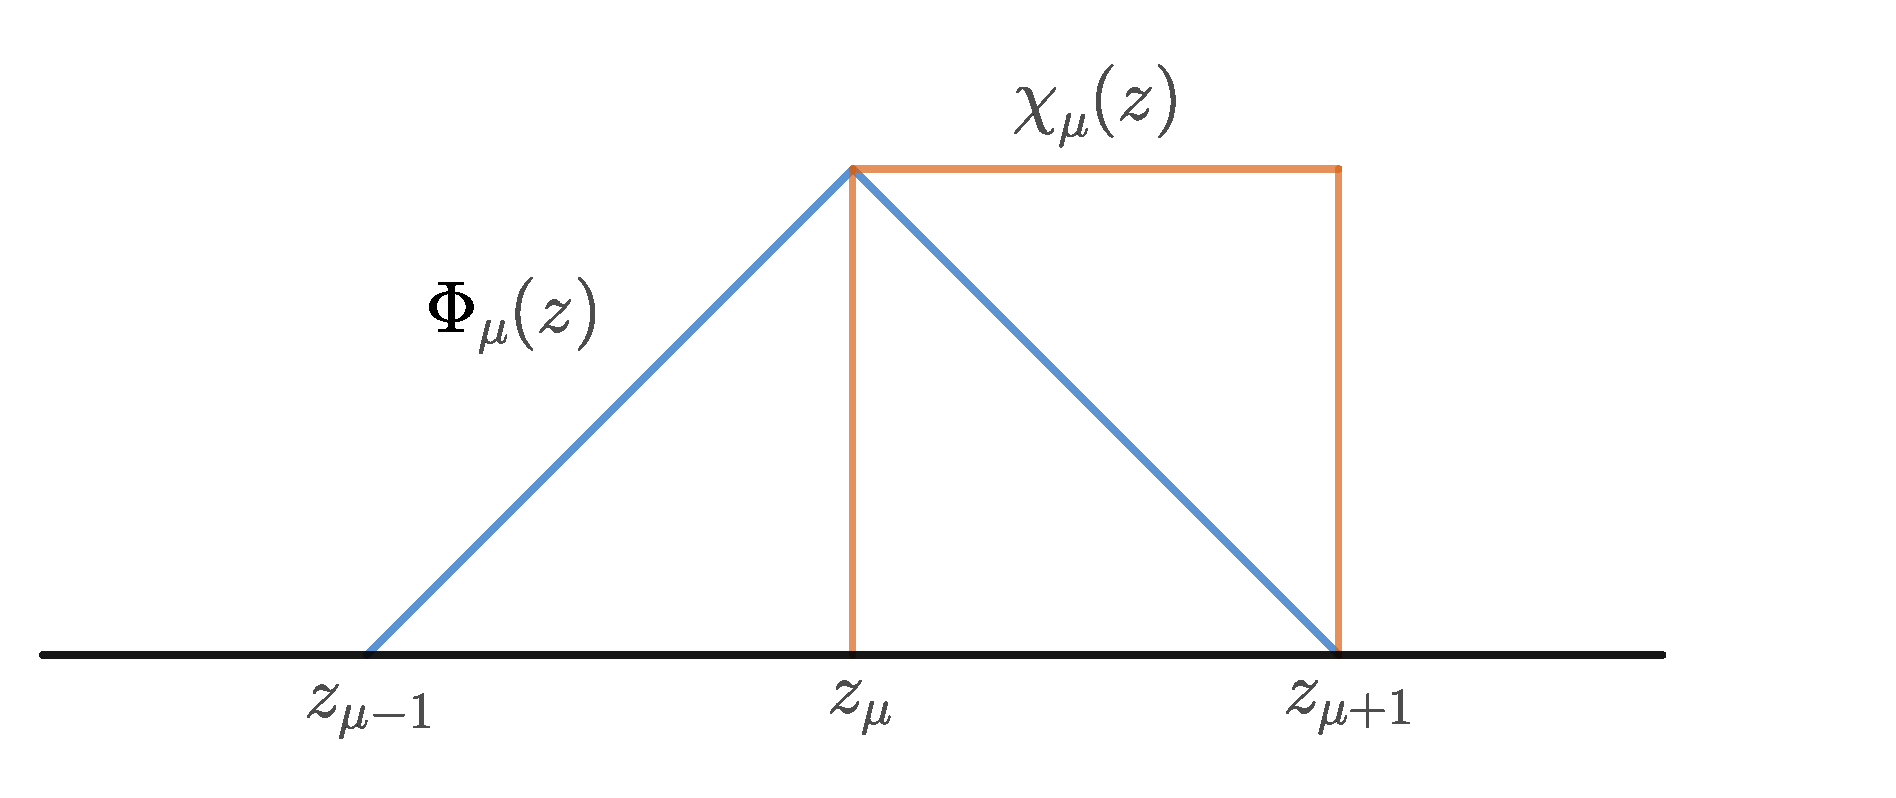
\includegraphics[scale=0.25]{psichi}
\caption{The basis function $\Phi_\mu(z)$ of node $\mu$ (blue) and the characteristic function $\chi_\mu(z)$ of bin $\mu$ (orange).}
\label{psichi}
\end{figure}

The gradient of the basis function is
\begin{align}
\boldsymbol{\nabla}\Phi_\mu({\bf r})&=-\frac{\chi_\mu({\bf r})-\chi_{\mu-1}({\bf r})}{\Delta z}{\bf n},
\label{partialpsi}
\end{align}
where ${\bf n}$ is the unit vector in the normal direction.

Following  Ref. \cite{EspanolDonev2015},  we  now introduce  dual basis  functions
$\delta_\mu({\bf  r})$ and  $\psi_\mu({\bf r})$.   The basis  function
$\delta_\mu({\bf r})$ is used to  discretize a continuum field $v({\bf
  r})$ by defining the discrete values $v_\mu$ according to
\begin{align}
  v_\mu&=\int d{\bf r}v({\bf r})\delta_\mu({\bf r})
\label{Disc}
\end{align}
On the other hand,  the  basis function  $\psi_\mu({\bf r})$ allows one
to construct a continuum field out of a discrete set of values through
interpolation, that is,
\begin{align}
    \overline{v}({\bf r}) &=\sum_{\mu}v_\mu\psi_\mu({\bf r})
\label{Cont}
\end{align}
In this chapter, overlined fields indicate  fields interpolated from
a set of discrete values. 
The basis functions are required to
satisfy the biorthonormality condition
\begin{align}
  \int d{\bf r}\delta_\mu({\bf r})\psi_\nu({\bf r})=\delta_{\mu\nu}
\label{biortho}
\end{align}
where $\delta_{\mu\nu}$ is the Kronecker delta. 
It proves convenient to introduce the following 
parenthetical notation for space integrals
\begin{align}
  \llg \cdots\rlg &=\int d{\bf r}\cdots
\label{notation}
\end{align}
and the biorthonormality condition (\ref{biortho}) becomes
\begin{align}
\llg\delta_\mu\psi_\nu\rlg=\delta_{\mu\nu}
\label{biortho2}
\end{align}
We stipulate that the relation between both basis function is linear
\begin{align}
    \delta_\mu({\bf r})=\sum_\nu M^\delta_{\mu\nu}\psi_\nu({\bf r}),&&
  \psi_\mu({\bf r})=\sum_\nu M^\psi_{\mu\nu}\delta_\nu({\bf r})
\label{dual}
\end{align}
and, then, the biorthonormality condition (\ref{biortho}) implies that 
the matrices are given by
\begin{align}
    M^\delta_{\mu\nu}= \llg\delta_\mu\delta_\nu\rlg, &&
  M^\psi_{\mu\nu}= \llg\psi_\mu\psi_\nu\rlg
\label{MM}
\end{align}
and these two matrices are inverse of each other.

The biorthonormality  condition ensures the consistency  property that
if  we  discretize  as  in (\ref{Disc})  an  interpolated  field  like
(\ref{Cont}) we get
\begin{align}
  c_\mu&=\int d{\bf r}\delta_\mu({\bf r})\overline{c}({\bf r})
=\sum_\nu\int d{\bf r}\delta_\mu({\bf r})\psi_\nu({\bf r})c_\nu=c_\mu
\end{align}
Therefore,  the   discretization  of   an  interpolated   field  gives
consistently back the original discrete field, and no errors are accumulated in the process.

Let us now specify the actual form of the basis functions.  The finite
element basis  function $\Phi_\mu({\bf  r})$ has an  associated volume
${\cal V}_\mu$ defined as
\begin{align}
  {\cal V}_{\mu}&=\int d{\bf r}\Phi_\mu({\bf r})
\end{align}
and the usual mass matrix of the finite element method is 
\begin{align}
M^\Phi_{\mu\nu}&=\llg\Phi_\mu\Phi_\nu\rlg  
\label{Mphi}
\end{align}
 and has dimensions of volume. This matrix satisfies 
\begin{align}
\sum_\mu M^\Phi_{\mu\nu} &={\cal V}_\nu
\end{align}
and, by multiplying with the inverse on both sides
\begin{align}
  \sum_\mu {\cal V}_\mu \left[M^{\Phi}\right]^{-1}_{\mu\nu}&=1
\label{sumM}
\end{align}
for all $\nu$.

The discrete  Dirac $\delta$ function is  defined in terms of  the finite
element basis function according to
\begin{align}
  \delta_\mu({\bf r})\equiv\frac{\Phi_\mu({\bf r})}{{\cal V}_\mu}
\label{DelFE}
\end{align}
The matrices $M^\delta_{\mu\nu}, M^\psi_{\mu\nu}$ defined in (\ref{MM}) are related to
the mass matrix of the finite element basis (\ref{Mphi}) through
\begin{align}
    M^\delta_{\mu\nu}=\frac{  M^\Phi_{\mu\nu}}{{\cal V}_\mu{\cal V}_\nu}, &&
M^\psi_{\mu\nu}={\cal V}_\mu \left[M^{\Phi}\right]^{-1}_{\mu\nu}{\cal V}_\nu
\label{MdMp}
\end{align}
Given the definition (\ref{DelFE}) for the discrete Dirac $\delta$ function,  the interpolant basis function given in (\ref{dual}) takes the form
\begin{align}
  \psi_\mu({\bf r})&
  ={\cal V}_\mu \sum_\nu \left[M^{\Phi}\right]^{-1}_{\mu\nu} \Phi_\nu({\bf r})
\label{PsiFE}
\end{align}
in terms of the finite element basis function set.

\section{The  discrete hydrodynamics equations derived
with the Kawasaki-Gunton projector}
\label{Sec:derivation}
In this section, we present a derivation of the governing equations of
the  dynamics   of  the   nonequilibrium  average  of   the  discrete
hydrodynamic  variables  from first  principles,  i.e.   based on  the
projection operator  technique \cite{Grabert1982}, summarized  in Sec.
\ref{Sec:Grabert} of Chapter \ref{Chap:NESM}.   The CG variables that we
consider in this chapter are the  total Hamiltonian $\hat{H}(z)$
and the discrete mass and momentum fields, which are defined according to
\begin{align}
  \hat{\rho}_\mu&= \sum_i^Nm_i\delta_\mu({\bf q}_i), &
%\nonumber\\
\hat{\bf g}_\mu&= \sum_i^N{\bf p}_i\delta_\mu({\bf q}_i)
\label{rhogmumic}
\end{align}
The  phase  functions (\ref{rhogmumic}),  as  opposed  to  the  microscopic  functions
(\ref{CGvar}) can be  measured directly in a  MD simulation. The
continuum (\ref{CGvar}) and discrete (\ref{rhogmumic}) variables
are connected by
\begin{align}
  \hat{\rho}_\mu&= \int d{\bf r}\delta_\mu({\bf r})\hat{\rho}_{\bf r},&
%\nonumber\\
  \hat{\bf g}_\mu&=\int d{\bf r}\delta_\mu({\bf r})\hat{\bf g}_{\bf r}
\label{rhogmumiccont}
\end{align}
The  discrete mass  and momentum  densities are  defined at  the nodal
planes. We see from (\ref{rhogmumic}) that  the mass density at a node
receives a contribution of the mass of fluid molecule $i$ that depends
on  the distance  of  this  molecule to  the  nodal  plane $\mu$,  and
similarly    for   the    momentum.     The   microscopic    variables
(\ref{rhogmumic}) give,  essentially, the number of  particles and the
average velocity of the particles (per  unit volume) that happen to be
``around'' the nodal plane $\mu$.

%By the very
%selection of the  variables (\ref{rhogmumic}) as the  CG variables, we
%are  making a  strong assumption  about  the situations  in which  the
%theory may be applicable.  For  example, the resulting theory will not
%be able to describe situations in which a sound wave is propagating in
%the direction \textit{parallel} to the  walls, because such a wave has
%variations in the parallel direction that cannot be captured by the CG
%variables.  However,  it will  allow us  to discuss  sound propagation
%\textit{perpendicular}  to the  walls.   It is  expected  that the  CG
%variables (\ref{rhogmumic})  will feel the  effects of the walls  in a
%very integrated form, in which the isotropy and translation invariance
%of the  walls will be a  very good approximation.  In  that sense, for
%those situations  in which the  resulting dynamic equations  are valid
%(i.e.  parallel flow),  the assumed isotropy of the  walls is expected
%to be  valid.  
%\Note{No he encontrado la referencia de Donev.} 
%
%The  calculations presented in what follows  are very
%similar to  the ones described  in Ref. \cite{Donev}, except  that the
%present  calculation  deals  with ``canonical''  averages  instead  of
%``microcanonical''  averages  as  in   Ref.  \cite{Donev}.  They  also
%crucially  differ in  that  the present  derivation  accounts for  the
%presence of confining walls.

No macroscopic variables are assumed  for the solid, because we assume
that it  is a very massive  wall with definite location.   By the very
selection of the  variables (\ref{rhogmumic}) as the  CG variables, we
are  making a  strong assumption  about  the situations  in which  the
theory may be applicable.  For  example, the resulting theory will not
be able to describe situations in which a sound wave is propagating in
the direction \textit{parallel} to the  walls, because such a wave has
variations in the parallel direction that cannot be captured by the CG
variables.  However,  it will  allow us  to discuss  sound propagation
\textit{perpendicular}  to the  walls.   It is  expected  that the  CG
variables (\ref{rhogmumic})  will feel the  effects of the walls  in a
very integrated form, in which the isotropy and translation invariance
of the  walls will be a  very good approximation.  In  that sense, for
those situations  in which the  resulting dynamic equations  are valid
(i.e.  parallel flow),  the assumed isotropy of the  walls is expected
to be  valid.  The  calculations presented in what follows  are very
similar to  the ones described  in Ref. \cite{Donev}, except  that the
present  calculation  deals  with ``canonical''  averages  instead  of
``microcanonical''  averages.  They  also
crucially  differ in  that  the present  derivation  accounts for  the
presence of confining walls.

\subsection{The time derivatives}
The time derivatives  of the CG variables  (\ref{rhogmumic}) are given
through the action of the Liouville operator
\begin{align}
  i{\cal L}  \hat{\rho}_{\mu}&=\sum_{i=1}^N{\bf p}_i\esc\boldsymbol{\nabla}\delta_\mu({\bf q}_i),&
%\nonumber\\
i{\cal L}  \hat{\bf g}_{\mu}&=\sum_{i=1}^N{\bf p}_i{\bf v}_i\esc\boldsymbol{\nabla}\delta_\mu({\bf q}_i)
+\hat{\bf F}_\mu
\label{iLMicrhogmu}
\end{align}
In the expression (\ref{iLMicrhogmu}) we see that the momentum density
changes through two different mechanism,  the convective motion of the
particles and  the forces on  the particles.  The total  force density
$\hat{\bf F}_\mu$ felt by the fluid particles at node $\mu$ is
\begin{align}
\hat{\bf F}_\mu&=    \hat{\bf F}^{\rm s\to l}_\mu+  \hat{\bf F}^{\rm l\to l}_\mu
\end{align}
where $  \hat{\bf F}^{\rm  s\to l}_\mu$  is the  force density  on the
fluid  at node  $\mu$ due  to the  solid and  $ \hat{\bf  F}^{\rm l\to
  l}_\mu$ is the force  density on the fluid at node  $\mu$ due to the
fluid. These forces are defined as
\begin{align}
    \hat{\bf F}^{\rm s\to l}_\mu \equiv\sum_{ij'}\hat{\bf F}_{ij'}\delta_\mu({\bf q}_i), &&
 \hat{\bf F}^{\rm l\to l}_\mu \equiv\sum_{ij}\hat{\bf F}_{ij}\delta_\mu({\bf q}_i)
\label{Fbin}
\end{align}
Recall that solid atoms have  primed indices and fluid atoms have unprimed indices.


For future reference,  we express the time derivative  of the discrete
momentum density field  in terms of a discrete stress  tensor. 
The  gradient   of  the  discrete   delta  function  is   given,  from
(\ref{partialpsi}) and (\ref{DelFE}), by
\begin{align}
  \boldsymbol{\nabla}\delta_\mu({\bf r})=-\frac{1}{{\cal V}_\mu}\frac{\chi_\mu(z)-\chi_{\mu-1}(z)}{\Delta z} {\bf n}
\end{align}
This means that the convective part can be expressed in the form
\begin{align}
  \sum_{i=1}^N{\bf p}_i{\bf v}_i\esc\boldsymbol{\nabla}\delta_\mu({\bf q}_i)&=
-\frac{1}{{\cal V}_\mu} \sum_{i=1}^N{\bf p}_i{\bf v}_i\esc{\bf n}\frac{\chi_\mu(z)-\chi_{\mu-1}(z)}{\Delta z}
\nonumber\\ 
\end{align}
For the force due to the fluid we may use the trick
\begin{align}
  \hat{{\bf F}}_\mu^{\rm l\to l}&=  \sum_{ij}^N\hat{\bf F}_{ij}\delta_\mu({\bf q}_i)
=\frac{1}{2}\sum_{ij}^N\hat{\bf F}_{ij}
(\delta_\mu({\bf q}_i)-\delta_\mu({\bf q}_j))
=\frac{1}{2}\sum_{ij}^N\hat{\bf F}_{ij}\int_0^1d\epsilon \frac{d}{d\epsilon}
\delta_\mu({\bf q}_j+\epsilon{\bf q}_{ij})
\nonumber\\
&=\frac{1}{2}\sum_{ij}^N\hat{\bf F}_{ij}{\bf q}_{ij}\esc\int_0^1d\epsilon 
\boldsymbol{\nabla}\delta_\mu({\bf q}_j+\epsilon{\bf q}_{ij})
\end{align}
Therefore we have
\begin{align}
   \sum_{ij}^N\hat{\bf F}_{ij}\delta_\mu({\bf q}_i)
   &=\frac{1}{2}\sum_{ij}^N\hat{\bf F}_{ij}{\bf q}_{ij}\esc{\bf n}
   %\nonumber\\
%\times
\int_0^1d\epsilon 
\frac{1}{{\cal V}_\mu}\frac{\chi_\mu({\bf q}_j+\epsilon{\bf q}_{ij})-\chi_{\mu-1}({\bf q}_j+\epsilon{\bf q}_{ij})}{\Delta z} 
\nonumber\\
& 
=\frac{1}{{\cal V}_\mu}\frac{1}{2}\sum_{ij}^N\hat{\bf F}_{ij}{\bf q}_{ij}\esc{\bf n}
\frac{z_\mu(i,j)-z_{\mu-1}(i,j)}{\Delta z} 
\label{Fvir}
\end{align}
where we have introduced the geometric factor 
\begin{align}
z_\mu(i,j)&=  \int_0^{1}d\epsilon\chi_\mu({\bf q}_i-\epsilon{\bf q}_{ij})
\nonumber\\
&=  \int_0^{1}d\epsilon
\theta(z_{\mu+1}-z_i+\epsilon z_{ij})\theta(z_i-\epsilon z_{ij}-z_\mu)
\nonumber\\
&= \frac{1}{z_{ij}} \int_0^{z_{ij}}dz
\theta(z_{\mu+1}-z_i+z)\theta(z_i-z_\mu-z)
\label{int}
\end{align}
The integral can be easily computed with the result
\begin{align}
 z_\mu(i,j)=&\frac{1}{z_{ij}}\left[(z_j-z_\mu) \theta(z_{\mu+1}-z_{j},z_\mu-z_{j} )\right.
%\nonumber\\
-(z_i-z_\mu) \theta(z_{\mu+1}-z_i,z_\mu-z_i)
\nonumber\\
&-(z_{j}-z_{\mu+1}) \theta(z_{\mu+1}-z_{j})
%\nonumber\\
\left.+(z_i-z_{\mu+1}) \theta (z_{\mu+1}-z_i)\right],
\label{geoFactor}
\end{align}
where  $\theta(a,b)=\theta(a)\theta(b)$  takes  the value  1  if  both
$a,b>0$, and  zero otherwise.  Note that  $z_\mu(i,j)=z_\mu(j,i)$.  If
both particles are within the bin,  then $ z_\mu(i,j)=1$.  If the line
joining  the   particles  does  not   cross  the  bin   (for  example,
$z_i,z_j<z_\mu$) then  $z_\mu(i,j)=0$.  If both particles  are outside
the  bin, but  the line  joining the  particles crosses  the bin  (for
example,                $z_i<z_\mu,z_j>z_{\mu+1}$)                then
$z_\mu(i,j)=\frac{z_{\mu+1}-z_\mu}{z_j-z_i}$. Finally, if one particle
is   in    the   bin,   and    the   other   outside    (for   example
$z_\mu<z_i<z_{\mu+1},               z_j>z_{\mu+1}$)               then
$z_\mu(i,j)=\frac{z_{\mu+1}-z_i}{z_j-z_i}$.  In  summary, $z_\mu(i,j)$
is  the fraction  of  the segment  of  the \textit{vertical}  distance
between particles $i,j$ that happens to  be within the bin $\mu$. 
%Note that by Thale's theorem this fraction  is equal to the fraction of the \textit{length} of the segment joining particles $i,j$ that happens to be  inside  the bin.  
The  partition  of unity  (\ref{PartitionUnity})
implies also that
\begin{align}
  \sum_\mu z_{\mu}(i,j) =1,
\label{zmu1}
\end{align}
as can be seen easily from the definition (\ref{int}).

By                collecting                the                results
(\ref{iLMicrhogmu}),(\ref{Fbin}),(\ref{Fvir}) we end  up
with the final form of the time derivative of the discrete momentum variable
\begin{align}
  i{\cal L}\hat{\bf g}_\mu &=\hat{\bf F}_\mu^{\rm s\to l}-\frac{\hat{\boldsymbol{\sigma}}_\mu-\hat{\boldsymbol{\sigma}}_{\mu-1}}{\Delta z}\esc{\bf n},
\label{equationivalence}
\end{align}
where we have introduced the discrete stress tensor of bin $\mu$ through
\begin{align}
 \hat{ \boldsymbol{\sigma}}_{\mu}
% &=\hat{\bf K}_\mu+\hat{\boldsymbol{\Pi}}_{\mu}
% \nonumber\\
&=
\frac{1}{{\cal V}_\mu} \left[\sum_i{\bf p}_i{\bf v}_i\chi_\mu({\bf r}_i)
+\frac{1}{2}\sum^{N}_{ij}{\bf r}_{ij}\hat{\bf F}_{ij}z_\mu(i,j)\right]
\label{sbin}
\end{align}
The form of  equation (\ref{equationivalence}) makes explicit  that the momentum
density changes due to the force density due to the solid wall and the
discrete gradient of  the fluid stress tensor. As shown in Chapter \ref{Chap:Theory}, this  separation of the
force on the fluid into  solid-fluid and fluid-fluid interactions is at
the basis of the final structure of the hydrodynamic equations.

Note  that, while  the force  is discretized  with the  basis function
$\Phi_\mu({\bf r})$, the stress is discretized with the characteristic
function $\chi_\mu({\bf  r})$. Therefore, forces are  defined on nodal
planes    while    stresses    are    defined    on    bins.     
%Refs.
%\cite{Schindler2010,Lion2012} have  considered the definition  of local
%pressure following similar lines.


The partitions  of unity (\ref{PartitionUnity}) and  (\ref{zmu1}) ensure
that the arithmetic average of the stress tensor of the bins gives the
total stress tensor of the system, that is,
\begin{align}
\frac{1}{N_{\rm bin}}\sum_{\mu}^{N_{\rm bin}}\hat{\boldsymbol{\sigma}}_{\mu}=\hat{\boldsymbol{\sigma}},
\end{align}
where the total fluid stress tensor of the system is defined in the usual way as
\begin{align}
  \hat{\boldsymbol{\sigma}}=\frac{1}{V}\left[\sum_{i}{\bf p}_i{\bf v}_i
+\frac{1}{2}\sum_{ij}{\bf r}_{ij}\hat{\bf F}_{ij}\right]
\end{align}
and the total volume of the system is $V=L_xL_yL_z$.

\subsection{Exact reversible part of the dynamics}
As shown in Sec. \ref{Sec:ExactCont} of Chapter \ref{Chap:Theory} , the reversible part
of  the dynamics  is  given by  the average  of  the microscopic  time
derivatives with respect to the  relevant ensemble.  The explicit form
of the relevant ensemble and the corresponding averages leading to the
reversible  part   of  the   dynamics  are   given  in   the  Appendix
\ref{Ap:KG}.  There  it is  shown  that  the  reversible part  of  the
dynamics is given by the \textit{exact} equations
\begin{align}
  \llangle i{\cal L}\hat{\rho}_\mu\rrangle^{\lambda{\bf v}} &=
  \llg\llangle \hat{\rho}_{\bf r}\rrangle^{\lambda{\bf v}}
\overline{\bf v}\esc\boldsymbol{\nabla}\delta_{\mu}\rlg
\nonumber\\
  \llangle i{\cal L}\hat{\bf g}_\mu\rrangle^{\lambda{\bf v}} &=
\llg\llangle \hat{\rho}_{\bf r}\rrangle^{\lambda{\bf v}}
\overline{\bf v}\overline{\bf v}\esc\boldsymbol{\nabla}\delta_{\mu}\rlg
+\llg\delta_\mu\llangle\hat{\rho}_{\bf r}\rrangle^{\lambda{\bf v}}\boldsymbol{\nabla}\overline{\mu}\rlg,
\label{ExactRev}
\end{align}
where we have used the  notation (\ref{notation}) for space integrals,
the  notation  (\ref{Cont})  for interpolated  fields,  and  $\llangle
\hat{\rho}_{\bf  r}\rrangle^{\lambda{\bf v}}$  is the  average of  the
microscopic  density field  (\ref{CGvar})  with  respect to  the
relevant  ensemble.  The  chemical potential  field per  unit mass  is
defined by
\begin{align}
  \overline{\mu}({\bf r})&=\overline{\lambda}({\bf r})-\frac{\overline{\bf v}^2({\bf r})}{2}
\end{align}
where the interpolated conjugate variables are defined as 
\begin{align}
    \overline{\lambda}({\bf r})=\sum_{\mu}{\lambda}_{\mu}\psi_\mu({\bf r}), &&
\overline{\bf v}({\bf r})=\sum_{\mu}{\bf v}_{\mu}\psi_\mu({\bf r})
\end{align}
The conjugate variables $\lambda_\mu,{\bf v}_\mu$ are functions of the
CG variables averages $\rho_\mu,{\bf g}_\mu$, computed with the real ensemble (i.e. the solution of the Liouville equation). In particular, the velocity ${\bf
v}_\mu$ is related to the momentum density through
\begin{align}
  {\bf g}_\mu&=\sum_{\nu}\rho_{\mu\nu}{\bf v}_\nu
\label{vnu}
\end{align}
where  the mass density matrix is defined by
\begin{align}
  \rho_{\mu\nu} =\int d{\bf r}
\delta_\mu({\bf r})\psi_\nu({\bf r})\llangle\hat{\rho}_{\bf r}\rrangle^{\lambda{\bf v}}
\label{rhomunu}
\end{align}

\subsection{Approximate reversible dynamics}
The reversible part  of the dynamics (\ref{ExactRev}) is  not given in
\textit{explicit} form in terms of the discrete CG variables, that are
hidden inside  the Lagrange multipliers $\lambda_\mu,{\bf  v}_\mu$ and
the  average $\llangle  \hat{\rho}_{\bf r}\rrangle^{\lambda{\bf  v}}$.
We consider  now an approximation  that will make the  exact equations
(\ref{ExactRev}) explicit in the CG variables.  This approximation has
been named  as the \textit{linear  for spiky approximation}  (LFSA) in
Ref.   \cite{Donev},  and  consists on  approximating,  within  ensemble
averages,  the ``spiky''  fields (\ref{rhogmumic})  with piece-wise
linear functions as 
\begin{align}
  \hat{\rho}_{\bf r}&\simeq \sum_\sigma\hat{\rho}_{\sigma} \psi_\sigma({\bf r})
\nonumber\\
  \hat{\bf g}_{\bf r} &\simeq \sum_\sigma\hat{\bf g}_{\sigma} \psi_\sigma({\bf r})
\label{LFSA}
\end{align}
\begin{figure}
    \centering
    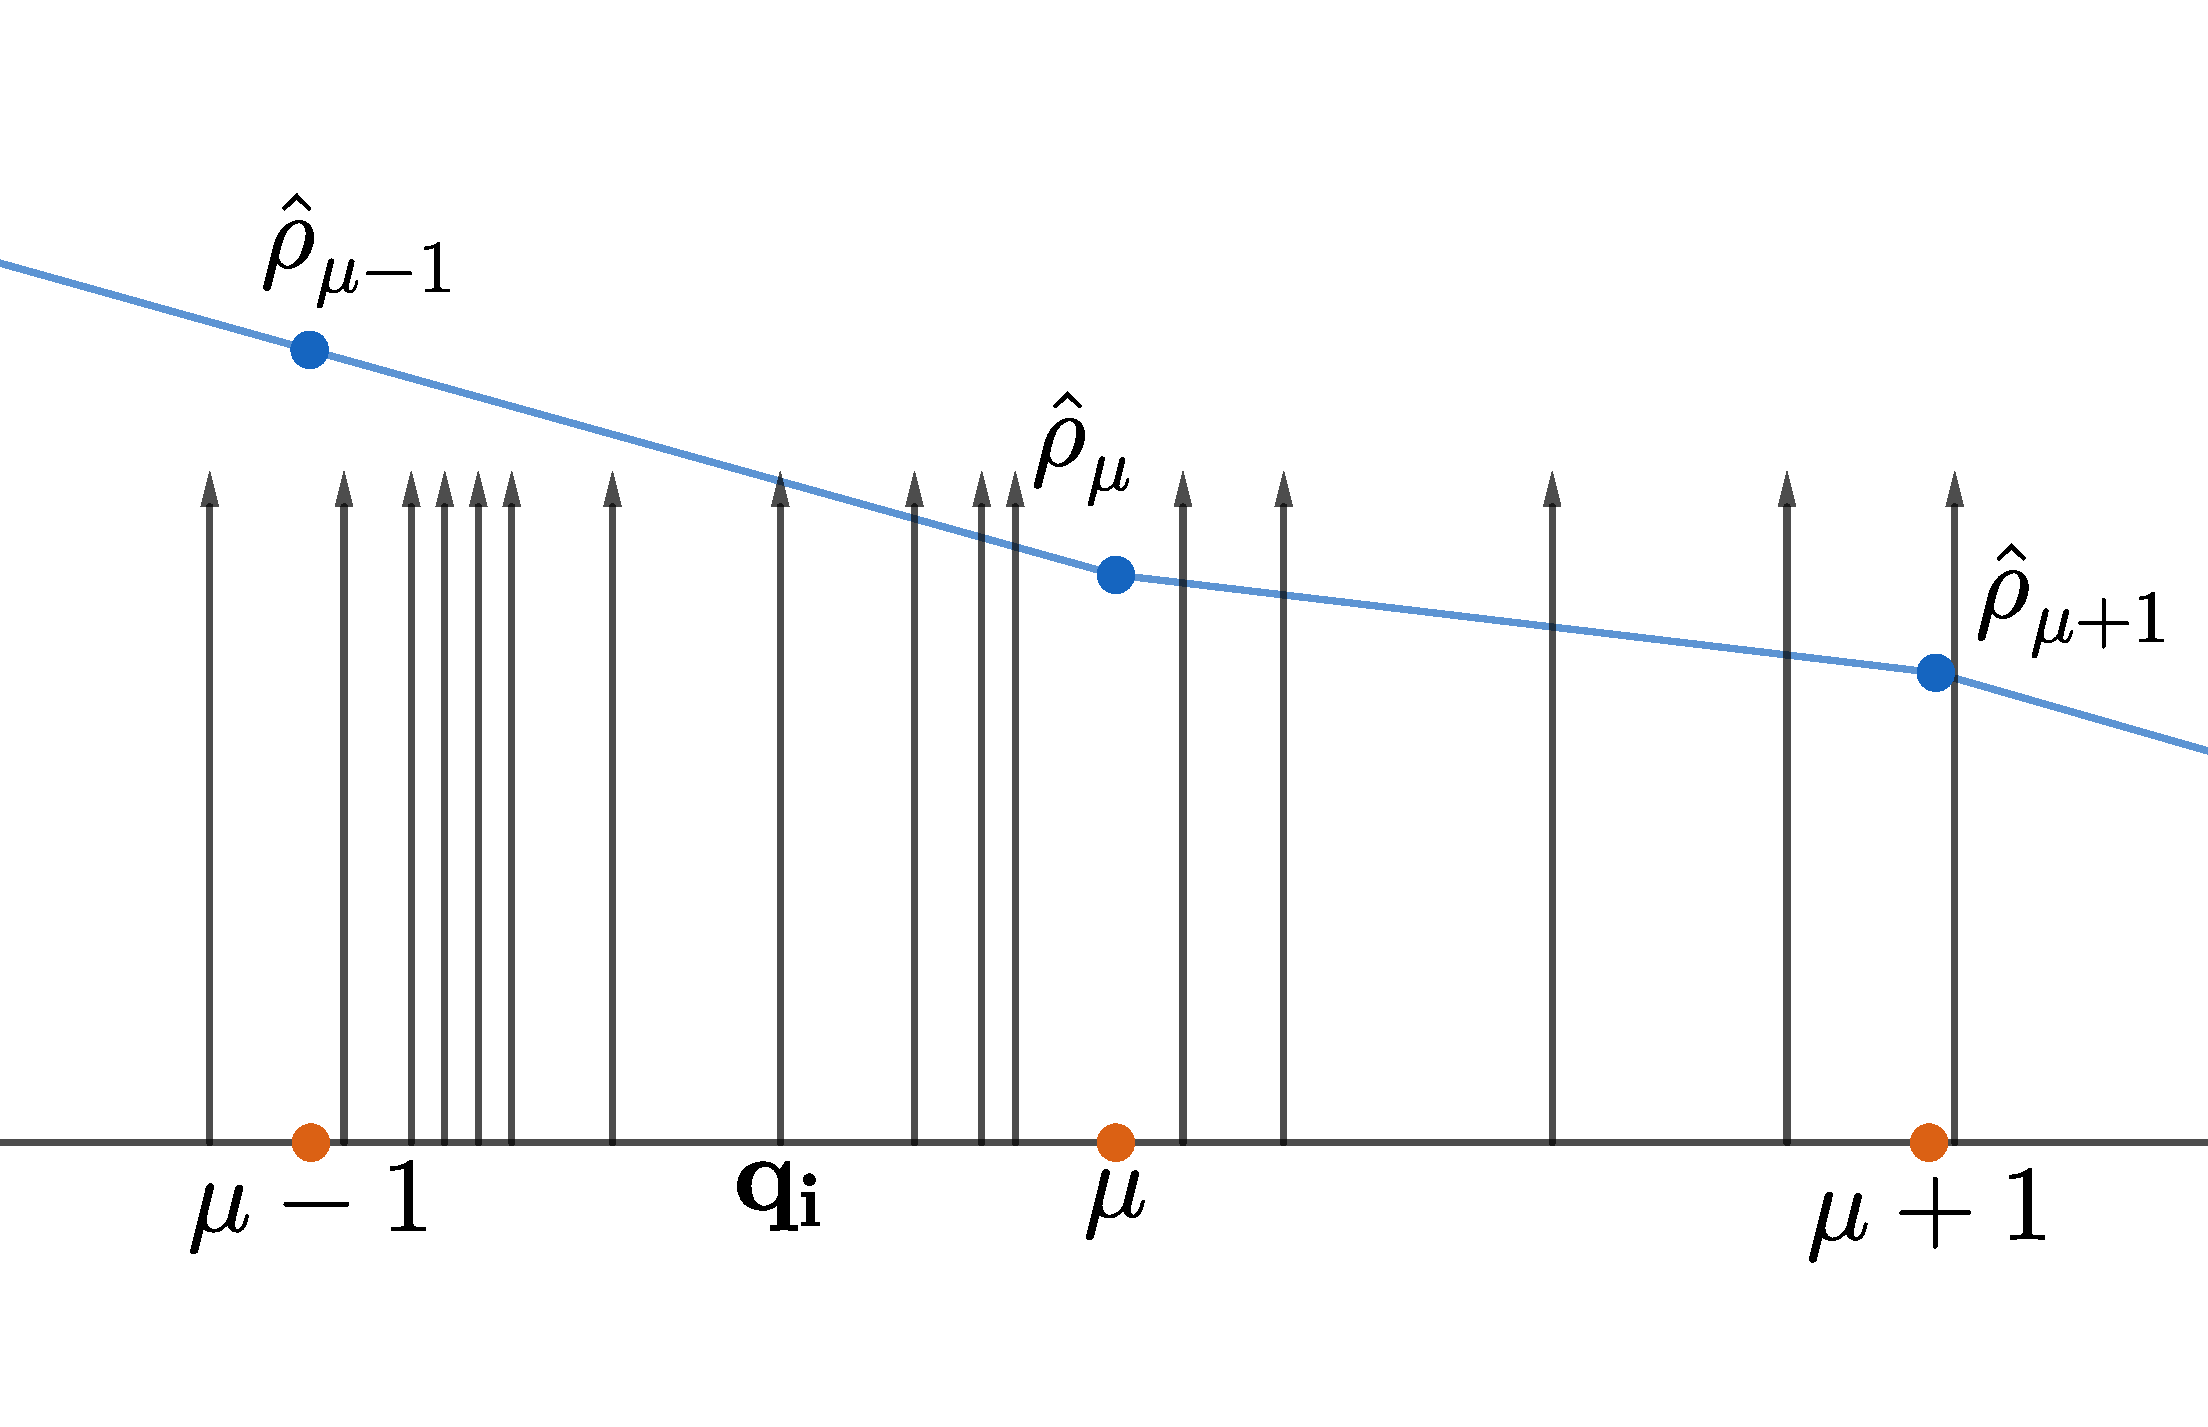
\includegraphics[scale=0.2]{spiky}
    \caption[``Spiky'' aproximation]{The microscopic density field $\hat{\rho}_{\bf r}{\bf}(z)$ (black), which is a sum of Dirac $\delta$ functions each one located at the position of the particle $i$, is approximated by an interpolation of the discrete microscopic density field $\hat{\rho}_{\mu}(z)$ at the nodes (blue).}
    \label{fig:spiky}
\end{figure}
As illustrated in Fig. (\ref{fig:spiky}), the left  hand side contains  sums of singular Dirac  $\delta$ functions,
while the  right hand  side are piece-wise  linear functions  given in
terms   of   the  discrete   values   $\hat{\rho}_{\sigma} ,\hat{\bf
  g}_\sigma $.   This  approximation  is  expected  to  hold  inside
ensemble averages and to be a good one if there are many particles per
bin. 

In the LFSA, the average of the density field becomes explicit
in the discrete density variables
\begin{align}
  \llangle \hat{\rho}_{\bf r}\rrangle^{\lambda{\bf v}}&\simeq
\sum_\mu\rho_\mu\psi_\mu({\bf r})=\overline{\rho}({\bf r})
\end{align}
and the density matrix (\ref{rhomunu}) becomes explicit in the discrete density 
\begin{align}
  \rho_{\mu\nu} \simeq \sum_\sigma\llg\delta_\mu\psi_\nu\psi_\sigma\rlg\rho_\sigma
=\llg\delta_\mu\psi_\nu\overline{\rho}\rlg
\label{calR1}
\end{align}
Therefore, the discrete velocity  field (\ref{vnu}) is given explicitly
in terms of the discrete mass and momentum densities by
\begin{align}
{\bf v}_\mu&=\sum_\nu\rho^{-1}_{\mu\nu}{\bf g}_\nu
\label{un}
\end{align}

Under this  LFSA the reversible  part (\ref{ExactRev}) takes
the \textit{explicit} form
\begin{align}
  \llangle i{\cal L}  \hat{\rho}_{\mu}\rrangle^{\lambda{\bf v}}&= 
\llg \overline{\rho}\;\overline{\bf v}\esc\boldsymbol{\nabla}\delta_\mu\rlg
\nonumber\\
\llangle i{\cal L}  \hat{\bf g}_{\mu}\rrangle^{\lambda{\bf v}} &=
\llg\overline{\rho}\;\overline{\bf v}\;\overline{\bf v}\esc\boldsymbol{\nabla}\delta_{\mu}\rlg
+\llg\delta_\mu\overline{\rho}\boldsymbol{\nabla}\overline{\mu}\rlg
\label{RevDis0}
\end{align}
These equations  are explicit in  the CG variables because  the fields
$\overline{\rho}({\bf  r}),\overline{\bf  v}({\bf  r})$  are  explicit
functions  of the  discrete CG  variables $\rho_\mu,{\bf  v}_\mu$.  As
shown  in  the  Appendix  \ref{Ap:KG}, the  last  term  involving  the
chemical potential admits the following form
\begin{align}
  \llg\delta_\mu\overline{\rho}\boldsymbol{\nabla}\overline{\mu}\rlg&=
-\sum_\nu\llg\overline{\rho}\delta_{\mu}\boldsymbol{\nabla}\delta_{\nu}\rlg
\frac{\partial  F}{\partial \rho_{\nu}}(\rho),
\end{align}
where the free energy function depends only on the discrete density field.

Therefore, the final reversible part of the dynamics takes the form 
\begin{align}
  \llangle i{\cal L}  \hat{\rho}_{\mu}\rrangle^{\lambda{\bf v}}&= 
\llg \overline{\rho}\;\overline{\bf v}\esc\boldsymbol{\nabla}\delta_\mu\rlg
\nonumber\\
\llangle i{\cal L}  \hat{\bf g}_{\mu}\rrangle^{\lambda{\bf v}} &=
\llg\overline{\rho}\;\overline{\bf v}\;\overline{\bf v}\esc\boldsymbol{\nabla}\delta_{\mu}\rlg
-\sum_\nu\llg\overline{\rho}\delta_{\mu}\boldsymbol{\nabla}\delta_{\nu}\rlg
\frac{\partial  F}{\partial \rho_{\nu}}(\rho)
\label{RevDis}
\end{align}

\subsection{Irreversible part of the dynamics}
As shown in  Sec. \ref{Sec:Grabert} of Chapter  \ref{Chap:NESM}, the  irreversible part of the
dynamics in  the projection operator  method is given by  the standard
form
\begin{align}
  \sum_jD_{ij}\frac{\partial S}{\partial a_j},
\label{IrrDis0}
\end{align}
where $S$ is the entropy and the dissipative matrix is given by
\begin{align}
  D_{ij}=\frac{1}{k_BT}\int_0^\tau\llangle {\cal Q}i{\cal L}\hat{A}_i(t){\cal Q}i{\cal L}\hat{A}_j\rrangle^{\lambda}
\end{align}
%where $\llangle\cdots\rrangle^\lambda$  is an  average taken  with the relevant  ensemble.
Therefore,  the dissipative  matrix  depends,  in
general, on the state of the CG variables.  In the present case, the CG
variables are $\hat{\rho}_\mu$ and $\hat{\bf g}_\mu$.   In the
LFSA (\ref{LFSA}) the time derivative of the density is given by
\begin{align}
  i{\cal L}\hat{\rho}_\mu &=\int d{\bf r}\hat{\bf g}_{\bf r} \esc\boldsymbol{\nabla}\delta_\mu({\bf r})
\simeq \sum_\nu\hat{\bf g}_\nu \llg\psi_\nu\boldsymbol{\nabla}\delta_\mu\rlg
\end{align}
We see  that this time  derivative is given  in terms of  the discrete
momentum which is a CG  variable itself and, therefore, the associated
projected  current vanishes,  ${\cal Q}i{\cal  L}\hat{\rho}_\mu =0$.
This leads to a much simpler dissipative matrix.
% \footnote{In  this  approximation  we are  assuming  that  the
%   Brenner diffusion coefficients are  negligibly small}. 
The derivatives of the entropy are  given in equations  (\ref{derS}) in the
Appendix \ref{Ap:KG}, and we  may write the irreversible  terms (\ref{IrrDis0}) in
the form
\begin{align}
\left.\frac{d}{dt}\left(\begin{array}{c}
\rho_\mu\\
{\bf g}_\mu
\end{array}\right)\right|_{\rm irr}
&=\sum_\nu\left(\begin{array}{cc}
0&0\\
0&{\bf D}_{\mu\nu}
\end{array}\right)\left(
\begin{array}{c}
{\cal V}_\nu \tilde{\lambda}_\nu\\
-{\cal V}_\nu \tilde{\bf v}_\nu
\end{array}\right), 
\label{IrrDis}
\end{align}
where the dissipative matrix is given by
\begin{align}
{\bf D}_{\mu\nu}&=  \frac{1}{k_BT}
\int_0^\tau dt \llangle {\cal Q}i{\cal L}\hat{\bf g}_\mu(t){\cal Q}i{\cal L}\hat{\bf g}_\nu\rrangle^{\lambda{\bf v}} 
\label{Dmunu}
\end{align}
and we have introduced the discrete fields
\begin{align}
    \tilde{\lambda}_\mu=\sum_\nu{\cal V}_{\nu}\left[M^\Phi\right]^{-1}_{\mu\nu}\lambda_{\nu}, &&
\tilde{\bf v}_\mu=\sum_\nu{\cal V}_{\nu}\left[M^\Phi\right]^{-1}_{\mu\nu}{\bf v}_{\nu}
\label{overlined}
\end{align}
% These quantities $ \tilde{\rho}_\mu, \tilde{\bf v}_\mu$
% are  a  smoothed  representation  of the  original  discrete  CG
% variables $\rho_{\mu} {\bf v}_{\mu}$.

By  using  now  the  decomposition  (\ref{equationivalence})  of  the  time
derivative  of   the  momentum  density  in   the  dissipative  matrix
(\ref{Dmunu}),  we  obtain  the  following irreversible  part  of  the
dynamics
\begin{align}
  \left.\frac{d}{dt}\rho_\mu\right|_{\rm irr}=& 0
\nonumber\\
\left.\frac{d}{dt}{\bf g}_\mu\right|_{\rm irr}=
%\nonumber\\
&-\sum_{\nu}{\cal V}_\nu \frac{{\bf n}\esc\left[\boldsymbol{\eta}_{\mu\nu}-\boldsymbol{\eta}_{\mu-1\nu}-\boldsymbol{\eta}_{\mu\nu-1}+\boldsymbol{\eta}_{\mu-1\nu-1}\right]}{\Delta z^2}:{\bf n}\tilde{\bf v}_\nu
\nonumber\\
&+\sum_{\nu}{\cal V}_\nu\frac{\left[{\bf G}_{\mu\nu}-{\bf G}_{\mu\nu-1}\right]}{\Delta z}\esc{\bf n}\tilde{\bf v}_\nu
\nonumber\\
&+\sum_{\nu}{\cal V}_\nu\frac{{\bf n}\esc\left[{\bf H}_{\mu\nu}-{\bf H}_{\mu-1\nu}\right]}{\Delta z}\esc\tilde{\bf v}_\nu
\nonumber\\
&-\sum_{\nu}{\cal V}_\nu\boldsymbol{\gamma}_{\mu\nu}\esc\tilde{\bf v}_\nu,
\label{Irr-Fin}
\end{align}
where we have introduced the following tensorial transport matrices
\begin{align}
\boldsymbol{\eta}_{\mu\nu}
&=\frac{1}{k_BT}\int_0^{\tau} dt
\left\langle {\cal Q}\hat{\boldsymbol{\sigma}}_{\mu}(t){\cal Q}\hat{\boldsymbol{\sigma}}_{\nu}
\right\rangle^{\lambda{\bf v}}
&&\simeq\frac{1}{k_BT}\int_0^{\tau} dt
\left\langle {\cal Q}\hat{\boldsymbol{\sigma}}_{\mu}(t){\cal Q}\hat{\boldsymbol{\sigma}}_{\nu}
\right\rangle
\nonumber\\
{\bf G}_{\mu\nu}
&=\frac{1}{k_BT}\int_0^{\tau} dt
\left\langle{\cal Q}\hat{\bf F}^{\rm s\to l}_\mu(t)
{\cal Q}\hat{\boldsymbol{\sigma}}_\nu
\right\rangle^{\lambda{\bf v}}
&&\simeq\frac{1}{k_BT}\int_0^{\tau} dt
\left\langle{\cal Q}\hat{\bf F}^{\rm s\to l}_\mu(t)
{\cal Q}\hat{\boldsymbol{\sigma}}_\nu
\right\rangle
\nonumber\\
{\bf H}_{\mu\nu}&=
\frac{1}{k_BT}\int_0^{\tau} dt
\left\langle{\cal Q}\hat{\boldsymbol{\sigma}}_\mu(t){\cal Q}\hat{\bf F}^{\rm s\to l}_\nu\right\rangle^{\lambda{\bf v}}
&&\simeq\frac{1}{k_BT}\int_0^{\tau} dt
\left\langle{\cal Q}\hat{\boldsymbol{\sigma}}_\mu(t){\cal Q}\hat{\bf F}^{\rm s\to l}_\nu\right\rangle
\nonumber\\
\boldsymbol{\gamma}_{\mu\nu}
&=\frac{1}{k_BT}\int_0^{\tau} dt
\left\langle 
{\cal Q}\hat{\bf F}^{\rm s\to l}_\mu(t)
{\cal Q}\hat{\bf F}^{\rm s\to l}_\nu\right\rangle^{\lambda{\bf v}}
&&\simeq\frac{1}{k_BT}\int_0^{\tau} dt
\left\langle 
{\cal Q}\hat{\bf F}^{\rm s\to l}_\mu(t)
{\cal Q}\hat{\bf F}^{\rm s\to l}_\nu\right\rangle
\label{MolTransportCoeff}
\end{align}
Note that we have approximated the relevant ensemble $\llangle\cdots\rrangle^{\lambda,{\bf v}}$ by the equilibrium ensemble $\llangle\cdots\rrangle$ in the calculation of the above transport coefficientes. 
In  general, the transport coefficients
dependent on the CG state of  the system through the average with the
relevant  ensemble.   This
poses a large  complication in its actual evaluation. Assuming that  we may approximate the relevant ensemble
by the equilibrium ensemble
in  the   calculation   of  the   transport
coefficients, the
transport coefficients  do not depend  on local values of  density and
momenta.  They depend only on  the global thermodynamic point at which
the equilibrium correlations are computed.


%The  transport  kernels  (\ref{MolTransportCoeff}) are  given  through
%Green-Kubo  formulas.  The  transport  coefficients  are, in  general,
%dependent on the CG state of  the system, through the average with the
%relevant  ensemble  $\llangle\cdots\rrangle^{\lambda,{\bf v}}$.   This
%poses a large  complication in its actual evaluation.  We simply assume that  we may approximate the relevant ensemble
%$\llangle\cdots\rrangle^{\lambda,{\bf v}}$ by the equilibrium ensemble
%$\llangle\cdots\rrangle$   in  the   calculation   of  the   transport
%coefficients  in  (\ref{MolTransportCoeff}), in  such  a  way that  the
%transport coefficients  do not depend  on local values of  density and
%momenta.  They depend only on  the global thermodynamic point at which
%the equilibrium correlations are computed.

\subsection{The final discretized equations}
By   collecting  the   reversible   (\ref{RevDis})  and   irreversible
(\ref{Irr-Fin})  parts of  the dynamics  we  obtain the  final set  of
discrete equations
\begin{align}
\frac{d}{dt}\rho_\mu=&  \llg\overline{\rho} \; \overline{\bf v}\boldsymbol{\nabla}\delta_\mu \rlg
\nonumber\\
\frac{d}{dt}{\bf g}_\mu=&
\llg\overline{\rho} \overline{\bf v}\;\overline{\bf v}\esc\boldsymbol{\nabla}\delta_{\mu}\rlg
-\sum_\nu\llg\overline{\rho}\delta_{\mu}\boldsymbol{\nabla}\delta_{\nu}\rlg
\frac{\partial  F}{\partial \rho_{\nu}}(\rho)
\nonumber\\
-&\sum_{\nu}{\cal V}_\nu \frac{{\bf n}\esc\left[\boldsymbol{\eta}_{\mu\nu}-\boldsymbol{\eta}_{\mu-1\nu}-\boldsymbol{\eta}_{\mu\nu-1}+\boldsymbol{\eta}_{\mu-1\nu-1}\right]}{\Delta z^2}:{\bf n}\tilde{\bf v}_\nu
\nonumber\\
+&\sum_{\nu}{\cal V}_\nu\frac{\left[{\bf G}_{\mu\nu}-{\bf G}_{\mu\nu-1}\right]}{\Delta z}\esc{\bf n}\tilde{\bf v}_\nu
\nonumber\\
+&\sum_{\nu}{\cal V}_\nu\frac{{\bf n}\esc\left[{\bf H}_{\mu\nu}-{\bf H}_{\mu-1\nu}\right]}{\Delta z}\esc\tilde{\bf v}_\nu
\nonumber\\
-&\sum_{\nu}{\cal V}_\nu\boldsymbol{\gamma}_{\mu\nu}\esc\tilde{\bf v}_\nu
\label{TheoryDiscFin}
\end{align}
% Note  that equation   (\ref{TheoryDiscFin})  contains  information about  a
% single planar wall.   In the case of two planar  walls as those needed
% in MD simulations,  we need to consider the force  density due to both
% walls, which will be of the form
% \begin{align}
% \boldsymbol{{\cal S}}^\pm_\mu
% =&+\sum_{\nu}{\cal V}_\nu\frac{\left[{\bf G}^{\pm}_{\mu\nu}-{\bf G}^{\pm}_{\mu\nu-1}\right]}{\Delta z}\esc {\bf n}\overline{\bf v}_\nu
% \nonumber\\
% &+\sum_{\nu}{\cal V}_\nu\frac{{\bf n}\esc\left[{\bf H}^{\pm}_{\mu\nu}-{\bf H}^{\pm}_{\mu-1\nu}\right]}{\Delta z}
% \esc(\overline{\bf v}_\nu-{\bf V}^\pm)
% \nonumber\\
% &-\sum_{\nu}{\cal V}_\nu\boldsymbol{\gamma}^{\pm}_{\mu\nu}\esc(\overline{\bf v}_\nu-{\bf V}^\pm)
% \label{Spm}
% \end{align}
% where  $\pm$ means  upper  or  lower wall,  which  may have  different
% velocities ${\bf V}^\pm$ in general.

% Note that  the surface  density force  $\boldsymbol{{\cal S}}^\pm_\mu$
% due  to  the  walls  contains   the  transport  kernels  that  involve
% Green-Kubo correlation  with the  microscopic force  $\hat{\bf F}^{\rm
%   s\to l}_\mu$  that the solid atoms  exert on the fluid.   Due to the
% finite range  of interaction of  the microscopic force,  the resulting
% surface force  $\boldsymbol{{\cal S}}^\pm_\mu$ is different  from zero
% only on those bins $\mu$ close to the walls that fall within the range
% of  interaction of  the microscopic  force. Its  worth noting that  the
% present discrete theory does not  require any boundary condition to be
% applied on any of the bins close to the solid. The forces on the fluid
% due to the solid are taken into account explicitly without need of any
% boundary condition.

These equations are a closed system of ordinary differential equations
that  govern the  evolution of  the discrete  variables $\rho_\mu,{\bf
  g}_\mu$. Note  that the transport  kernels (\ref{MolTransportCoeff})
contain too many  components. We consider next how  they simplify when
we assume that the walls are isotropic and traslation invariant.


\subsection{Symmetry assumptions}
We now take  advantage of the assumption that the  system is isotropic
when we rotate  it with respect to an axis  perpendicular to the walls
and reflect  it with respect  to a  plane containing the  axis.  These
symmetries reflect into an enormous simplification of the structure of
the fourth order tensor  $\boldsymbol{\eta}_{\mu\nu}$, the third order
tensors  ${\bf  G}_{\mu\nu},{\bf  H}_{\mu\nu}$ and  the  second  order
tensor  $\boldsymbol{\gamma}_{\mu\nu}$.   Camargo et al. discussed in
Ref. \cite{CamargoBC2018} what are  the most  general forms  of the
tensors                     ${\bf                     G}_{\mu\nu},{\bf
  H}_{\mu\nu},\boldsymbol{\gamma}_{\mu\nu}$  satisfying  the  required
symmetries.  In Appendix \ref{Ap:Iso} we discuss
the most general fourth order tensor $\boldsymbol{\eta}_{\mu\nu}$ with
the required  symmetries.  We  introduce normal  ${\bf n}{\bf  n}$ and
tangential  ${\bf T}=\boldsymbol{\delta}-{\bf  n}{\bf n}$  projectors, where $\boldsymbol{\delta}$ is the unit matrix. 
We note that the tangential projector satisfies
\begin{align}
{\bf  T}^{\alpha  z}=\delta^{\alpha z}-{\bf n}^\alpha{\bf n}^z=0\quad\quad \forall \alpha=x,y,z
\label{T3}
\end{align}
and, therefore, the required components of the viscosity tensor for an
isotropic wall  are given, from equation (\ref{viscosityTangential}) in the
Appendix \ref{Ap:Iso}, by
\begin{align}
  \boldsymbol{\eta}^{\alpha z\gamma z}&=  
\eta^{||} {\bf T}^{\alpha\gamma}+\eta^{\bot} {\bf n}^\alpha  {\bf n}^\gamma 
\label{etasimple}
\end{align}
The  required components  of the  third order
tensors are, from  equations (104) and (105) of Ref. \cite{CamargoBC2018}
\begin{align}
{\bf G}^{\alpha\beta z}
&=G^{||}{\bf T}^{\alpha\beta}+
G^{\bot}{\bf n}^{\alpha}{\bf n}^{\beta}
\nonumber\\
{\bf H}^{\alpha z\gamma}
&=H^{||}{\bf T}^{\alpha\gamma}+
H^{\bot}{\bf n}^{\alpha}{\bf n}^{\gamma}
\label{GH}
\end{align}
and the second order friction tensor becomes, under
isotropic symmetry 
\begin{align}
\boldsymbol{\gamma}
&=\gamma^{||}{\bf T}^{\alpha\beta}+
\gamma^{\bot}{\bf n}^{\alpha}{\bf n}^{\beta}
\label{gg1}
\end{align}
In these expressions the transport kernels are
\begin{align}
\eta^{||}_{\mu\nu}&
=\frac{1}{k_BT}\int_0^\tau  dt\left\langle 
{\cal Q}\hat{\boldsymbol{\sigma}}^{xz}_\mu(t){\cal Q}\hat{\boldsymbol{\sigma}}^{xz}_\nu
\right\rangle,&&
%\nonumber\\
\eta^{\bot}_{\mu\nu}
= \frac{1}{k_BT}\int_0^\tau  dt\langle 
{\cal Q}\hat{\boldsymbol{\sigma}}^{zz}_\mu(t)
{\cal Q}\hat{\boldsymbol{\sigma}}^{zz}_\nu\rangle
\nonumber\\
G^{||}_{\mu\nu}&
=\frac{1}{k_BT} \int_0^\tau  dt
\left\langle{\cal Q}\hat{\bf F}^{x}_\mu(t)
{\cal Q}\hat{\boldsymbol{\sigma}}^{xz}_\nu
\right\rangle,&&
%\nonumber\\
G^{\bot}_{\mu\nu}=\frac{1}{k_BT} \int_0^\tau  dt
\left\langle {\cal Q}\hat{\bf F}^{z}_\mu(t)
{\cal Q}\hat{\boldsymbol{\sigma}}^{zz}_\nu
\right\rangle
\nonumber\\
H^{||}_{\mu\nu}&
=\frac{1}{k_BT} 
\int_0^\tau  dt
\left\langle{\cal Q}\hat{\boldsymbol{\sigma}}^{xz}_\mu(t){\cal Q}\hat{\bf F}^{x}_\nu\right\rangle, &&
%\nonumber\\
H^\bot_{\mu\nu}=\frac{1}{k_BT} 
\int_0^\tau  dt\left\langle {\cal Q}\hat{\boldsymbol{\sigma}}^{zz}_\mu(t){\cal Q}\hat{\bf F}^{z}_\nu\right\rangle
\nonumber\\
\gamma^{||}_{\mu\nu}&=
\frac{1}{k_BT} \int_0^\tau  dt
\left\langle 
{\cal Q}\hat{\bf F}^{x}_\mu(t)
{\cal Q}\hat{\bf F}^{x}_\nu\right\rangle,&&
%\nonumber\\
\gamma^{\bot}_{\mu\nu}=
\frac{1}{k_BT} \int_0^\tau  dt\left\langle 
{\cal Q}\hat{\bf F}^{z}_\mu(t){\cal Q}\hat{\bf F}^{z}_\nu
\right\rangle
\label{summary_munu}
\end{align}
These expressions have  been obtained by suitable  contractions of the
tensors  in equations  (\ref{etasimple})-(\ref{gg1})  with ${\bf  n}$ or  the
tracing them out, and then  using the microscopic expressions given in
(\ref{MolTransportCoeff}).

\subsection{Normal and tangent evolution}
When we assume the above symmetries, it makes sense to look separately to the 
the different components of the dynamic equation (\ref{TheoryDiscFin}).
The density $\rho_\mu$ and normal  component of the momentum ${\bf g}^{z}_\mu$
evolve according to
\begin{align}
\frac{d}{dt}\rho_\mu=&  \llg\overline{\rho} \; \overline{v}^{z}{\nabla}^{z}\delta_\mu \rlg
\nonumber\\
    \frac{d}{dt}{{\bf g}}^{z}_\mu=&
\llg\overline{\rho}\; \overline{v}^{z}\;\overline{v}^{z}{\nabla}^{z}\delta_{\mu}\rlg
-\llg\overline{\rho}\delta_{\mu}{\nabla}^{z}\delta_{\nu}\rlg
\frac{\partial  F}{\partial \rho_{\nu}}(\rho)
+M_{\mu\nu}^{\bot}{\cal V}_\nu\tilde{v}^{z}_\nu
\label{SoundDisc}
\end{align}
where the dissipative matrix is defined as
\begin{align}
M^{\bot}_{\mu\nu} 
=-\frac{\eta^\bot_{\mu\nu}-\eta^\bot_{\mu-1\nu}-\eta^\bot_{\mu\nu-1}+\eta^\bot_{\mu-1\nu-1}}{\Delta z^2}
%\nonumber\\
+\frac{{G}^\bot_{\mu\nu}-{G}^\bot_{\mu\nu-1}}{\Delta z}
+\frac{{H}^\bot_{\mu\nu}-{H}^\bot_{\mu-1\nu}}{\Delta z}
-{\gamma}^\bot_{\mu\nu}
\label{Mbot}
\end{align}

On the other  hand, the parallel component  ${\bf g}^\alpha_\mu$ for $\alpha
=x,y$  of  the  discrete  momentum density  evolves  independently  of
$\rho_\mu,{\bf g}^{z}_\mu$, and according to
\begin{align}
    \frac{d}{dt}{{\bf g}}^\alpha_\mu=&-M_{\mu\nu}^{||}{\cal V}_\nu\tilde{v}^\alpha_\nu
\label{ShearDisc}
\end{align}
where the dissipative matrix in this equation is
\begin{align}
M^{||}_{\mu\nu} 
=-\frac{\eta^{||}_{\mu\nu}-\eta^{||}_{\mu-1\nu}-\eta^{||}_{\mu\nu-1}+\eta^{||}_{\mu-1\nu-1}}{\Delta z^2}
+\frac{{G}^{||}_{\mu\nu}-{G}^{||}_{\mu\nu-1}}{\Delta z}
+\frac{{H}^{||}_{\mu\nu}-{H}^{||}_{\mu-1\nu}}{\Delta z}
-{\gamma}^{||}_{\mu\nu}
\label{Mpar}
\end{align}
equation (\ref{SoundDisc})-(\ref{Mpar}) along with the Green-Kubo integrals
(\ref{summary_munu})  are  one  of  the main  result  of  the  present
chapter. They display the discrete  hydrodynamics of a fluid confined by
parallel walls  and moving with  a flow that is  translation invariant
along the walls. These equations predict that the tangential component
of the momentum do not depend on  the free energy of the system and is
uncoupled  from  the   dynamics  of  the  normal   component  and  the
density.  This  means that  shearing
motions do not affect the structure of the density field.

\section{A finite element discretization}
\label{Sec:Galerkin}
In this section, we show that if we discretize the continuum equations
(\ref{finaleq}) with  a Petrov-Galerkin finite  element discretization
method,  and assume  that the  transport kernels  are isotropic  under
rotations  around the axis  perpendicular  to the  slabs,  we recover  the
discrete equations (\ref{TheoryDiscFin}) that have been obtained directly
from the projection operator technique.

The  first  step  of  the Petrov-Galerkin  method  to  discretize  the
continuum  equations  (\ref{finaleq}),  (\ref{FluidStress}) and (\ref{Irreversibleforces})  proceeds  by
inserting the equations (\ref{FluidStress}) and (\ref{Irreversibleforces}) into (\ref{finaleq}) and then multiply with
$\delta_\mu({\bf  r})$  and  integrate  over ${\bf  r}$.   After  some
integration by parts one gets
\begin{align}
\frac{d}{dt}\rho_\mu=&\int d{\bf r}\boldsymbol{\nabla}\delta_\mu({\bf r})\cdot\rho({\bf r}){\bf v}({\bf r})
\nonumber\\
\frac{d}{dt}{\bf g}_\mu=&\int d{\bf r}\boldsymbol{\nabla}\delta_\mu({\bf r})\esc\rho({\bf r}){\bf v}({\bf r}){\bf v}({\bf r})
\nonumber\\
&-\int d{\bf r}\delta_\mu({\bf r})\rho({\bf r})\boldsymbol{\nabla}\frac{\delta{\cal F}}{\delta\rho({\bf r})}
\nonumber\\
&-\int d{\bf r}\boldsymbol{\nabla}\delta_\mu({\bf r})\esc
\int d{\bf r}'\boldsymbol{\eta}_{{\bf r}{\bf r}'}:{\boldsymbol{\nabla}^\prime}{\bf v}({\bf r}')
\nonumber\\
&-\int d{\bf r}\delta_\mu({\bf r})\int d{\bf r}'{\bf G}_{{\bf r}{\bf r}'}:
{\boldsymbol{\nabla}^\prime} {\bf v}({\bf r}')
\nonumber\\
&-\int d{\bf r}\boldsymbol{\nabla}\delta_\mu({\bf r})\esc \int d{\bf r}'{\bf H}_{{\bf r}{\bf r}'}
\esc ( {\bf v}({\bf r}')-{\bf V})
\nonumber\\
&-\int d{\bf r}\boldsymbol{\nabla}\delta_\mu({\bf r})\int d{\bf r}'
\boldsymbol{\gamma}_{{\bf r}{\bf r}'}\esc( {\bf v}({\bf r}')
-{\bf V})
\label{fulldelta}
\end{align}

According  to equation  (\ref{Cont}), from  the discrete  values $\rho_\mu,
{\bf  v}_\mu$  of the  density  and  velocity  of  node $\mu$  we  may
construct  continuum  fields  $\overline{\rho}({\bf  r}),\overline{\bf
  v}({\bf  r})$ through  the  interpolation with  the basis  functions
$\psi_\mu({\bf r})$
\begin{align}
    \overline{\rho}({\bf r})=\sum_\mu{\rho}_\mu\psi_\mu({\bf r}), &&
\overline{\bf  v}({\bf r})=\sum_\mu{\bf v}_\mu \psi_\mu({\bf r})
\label{interpolated}
\end{align}
In terms of  the finite element basis functions $\Phi_\mu({\bf r})$ we may write
(\ref{interpolated})  in the form 
\begin{align}
    \overline{\rho}({\bf r})=\sum_\mu\tilde{\rho}_\mu\Phi_\mu({\bf r}), &&
\overline{\bf  v}({\bf r})= \sum_\mu\tilde{\bf v}_\mu\Phi_\mu({\bf r})
\label{interpolated2}
\end{align}
where  we  have  used  (\ref{PsiFE})   and  the   discrete  field
$\tilde{\bf  v}_\mu$ is  defined in  (\ref{overlined}) with  a similar
definition for $\tilde{\rho}_\mu$.

The second step in the  Petrov-Galerkin approximation is to substitute
the actual fields $\rho({\bf r}), {\bf  v}({\bf r})$ in the right hand
side    of   (\ref{fulldelta})    with    the   interpolated    fields
(\ref{interpolated})
\begin{align}
    {\rho}({\bf r})\simeq \overline{\rho}({\bf r}), &&
 {\bf v}({\bf r})\simeq \overline{\bf v}({\bf r})
\label{vapprox}
\end{align}
In general, we  expect that the approximation  (\ref{vapprox}) will be
accurate if the bin width $\Delta z$ is sufficiently small as compared
with  the  length  scale  of variation  of  the  hydrodynamic  fields.

Because  the interpolated  fields are  determined by  the discrete  CG
variables,  we end  up with  the following  closed system  of ordinary
differential equations for the discrete CG variables
\begin{align}
\frac{d}{dt}\rho_\mu=&  \llg\overline{\rho} \; \overline{\bf v}\boldsymbol{\nabla}\delta_\mu \rlg
\nonumber\\
\frac{d}{dt}{\bf g}_\mu=&
\llg\overline{\rho}\; \overline{\bf v}\;\overline{\bf v}\esc\boldsymbol{\nabla}\delta_{\mu}\rlg
-\llg\delta_{\mu}\overline{\rho}\boldsymbol{\nabla}\frac{\delta{\cal F}}{\delta\rho}\rlg
\nonumber\\
-& \sum_\nu\left[
\int d{\bf r}\int d{\bf r}'
\boldsymbol{\nabla}\delta_{\mu}({\bf r})
\boldsymbol{\eta}_{{\bf r}{\bf r}'}:
{\boldsymbol{\nabla}^\prime} \Phi_\nu({\bf r}')\right]\overline{\bf v}_\nu
\nonumber\\
-& 
 \sum_\nu\left[\int d{\bf r}\int d{\bf r}'
\delta_{\mu}({\bf r}){\bf G}_{{\bf r}{\bf r}'}:{\boldsymbol{\nabla}^\prime}\Phi_\nu({\bf r}')\right]
\overline{\bf v}_\nu
\nonumber\\
-& 
 \sum_\nu\left[\int d{\bf r}\int d{\bf r}'
\boldsymbol{\nabla}\delta_{\mu}({\bf r})
{\bf H}_{{\bf r}{\bf r}'}\Phi_\nu({\bf r}')\right]
\esc(\overline{\bf v}_\nu-{\bf V})
\nonumber\\
-&
 \sum_\nu\left[\int d{\bf r}\int d{\bf r}'
\delta_{\mu}({\bf r})\boldsymbol{\gamma}_{{\bf r}{\bf r}'}\Phi_\nu({\bf r}')\right](\overline{\bf v}_\nu-{\bf V})
\label{fulldeltapsi}
\end{align}
Note that the terms
\begin{align}
  \llg \overline{\rho} \; \overline{\bf v}\boldsymbol{\nabla}\delta_\mu\rlg
&= \sum_{\nu\nu'}\overline{\rho}_{\nu}\overline{\bf v}_{\nu'} \cdot\llg\Phi_{\nu}\Phi_{\nu'}\boldsymbol{\nabla}\delta_{\mu}\rlg
\end{align}
etc, are  explicit  functions of  the discrete  variables, where  the term
within  parenthesis in  the  right  hand side  is  a purely  geometric
quantity.

Note that the equations (\ref{fulldeltapsi}) are obtained from the continuum equations presented in Chapter \ref{Chap:Theory}. In the continuum theory a solid sphere is moving with an average velocity ${\bf V}$. In the present case (i.e. fixed walls) this velocity must be equal to zero.  


\subsection{The free energy}
The  only  term  that  is  not  explicit  in  the  discrete  variables
$\rho_\mu,{\bf v}_\mu$ in equations (\ref{fulldeltapsi}) is the term
in the  momentum equation involving  the functional derivative  of the
free energy  functional. In order  to have an explicit  expression, we
need to discretize the  equilibrium density \textit{functional} ${\cal
  F}[\rho]$ and convert it into a  free energy  \textit{function}
$F(\rho)$.    The    way    to   proceed    was    introduced    in
Ref. \cite{DelaTorre2015}.   We define  the free energy function $F(\rho)$
 as  the result of  evaluating the free energy  functional at
the interpolated field, that is,
\begin{align}
  F(\rho)&\equiv{\cal F}[\rho_\mu\psi_\mu]
\label{DefF}
\end{align}
Note that we use the Einstein summation convention. 
In the  Appendix \ref{Ap:KG} we  demonstrate that the free  energy function
$F(\rho)$ defined  ``numerically''in this  way is, under  a reasonable
approximation,  the free  energy function  that is  obtained from  the
statistical  mechanics  of  the  level of  description  given  by  the
discrete CG variables (\ref{rhogmumic}).

The partial derivative of the free energy function is
\begin{align}
\frac{\partial  F}{\partial \rho_\mu}(\rho)&=\int d{\bf r}'\frac{\delta {\cal F}}{\delta \rho({\bf r}')}[\rho_\mu\psi_\mu]\psi_\mu({\bf r}')
\end{align}
By multiplying with respect to $\delta_\mu({\bf r})$ and summing over $\mu$ we have
\begin{align}
\sum_\mu\delta_\mu({\bf r})\frac{\partial  F}{\partial \rho_\mu}(\rho)
&=\int d{\bf r}'\frac{\delta {\cal F}}{\delta \rho({\bf r}')}[\rho_\mu\psi_\mu]
\sum_\mu\psi_\mu({\bf r}')\delta_\mu({\bf r})
\end{align}
The  function
\begin{align}
\Delta({\bf  r},{\bf  r}')&\equiv\sum_\mu\psi_\mu({\bf  r}')\delta_\mu({\bf r})  
\label{Delta}
\end{align}
 is  very similar to a  Dirac $\delta$ function
(it  has a  width  of the  order  of  the bins  and  is normalized  to
unity).  When  quantities  change  little  from bin  to  bin,  we  may
approximate $\Delta({\bf r},{\bf r}')\simeq \delta({\bf r}-{\bf r}')$,
leading to
\begin{align}
\frac{\delta {\cal F}}{\delta \rho({\bf r})}[\rho_\mu\psi_\mu]
&\simeq\sum_\mu\delta_\mu({\bf r})\frac{\partial  F}{\partial \rho_\mu}(\rho)
\label{gradF}
\end{align}
Therefore, the term in the momentum equation is
\begin{align}
-\llg
\delta_{\mu}\overline{\rho}\boldsymbol{\nabla}\frac{\delta{\cal F}}{\delta\rho}\rlg
\simeq  -\sum_\nu\llg\overline{\rho}\delta_{\mu}\boldsymbol{\nabla}\delta_{\nu}\rlg
\frac{\partial  F}{\partial \rho_{\nu}}(\rho)
\end{align}
which is now a term that depends explicitly on the discrete values of the density $\rho_\mu$.

\subsection{The transport kernels}
We   now  consider   each  term   within  square   brackets  in 
equation. (\ref{fulldeltapsi}). The first one is, after using the expression
(\ref{partialpsi}) for the derivatives of the basis functions

\begin{align}
&\int \frac{d{\bf r}}{{\cal V}_\mu}
\int \frac{d{\bf r}'}{{\cal V}_\nu}
\boldsymbol{\nabla}\Phi_\mu({\bf r})
\esc\boldsymbol{\eta}_{{\bf r}{\bf r}'}\esc
{\boldsymbol{\nabla}^\prime}\Phi_\nu({\bf r}')
\nonumber\\
&=
\frac{1}{\Delta z^2}\int \frac{d{\bf r}}{{\cal V}_\mu}
\int \frac{d{\bf r}'}{{\cal V}_\nu}
(\chi_\mu(z)-\chi_{\mu-1}(z))
\nonumber\\
&\times{\bf n}\esc\boldsymbol{\eta}_{{\bf r}{\bf r}'}\esc{\bf n}(\chi_\nu(z)-\chi_{\nu-1}(z))
\nonumber\\
&=
\frac{1}{\Delta z^2} {\bf n}\esc\left[\boldsymbol{\eta}_{\mu\nu}-\boldsymbol{\eta}_{\mu-1\nu}-\boldsymbol{\eta}_{\mu\nu-1}+\boldsymbol{\eta}_{\mu-1\nu-1}\right]\esc{\bf n}
\label{TC1}
\end{align}
where we have introduced the discrete nonlocal viscosity kernel as
\begin{align}
\boldsymbol{\eta}_{\mu\nu}&\equiv  \int \frac{d{\bf r}}{{\cal V}_\mu}
\int \frac{d{\bf r}'}{{\cal V}_\nu}
\chi_\mu({\bf r})
\boldsymbol{\eta}_{{\bf r}{\bf r}'}\chi_\nu({\bf r}')
\label{s2disc}
\end{align}
% We have to consider the special cases corresponding to
% the outmost nodes $1,M+1$. The cases are $\mu=1,\nu=1$
% \begin{align}
% &\int \frac{d{\bf r}}{{\cal V}_1}
% \int \frac{d{\bf r}'}{{\cal V}_\nu}
% \boldsymbol{\nabla}^{z}\psi_1({\bf r})
% \eta^{||}_{{\bf r}{\bf r}'}
% {\boldsymbol{\nabla}^\prime}^{z}\psi_\nu({\bf r}')
% \nonumber\\
% &=
% \frac{1}{\Delta z^2}\int \frac{d{\bf r}}{{\cal V}_1}
% \int \frac{d{\bf r}'}{{\cal V}_1}
% \chi_1 (z)
% \eta^{||}_{{\bf r}{\bf r}'}\chi_1(z)
% \nonumber\\
% &=
% \frac{1}{\Delta z^2}\eta^{||}_{11}
% \label{TC1b}
% \end{align}
% The case $\mu=1,\nu=2,M+1$
% \begin{align}
% &\int \frac{d{\bf r}}{{\cal V}_1}
% \int \frac{d{\bf r}'}{{\cal V}_\nu}
% \boldsymbol{\nabla}^{z}\psi_1({\bf r})
% \eta^{||}_{{\bf r}{\bf r}'}
% {\boldsymbol{\nabla}^\prime}^{z}\psi_\nu({\bf r}')
% \nonumber\\
% &=
% \frac{1}{\Delta z^2}\int \frac{d{\bf r}}{{\cal V}_1}
% \int \frac{d{\bf r}'}{{\cal V}_\nu}
% \chi_1 (z)
% \eta^{||}_{{\bf r}{\bf r}'}(\chi_\nu(z)-\chi_{\nu-1}(z))
% \nonumber\\
% &=
% \frac{1}{\Delta z^2} \left[\eta^{||}_{1\nu}-\eta^{||}_{1\nu-1}\right]
% \label{TC1c}
% \end{align}
% Next, the case $\mu=2,\cdots,M+1$ and $\nu=1$
% \begin{align}
% &\int \frac{d{\bf r}}{{\cal V}_\mu}
% \int \frac{d{\bf r}'}{{\cal V}_\nu}
% \boldsymbol{\nabla}^{z}\psi_\mu({\bf r})
% \eta^{||}_{{\bf r}{\bf r}'}
% {\boldsymbol{\nabla}^\prime}^{z}\psi_1({\bf r}')
% \nonumber\\
% &=
% \frac{1}{\Delta z^2}\int \frac{d{\bf r}}{{\cal V}_\mu}
% \int \frac{d{\bf r}'}{{\cal V}_\nu}
% (\chi_\mu(z)-\chi_{\mu-1}(z))
% \nonumber\\
% &\times\eta^{||}_{{\bf r}{\bf r}'}\chi_1(z)
% \nonumber\\
% &=
% \frac{1}{\Delta z^2} \left[\eta^{||}_{\mu 1}-\eta^{||}_{\mu-1, 1}\right]
% \label{TC1c}
% \end{align}

The second square bracket in (\ref{fulldeltapsi}) is
\begin{align}
&\int \frac{d{\bf r}}{{\cal V}_\mu}\int \frac{d{\bf r}'}{{\cal V}_\nu}
\Phi_\mu({\bf r}){\bf G}_{{\bf r}{\bf r}'}\esc{\boldsymbol{\nabla}^\prime}\Phi_\nu({\bf r}')
\nonumber\\
&=-\frac{1}{\Delta z}\int \frac{d{\bf r}}{{\cal V}_\mu}\int \frac{d{\bf r}'}{{\cal V}_\nu}
\Phi_\mu({\bf r})G^{||}_{{\bf r}{\bf r}'}
(\chi_\nu({\bf r}')-\chi_{\nu-1}({\bf r}'))
\nonumber\\
&=-\frac{1}{\Delta z}\left[{\bf G}_{\mu\nu}-{\bf G}_{\mu\nu-1}\right]\esc{\bf n},
\label{TC4b}
\end{align}
where we have introduced
\begin{align}
{\bf G}_{\mu\nu}&\equiv \int \frac{d{\bf r}}{{\cal V}_\mu}\int \frac{d{\bf r}'}{{\cal V}_\nu}
\Phi_\mu({\bf r}){\bf G}_{{\bf r}{\bf r}'}
\chi_\nu({\bf r}')
\end{align}
The third square bracket is 
\begin{align}
-\frac{1}{\Delta z}\int \frac{d{\bf r}}{{\cal V}_\mu}\int \frac{d{\bf r}'}{{\cal V}_\nu}
(\chi_\mu({\bf r})-\chi_{\mu-1}({\bf r})){\bf n}\esc
{\bf H}_{{\bf r}{\bf r}'}\Phi_\nu({\bf r}')
=-\frac{1}{\Delta z}{\bf n}\esc\left[{\bf H}_{\mu\nu}-{\bf H}_{\mu-1\nu}\right],
\end{align}
where
\begin{align}
{\bf H}_{\mu\nu}&\equiv \int \frac{d{\bf r}}{{\cal V}_\mu}\int \frac{d{\bf r}'}{{\cal V}_\nu}
\chi_\mu({\bf r}){\bf H}_{{\bf r}{\bf r}'}
\Phi_\nu({\bf r}')
\label{TC4}
\end{align}
The last square bracket in (\ref{fulldeltapsi}) is
\begin{align}
\boldsymbol{\gamma}_{\mu\nu}&\equiv \int \frac{d{\bf r}}{{\cal V}_\mu} \frac{d{\bf r}'}{{\cal V}_\nu}
\Phi_\mu({\bf r})\boldsymbol{\gamma}_{{\bf r}{\bf r}'}\Phi_\nu({\bf r}')
\label{apgammmunu}
\end{align}
Once  we use  the  microscopic expressions  given  in (\ref{GK1})  with
(\ref{sigma}), the discrete  kernels $\boldsymbol{\eta}_{\mu\nu}, {\bf
  G}_{\mu\nu},      {\bf     H}_{\mu\nu},\boldsymbol{\gamma}_{\mu\nu}$
introduced    in    (\ref{TC1})-(\ref{TC4})    turn    out    to    be
\textit{identical} to (\ref{MolTransportCoeff}). 

In summary, by using a Petrov-Galerkin discretization of the continuum
equations (\ref{finaleq}) we  obtain a set of  discrete equations that
are  identical to  the ones  obtained  with the  method of  projection
operators  that  starts directly  from  the  Hamiltonian dynamics  and
considers the  evolution of the discrete  variables (\ref{rhogmumic}).
This consistency property is very pleasant and is a consequence of the
particular  way of  defining  the CG  variables (\ref{rhogmumic}),  in
terms of finite element basis functions.






\section{Summary}
In Chapter \ref{Chap:Theory} we presented  a continuum isothermal
hydrodynamic  theory  for  simple  fluids in  the  presence  of  solid
walls. The theory describes solid-fluid interaction through reversible
repulsive forces  that prevent leaking  of the fluid inside  the solid
and irreversible forces concentrated near  the walls. Camargo et al. shown in
\cite{CamargoBC2018} that  the effect of  the forces that  the solid exert  on the
fluid can be described, when  flow fields and geometry are macroscopic
(much larger than molecular scales), as boundary conditions.

Despite  its elegance,  this  general  theory is  very  complex as  it
involves a  large number  of nonlocal  tensorial kernels  (related to
viscous and friction forces).  In addition, as it is formulated at the
continuum level,  transport kernels involve correlations  of the local
stress tensor and force densities  which involve coarse delta functions
and that cannot  possibly be computed in MD simulations.   In order to
tackle these problems,  in this chapter we  have presented from
first principles a hydrodynamic theory for planar geometries and flows
involving  discrete mass  and  momentum density  variables defined  in
terms of finite element basis functions.  By the very selection of the
CG defined in slabs, we expect to have reasonable predictions from the
discrete theory  only in the  case that the flows  are translationally
invariant in the direction parallel  to the walls.  Only eight kernels
are required  in order  to describe planar  flows in  isotropic walls,
$\eta^{||},G^{||},H^{||},\gamma^{||}$                              and
$\eta^{\bot},G^{\bot},H^{\bot},\gamma^{\bot}$.    Onsager  reciprocity
reduces further  the number of kernels  to six, because the  $H$'s are
transposes of the $G$'s.  The  kernel $\eta^{||}$ appearing for a flow
parallel to the walls (i.e. pure  shear) plays the role of a nonlocal
shear  viscosity  kernel  while  $\eta^{\bot}$ can  be  understood  as
nonlocal bulk viscosity kernel needed to discuss a flow perpendicular
to the walls,  i.e. sound.  The rest of kernels  $G,H,\gamma$ give the
overall magnitude of the irreversible  forces that the solid exerts on
the fluid.

Even for the simplest case of a shear flow (i.e. no compression waves)
in which  the dynamics is linear  in the velocity field  and that does
not require a free energy function, one obtains a nontrivial equation
(\ref{ShearDisc}). This  equation is not  trivial as it  describes the
interaction of the fluid with the solid walls not in terms of boundary
condition but rather in terms of irreversible surface forces.

The discrete hydrodynamic equations obtained  in this chapter are
the first  step toward the  validation of the  continuum hydrodynamic
equations    in   the    presence    of   walls    as   obtained    in Chapter \ref{Chap:Theory}. Only discrete equations  can be dealt with MD
simulations. 
%Importantly, we have shown  in the present paper that the
%microscopically derived discrete  equations (\ref{TheoryDiscFin}) have
%the  same form  as a  finite element  discretization of  the continuum
%nonlocal  hydrodynamic  equations  (\ref{finaleq}) obtained  in  Ref.
%\cite{Camargo2018} when particularized to planar flow configurations.

A  crucial observation  is that  the discrete  theory has  a built  in
length scale given by the width of the bins.  The two main assumptions
under which  the discrete hydrodynamic  theory is obtained are  1) the
Markov  assumption and  2)  Linear for  spiky  assumption (LFSA).   We
expect that the validity of both  assumptions is linked to the size of
the bins used.  In fact, we  have conducted MD simulations in order to
evaluate  the kernels  $\eta^{||},G^{||},H^{||},\gamma^{||}$ appearing
in equation(\ref{ShearDisc})  describing shear flow. We  have also compared
the predictions of  the discrete equations with  direct measurement of
the   flows   starting   from   nonequilibrium   conditions.    These
simulations, that will  be detailed in the following chapters, show that
for bin sizes $\Delta z$ smaller  than the molecular size the dynamics
near the walls is non-Markovian. Only for bins larger than a molecular
size,  the  Markov   approximation  is  shown  to   be  valid. 
%These observations  suggest  that  the   continuum  theory  leading  to  equation
%(\ref{finaleq})  obtained  in  Ref.  \cite{Camargo2018}  needs  to  be
%re-interpreted  in terms  of  continuum hydrodynamic  fields that  are
%defined not with a Dirac delta function as in equation (\ref{rhogmiccont}),
%but rather with a coarse delta  function as, for example, a normalized
%Gaussian of  supramolecular width.  
The resulting  hydrodynamic fields vary on length  scales of supramolecular size and  cannot capture, for example, the density layering near walls.




%-----------------------------------------------------------------
%CHAPTER 4
%-----------------------------------------------------------------
\chapter{Space and time locality for unconfined fluids}\label{Chap:PBC}
\markboth{Space and time locality for unconfined fluids}{}
\epigraph{\textit{Time is longer than any distance.}}{Absalom, Absalom! \\ WILLIAM FAULKNER}
\section{Introduction}

The well-known Navier-Stokes equations of hydrodynamics govern the behaviour of a fluid at large scales \cite{Bird1987, Clarke1995,Rubbert1968}. These equations are based on the conservation of mass, momentum and energy, and are supplemented with
boundary conditions  at the  frontier of the  fluid domain. When the
scales  probed are  shrinked  to  the nanoscale  as,  for example,  in
nanochanels and  nanopores, the Navier-Stokes equations  are no longer
appropriate. Typically,  the atomic structure  of the fluid  starts to
manifest, and this  leads to a number of interesting  effects, such as
the layering of the density near  the walls and the appearance of slip
at the walls.  As a general feature,  the fluid starts to  behave in a
nonlocal way  in both space and  time.  

For unconfined fluids  at the
nanoscale the methods of Generalized Hydrodynamics \cite{Boon1980,Mountain1977,
 Hansen20xz,Alley1984}  have been very succesfull  in order
to  characterize the  dynamics of  fluids  at nanoscales. These scales can  be
probed with neutron scattering techniques.  Generalized hydrodynamics
considers wavenumber  and frequency dependent  transport coefficients,
reflecting nonlocality in  space and time, respectively,  in order to
extend the validity of the hydrodynamic equations to molecular scales.
Correlation functions of conserved hydrodynamic  and non-hydrodynamic
variables are defined in Fourier space and measured in MD simulations,
thus providing a  wealth of information about the  behaviour of fluids
at small scales \cite{Chung1969,DeSchepper1988,Khayat1989}.
When  the  fluid is  confined,  traslation  invariance is  broken  and
Fourier  techniques  are   no  longer  as  useful   as  in  unconfined
fluids. One is, therefore, restricted to  work in real space.

The aim in the present chapter is to reframe in  real space (as opposed
to Fourier space) the discussion of  nonlocality in time and space of
hydrodynamics in  a way suitable  for MD simulations. As  discussed in
Chapter \ref{Chap:Planar},  validation of  a continuum  theory
through  MD simulations  requires necessarily  the use  of a  discrete
setting.  This  is typically done  by binning space and  measuring the
number of particles,  average velocity and energy of  the particles in
that     bin.      Alternatively,     the     method     of     planes
\cite{Davis1996,Travis2000}   has  been   used   to  define   discrete
hydrodynamic     variables.      In      a     number     of     works
\cite{Espanol2009i,DelaTorre2011,DelaTorre2015,EspanolDonev2015},   Español et al.
have  discussed  refined strategies  for  the  definition of  discrete
hydrodynamic variables  in real  space.  The  main objective  of these
strategies is to match the  bottom up derivation of discrete evolution
equations with the top down  discretization of continuum equations. \Note{Duda top down and bottom up}
The  methodology will be  transferrable to
confined fluids allowing  us to discuss wall  effects in chapters \ref{Chap:Walls} and \ref{Chap:Slip}.  More  specifically, the
objective  here  is  to  assess  to what  extent  it  makes  sense  to
approximate  the  dynamics of  discrete  hydrodynamic  variables in  a
Markovian  way  while,  at  the same  time,  use  nonlocal  transport
coefficients. 

In the study of shear flow of simple fluids at the nanoscale, as those
occuring  in  nanoscale  pores,  there   seems  to  be  two  different
approaches in the literature.  The first approach is the Local Average
Density Model  (LADM) introduced by Bitsanis  et al.  \cite{Bitsanis1987},
while the second  approach is the nonlocal viscosity  model. 
The LADM assumes that the local transport coefficients of an inhomogeneous
fluid can be set equal to the corresponding homogeneous transport coefficientes calculated at a locally averaged density. 
\Note{No sé si lo entiendo. Coeficientes de transporte de fluidos inhomogeneos iguales a los coeficientes de transporte de fluidos homogeneos calculados en los puntos correspondientes al promedio local de la densidad. Pensar en el gráfico viscosidad local vs. densidad local, y en otro con el perfil de densidad inhomogéneo. Seleccionamos una densidad en la gráfica del perfil inhomogéneo y vemos en el gráfico viscosidad local vs. densidad local qué valor de la viscosidad local se obtiene cuando tenemos esa densidad dada.}
%in a way similar to what  is done in equationilibrium Density  Functional Theory for the formulation of Weighted Density  Approximation models for the free energy functional \cite{Tarazona2008}.  %equation7.27

This somewhat  heuristic idea
was given a rigorous foundation from a kinetic theory for dense fluids
proposed by Pozhar et al.  \cite{Pozhar1991a}.  From the computational
side,   Bitsanis  et   al  \cite{Bitsanis1987}   used  Nonequilibrium
Molecular  Dynamics (NEMD)  to produce  Couette-like flows  in several
external conservative fields and it was shown that the LADM gives good
results.    More     recent    work    by    Hoang     and    Galliero
\cite{Hoang2012a,Hoang2012b} use  NEMD to  measure viscosity
with LADM and they find good agreement for liquids but not so good for
gases.

The second approach that has been used in the description of fluids at
the nanoscale  is based  on the  notion of a  nonlocal (in  space and
time)  generalization of  Newton's  constitutive  equation for  planar
shear  flows. Evans and Morriss \cite{EvansMorriss2008} proposed a nonlocal constitutive equation in  which  the  stress is  related  to  the strain  field $\dot{\gamma}$ in the form
\begin{align}
  P^{xy}({\bf r},t)&=-\int_0^t ds \int_{-\infty}^{\infty} d{\bf r}'
\eta({\bf r},{\bf r}',t-s)\dot{\gamma}({\bf r}',s)
\label{GenNewtonian}   %Ecuación 2.77 de Evans y Morriss. 
\end{align}
where  $P^{xy}({\bf r}, t)$ is the $xy$ pressure tensor element and $\eta({\bf r},{\bf  r}',t)$  is the  shear viscosity  nonlocal
memory kernel.  This is the real-space  version of the wave number and
frequency     dependent    viscosity \cite{EvansMorriss2008}     studied    in     Generalized
Hydrodynamics, that is 
\begin{align}
  P^{yx}(k,t) = -\int_0^t ds\eta(k,t-s)\dot{\gamma}(k,s)
\end{align}
\Note{Entender de forma intuitiva la viscosidad no local.}
%Ecuación 4.47 de Evans y Morriss.
For  steady  state flows,  the  constitutive  equation
becomes
\begin{align}
  P^{xy}({\bf r})&=-\int_{-\infty}^{\infty} d{\bf r}'
\eta({\bf r},{\bf r}')\dot{\gamma}({\bf r}')
\label{GenNewtonianSS}
\end{align}
where the shear viscosity nonlocal kernel $\eta({\bf r},{\bf r}')$ in
(\ref{GenNewtonianSS})  has  different  physical dimensions  from  the
memory kernel $\eta({\bf r},{\bf r}',t)$ in (\ref{GenNewtonian}).  For
homogeneous  fluids, translation  invariance  implies that  $\eta({\bf
  r},{\bf r}')=\eta({\bf  r}-{\bf r}')$  which is  just a  function of
just   one  variable   in  planar   flows.   Under   this  simplifying
circumnstances  Zhang  et   al.   \cite{Zhang2004}  considered  planar
Poiseuille  and  Couette  Weeks-Chandler-Andersen (WCA) flows  with NEMD  and  evaluated  the  shear
viscosity  nonlocal kernel.  Further  work in
this        direction        was        pursued        in        Refs.
\cite{Hansen2007,Todd2008a,Cadusch2008}    where    the    wavenumber
dependent  shear viscosity  for steady  states for  the WCA fluid was
computed. It was shown that  the nonlocality stands for 2-3 molecular
diameters.   Todd et  al.   \cite{Todd2008} showed  by using  analytic
arguments, that (space) nonlocality dominates transport phenomena when
the variation in the  strain rate is of the order of  the width of the
viscosity kernel.
It should be  emphasized that all the simulation  work mentioned above
in which  the nonlocal  viscosity kernel or  the LADM  viscosity have
been explicitly  computed deal  with \textit{steady  state} situations
for which the dynamic evolution of the  flow plays no role. We are not
aware of any study of \textit{spontaneously} evolving hydrodynamics at
nanoscale that  make use  of a nonlocal  viscosity. Therefore,  it is
pertinent to question the validity of such an approach.

The strategy  that we follow in  order to answer
the question about nonlocality of hydrodynamics is based on the study
of  \textit{equilibrium time  correlation functions}  of the  discrete
hydrodynamic variables.  The idea is that a constitutive equation like
(\ref{GenNewtonian})     should     govern     the     nonequilibrium
\textit{averages}  of the  momentum  density  field.  Through  Onsager
regression hypothesis, near equilibrium the correlation functions will
obey the  same equation as  the one  for the averages  and, therefore,
from the study of the correlation of the momentum density field we may
extract information about the viscosity  kernel.  We pursue this route
through the  well-stablished Mori projector technique  that allows one
to construct \textit{linear} equations  for the correlation functions.
The  technique produces  formally  exact governing  equations for  the
correlation matrix of the selected  CG variables.  These equations are
integro-differential equations that contain  a memory kernel, which is
not trivial to  compute explicitly.  Therefore, a  clear separation of
time  scales is  usually invoked  in such  a way  that an  approximate
Markovian  differential  equation  is  obtained.   Unfortunately,  the
resulting Green-Kubo expressions for the transport coefficients suffer
from   the  well-known   plateau  problem   \cite{Espanol1998},  first
described in the seminal work by Kirkwood \cite{Kirkwood1949}. In order to avoid the plateau problem, in Sec. \ref{Sec:GKsi} we propose an alternative formulation for the transport coefficientes in terms of a  \textit{corrected} Green-Kubo formulas that
does  not suffer  from the  plateau problem. We will use this expression  in order to evaluate the nonlocal
transport coefficients.

The distinctive feature of the  Markovian approximation in Mori theory
is  to  predict  a  (matrix) exponential  decay  of  correlations.  An
important  point of  the present chapter is  to compute  explicitly the
matrix  exponential  and to  validate  to  what extent  the  predicted
solution from  the Markovian approximation describes  the actual decay
of the correlations.

This chapter is structured as follows. 
In Sec. \ref{Sec:GKsi} we obtain a corrected Green-Kubo formula which avoid the plateau problem. 
In Sec. \ref{Sec:MoriPBC} we particularize Mori theory to the discrete transverse momentum variable, both in real and Fourier space. 
In  Sec.  \ref{Sec:Summary-TS}  we  collect  the relevant  theoretical
results  and  discuss  the  strategy  in  the  simulations.   In  Sec.
\ref{Sec:SimPBC}  we   present  the  simulation  results. 

\section{A corrected Green-Kubo formula with no plateau problem}
\label{Sec:GKsi}

In this section we address the plateau problem that appears in the expression of transport coefficient in terms of the unprojected Green-Kubo running integrals. When the dynamic of the CG variables is Markovian, but with not an extreme separation of time scales, the decay of the unprojected Green-Kubo running integral does not allow to determine unambiguously the value of the transport coefficientes. 

We  now consider  a  procedure that  allows one  to  
obtain the  friction matrix  $M^*$
from a modified version of the Green-Kubo formula even when no plateau
exists, \textit{provided} the dynamics 
is  Markovian in  such a  way that
  correlations of CG variables obey (\ref{AproxC}).

The action  of Mori projector  operator on the phase  function $i{\cal
  L}\hat{A}$ is
\begin{align}
{\cal Q} i{\cal L}\hat{A} &= i{\cal L}\hat{A}-\llangle i{\cal L}\hat{A} \hat{A}^T\rrangle\esc \llangle\hat{A}\hat{A}^T\rrangle^{-1}\esc \hat{A}
\nonumber\\
&=
i{\cal L}\hat{A}+L\esc C^{-1}(0)\esc \hat{A}  
\label{QiLA}
\end{align}
and therefore, the unprojected Green-Kubo matrix (\ref{Mtau}) becomes
\begin{align}
M(t)=
  \int_0^{t} dt' \llangle i{\cal L}\hat{A}(t') i{\cal L}\hat{A}^T\rrangle
+
L\esc C^{-1}(0)\esc   \int_0^{t} dt' \llangle \hat{A}(t') i{\cal L}\hat{A}^T\rrangle
\end{align}
By using the identity $\frac{d}{dt}\hat{A}(z_t)=i{\cal L}\hat{A}(z_t)$
and the  fact that  the Liouville  operator satisfies  $
\llangle   \hat{A}(t)   i{\cal  L}\hat{A}^T\rrangle=-\llangle   i{\cal
  L}\hat{A}(t) \hat{A}^T\rrangle$ we obtain
\begin{align}
M(t)=
  \int_0^{t} dt' \frac{d}{dt'}\llangle \hat{A}(t') i{\cal L}\hat{A}^T\rrangle
-
L\esc C^{-1}(0)\esc   \int_0^{t} dt' \frac{d}{dt'}\llangle \hat{A}(t') \hat{A}^T\rrangle
\end{align}
We may integrate the time derivatives obtaining
  \begin{align}
    M(t)=&\llangle \hat{A}(t) i{\cal L}\hat{A}^T\rrangle-\llangle \hat{A}(0) i{\cal L}\hat{A}^T\rrangle
    \nonumber \\
    &-L\esc C^{-1}(0)\esc   \llangle \hat{A}(t) \hat{A}^T\rrangle
+L\esc C^{-1}(0)\esc   \llangle \hat{A}(0) \hat{A}^T\rrangle
\end{align}
The second and  fourth terms in the right hand  side cancel each other
and we finally obtain
\begin{align}
M(t)&=-\frac{d}{dt}C(t)-L\esc c(t)
\label{Math1}
\end{align}
where the normalized correlation matrix $c(t)$ is defined in (\ref{cnorm}).
This is a mathematical identity that  relates 
  the unprojected Green-Kubo matrix $M(t)$ with the correlation matrix $C(t)$ of the CG variables. It shows
that $M(t)$ cannot have a plateau for an ergodic system where $\lim_{t\to\infty}C(t)= 0$. 

If  we now  assume  that  the correlation  function  $C(t)$ obeys  the
Markovian   dynamics   (\ref{AproxC})    with   (\ref{Lambda}),   then
equation (\ref{Math1}) becomes
\begin{align}
M(\tau)&\simeq M^*\esc c(\tau)
\label{GKCorrected0}
\end{align}
This expression shows that the unprojected Green-Kubo matrix decays as the correlation
of the CG variables.
Although   the   time   integral   in    the   left   hand   side   of
(\ref{GKCorrected0}) has  no plateau as  it is obvious by  looking at
the decaying correlation in the right  hand side, it is still possible
to infer the friction matrix $M^*$ by multiplying (\ref{GKCorrected0})
with the inverse of the normalized correlation, leading to
\begin{align}
M^*&= \int_0^{\tau} dt \llangle {\cal Q} i{\cal L}\hat{A} (t)i{\cal L}\hat{A}^T\rrangle\esc  c^{-1}(\tau)
\label{GKCorrected}
\end{align}
\Note{¿No tendría que ser
\begin{align}
    M^*&= \int_0^{\tau} dt \llangle i{\cal L}\hat{A} (t) {\cal Q}i{\cal L}\hat{A}^T\rrangle\esc  c^{-1}(\tau)
\label{GKCorrected}
\end{align}
Viene de (\ref{Mtau}) y (\ref{LA})
}
This new  corrected Green-Kubo formula (\ref{GKCorrected})  allows one
to calculate  the friction matrix  $M^*$ from MD simulations  and does
not  suffer from  the plateau  problem by  construction, provided  the
dynamic is Markovian. The equation   (\ref{GKCorrected}) is conceptually pleasing
as it  displays in  very graphical terms  why the unprojected Green-Kubo
integral  (\ref{Mtau}) has  no plateau  -- in  fact, it  decays as  the
correlation matrix itself.  It is obvious that (\ref{GKCorrected}) can
not be true at $\tau=0$ as this would imply $M^*=0$.  \Note{Duda ->}However, after a
time  in  the molecular  time  scales,  the  right  hand side  of  equation
(\ref{GKCorrected})  should  be  time independent  provided  that  the
Markovian description (\ref{AproxC})  is valid.  In the  limit of very
large  separation  of  time  scales,  when  $M(t)$  has  a  ``fast-up,
slow-down'' structure,  we may assume that  the normalized correlation
matrix is very close to its value  at $t=0$ which is just the identity
matrix, this  is $  c^{-1}(\tau)\simeq 1$.  In  this case,  we recover
from   (\ref{GKCorrected})   the unprojected   Green-Kubo   prescription
(\ref{Mtau}) for the transport coefficients.


In summary, equation (\ref{GKCorrected}) shows  a way to infer the friction
matrix  $M^*$  in  the  Markovian equation  (\ref{SDE})  from  a  time
integral  even when  it is  not  possible to  identify a  well-defined
plateau in the unprojected Green-Kubo formula (\ref{Mtau}).

The mathematics  behind the  derivation of  (\ref{GKCorrected}) should
not obscure  the essential  procedure that we  have followed  here. We
have inferred $M^*$  from the fact that the  correlation matrix $C(t)$
obeys  the Markovian  equation  (\ref{AproxC}).  In  this respect,  an
alternative, \textit{entirely equivalent}, and  perhaps simpler way to
obtain the friction matrix $M^*$  is by introducing the time dependent
matrix
\begin{align}
\Lambda(t)\equiv-    \frac{d}{dt}C(t)\esc C^{-1}(t)
\label{AproxCtau}
\end{align}
From equation (\ref{AproxC}),  if the Markov assumption is  correct, after a
molecular  time   $\tau$,  $\Lambda(t)$  should   become  a
time-independent matrix  $\Lambda^*$
\begin{align}
  \lim_{t\to \infty}\Lambda(t)=\Lambda^*
\label{toLambda*}
\end{align}
Therefore, from (\ref{Lambda}) we can obtain the friction matrix as
\begin{align}
M^*&=  -L+ \Lambda^*\esc C(0)
\label{AproxCtau0}
\end{align}
In some situations,  however, it is preferable to  obtain the friction
matrix    $M^*$    from    the   corrected    Green-Kubo    expression
(\ref{GKCorrected})   than   from   (\ref{AproxCtau0})   because   the
Green-Kubo expression involves the  time derivative $i{\cal L}\hat{A}$
that may  induce special structure to  the matrix $M^*$.  This  is the
case of hydrodynamics near walls that we discuss elsewhere.

The  method to  obtain  the  matrix $\Lambda^*$  from  the plateau  of
$\Lambda(t)$ in  (\ref{AproxCtau}) needs  high quality  statistics for
$C(t)$  and  $\frac{d}{dt}C(t)$.   The  same   is  true  for  the  new
Green-Kubo  formula (\ref{GKCorrected}).   In  fact,  ${C}(t)$ is  an
exponentially  decaying matrix,  and $C^{-1}(t)$  is an  exponentially
growing matrix.   At very large  times, any statistical error  will be
exponentially amplified.  This  means also that $\tau$  should be, in
practice, as small as possible in  order to detect a plateau value for
$\Lambda(t)$,  and for  which  statistical errors  have  not yet  been
amplified to a  catastrophic level.  


\section{Mori theory for shear hydrodynamics}
\label{Sec:MoriPBC}
In this section, we use Mori theory in the notation presented in Sec. \ref{Sec:Mori} for predicting the dynamics of equilibrium time correlations of the discrete transverse momentum density in a periodic box. 
\subsection{The CG variables}
\label{Sec:CGVariablesPBC}
In Chapter \ref{Chap:Planar} we gave a detailed description of the definitions of the geometry and the definition of the CG variables.
The simulation periodic box of  dimensions $L_x,L_y,L_z$ is divided in
its $L_z$  direction in  $N_{\rm bin}$ nodal  planes, as it shown in Fig. \ref{Fig:PBCBox}, labelled
with   an    index   $\mu$   located   at    $z_\mu=\mu   \Delta   z$,
$\mu=0,\cdots,N_{\rm bin}-1$ with $\Delta  z=L_z/N_{\rm bin}$.  Due to
periodic  boundary conditions  (PBC)  in the  $z$  direction the  node
$\mu=1$ is equal to the node  $\mu=N_{\rm bin}+1$, whereas the node $\mu=0$
is equal to the node  $N_{\rm bin}$.  

\begin{figure}
    \centering
    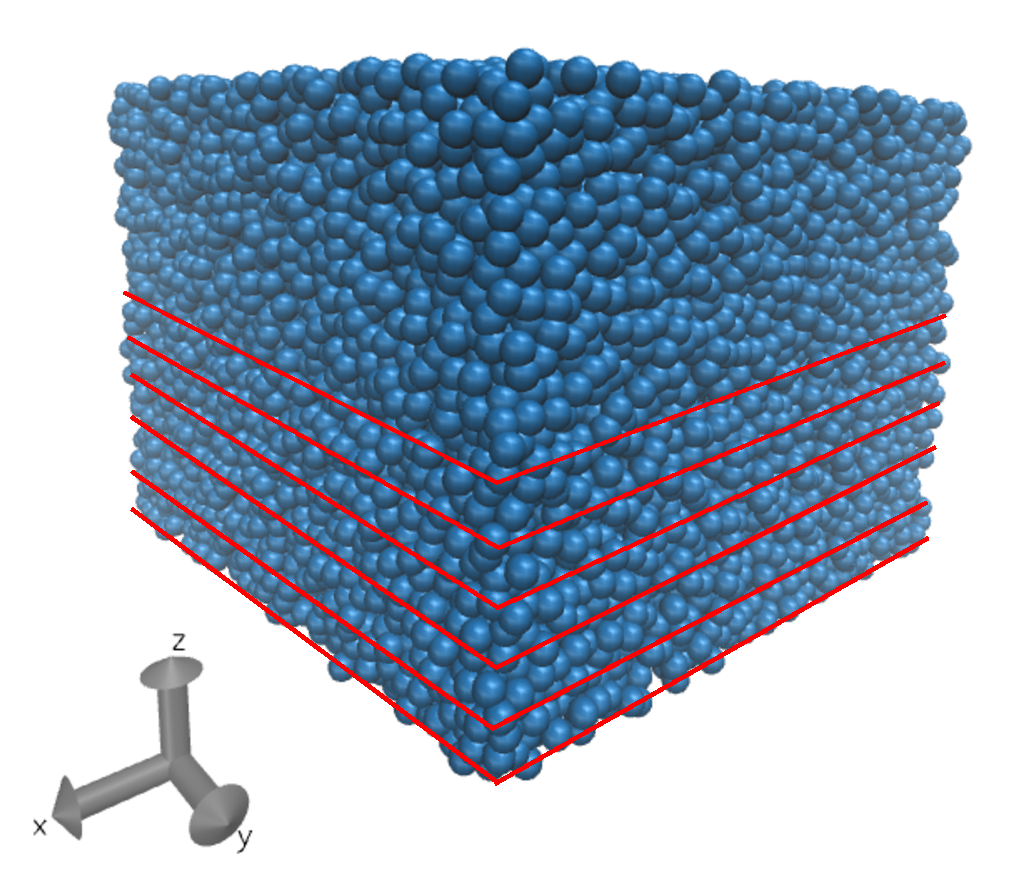
\includegraphics[scale=0.3]{system_nodes_periodic}
    \caption[Periodic box]{\Note{Pedir a Arturo esta figura}A visual representation of the MD simulation with a sketch of the binning used. In yellow are depicted the nodal planes used.}
    \label{fig:PBCBox}
\end{figure}
As we explained in Sec. \ref{Sec:DiscreteBasis}, nodes are  points  in  the $z$  axis,  while bins  are
segments in this axis.  In 3D, nodes are planes, while bins are slabs.
From  a microscopic point of  view, mass,
momentum, and force  densities are defined at the  nodes, while stress
is  defined  at  the  bins.   Each   bin  is  a  layer  of  dimensions
$L_x,L_y,\Delta z$. 


As CG variables we choose  the set of discrete hydrodynamic
variables,  which are  the  mass density  $\hat{\rho}_\mu(z)$ and  the
momentum  density $\hat{\bf  g}_\mu(z)$  defined at  the nodal  planes
$\mu$   \Note{Realmente la única variable relevante es el momento.}
\begin{align}
  \hat{\rho}_\mu(z)&= \sum_i^Nm_i\delta_\mu({\bf r}_i),&
% \nonumber\\
% \hat{e}_\mu(z)&= \sum_i^Ne_i\delta_\mu({\bf r}_i)
\hat{\bf g}_\mu(z)&= \sum_i^N{\bf p}_i\delta_\mu({\bf r}_i)
\label{rhogmumicPBC}
\end{align}
where ${\bf r}_i,{\bf p}_i$ are the position and momentum of particle $i$, and the discrete Dirac $\delta$ was introduced in (\ref{delta})
%\begin{align}
%\delta_\mu({\bf r})&=  \frac{1}{{\cal V}_\mu}\Phi_\mu({\bf r})
%\label{delta}
%\end{align}
%with the volume defined as
%\begin{align}
%  {\cal V}_\mu&=\int d{\bf r}\Phi_\mu({\bf r}),
%\end{align}
%and $\Phi_\mu({\bf r})$  is the finite element basis  function, a tent
%function centered  at the nodal plane  $\mu$ and that depends  only on
%the $z$ component  of ${\bf r}$.  The mass density  at a node receives
%information about the  mass of fluid molecule $i$ that  depends on the
%distance of this molecule to the  nodal plane $\mu$, and similarly for
%the  momentum.   
The  microscopic  variables  (\ref{rhogmumicPBC})  give,
essentially, the number  of particles and momentum per  unit volume of
the particles that happen to be ``around'' the nodal plane $\mu$.  The rationale for using this definition has been discussed in Chapter \ref{Chap:Planar}.


Note that the discrete Dirac $\delta$ function depends on the finite  element basis  function $\Phi_\mu({\bf  r})$, introduced in equation (\ref{basisFunction}), which form a
partition of unity (\ref{partition})
%\begin{align}
%  \sum_\mu\Phi_{\mu=1}^{N_{\rm bin}}({\bf r})=1
%\label{PartUnit}
%\end{align}
The  partition  of unity  implies  that  if  we compute  the  discrete
integral  (i.e. sum  over bins  times the  volume of  the bin)  of the
discrete hydrodynamic variables we obtain
\begin{align}
  \sum_\mu{\cal V}_\mu\hat{\rho}_\mu(z)&  &&= mN
\nonumber\\
  \sum_\mu{\cal V}_\mu\hat{\bf g}_\mu(z)&=\sum_i^N{\bf p}_i&&= \hat{\bf P}_T(z)
\label{DiscCons}
\end{align}
where we  have introduced the total  mass $mN$ and the  total momentum
$\hat{\bf  P}_T(z)$ of  the  system.  These  are  quantities that  are
conserved under  the Hamiltonian  evolution of the  microscopic state.


We  will only  consider the correlations  of the
component  $\hat{{\bf g}}^x_\mu$ of  the  momentum density  parallel to  the
bins. These variables are collected into the $N_{\rm bin}$-dimensional
vector           $\hat{g}(z)=\{\hat{{\bf g}}^x_1(z),\cdots,\hat{{\bf g}}^x_{N_{\rm
    bin}}(z)\}$.  We  have checked  through MD  simulations that  the coupling
between  this  component  and   the  rest  of  hydrodynamic  variables
(density,  other momentum  components) is  negligible.  Therefore,  we
expect  that a  theory  of  just the  transverse  momentum  is a  good
candidate for  a Markovian theory.  
%Sound perpendicular to  walls that
%requires both the mass density  and the perpendicular component of the
%discrete momentum will be considered elsewhere.

%\subsection{The dynamics}
%\label{Sec:Trans}
%The correlation matrix of the  CG variables $\hat{A}$, assumed to have zero
%equilibrium average, is 
%\begin{align}
%  C(t)&=\llangle \hat{A}(t)\hat{A}^T\rrangle
%\end{align}
%where the $\llangle\cdots\rrangle$ denotes the equilibrium average and
%$T$ is for transpose. 
%
%Mori theory for correlations presented in Sec. (\ref{Sec:Mori}) allows us to obtain the evolution of the matrix of correlations $C(t)$ as
%\begin{align}
%    \frac{d}{dt}C(t) = -(L+M^*)\cdot C^{-1}(0)\cdot C(t),
%\end{align}
%where we have use the equations (\ref{AproxC}), (\ref{Lambda}) and the normalized correlation matrix defined as
%\begin{align}
%  c(t)=C^{-1}(0)\esc C(t)
%\end{align}
%Note that the reversible matrix $L$ vanishes because it involves an equilibrium average of a function that is even in the momentum variables. Therefore
%\begin{align}
%    \frac{d}{dt}C(t) = -k_BTM^*\cdot c(t)
%    \label{AproxCg}
%\end{align}
%where, in order to make contact  with known results, we have redefined
%the transport  matrix $M^*$  by introducing  a prefactor  $k_BT$ where
%$k_B$ is Boltzman's constant and $T$ the equilibrium temperature. 
%%As a final
%%remark, note that the Markovian equation (\ref{AproxCg}) cannot hold at
%%$t=0$, because in that case we get $0=-k_BTM^*$, which is non-sense. Clearly,
%%such a Markovian equation can only hold beyond certain time $\tau$, related
%%to the neglected memory.

\subsection{The Green-Kubo running integral $M(t)$}
Mori theory for correlations presented in Sec. \ref{Sec:Mori} allows one to obtain the evolution of the matrix of correlations $C(t)$ as
\begin{align}
    %\frac{d}{dt}C(t) = -(L+M^*)\cdot C^{-1}(0)\cdot C(t),
    \frac{d}{dt}C(t) = -(L+M^*)\cdot c(t),
\end{align}
where we have use equations (\ref{AproxC}),  (\ref{Lambda}) and the normalized correlation matrix defined as in (\ref{cnorm}).
%\begin{align}
%  c(t)=C^{-1}(0)\esc C(t)
%\end{align}
Note that the reversible matrix $L$ vanishes because it involves an equilibrium average of a function that is even in the momentum variables. Therefore
\begin{align}
    \frac{d}{dt}C(t) = -k_BTM^*\cdot c(t),
    \label{AproxCg}
\end{align}
where, in order to make contact  with known results, we have redefined
the transport  matrix $M^*$  by introducing  a prefactor  $k_BT$ where
$k_B$ is Boltzman's constant and $T$ the equilibrium temperature. 

The friction matrix $M^*$ in (\ref{GKCorrected}) is
related to the standard Green-Kubo running integral
\begin{align}
M(t)&=\frac{1}{k_BT}\int_0^{t}dt' \llangle i{\cal L}\hat{g}(t')i{\cal L}\hat{g}^T\rrangle
\label{Mmunu}
\end{align}
that  involves the  time
derivative of the  momentum density which, as shown  in equation (\ref{equationivalence}), is
given by
\begin{align}
  i{\cal L}  \hat{g}_{\mu}(z)&=-\frac{\hat{\sigma}^{xz}_{\mu}-\hat{\sigma}^{xz}_{\mu-1}}{\Delta z}
\label{iLAcurrentx}
\end{align}
This  is a  discrete expression  of the  momentum balance  equation in
which the time rate of change of the momentum of the node $\mu$ is due
to   the   finite   difference   gradient   of   the   stress   tensor
$\hat{\sigma}^{xz}_{\mu}$  of  the  neighbour bins.   The 
microscopic   stress   tensor   of  bin $\mu$ is 

\begin{align}
 \hat{ \boldsymbol{\sigma}}_{\mu}
% &=\hat{\bf K}_\mu+\hat{\boldsymbol{\Pi}}_{\mu}
% \nonumber\\
&=
\frac{1}{{\cal V}_\mu} \left[\sum_i{\bf p}_i{\bf v}_i\chi_\mu({\bf r}_i)
+\frac{1}{2}\sum^{N}_{ij}{\bf r}_{ij}\hat{\bf F}_{ij}z_\mu(i,j)\right],
\label{sbin}
\end{align}
where $\chi_\mu({\bf r})$ is the  characteristic function of bin $\mu$
and $z_{\mu}(i,j)$, introduced in equation (\ref{geoFactor}), is the fraction of the distance between atoms $i,j$
that happens to be within bin $\mu$.

We may write equation (\ref{iLAcurrentx}) in matrix form as
\begin{align}
  i{\cal L}\hat{g}&= -B\esc\hat{\sigma}^{xz} =F^T\esc\hat{\sigma}^{xz}
\label{iLgMat}
\end{align}
where  $\hat{\sigma}$ is  a  $N_{\rm  bin}$-dimensional column  vector
containing the  discrete stress tensor  of bin  $\mu$ and $B$  is the
backward finite difference matrix.  This matrix is $B=-F^T$, where the
matrix $ F$ is the forward finite difference operator (for PBC)
\begin{align}
 {F}=\frac{1}{\Delta z}\left(
    \begin{array}{rrrrr}
-1&1&0&\cdots&0\\
0&-1&1&\cdots&0\\
\vdots      &&\ddots&&\vdots\\
\\
0&\cdots&0&-1&1 
\\
1&\cdots&0&0&-1 \end{array}
\right)
\label{Dforward}
\end{align}
By using (\ref{iLgMat}) into the Green-Kubo integral matrix $M(t)$ in (\ref{Mmunu})
we have
\begin{align}
  M(t)=F^T\esc\eta(t)\esc F,
\label{Mtfef}
\end{align}
where  the  \textit{nonlocal  viscosity  Green-Kubo  matrix}  is  the
running  time integral  of the  correlation  of the  stress tensor  at
different bins,
\begin{align}
  \eta(t) &=\frac{1}{k_BT}\int_0^{t}dt' 
  \llangle \hat{\sigma}^{xz}(t')\hat{\sigma}^{xz}\rrangle
\label{non-loc}
\end{align}
Note that  for a homogeneous system  (as one with PBC),  the nonlocal
viscosity    matrix   is    translationally    invariant,   this    is
$\eta_{\mu\nu}=\eta(|\mu-\nu|)$.  This kind  of matrices  commute with
the forward differencing matrix
\begin{align}
  F\esc\eta(t)=\eta(t)\esc F
\label{commute}
\end{align}
By using this commutation property 
 in the Green-Kubo
integral (\ref{Mtfef}) we obtain
\begin{align}
  M(t)=-\Delta\esc \eta(t),
\label{MmunuMat}
\end{align}
where we have introduced  the discrete Laplacian matrix (for PBC) as
\begin{align}
\Delta&\equiv  B\esc F
=\frac{1}{\Delta z^2}\left(
    \begin{array}{rrrrr}
-2&1&0&\cdots&1\\
1&-2&1&\cdots&0\\
\vdots      &&\ddots&&\vdots\\
\\
1&\cdots&0&1&-2    \end{array}
\right)
\end{align}

\subsection{The  friction   matrix  $M^*$  and  the   nonlocal  shear viscosity matrix}

Note that the Green-Kubo integral (\ref{Mmunu}) can also be written
in the form
\begin{align}
    M(t)&= \frac{1}{k_BT} \int_0^t dt'\frac{d}{dt'}\llangle \hat{g}(t') i{\cal L}\hat{g}^T\rrangle
\nonumber\\
&= \frac{1}{k_BT} \llangle \hat{g}(t) i{\cal L}\hat{g}^T\rrangle
=  -\frac{1}{k_BT}\frac{d}{dt}\llangle \hat{g}(t) \hat{g}^T\rrangle=-\frac{1}{k_BT}\frac{d}{dt}C(t)
\label{E1}
\end{align}
Therefore,  equations  (\ref{MmunuMat}), (\ref{E1})  lead  to  the  following
\textit{rigorous and exact} result
\begin{align}
\frac{d}{dt}C(t)&= k_BT \Delta\esc \eta(t)
\label{etaExact}
\end{align}
that links the momentum correlation matrix with the stress correlation
matrix.  This  equation shows  that  the  Green-Kubo running  integral
(\ref{non-loc})  for  the viscosity  matrix  $\eta(t)$  cannot have  a
plateau, as it should decay according to the time derivative of $C(t)$
and,  hence, from  (\ref{AproxC})  as the  correlation matrix  $C(t)$
itself.

By analogy with  (\ref{MmunuMat}), we assume that the  friction matrix $M^*$ in
(\ref{AproxCg}) has the structure
\begin{align}
  M^*=-\Delta\esc \eta^*
  \label{M*eta*}
\end{align}
for a  certain  matrix  $\eta^*$  referred to  as  the  nonlocal  shear
viscosity  matrix.  The Markovian  dynamics  (\ref{AproxCg})
becomes
\begin{align}
\frac{d}{dt}C(t)&=  k_BT\Delta\esc \eta^*\esc c(t)
\label{AproxCg1}
\end{align}
We  would like  to  obtain  the matrix  $\eta^*$  from the  Green-Kubo
running  integral   (\ref{non-loc})  for  $\eta(t)$.    Comparison  of
(\ref{AproxCg1}) and (\ref{etaExact}) gives
\begin{align}
 \Delta\esc \eta(t) &=\Delta\esc \eta^*\esc c(t)
\label{etaExact1}
\end{align}
If   the   two   matrices    $\Delta,c(t)$   were   invertible,   then
(\ref{AproxCg1}) would  allow to obtain $\eta^*$  from the correlation
of  the  momentum  density,  while equation  (\ref{etaExact1})  would  give
$\eta^*$  from the  correlation of  the  stress. Both  routes are,  of
course, mathematically equivalent.  However, both the Laplacian matrix
$\Delta$  and  the  normalized   correlation  matrix  $c(t)$  are  not
invertible.  The reason is that the normalized ``constant'' vector
\begin{align}
  v&=\frac{1}{\sqrt{N_{{\rm bin}}}}(1,1,\cdots,1)
\end{align}
is the unique eigenvector of null eigenvalue of the Laplacian operator
with periodic boundary conditions, $\Delta  \cdot v=0$. This vector is
also  eigenvector  of  null   eigenvalue  of  the  correlation  matrix
$C(t)\esc v=0$  due to total momentum  conservation in PBC. 
%Que no tengan un autovalor nulo es condición necesaria para que una matriz sea invertible.
%These two  matrices are
%not invertible, although they are so in the subspace normal to $v$. It is 
%much easier to deal with this issue in Fourier space.
In the next section we take advantage of the periodicity and the translational invariance of the system in order to deal with that issue in Fourier space. 

\subsection{Fourier space}
\label{Sec:Fourier}
Consider the unitary matrix with elements
\begin{align}
E_{\mu\nu}=\frac{1}{\sqrt{N_{\rm bin}}}\exp\left\{i\frac{2\pi}{N_{\rm bin}}\mu\nu\right\}
\end{align} 
This matrix has the following inverse
\begin{align}
E^{-1}_{\mu\nu}=\frac{1}{\sqrt{N_{\rm bin}}}\exp\left\{-i\frac{2\pi}{N_{\rm bin}}\mu\nu\right\}
\end{align} 
The indices  are assumed  to run  in the  range $\mu=0,1,\cdots,N_{\rm
  bin}-1$.  
We define the Fourier transform $\tilde{A}$ of a matrix $A$ as
\begin{align}
    \tilde{A}&=E^{-1}\esc A\esc{E}
 \end{align}
with the inverse relation 
 \begin{align}
     A&=E\esc  \tilde{A}\esc{E}^{-1}
\label{FT}
\end{align}
The discrete Laplace operator diagonalizes in Fourier space, that is,
\begin{align}
  E^{-1}  \esc {\Delta} \esc E= \tilde{\Delta},
\label{EDE}
\end{align}
where $\tilde{\Delta}$ is a diagonal matrix whose diagonal  elements are
\begin{align}
\tilde{\Delta}_{\mu\mu}&=-\frac{2}{\Delta z^2}
\left(1-\cos\left( \frac{2\pi \mu}{N_{\rm bin}}\right)\right)\le0  
\label{Dmumu}
\end{align}
This is the  spectrum of the discrete Laplace  operator $\Delta$. 


The matrix $E$ diagonalizes any traslation invariant and periodic
matrix    $A_{\mu\nu}$    satisfying    $A_{\mu\nu}=a(|\mu-\nu|)$    and
$a(\mu)=a(N_{\rm bin}-1-\mu)$ as it is easily seen
\begin{align}
\left[  E^{-1}\esc A\esc E\right]_{\mu\nu}
%\nonumber\\
&=
\frac{1}{N_{\rm bin}}\sum_{\mu'=0}^{N_{\rm bin}-1}\sum_{\nu'=0}^{N_{\rm bin}-1} e^{-i\frac{2\pi}{N_{\rm bin}}\mu\mu'}a(|\mu'-\nu'|)
e^{i\frac{2\pi}{N_{\rm bin}}\nu'\nu}
 \nonumber\\
&=\frac{1}{N_{\rm bin}}\delta_{\mu\nu}\underbrace{\sum_{\sigma=0}^{N_{\rm bin}-1}a(\sigma)e^{i\frac{2\pi}{N_{\rm bin}}\sigma\nu}}_{\tilde{a}(\nu)}
\end{align}

Because  the  matrix  $C(t)$  is periodic  traslation  invariant,  the
Fourier     transform     is     a    diagonal     periodic     matrix
$\tilde{C}_{\mu\nu}(t)=\delta_{\mu\nu}\tilde{C}_{\mu\mu}(t)$.
The two equations (\ref{AproxCg1}),(\ref{etaExact1}) become in Fourier space
\begin{align}
  \frac{d}{dt}\tilde{C}(t)&=  k_BT\tilde{\Delta}\esc \tilde{\eta}^*\esc \tilde{c}(t)
\nonumber\\
 \tilde{\Delta}\esc \tilde{\eta}(t) &=\tilde{\Delta}\esc \tilde{\eta}^*\esc \tilde{c}(t)
\label{Fou1}
\end{align}
All matrices  appearing in  these equations are  diagonal.  Therefore,
except  for $\mu=0$,  where $\tilde{c}_{00}=0$  due to  total momentum
conservation,  we  may  infer  the  diagonal  elements  of  the  shear
viscosity matrix in Fourier space  $\tilde{\eta}^*$ from either any of
these two equations
\begin{align}
  \tilde{\eta}^*_{\mu\mu}&= \frac{1}{ k_BT\tilde{\Delta}_{\mu\mu}  \tilde{c}_{\mu\mu}(t)}\frac{d}{dt}\tilde{C}_{\mu\nu}(t)
\nonumber\\
\tilde{\eta}_{\mu\mu}^*&=\frac{\tilde{\eta}_{\mu\mu}(t) }{\tilde{c}_{\mu\mu}(t)}
\label{FouFin}
\end{align}
These two expressions are mathematically  equivalent but they allow to
obtain   the    nonlocal   shear    viscosity   in    Fourier   space
$\tilde{\eta}_{\mu\mu}^*$ either  from the correlation of  momemtum or
from the  correlation of stress.   The existence  of a plateau  in the
time-dependent  functions of  the  right hand  side in  (\ref{FouFin})
constitute both, a validation of  the Markovian assumption, as well as
a way to compute the nonlocal shear viscosity.

If we wish  to recover the nonlocal shear viscosity  in real space we
need   to  know   all   their  eigenvalues.    However,  the   element
$\tilde{\eta}_{00}$  cannot be  computed  from (\ref{FouFin})  because
$\tilde{c}_{00}=0$.  Note that this value  can be obtained directly by
recognizing that
\begin{align}
    \tilde{\eta}_{00}(t)&=E_{0\mu}^{-1}\cdot\eta_{\mu\nu}(t)\cdot E_{\nu 0}=\frac{1}{N_{\rm bin}}
\sum_{\mu\nu}\eta_{\mu\nu}(t)
\label{eta00}
\end{align}
From
(\ref{sbin}) and the fact that $\chi_\mu({\bf r}),z_{\mu}(i,j)$ form a partition of unity, we have
that the total stress is the arithmetic average of the stress in each bin is given by
\begin{align}
\hat{\sigma}_T^{xz}=\frac{1}{N_{\rm bin}}\sum_\mu\hat{\sigma}_\mu^{xz}
\label{TotStress2}
\end{align}
where the  total stress $\hat\sigma_T^{xz}$ is defined  in the usual way
\begin{align}
\hat{\sigma}_T^{xz}&=\frac{1}{V_T}\left[\sum_{i}{\bf p}^1_i{\bf v}^3_i
+\frac{1}{2}\sum_{ij}{\bf r}^1_{ij}\hat{\bf F}^3_{ij}\right]
\label{TotStress}
\end{align}
and $V_T$ is the total volume of the system. 

By using (\ref{non-loc}) in (\ref{eta00}) we obtain
\begin{align}
    \tilde{\eta}_{00}(t)&=\frac{1}{N_{\rm bin}}\frac{1}{k_BT}\int_0^tdt'\llangle \sum_{\mu}\hat{\sigma}^{xz}_{\mu}(t')\sum_{\nu}\hat{\sigma}^{xz}_{\nu}\rrangle
\end{align}
Using the equation (\ref{TotStress2})
\begin{align}
    \tilde{\eta}_{00}(t)&=\frac{N_{\rm bin}}{k_BT}\int_0^tdt'\llangle \hat{\sigma}^{xz}_T(t')\hat{\sigma}^{xz}_T\rrangle
\end{align}
Introducing the \textit{local}  shear viscosity given by the standard Green-Kubo
integral
\begin{align}
  \eta_0(t) &\equiv \frac{V_T}{k_BT}\int_0^t dt'\llangle \hat{\sigma}_T^{xz}(t')\hat{\sigma}_T^{xz}
\rrangle
\label{etat}
\end{align}
we finally reach 
\begin{align}
    \tilde{\eta}_{00}(t)=\frac{N_{\rm bin}}{V_T}\eta_0(t)
\end{align}
Therefore, the eigenvalue $\tilde{\eta}_{00}(t)$ can be computed independently from
the local shear viscosity.

\subsection{The nonlocal kinematic viscosity matrix $\nu^*$}
As we will see, the notion of locality in space
is best addressed with the kinematic  viscosity, which is the nonlocal shear visocisity matrix $\eta^*$ divided by some ``mass density''. In  a discrete setting, the connection between
the  discrete momentum  and  the discrete  velocity  is slightly  more
involved than  in the continuum  for which  one has the  simple result
${\bf g}({\bf  r})=\rho({\bf r}){\bf  v}({\bf r})$.  In  the discrete,
the proportionality  between velocity and  momentum is through  a mass
density.  Let us see the details.

As  shown  in Appendix  \ref{Ap:Cov},  the  covariance $C(0)$  of  the
discrete momentum density in PBC is given by
\begin{align}
C_{\mu\nu}(0)&= \frac{k_BT}{{\cal V}_\mu} \rho_{\mu\nu},
\label{gg}
\end{align}
where we have introduced the mass density matrix $\rho_{\mu\nu}$ as
\begin{align}
  \rho_{\mu\nu}&\equiv  m{\cal V}_\mu n \left[ M^\delta_{\mu\nu}-
\frac{1}{n N}  \llangle \hat{n}_\mu\hat{n}_\nu\rrangle\right],
\label{MassMat}
\end{align}
where  $\hat{n}_\mu=\hat{\rho}_\mu/m$ is  the number  density  of node $\mu$ and $n=N/V$  is the  average
number density.  The
matrix $M^\delta_{\mu\nu}$ is given in (\ref{MM})
%\begin{align}
%  M^\delta_{\mu\nu}&=\int d{\bf r}\delta_\mu({\bf r})\delta_\nu({\bf r}) 
%\end{align}
For a system  with regular bins with constant volume  ${\cal V}$ each,
this matrix takes the form
\begin{align}
{M}^\delta&=\frac{1}{6{\cal V}}
\left(\begin{array}{cccccc}
4&1&0&\cdots &0&1\\
1&4&1&\cdots &0&0\\
\vdots&&&\ddots&&\vdots\\
0&0&0&\cdots &4&1\\
1&0&0&\cdots&1&4
\end{array}\right)
\end{align}
The last  term in (\ref{MassMat}) scales  as the inverse of  the total
number  $N$ of  particles and  it is  negligible in  the thermodynamic
limit.  However, we  should keep it as it  has observable consequences
in  our simulations.   In fact,  this  term is  responsible for  total
momentum conservation (\ref{DiscCons}), that is,
\begin{align}
  \sum_\mu{\cal V}_\mu\llangle \hat{g}_\mu\hat{g}_\nu\rrangle &=0
\end{align}
as   it   should,   because    the   total   momentum   $\sum_\mu{\cal
  V}_\mu\hat{g}_\mu$ vanishes  in the  center of mass  reference frame
that we take.

By using the explicit form (\ref{gg}) of the covariance matrix, we may
express equation (\ref{AproxCg1}) in the form
\begin{align}
\frac{d}{dt}C(t)= \Delta\esc \nu^*\esc C(t),
\label{SDECpi}
\end{align}
where we  have introduced  the nonlocal  \textit{kinematic} viscosity
matrix through the matrix
\begin{align}
\nu^*&\equiv  \eta^*\esc{\cal V}\esc \rho^{-1},
\label{nustar}
\end{align}
where ${\cal  V}$ is a diagonal  matrix that contains in  the diagonal
the volume ${\cal  V}_\mu$ of the bins.   In Fourier space equation (\ref{nustar})
takes the diagonal form
\begin{align}
  \tilde{\nu}_\mu^*&=  \frac{{\cal V}_\mu \tilde{\eta}_\mu^*}{\tilde{\rho}_\mu}
  \label{nustartilde}
\end{align}

\subsection{The equations for the average}

We now show why we refer to the matrix $\eta^*$ as the nonlocal shear
viscosity  and  to  the  matrix $\nu^*$  as  the  nonlocal  kinematic
viscosity.   According   to  Mori  theory,  which   encompass  Onsager
regression  hypothesis, the  evolution  of the  average  value of  the
discrete momentum should evolve according to a vector equation analogous to
(\ref{SDECpi}) for the correlation matrix
\begin{align}
  \frac{d}{dt}g(t)&={\cal V}\esc \Delta\esc\eta^*\esc v(t),
%   \frac{d}{dt}g(t)&=\Delta\esc
% \eta^*\esc k_BTC^{-1}(0)\esc g(t)
\label{dgDnug}
\end{align}
where we have defined the discrete velocity field $v=({\bf v}_1^{x},\cdots,{\bf v}^{x}_{N_{bin}})$ according to

\begin{align}
  {\bf v}^{x}_\mu&\equiv\sum_\nu \rho_{\mu\nu}^{-1}{\bf g}^{x}_\nu
\label{vel}
\end{align}

The matrix  $\rho_{\mu\nu}$ defined in (\ref{MassMat})  has dimensions
of a mass density and it  is fairly diagonal.  Its inverse $\rho^{-1}$
is concentrated on the diagonal (in fact, it decays exponentially fast
as we move out from the diagonal).  Because of this, we may interpret
$v_\mu$ defined in (\ref{vel}) as a velocity that contains information
about   the   discretization   method   used.    The components of
equation (\ref{dgDnug}) are
\begin{align}
  \frac{d}{dt}{\bf g}^x_\mu(t)&=
-\sum_\nu{\cal V}_\nu 
\frac{\left[
\eta^*_{\mu\nu}-\eta^*_{\mu-1\nu}-\eta^*_{\mu\nu-1}+\eta^*_{\mu-1\nu-1}\right]}{\Delta z^2}{\bf v}_\nu^{x}(t)
% \nonumber\\
% &+\hat{F}^+_\mu(t)
\end{align}
This equation for the non-equilibrium  average is identical to the one
obtained in Chapter \ref{Chap:Planar} with the Kawasaki-Gunton projector.

By a suitably relabeling  of indices and 
by using the translation invariance of the viscosity matrix we have
\begin{align}
  \frac{d}{dt}{\bf g}^x_\mu(t)&=\sum_\nu{\cal V}_\nu \eta^*_{\mu\nu}
\frac{\left[{\bf v}_{\nu+1}^{x}-2{\bf v}_{\nu}^{x}+{\bf v}_{\nu-1}^{x}\right]}{\Delta z^2}
% +\hat{F}^+_\mu(t)
% &=
% -\sum_\nu{\cal V}_\nu 
% \frac{\left[
% \eta_{\mu\nu}-\eta_{\mu-1\nu}\right]}{\Delta z}\frac{\left[\hat{v}_{\nu+1}^{x}-\hat{v}_{\nu}^{x}\right]}{\Delta z}+\hat{F}^+_\mu
\label{SDELap0} 
\end{align}

% where we have used a relabeling of indices in the sums. 
% This equation looks like a discretization of the continuum equation
% \begin{align}
%   \frac{d}{dt} g^{x}(z)&=-\partial_{z}\int dz'{\eta}(z-z')\partial_{z'} {\bf v}^{x}(z')+F_z^+
% \end{align}
% and this justifies  using the name nonlocal viscosity  for the matrix
% (\ref{non-loc})   and   the  definition   of   the   velocity  as   in
% (\ref{velocity}).
% An alternative form with further relabeling of indices is given by
% \begin{align}
%   \frac{d}{dt}\hat{g}_\mu&=
% \end{align}
equation (\ref{SDELap0}) looks    like    a   discretization    of    the    following
integro-differential  equation
\begin{align}
  \frac{d}{dt} {\bf g}^{x}(z)&=\int dz'{\eta}^*(z-z')\partial^2_{z'} {\bf v}^{x}(z')
\label{congx}
\end{align}
This is  a nonlocal generalization  of the diffusion equation  of the
continuum transverse  momentum
\begin{align}
  \partial_t {\bf g}^{x}(z)&=\nu^*_0\partial^2_{z}{\bf g}^{x}(z')
\label{congx3}
\end{align}
Equation   (\ref{congx3})   is  obtained  from  (\ref{congx})   by  setting
$\eta^*(z-z')=\eta^*_0\delta(z-z')$,   where   the   local   kinematic
viscosity is  $\nu^*_0=\eta^*_0/\rho$.  Therefore, it is  justified to
refer to the matrix $\eta^*_{\mu\nu}$ introduced in (\ref{non-loc}) as
the  nonlocal shear  viscosity matrix  and to  ${\bf v}_\mu$ introduced  in
(\ref{vel}) as the velocity.

% Note  that by  a  simple  relabelling of  indices  we  may also  write
% (\ref{SDELap0}) in the form
% \begin{align}
%   \frac{d}{dt}\hat{g}_\mu(t)&=
% \sum_\nu{\cal V}_\nu \frac{\left[\eta_{\mu+1\nu}-2\eta_{\mu\nu}+\eta_{\mu-1\nu}\right]}{\Delta z^2}
% \hat{v}_{\nu}^{x}+\hat{F}^+_\mu(t)
% \label{SDELap}
% \end{align}
% which corresponds to a continuum equation of the form
% \begin{align}
%   \frac{d}{dt} g^{x}(z)&=\partial^2_{z}\int dz'{\eta}(z-z') {\bf v}^{x}(z')+F_z^+
% \label{congx2}
% \end{align}
% This is  equation (\ref{congx}) after  two integrations by parts  and using
% the translation invariance of the shear viscosity matrix.

% Now that  we have identified, through  the velocity of the  bins, that
% the  matrix $\eta_{\mu\nu}$  is a  nonlocal shear  viscosity, we  can
% return back to momentum variables.   equation (\ref{SDELap}) can be written
% as
% \begin{align}
%   \frac{d}{dt}\hat{g}_\mu(t)&=
% \sum_{\mu'\nu'}\Delta_{\mu\mu'}{\cal V}_{\mu'} \eta_{\mu'\nu'} \rho^{-1}_{\nu'\nu}\hat{g}_{\nu}(t)+F_z^+(t)
% \label{SDELap2}
% \end{align}


\subsection{The local in time prediction}
By using (\ref{EDE})  and (\ref{Dmumu}), the Fourier  transform of the
equation of motion (\ref{SDECpi}) is then
\begin{align}
  \frac{d}{dt}\tilde{C}_{\mu}(t)&=-\frac{1}{\tau_\mu}\tilde{C}_\mu(t)  
\label{SDECpiDiag}
\end{align}
where the relaxation time $\tau_\mu$ of mode $\mu$ satisfies
\begin{align}
 \frac{1}{\tau_\mu}&\equiv \frac{2}{\Delta z^2}
\left(1-\cos\left( \frac{2\pi \mu}{N_{\rm bin}}\right)\right)
\tilde{\nu}_\mu^*
\label{taumu}
\end{align}
The  solution of  equation  (\ref{SDECpiDiag})  with ``initial  condition''
$\tilde{C}_\mu(\tau)$ at time $\tau$ is the exponential function
\begin{align}
  \tilde{C}_\mu(t)&=\exp\left\{-\frac{t-\tau}{\tau_\mu}\right\}  \tilde{C}_\mu(\tau)
\label{solexp}
\end{align}
The displacement of the initial condition to the time $\tau$ is due to
the fact that  we know that the exponential behaviour  cannot start at
$t=0$  where   the  Markovian  equation  (\ref{AproxC})   (and  hence
(\ref{SDECpiDiag})), cannot strictly hold.

The correlation matrix $C(t)$ in real space is obtained from the correlation in Fourier space in (\ref{solexp}) by equation (\ref{FT}), and leads to the result
\begin{align}
  C(t)&=\exp\left\{\Delta\esc \nu^* (t-\tau) \right\}C(\tau)
\label{Cmunut}
\end{align}
where the exponential matrix takes the form
\begin{align}
\left[\exp\left\{\Delta\esc \nu^* t \right\}\right]_{\mu\nu}
&=\frac{1}{N_{\rm bin}}\sum_{\mu'}\exp\left\{i\frac{2\pi}{N_{\rm bin}}(\mu-\nu)\mu'\right\}
\exp\left\{-\frac{t}{\tau_{\mu'}}\right\}
\label{ExpMat}
\end{align}
In summary, the prediction of  the correlation matrix in Fourier space
is given  by single exponentials,  while in real  space is given  by a
linear combination of  single exponentials. As we will  see, the later
will give rise to quasi-algebraic decay of correlations in real space.



\subsection{The local in space prediction}
The   discrete   version   of  the   local   continuum   hydrodynamics
equation (\ref{congx3}) is simply
\begin{align}
  \frac{d}{dt}{\bf g}^{x}_\mu(t)=&\nu_0\Delta_{\mu\nu}{\bf g}^{x}_\nu(t)
\label{gloc}
\end{align}
By comparing  this discrete equation  in the local  approximation with
the nonlocal  discrete equation  (\ref{dgDnug}), we conclude  that the
local approximation of the nonlocal viscosity matrix $\nu$ becomes a
diagonal matrix of the form
\begin{align}
\nu_{\mu\mu'}&\simeq \nu_0 \delta_{\mu\mu'}
\end{align}
where the local kinematic viscosity is given by
\begin{align}
\nu_0&\equiv \sum_{\mu'}\nu_{\mu\mu'} \quad \quad \quad\forall \mu
\label{nu0}
\end{align}
In the  local approximation, the differential  equation (\ref{SDECpi})
for the correlation matrix becomes
\begin{align}
  \frac{d}{dt}{C}(t)=&\nu_0{\Delta}\esc { C}(t)
  \label{LocalEq}
\end{align}
The Fourier transform of the local equation (\ref{LocalEq}) is identical to
(\ref{SDECpiDiag})  but  with  a  constant  value  for  the  kinematic
viscosity in (\ref{taumu})
\begin{align}
\tilde{\nu}^*_\mu&= \nu_0
\label{numunu0}
\end{align}
for all $\mu$. Therefore, the  local hydrodynamic prediction says that
the Fourier kinetic viscosity  coefficients $\tilde{\nu}_\mu$ take the
constant value $\nu_0$ given in (\ref{nu0}).
In the local approximation, the relaxation time (\ref{taumu}) is given by 
\begin{align}
 \frac{1}{\tau^{\rm loc}_\mu}&=\frac{2}{\Delta z^2}
\left(1-\cos\left( \frac{2\pi \mu}{N_{\rm bin}}\right)\right)
\nu_0
\label{taumuloc}
\end{align}



% {\blue In terms of
% the Fourier  transform $\tilde{\Lambda}$ of the  matrix $\Lambda$, the
% local prediction is given by a diagonal matrix that has as elements
% \begin{align}
%   \tilde{\Lambda}_{\mu\mu}=\nu_0 \frac{2}{\Delta z^2}\left(1-\cos\left( \frac{2\pi \mu}{N_{\rm bin}}\right)\right)
% \label{Lambdalocal}
% \end{align}
% }

\section{Summary of the theory and strategy in the simulations}
\label{Sec:Summary-TS}
In the  previous section  we have  considered the  theoretical results
predicted from Mori's theory for  the correlation matrix $C(t)$ of the
transverse momentum.  The correlation matrix obeys the linear equation
(\ref{AproxCg}) where the corrected Green-Kubo matrix $M^*$ is related
to the plateau problematic  Green-Kubo running integral $M(t)$ through
(\ref{GKCorrected}).  By  extracting the space derivatives  from $M^*$
and  $M(t)$  we  relate  these matrices  to  the  corrected  nonlocal
viscosity  matrix  $\eta^*$ in  (\ref{M*eta*})  and  to the  nonlocal
viscosity  matrix $\eta(t)$  in  (\ref{MmunuMat}), respectively.   The
latter has the  Green-Kubo expression (\ref{non-loc}) in  terms of the
correlation of the  stress tensor. The corrected  $\eta^*$ is obtained
from $\eta(t)$ through the equations (\ref{FouFin}) in Fourier space.

In order to  discuss the local approximation in space  in the equation
for the average of the  momentum field (\ref{dgDnug}) it is convenient
to introduce the kinematic viscosity matrix (\ref{nustar}) because the
local approximation  is very simple in  Fourier space in terms  of the
kinematic viscosity matrix. The local approximation amounts to set all
the  eigenvalues of  the kinematic  matrix identical  to the  standard
kinematic viscosity of the fluid, as in (\ref{numunu0}).

In the  next section we  measure through  MD simulations the  two main
quantities of concern  in this chapter which are  the correlation matrix
of discrete momentum $C(t)$ and the correlation matrix of the discrete
stress that appears in the Green-Kubo running integral $\eta(t)$. From
these  primary   quantities,  we   obtain  their   Fourier  transforms
$\tilde{C}(t),\tilde{\eta}(t)$  which  are  diagonal matrices  due  to
translation invariance.

In  order to  test  the locality  in  time, we  check  for the  simple
exponential decay prediction (\ref{solexp}) for the eigenvalues of the
correlation matrix.  In order to  test the nonlocality in space, from
equation  (\ref{FouFin}) we will infer the nonlocal shear viscosity matrix
$\tilde{\eta}^*$ and, from the  Fourier transform of (\ref{nustar}), the
nonlocal    kinematic   viscosity    $\tilde{\nu}^*$.    The    local
approximation  in   space  will   be  good   if  we   can  approximate
$\tilde{\nu}^*$  as   in  (\ref{numunu0}).   Once  we   have  measured
$\Lambda^*$ or  equivalently $\eta^*$  or $\nu^*$  we can  compare the
prediction (\ref{Cmunut}) from Mori theory with the correlation matrix
measured in the simulation.


\section{Simulations}
\label{Sec:SimPBC}
In Sec. \ref{Sec:MoriPBC} we saw that the  two main  quantities of  concern  are the  correlation matrix  of
discrete momentum  $C(t)$ and the  correlation matrix of  the discrete
stress  that appears  in  the Green-Kubo  running integral  $\eta(t)$.
These two  matrices can be measured  from MD simulations.
%In  order to
%test the locality in time, we use the simple prediction (\ref{solexp})
%for the  eigenvalues of the correlation  matrix. In order to  test the
%nonlocality  in space,  from equation   (\ref{FouFin}) we  will infer  the
%nonlocal shear viscosity matrix  $\tilde{\eta}^*$ and from the Fourier
%transform   of  (\ref{nustar})   the  nonlocal   kinematic  viscosity
%$\tilde{\nu}^*$. The local  approximation in space will be  good if we
%can approximate  $\tilde{\nu}^*$ as in (\ref{numunu0}).   Once we have
%measured  $\Lambda^*$  or  equivalently  $\eta^*$ or  $\nu^*$  we  can
%compare  the  prediction  (\ref{Cmunut})  from Mori  theory  with  the
%correlation matrix measured in the simulation.

The objective of this section is to present the simulations we made to measure the
momentum  correlation  matrix  $C(t)$  and  the  Green-Kubo  nonlocal
viscosity $\eta(t)$.   From these primary quantities,  we obtain their
Fourier transforms  $\tilde{C}(t),\tilde{\eta}(t)$ which  are diagonal
matrices  due to  traslation invariance.  

\subsection{Simulation set up}
\label{Sec:SimSetUpPBC}
A  system  of particles  interacting  with  a Lennard-Jones  potential
truncated at  $\sigma=2.5$ has been  simulated in PBC with  the LAMMPS code \cite{Plimpton1995}.
In Fig. \ref{fig:PBCBox} a snapshot of the simulation is showed.
The box  size is $40\times40\times30$, the  number of particles
is $N=28749$, and the time step is $0.002$ in reduced units.  After an
equilibration  of  $10^5$ timesteps  with  a  Langevin thermostate  to
produce a microstate typical  from a thermodynamic point corresponding
to $T=2,\rho=0.6$  in reduced units,  the system is evolved  under NVE
microcanonical conditions for a  further $10^5$ timesteps.  After this
equilibration phase,  production runs  of $1.5\times 10^6$  time steps
are launched.  The  $z$ axis is binned  in $60$ bins on  which the $x$
component of the momentum density is recorded every 10 timesteps.  The
width of the  bin is $\Delta z=0.5\sigma$ which is  subatomic.  We will see in the next chapter that in the
presence of walls,  such a bin allows to capture some of the density layering.  A total of $60\times  60$ correlations corresponding to the
elements of  the correlation matrix  are computed in  each simulation.
In  order  to increase  statistics,  we  average  the result  of  $30$
simulations and  exploit the  translation invariance  of the  system by
further  averaging correlations  between  nodes at  a given  distance.
Although  computing  all  the  correlation matrix  elements  may  seem
unnecessary, we will  use the same methodology for  confined fluids in
the next chapter. In this later case, translation invariance is
broken and we need to consider the full correlation matrix.
%\begin{align}
%  V_{ij}(r_{ij}) = \left\lbrace
%  \begin{array}{ll}
%    4\epsilon_{ij}\left[\left(\frac{\sigma_{ij}}{r_{ij}}\right)^{12}-\left(\frac{\sigma_{ij}}{r_{ij}}\right)^6\right] & \textup{if } r_{ij}\leq r_c \\
%    0 & \textup{if } r_{ij}>r_c
%  \end{array}
%  \right.
%  \label{LJ}
%\end{align}
%where $r_{ij}$ is the distance between particles $i$ and $j$, $\epsilon_{ij}$ is the depth of the potential well, $\sigma_{ij}$ is the distance at which $V_{ij}$ is zero, and $r_c$ is the cutoff radius (taken equal to $2.5\sigma_{ij}$). The parameters $\epsilon_{ij}$ and $\sigma_{ij}$ take the value 1. 

%The box  size is $40\times40\times30$, the  number of particles with mass $m=1$
%is $N=28749$, and the time step is $0.002$ in reduced units.  After an
%equilibration  of  $10^5$ timesteps  with  a  Langevin thermostate  to
%produce a microstate typical  from a thermodynamic point corresponding
%to $T=2,\rho=0.6$ in  reduced units, the system is  evolved under NVE
%microcanonical conditions for a  further $10^5$ timesteps.  After this
%equilibration  phase,  production  runs   of  $15\cdot 10^5$  time  steps  are
%launched.   The $z$  axis is  binned  in $60$  bins on  which the  $x$
%component of the momentum density is recorded.  The
%width of the  bin is $\Delta z=0.5\sigma$ which is  subatomic.  In the
%presence of walls,  such a bin allows to resolve  the density layering.  A total of $60\times  60$ correlations corresponding to the
%elements of  the correlation matrix  are computed in  each simulation.
%The correlations are computed with the LAMMPS command {\it fix ave/correlate}. During $7.5\cdot 10^5$ time steps the $x$ component of the momentum density is recorded every $2$ time steps. These values are used to obtain the correlations with a support of $15\cdot10^4$ time steps. %LAMMPS 7500 puntos curva de correlación separados por 2*dt-> soporte de 15000 (i.e. t=30)
%After $7.5\cdot 10^5$ steps the correlations are averaged with the previous one. 
%In  order to  increase  statistics,  we 
%exploit   the   traslation   invariance   of   the
%system.  Although computing  all the  correlation matrix  elements may
%seem  unnecessary,  we will  use  the  same methodology  for  confined
%fluids. In  this later  case, traslation invariance  is broken  and we
%need to consider the full correlation matrix.

\subsection{The correlation matrix $C(t)$}

In  Fig. \ref{fig:Ct-matrix-PBC} we  plot the  correlation  matrix of  the
transverse     momentum      $C_{\mu\nu}(t)=\llangle     g_{\mu}(t)\
g_\nu\rrangle$ at  the time  $t=0$ and $t=0.6$.  This  matrix is  periodic and
traslation invariant.  Therefore, statistical errors have been further
reduced by averaging this matrix ``along diagonals''.  In addition, we
have taken advantadge of the  analytical calculation of the covariance
$\llangle g_{\mu} g_\nu\rrangle$ in the Appendix \ref{Ap:Cov} in a
manner that we describe below.

\begin{figure}[h!]
\centering
%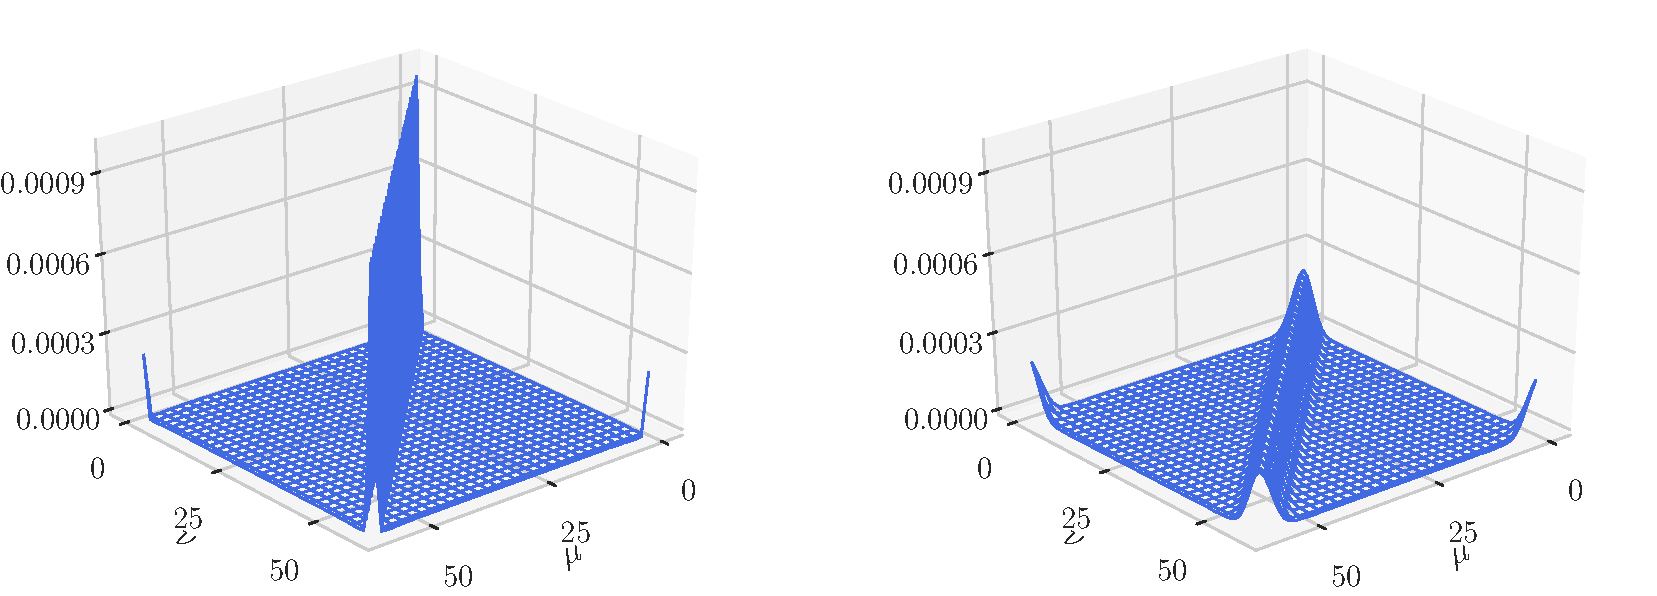
\includegraphics[scale=0.4]{Ct-matrix-PBC}
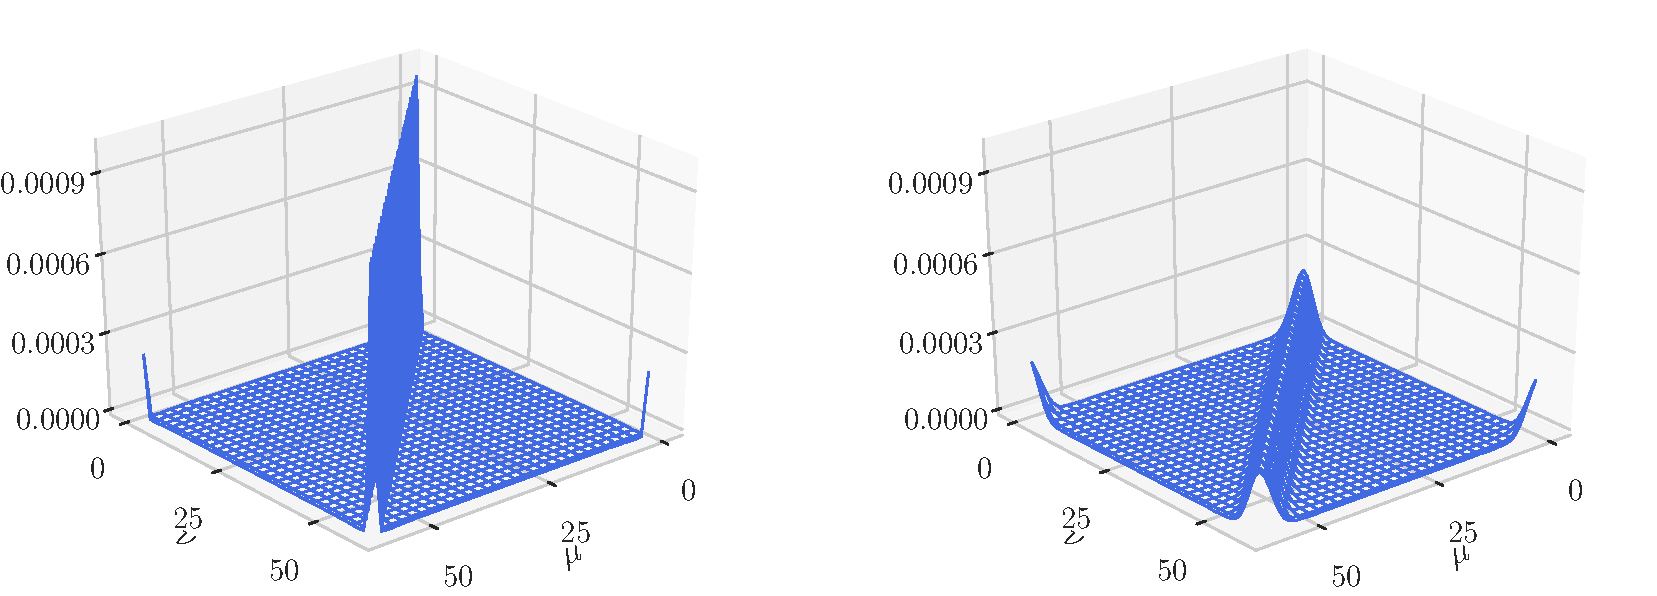
\includegraphics[width=\linewidth]{Ct-matrix-PBC}
\caption[Correlation matrix $C(t)$ at $t=0$ and $t=0.6$ for PBC system.]{The   correlation    matrix   $C_{\mu\nu}(t)=\llangle
g_{\mu}(t)  g_\nu\rrangle$ for  $t=0$ (left) and $t=0.6$ (right).}
\label{fig:Ct-matrix-PBC}
\end{figure}

In  Fig.    \ref{fig:Ct-mu30nu-PBC}  the   correlations  $\llangle
g_{\mu}(t)  g_\nu\rrangle$ for  $\mu=30$ and  different values  of
$\nu$ at $t=0$ (blue), $t=0.2$ (orange), $t=0.4$ (purple) and $t= 0.6$ (green) is shown.  This is the row 30 of the matrix plotted
in Fig. \ref{fig:Ct-matrix-PBC}.  We  observe a diffusive
behaviour over  a negative  background.  The  origin of  this negative
global  correlation for  nodes that  are far  appart is  due to  total
momentum conservation in PBC.  If a bin has  a positive momentum, the rest of
bins should  have an  overall negative  value in  order for  the total
momentum to  be zero. In order  to improve the statistical  quality of
the matrix  $C(t)$ we have  used the analytical value  (\ref{Cneg}) of
the  background,  as  provided  by the  analytic  calculation  of  the
covariance in the Appendix \ref{Ap:Cov}.\Note{¿Cómo hicimo esto?:/}

\begin{figure}[h!]
\centering
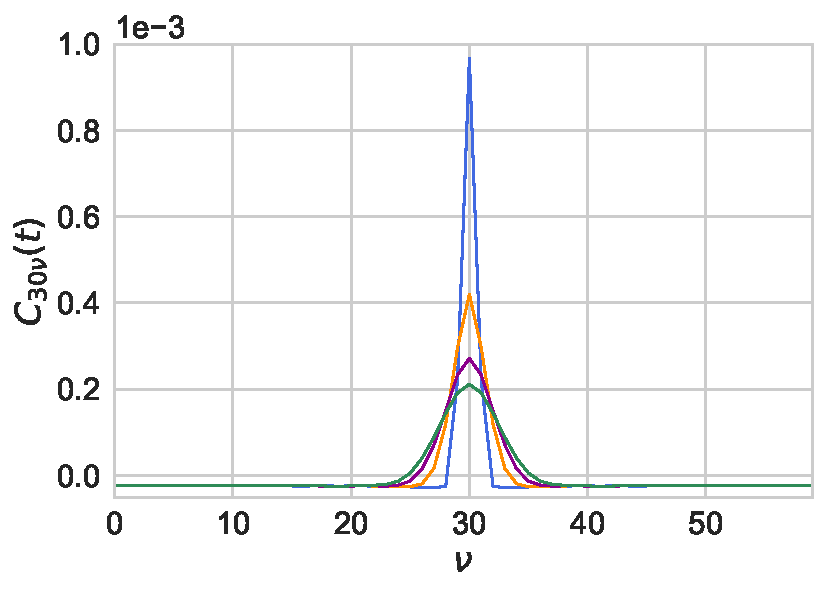
\includegraphics[scale=0.41]{Ct-mu30nu-PBC}
\caption[$C_{30\nu}(t)$ for PBC system.]{$C_{\mu\nu}(t)=\llangle  g_{\mu}(t) g_\nu\rrangle$  for $\nu=30$
 as a  function of node index  $\nu$ and for times $t=0, 0.2, 0.4, 0.6$ in descending order.}
 \label{fig:Ct-mu30nu-PBC} 
\end{figure}

The autocorrelation $\llangle  g_{\mu}(t) g_\mu\rrangle$ (which is
the same for  all $\mu$) is shown in  Fig.  \ref{fig:Autocorrelation-PBC}
as a function of time in both  linear and log scales.  Also shown is a
function $\propto  t^{-1/2}$.  The observed decay  does not correspond
to this algebraic decay.  As discussed in Appendix \ref{Ap:Cont}, only
in both,  the continuum and  thermodynamic limits, we expect  the long
time  tail   $\propto  t^{-1/2}$  behaviour  predicted   by  continuum
hydrodynamics.

\begin{figure}[h!]
\centering
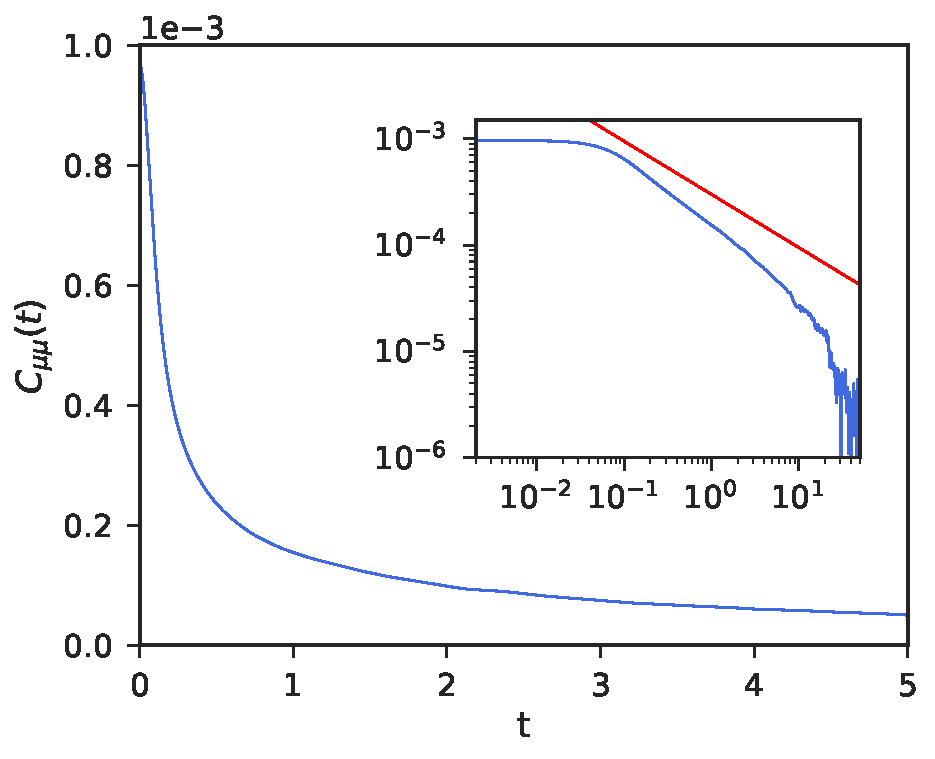
\includegraphics[scale=0.41]{Ct-mu30nu30-PBC}
\caption[Autocorrelation for PBC system.]{The autocorrelation
  $\llangle g_{\mu}(t) g_\mu\rrangle$ (for  any $\mu$)
  . The correlation  decays very
slowly, in an  apparent algebraic way as can be  seen in logscale in the inset.}
  \label{fig:Autocorrelation-PBC}
\end{figure}


\begin{figure}[h!]
  \centering
  %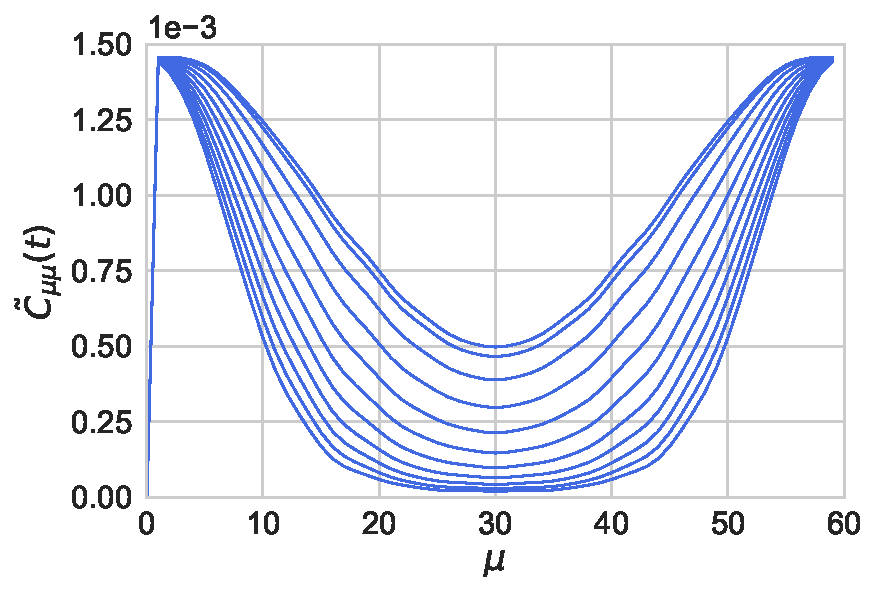
\includegraphics[scale=0.41]{CtFourier-PBC}
  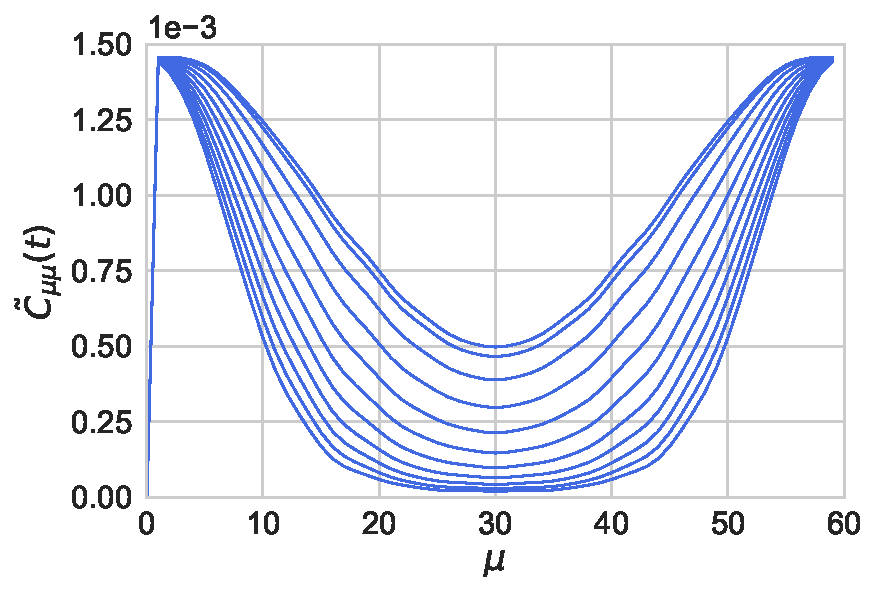
\includegraphics[scale=0.41]{CtFourier-PBC}
  \caption[Diagonal $\tilde{C}_{\mu\nu}(t)$ for PBC]{The diagonal $\tilde{C}_{\mu\mu}(t)$ of the Fourier transform
  of the correlation  matrix $C(t)$ for different values  of the time.
In      descending     order      the     plotted      times go from $t=0.10$ to $t=0.20$ in intervals of $0.02$. }
\label{fig:CtFourier-PBC}
\end{figure}

\begin{figure}[h!]
  \centering
  %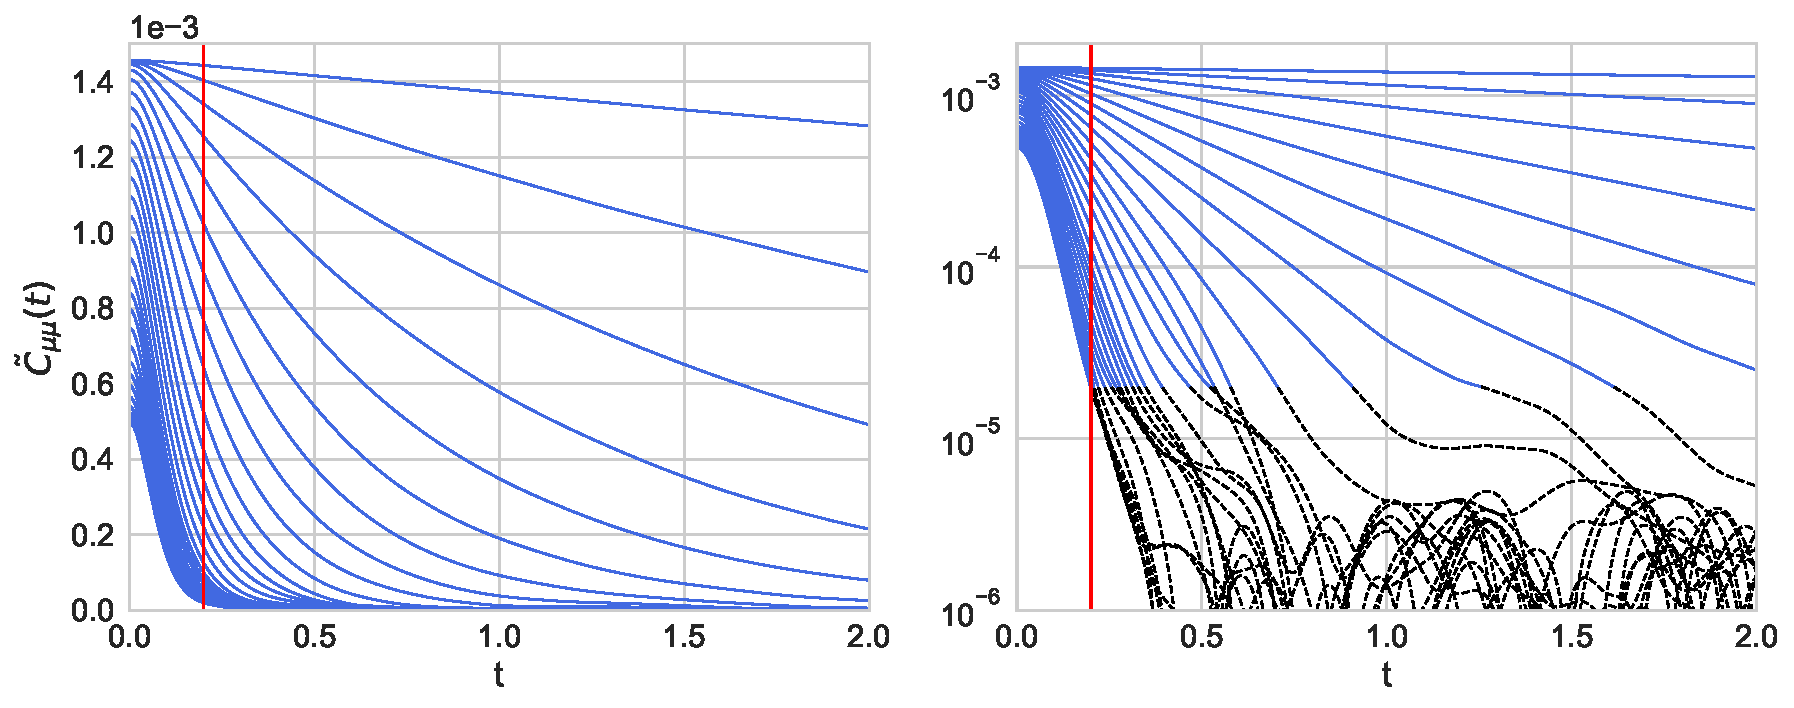
\includegraphics[scale=0.41]{CtFourier-PBC-exp}
  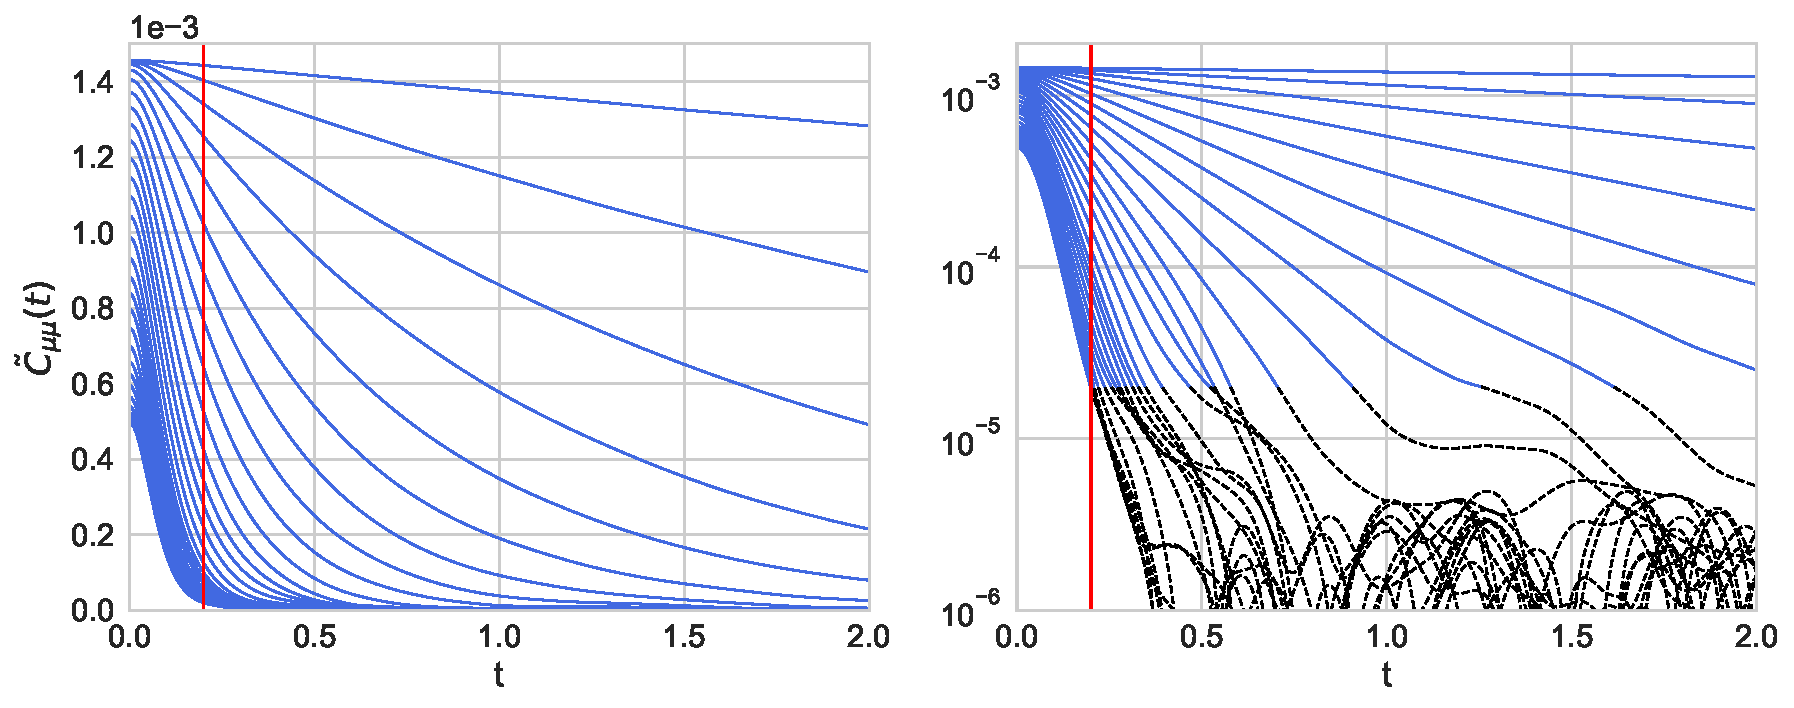
\includegraphics[width=\linewidth]{CtFourier-PBC-exp}
  \caption[Evolution of different eigenvalues $\tilde{C}_{\mu\nu}(t)$ for PBC]{
  The  evolution of  the different
  eigenvalues  $\tilde{C}_{\mu\mu}(t)$ of  the  correlation matrix  of
  momentum  as  a  function  of   time  in  a  lin-lin  plot  (left)
  and   log-lin   plot
  (right). Also  plotted are  a vertical line  at $t=\tau=0.2$  and a
  horizontal  line  at  the   value  $2\times10^{-5}$,  signaling  the
  threshold below which statistical errors give spurious results. }
\label{fig:CtFourier-PBC-exp}
\end{figure}

The Fourier transform $\tilde{C}(t)$  of the correlation matrix $C(t)$
is a diagonal matrix.  The diagonal $\tilde{C}_{\mu\mu}(t)$ is plotted
in Fig.   \ref{fig:CtFourier-PBC} as a function of the mode
$\mu$      for      different       values      of      the      time,
from $t=0.10$ to $t=0.20$ in intervals of $0.02$ in  descending   order.   Note that the  mode
$\mu=0$ gives a vanishing value  because of momentum conservation. At the largest times plotted,
the  value  of  the  diagonal  correlation  matrix  in  Fourier  space
$\tilde{C}_\mu(t)$ goes to  zero for modes with  values near $\mu=30$,
implying the  amplification of the  statistical errors in  the inverse
matrix in that  region.  In the left panel of Fig.  \ref{fig:CtFourier-PBC-exp} we
plot the  eigenvalues $\tilde{C}_{\mu\mu}(t)$  as a function  of time.
Observe  that after  a time  around  $\tau=0.2$ (red line) the  decay in  log-lin
(right  panel) is  approximately  linear,  suggesting an  exponential
decay. Also we have represented in black and dashed lines the values of the eigenvalues $\tilde{C}_{\mu\nu}$ which statistical errors give spurious results. 


\subsection{Validation of the Markov property}
\label{Sec:ValidateMarkovPBC}
When the  Markov equation (\ref{AproxC})  is valid, we have  that the
eigenvalues of  the correlation matrix decay  exponentially, according
to the prediction (\ref{SDECpiDiag}).  In order to better discriminate
the exponential behaviour we introduce the time-dependent matrix
\begin{align}
\Lambda(t)\equiv-    \frac{dC}{dt}(t)\esc C^{-1}(t)
\label{AproxCtau}
\end{align}
that according  to the Markov equation  (\ref{AproxC}), should evolve
toward a constant time  independent matrix $ \Lambda(t)\to \Lambda^*$
after   certain  time.   In  Fourier   space  all   matrices  in   equation
(\ref{AproxCtau}) are diagonal and, therefore
\begin{align}
\tilde{\Lambda}_{\mu\mu}(t)\equiv -    \frac{1}{\tilde{C}_{\mu\mu}(t)}\frac{d\tilde{C}_{\mu\mu}}{dt}(t)
\label{AproxCtau2}
\end{align}
Note that for times $t>\tau$ we have that $\tilde{\Lambda}_{\mu\mu}(t)\to \frac{1}{\tau_\mu}$
where the relaxation time is given in equation (\ref{taumu}).
\begin{figure}[h!]
  \centering
%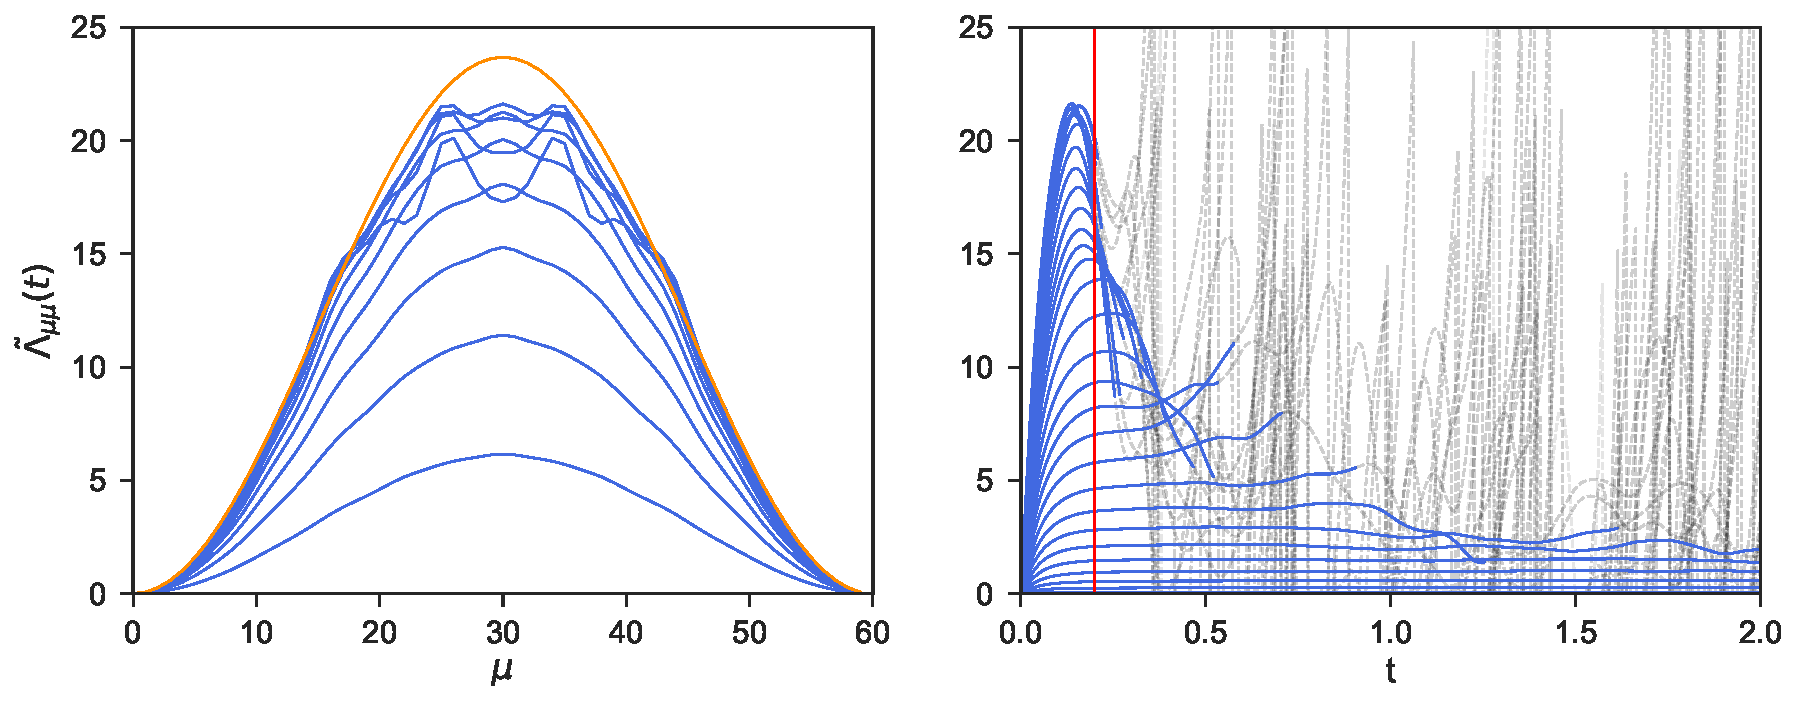
\includegraphics[scale=0.41]{LambdatFourier-PBC}
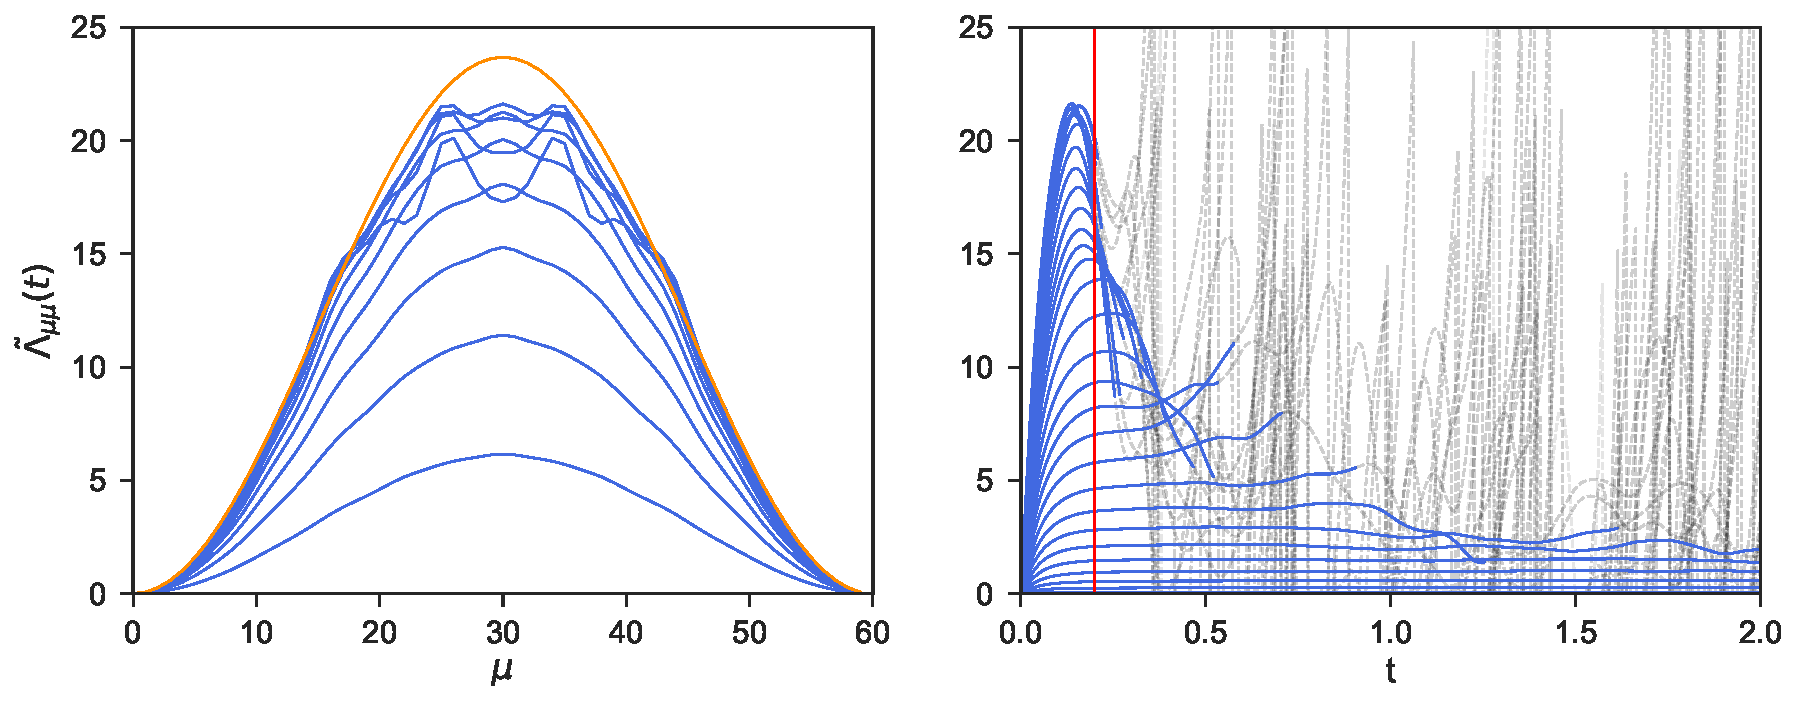
\includegraphics[width=\linewidth]{LambdatFourier-PBC}
\caption[Diagonal elements  $\tilde{\Lambda}_{\mu\mu}(t)$ of  the Fourier transform of $\Lambda(t)$]{The  diagonal elements  $\tilde{\Lambda}_{\mu\mu}(t)$ of  the
  Fourier transform of $\Lambda(t)$ defined in (\ref{AproxCtau}), as a
  function of  $\mu$ (left)  and $t$  (right).  In  the left  panel, in
  ascending  order the  plotted times  go  from $t=0$  to $t=0.20$  in
  intervals of $0.02$.  The orange line is the local approximation equation
  (\ref{Lambdaloc}) with a  value of the local  kinematic viscosity of
  $\nu_0=1.48$.   In the  right panel,  we observe  a clear  plateau,
  beyond  $\tau=0.2$ (red line) indicating  the  exponential  behaviour  of  the
  correlations in Fig. \ref{fig:CtFourier-PBC-exp}.}
\label{fig:LambdatFourier-PBC}
\end{figure}

In       Fig.         \ref{fig:LambdatFourier-PBC}       we       plot
$\tilde{\Lambda}_{\mu\mu}(t)$  as a  function of  $\mu$ for  different
times (left) and as a function of $t$ for the different values of $\mu$
(right). In the left panel,  the different curves correspond to values
of  $t$ from  $0$ to  $0.20$ in  intervals of  $0.02$.  The  structure
observed  in the  central region  is spureous  and due  to statistical
errors.   These   errors  increase  with   time.   We  also   plot  in
Fig. \ref{fig:LambdatFourier-PBC}  the theoretical prediction  of this
matrix in the local approximation  given in equation (\ref{taumuloc}) for a
fitted value  of the  local kinematic  viscosity of  $\nu_0=1.48$, which is the value of the kinematic viscosity for this system and thermodynamic point, as reported in the literature \cite{Woodcock2006}. We
observe that  the local approximation (\ref{taumuloc})  gives a fairly
reasonable approximation  for the converged  value $\tilde{\Lambda}^*$
of the  relaxation matrix in Fourier  space.  In the right  panel, we
plot $\tilde{\Lambda}_{\mu\mu}(t)$ for all $\mu$ as a function of time
$t$.  We  have disregarded the data  points beyond times in  which the
statistical  errors  lead  to  meaningless results  (those  below  the
threshold  in  the  eigenvalues  in Fig  \ref{fig:CtFourier-PBC-exp}).   We  may
appreciate a  very clear  plateau for  the modes  of low  $\mu$ (large
wavelengths) \Note{Entender bien la relación entre los modos y la longitud de onda.}.  As the wavenumber increases, for wavenumbers $\mu\ge20$
the plateau dissappears  and this is concomittant  with the appearance
of great distorsions that are due  to the lack of statistics necessary
to describe  the inverse  of the correlation matrix.  Therefore, we  cannot decide
from the plots  wether there is no plateau at  large wavenumber or, on
the contrary,  there is a  plateau but it is  obscured by the  lack of
statistics. 
Hence, we select the  time $\tau=0.2$ as
the best compromise  satisfying that $\tilde{\Lambda}_{\mu\mu}(t)$ has
attained  its  constant  value  but  does  not  suffer  from  dramatic
statistical errors.     The existence  of a  plateau
beyond  $\tau=0.2$  signals  to   the  exponential  behaviour  of  the
correlations  in  Fig.   \ref{fig:CtFourier-PBC-exp}  beyond  this  time.   We
measure  then   the  relaxation   matrix  in  Fourier   space  through
$\tilde{\Lambda}^*_{\mu\mu}=\tilde{\Lambda}_{\mu\mu}(\tau)$.      This
measured relaxation  matrix is  compared with its  local approximation
$\tilde{\Lambda}^{\rm loc}_{\mu\mu}$ which, from equation (\ref{taumuloc}),
is given by
\begin{align}
\tilde{\Lambda}^{\rm loc}_{\mu\mu}&=\frac{2}{\Delta z^2}
\left(1-\cos\left( \frac{2\pi \mu}{N_{\rm bin}}\right)\right)
\nu_0
\label{Lambdaloc}
\end{align}

\begin{figure}[h!]
  \centering
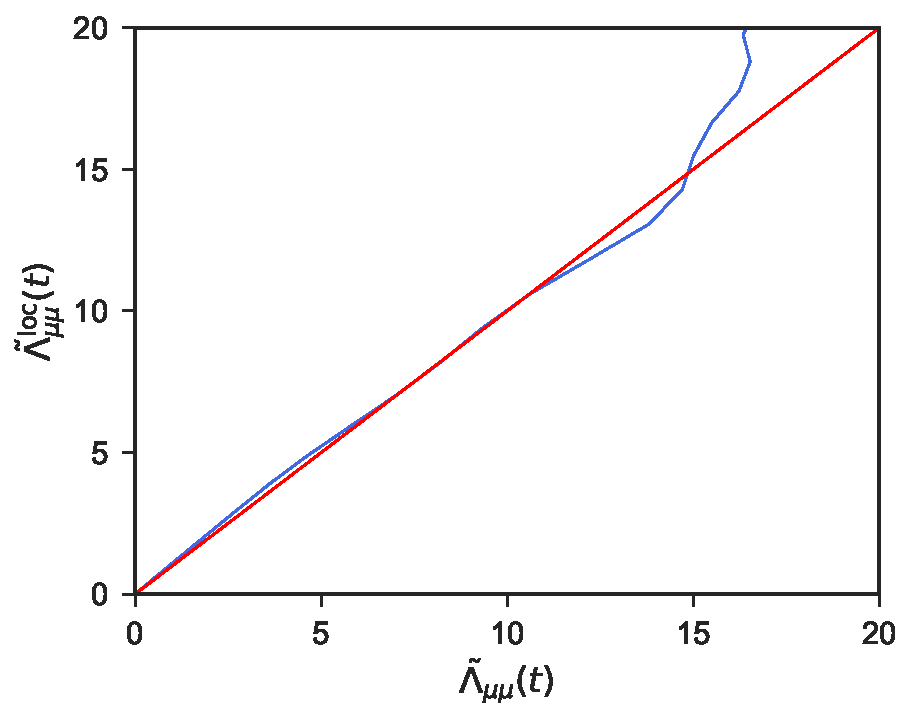
\includegraphics[scale=0.41]{CompareLambdas-PBC}
\caption[Comparison $\tilde{\Lambda}^*_{\mu\mu}$ and $\tilde{\Lambda}_{\mu\mu}(\tau)$]{Comparison $\tilde{\Lambda}^*_{\mu\mu}=\tilde{\Lambda}_{\mu\mu}(\tau)$ for $\tau=0.2$ with $\tilde{\Lambda}^{\rm loc}_{\mu\mu}$ in equation (\ref{Lambdaloc}) with $\nu_0=1.48$. The red line has slope $1$ and it is for guide the eye.}
\label{fig:CompareLambdas-PBC}
\end{figure}
In         Fig.           \ref{fig:CompareLambdas-PBC}         we         plot
$\tilde{\Lambda}^*_{\mu\mu}=\tilde{\Lambda}_{\mu\mu}(\tau)$        for
$\tau=0.2$    against    $\tilde{\Lambda}_{\mu\mu}^{\rm    loc}$    in
(\ref{Lambdaloc})   with  $\nu_0=1.48$. Observe that the linear behaviour of this plot
indicates  that,  to  a  very good  degree,  the  local  approximation
describes well the relaxation matrix $\Lambda^*$.
From the Fourier transform  of the diagonal matrix $\tilde{\Lambda}^*$
we may  obtain the relaxation  matrix $\Lambda^*$ in real space which,  by comparing
(\ref{AproxC})      with     (\ref{SDECpi})      is     given      by
$\Lambda^*=\Delta\nu^*$. From equation  (\ref{Cmunut}) we can
now  have the  prediction of  Mori theory  for the  correlation matrix
$C(t)$.  In Fig.  \ref{fig:Predictionsmumu-PBC} we compare the autocorrelation
$C_{\mu\mu}(t)$ measured in  MD with the predictions  of the nonlocal
(orange) and local  (green) theories.  The arrow is at  $t=\tau$ where the
three curves  coincide by  construction.  The  agreement of  the three
curves  is  excellent beyond  $\tau$.   This  is best  appreciated  in
logscale (right panel). The curving at long times,
reflecting the  finite size  of the simulation  box (see  Appendix \ref{Ap:Cov}) is
captured in  both theories.  The inset  in the left panel of Fig.  \ref{fig:Predictionsmumu-PBC}
shows a zoom at short times,  where one appreciates that the nonlocal
theory gives  a better  prediction than the  local prediction  but, of
course,  yields  poor results  at  very  short  times. Note  that  the
Markovian theory leads to a cusp at $t=0$ in the correlation while the
MD  results  have   a  vanishing  value  of  the   derivative  of  the
correlation.

\begin{figure}[h!]
  \centering
%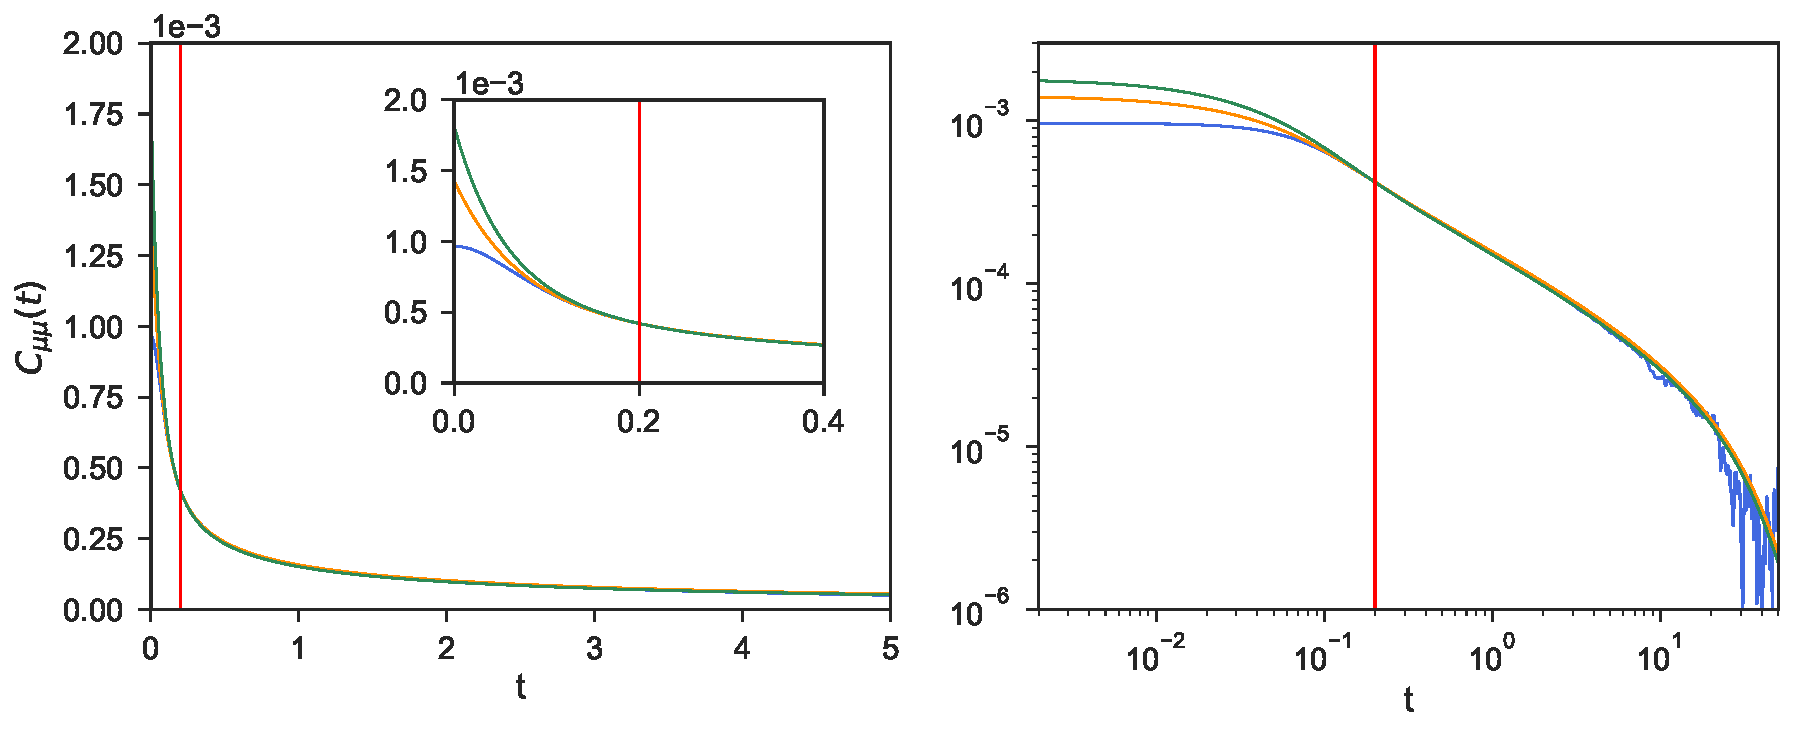
\includegraphics[scale=0.41]{Predictionsmumu-PBC}
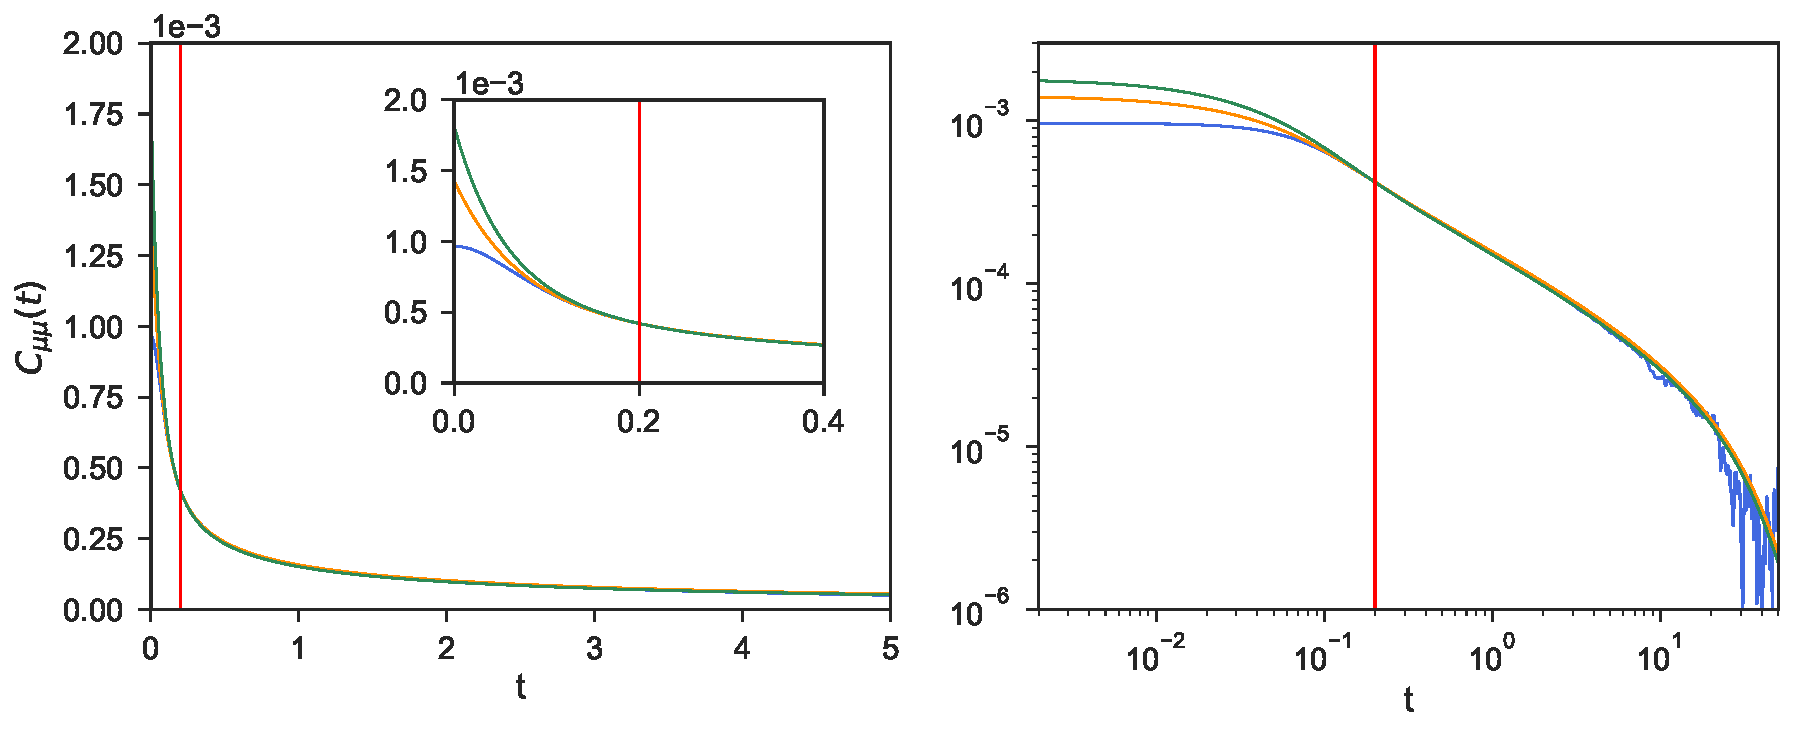
\includegraphics[width=\linewidth]{Predictionsmumu-PBC}
\caption[Comparison of autocorrelation $C_{\mu\mu}$ with the predicions for PBC system]{Comparison of autocorrelation $C_{\mu\mu}(t)$ with the predictions of the nonlocal (orange) and local (green) theries. The left panel is in linscale and the right panel in logscale. The red line is at $t=\tau$ where the three curves coincide by construction. The inset shows a zoom at short times.}
\label{fig:Predictionsmumu-PBC}
\end{figure}

In Fig. \ref{fig:Predictionsmumu+1-PBC} we compare the cross correlation $C_{\mu\mu+1}(t)$ in the same way as we did with the autocorrelation in Fig. \ref{fig:Predictionsmumu-PBC}. The agreement of the the three curves (predictions, nonlocal and local theories) is excellent beyond $\tau$, but we appreciate that for long times the local prediction is better than the nonlocal prediction. 

\begin{figure}[h!]
  \centering
%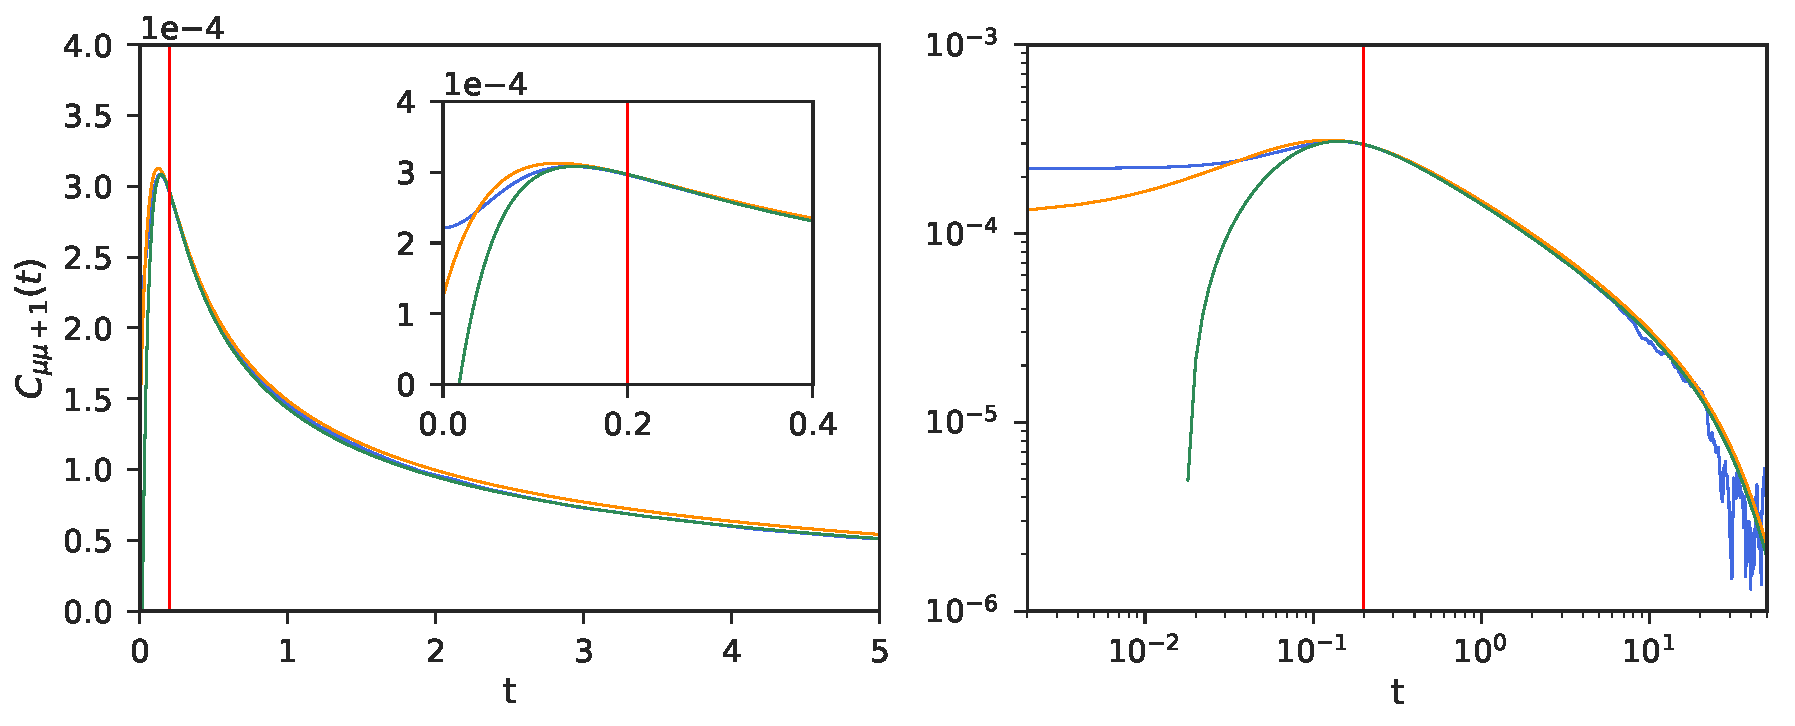
\includegraphics[scale=0.41]{Predictionsmumu+1-PBC}
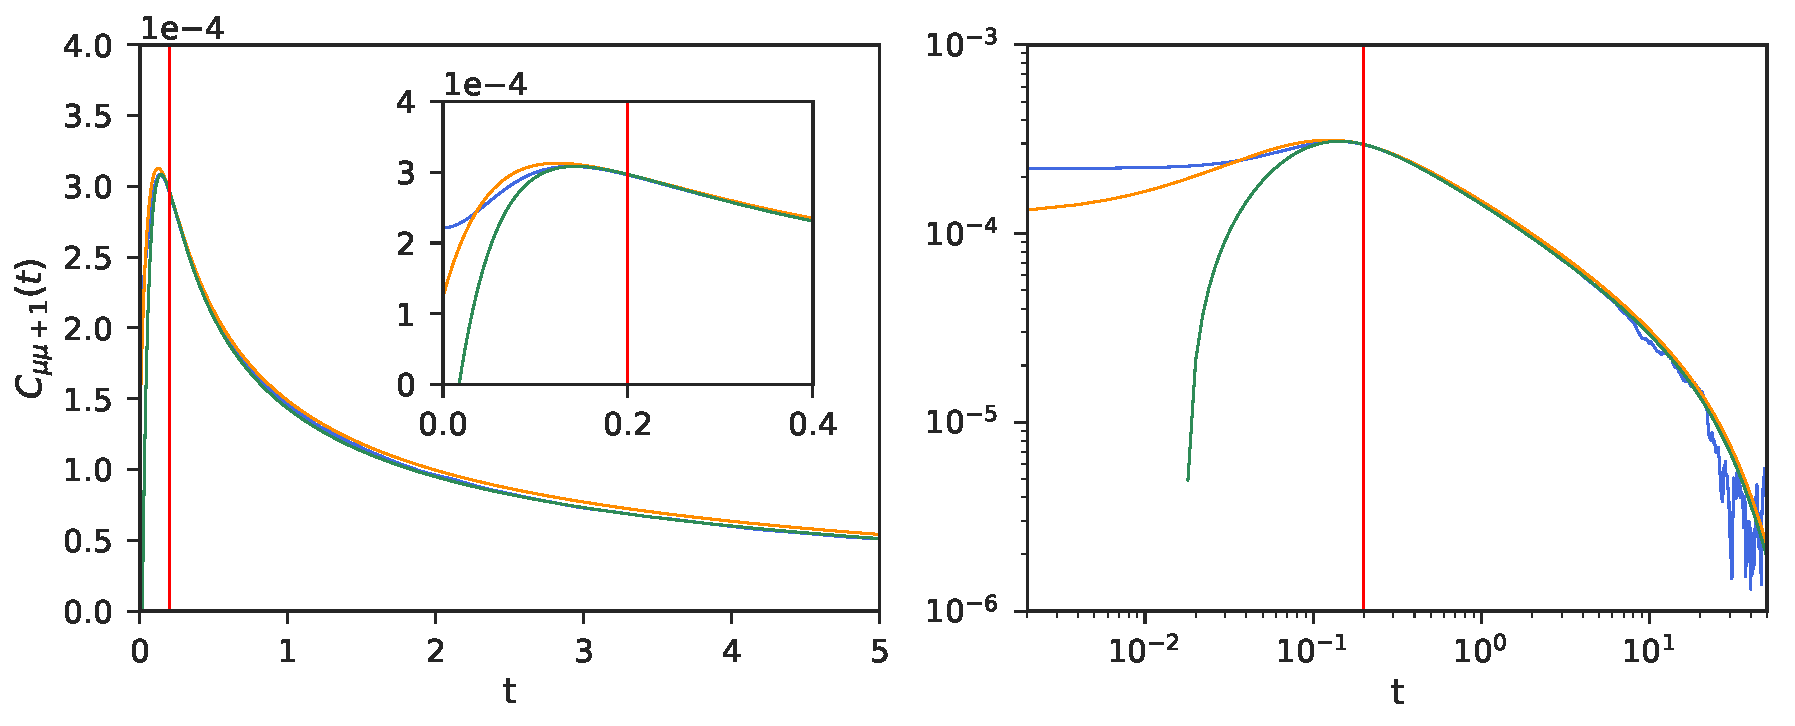
\includegraphics[width=\linewidth]{Predictionsmumu+1-PBC}
\caption[Comparison of cross correlation $C_{\mu\mu+1}$ with the predicions for PBC system]{Comparison of autocorrelation $C_{\mu\mu+1}(t)$ with the predictions of the nonlocal (orange) and local (green) theries. The left panel is in linscale and the right panel in logscale. The red line is at $t=\tau$ where the three curves coincide by construction. The inset shows a zoom at short times.}
\label{fig:Predictionsmumu+1-PBC}
\end{figure}

In summary, in the present subsection we have shown that the Markovian
approximation  is  an   excellent  one  for  the   prediction  of  the
correlation matrix of the  transverse momentum beyond a characteristic
time $\tau$.   We have also  observed that, \textit{beyond}  this time
$\tau$,  a  local  in  space  approximation  gives  equally  excellent
predictions.

\subsection{The Green-Kubo nonlocal viscosity matrix}
In   this  section,   we  discuss   the  nonlocal   viscosity  matrix
$\eta_{\mu\nu}(\tau)$  defined   equation   (\ref{non-loc}).    To  compute
$\eta_{\mu\nu}(t)$   we    record   the   stress   tensor    per   bin
$\hat{\sigma}_\mu$,  defined in  (\ref{sbin}),  and  compute the  time
integral     of     the      equilibrium     correlation     $\llangle
\hat{\sigma}_{\mu}(t)\hat{\sigma}_\nu\rrangle$.         In the left panel of Fig.
\ref{fig:Etat-PBC}  we  plot  the nonlocal  shear  viscosity
matrix  $\eta_{\mu\nu}(t)$  for  $\mu=30$   and  different  values  of
$\nu=30-40$.   We observe  that  $\eta_{\mu\nu}(t)$ starts  from 0  at
$t=0$  and  attains a  maximum  at  a  time  that increases  with  the
separation between bins. Even though in linear scale there seems to be
a plateau after the maximum, the logscale representation in the left
panel of Fig.  \ref{fig:Etat-PBC} reveals that such a plateau
does  not exist  as a  very slow  algebraic decay  is apparent.   This
result reveals strikingly that  the standard Green-Kubo expression for
the nonlocal  viscosity has no plateau  and cannot be used  to define
the nonlocal viscosity  because there is no a priori  criteria to fix
the  upper  limit   of  integration  $\tau$.   Of   course,  from  equation
(\ref{etaExact})  we already  observed  that $\eta(t)$  cannot have  a
plateau because the time derivative of the correlation function decays
at  long times.   Note  that the  non-existence of  a  plateau in  the
nonlocal viscosity matrix $\eta(t)$ is  in clear contrast to the case
of  the Green-Kubo  running  integral for  the  local shear  viscosity
$\eta_0(t)$ which,  according to equations  (\ref{eta00})  and (\ref{etat})
is proportional to the sum of all the function $\eta_{\mu\nu}(t)$ that
decay  in a  quasi  algebraic  manner. 

\begin{figure}[h!]
  \centering
%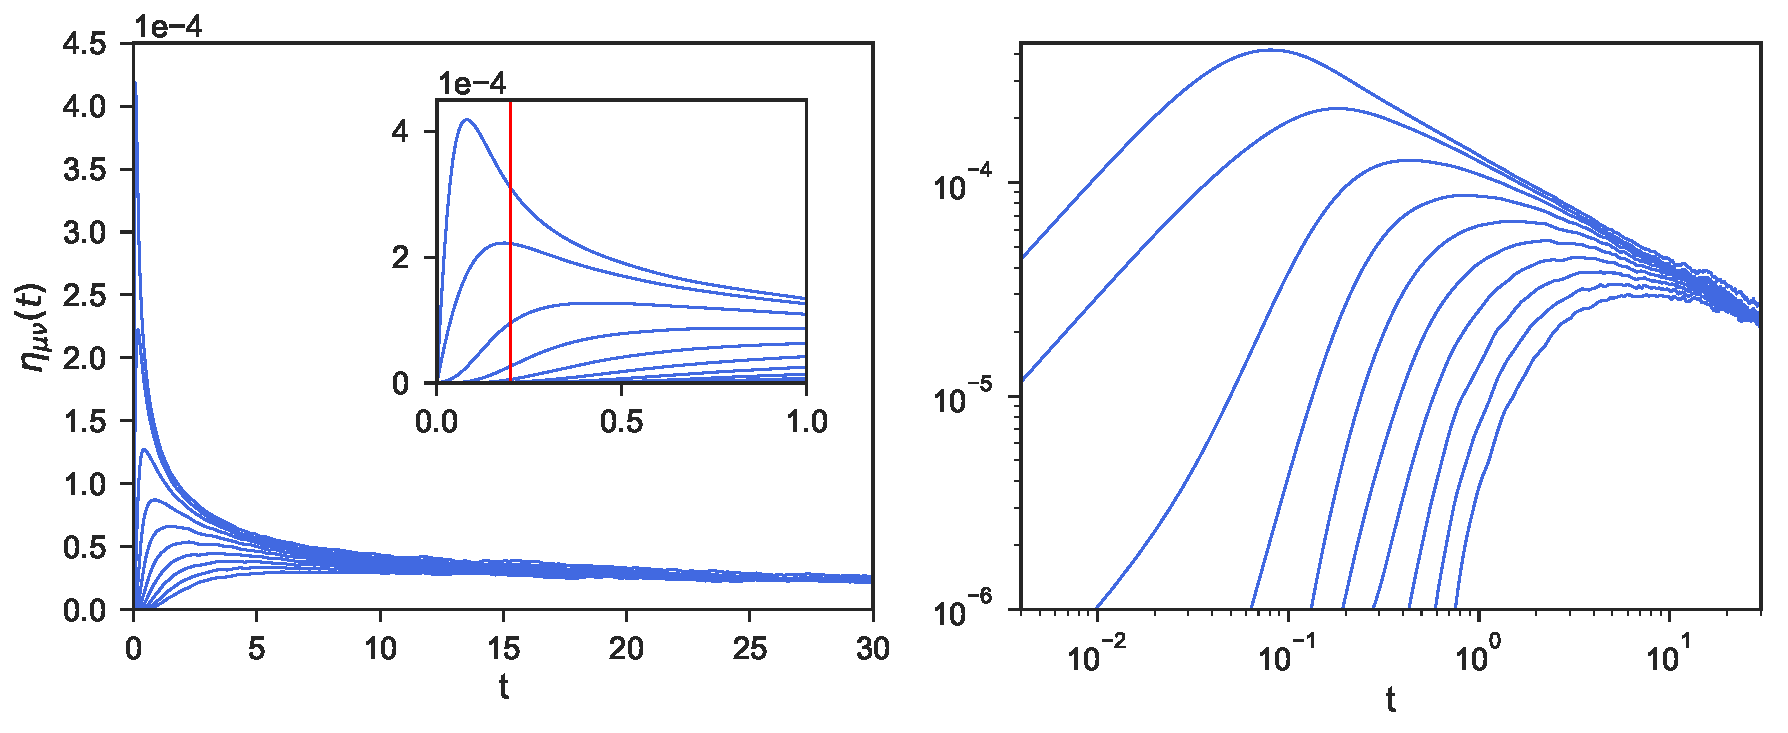
\includegraphics[scale=0.41]{Etat-PBC}
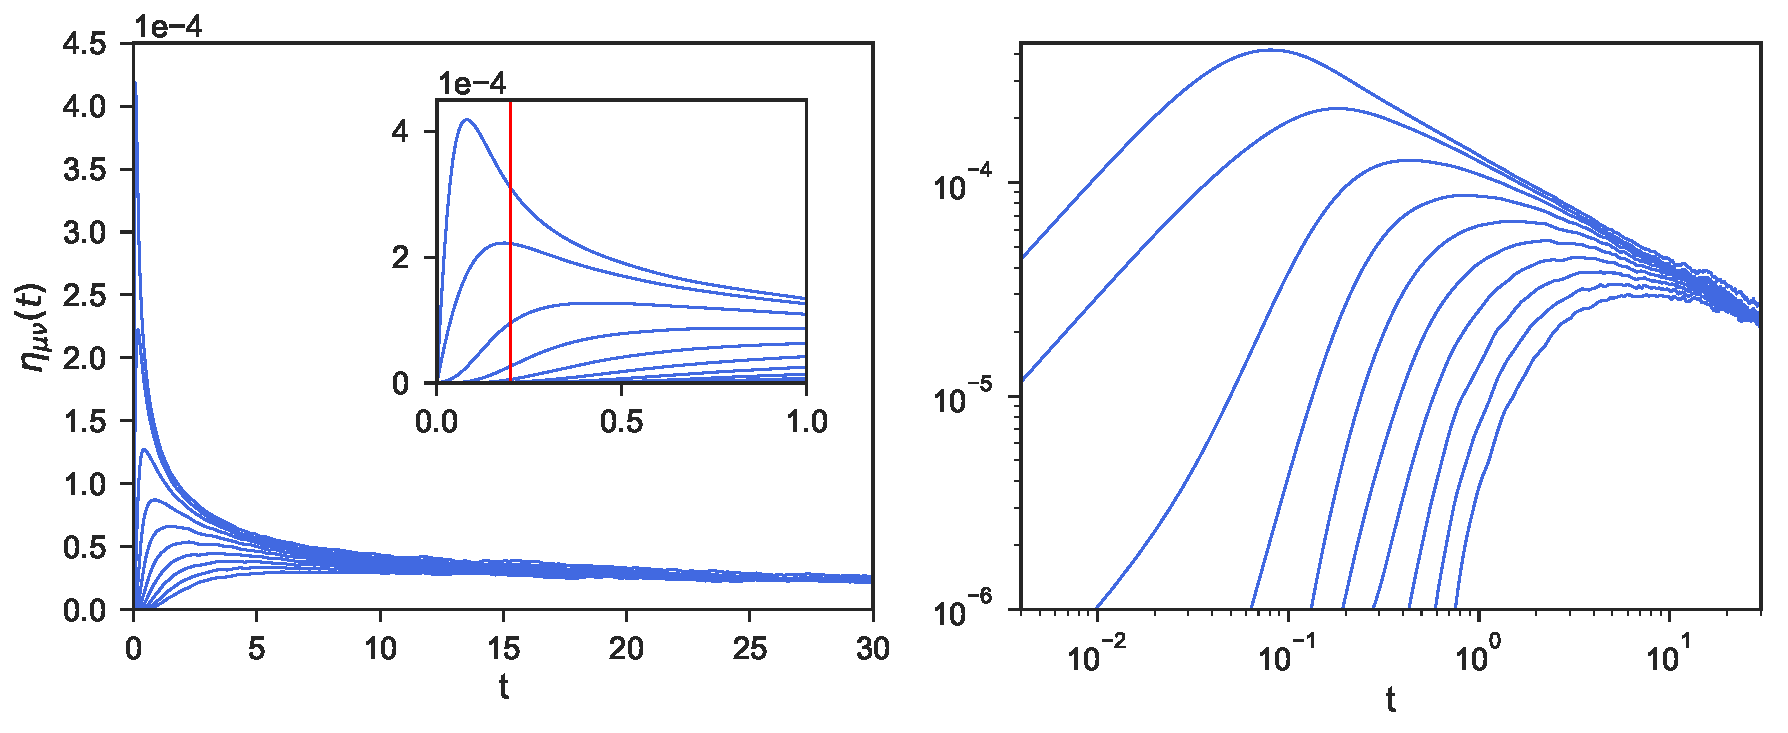
\includegraphics[width=\linewidth]{Etat-PBC}
\caption[The nonlocal viscosity as a function of time for PBC system]{The nonlocal viscosity $\eta_{\mu\nu}(t)$ as a function of time, for $\mu=30$ and, in descending order, $\nu=30-40$. The left panel is in linscale, while the right panel in logscale. The inset is a zoom and the red line is at $t=\tau$.}
\label{fig:Etat-PBC}
\end{figure}


In Fig.
\ref{fig:KinVisc0t-PBC} we plot $\nu_0(t)$  which we recall that
is the sum  of the curves in  the left panel of Fig. \ref{fig:Etat-PBC} divided by the density. We observe  a very neat
plateau.  Of course, the plateau cannot extend indefinitely because of
the  finite number  of terms  involved  in the  sum (\ref{eta00}).  \Note{ Entender bien :We
expect that after  an estimated time of the order  of $L^2/\nu_0$ that
takes the vorticity to diffuse the entire system size the plateau will
curve down.  In our system  this time is  $\sim 600$, well  beyond our
observation  span. After  this  time  we expect  that  the plateau  in
$\nu_0(t)$ will start to decrease due to finite size effects.}
\begin{figure}[h!]
  \centering
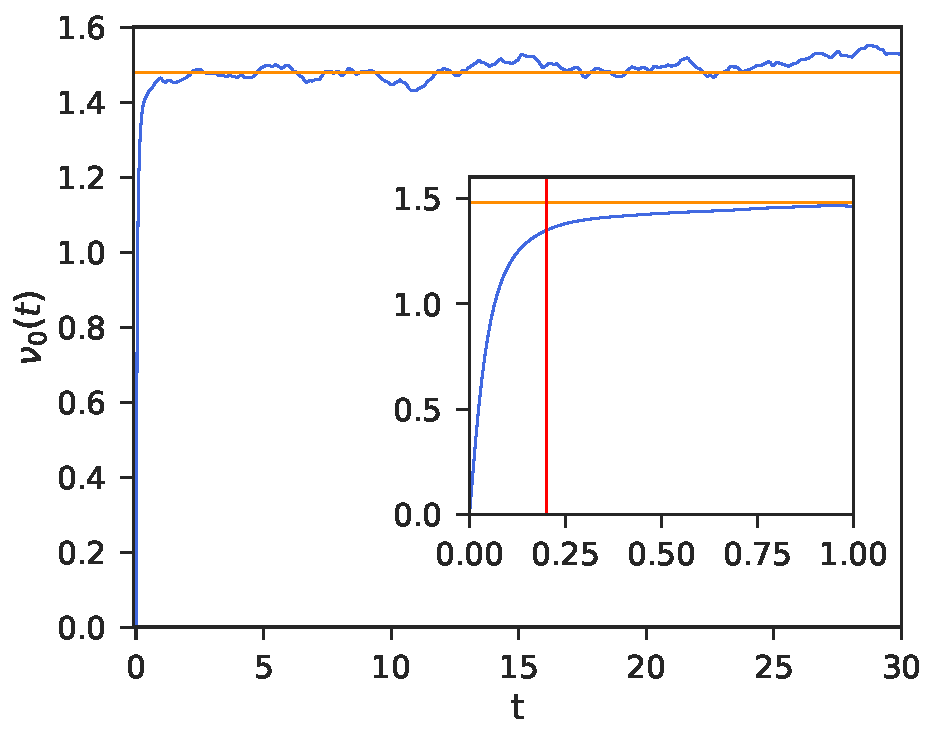
\includegraphics[scale=0.41]{KinVisc0t-PBC}
\caption[The local kinematic viscosity for PBC system]{The local kinematic viscosity $\nu_0(t)=\eta_0(t)/\rho^{\rm eq}$ as a function of time where the shear viscosity is computed with the data from Fig. \ref{fig:Etat-PBC}. A horizontal orange line at $\nu_0=1.48$ from the literature \cite{Woodcock2006} is also plotted in order to guide the eye in the plateau region.}
\label{fig:KinVisc0t-PBC}
\end{figure}

We have shown in  equation (\ref{FouFin}) how to evaluate  the nonlocal shear
viscosity  matrix  $\tilde{\eta}^*_{\mu\mu}$  not  from  the  standard
Green-Kubo  formula but  rather from  a corrected  version of  it that
accounts for the  fact that the Green-Kubo running  integral decays as
the correlation of  the CG variables themselves. 
%In  order to evaluate
%$\tilde{\eta}^*_{\mu\mu}$ we introduce the time dependent eigenvalue
%\begin{align}
%\tilde{\eta}_{\mu\mu}^*(t)&=\frac{\tilde{\eta}_{\mu\mu}(t) }{\tilde{c}_{\mu\mu}(t)}
%\label{FouFint}
%\end{align}
%which, 
According  to equation (\ref{FouFin}), $\tilde{\eta}^{*}_{\mu\mu}$  should have a plateau  if the
Markovian approximation is appropriate.

In    Fig.      \ref{fig:EtaStartFourier-PBC}    we    show     the    function
$\tilde{\eta}^{*}_{\mu\mu}(t)$  as a  function of  time for  the different
modes.   We observe  that, whenever  the  statistics allow  for it,  a
reasonable plateau  is obtained. Therefore,  it is possible  to define
the  nonlocal  shear  viscosity  matrix  $\eta^*_{\mu\nu}$ in real space  from  the
Fourier transform  of the plateau  value $\tilde{\eta}_{\mu\mu}(\tau)$.  
The row $\mu=30$ of the matrix $\eta^{*}_{\mu\nu}$ is shown in Fig. (\ref{fig:CompareEtas-PBC}). We observe that the width is about $~5\sigma$. This is, approximately twice the cutoff distance of the Lennard-Jones potential. 
%This  is shown in Fig.  \ref{fig:CompareEtas-PBC} where the
%diagonal structure  is apparent,  with a width  that has  around $\sim
%5\sigma$.  This  is, approximately  twice the  cutoff distance  of the
%Lennard-Jones potential.  
One way to  explain this width is  by noting
that  the stress  tensor of  a bin,  defined in  (\ref{sbin}) contains
contributions of pairs  of atoms through the fraction  of the distance
between the atoms. Bins which are  at a distance larger than twice the
LJ cutoff radius  do not have any atom  that simultaneously contribute
to the stress tensor in each  bin. Therefore, it is plausible to infer
that the width of the stress correlation is a consequence of the absence
of correlation between the stress through atoms that contribute to the stress
in both bins.
\begin{figure}[h!]
  \centering
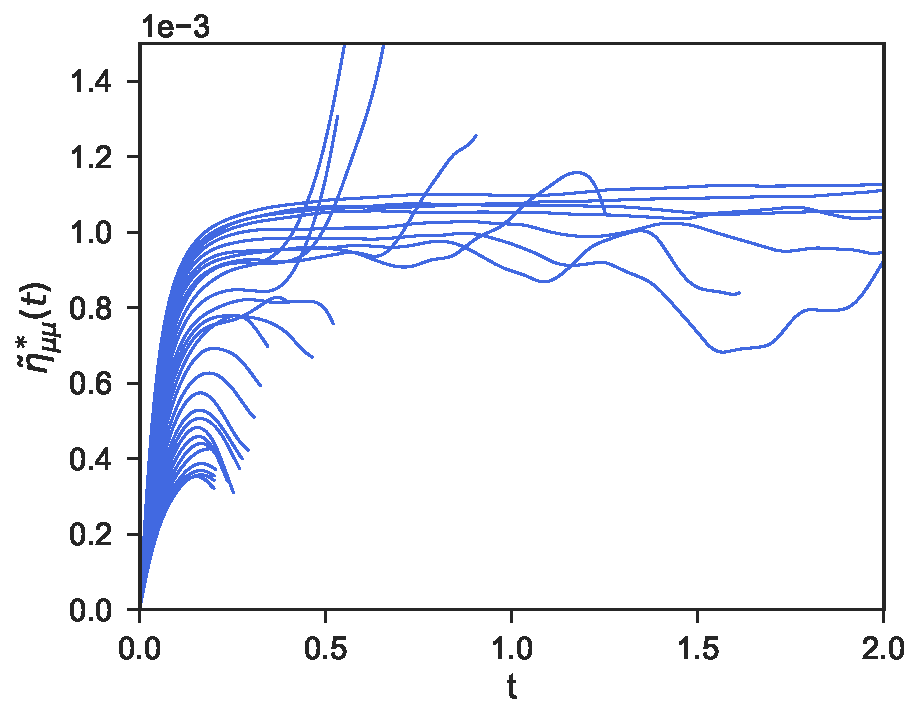
\includegraphics[scale=0.41]{EtaStartFourier-PBC}
\caption[The nonlocal shear viscosity kernel for PBC system]{The nonlocal shear viscosity kernel from corrected Green-Kubo formula $\tilde{\eta}^*_{\mu\mu}=\frac{\tilde{\eta}_{\mu\mu}(t)}{\tilde{c}_{\mu\mu}(t)}$}
\label{fig:EtaStartFourier-PBC}
\end{figure}


\begin{figure}[h!]
  \centering
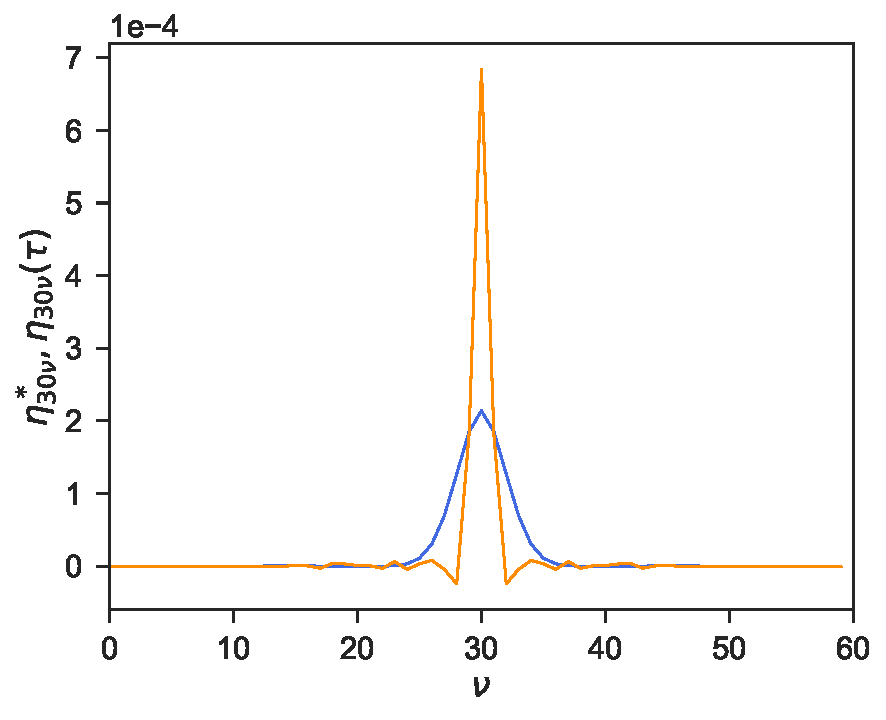
\includegraphics[scale=0.41]{CompareEtas-PBC}
\caption[Comparison $\eta^*_{30,\nu}$ and $eta_{30,\nu}$]{The row $\mu=30$ of the nonlocal shear viscosity matrix $\mu^{*}_{\mu\nu}$ in real space obtained from the corrected Green-Kubo formula (orange) . Also plot is the nonlocal shear viscosity $\eta_{\mu\nu}$ for the Green-Kubo running integral (blue).}
\label{fig:CompareEtas-PBC}
\end{figure}


The kinematic viscosity  in Fourier space is  obtained thought equation (\ref{nustartilde})
%by transforming equation (\ref{numunu0})
%to Fourier space  and gives
%\begin{align}
%\tilde{\nu}_\mu(t)&=  \frac{{\cal V}_\mu \tilde{\eta}_\mu(t)}{\tilde{\rho}_\mu}
%  \label{kinViscFourier}
%\end{align}
We plot $\tilde{\nu}_\mu(t)$  in Fig.  (\ref{fig:KinVisctFourier-PBC}) as a  function of time
$t$ for  different modes  $\mu$ (left)  and as a  function of  the mode
number $\mu$  at different times from $t=0$ to $t=0.2$ in intervals of $0.01$ (right). From
the last plot  we observe that the modes around  $\sim 30$ are subject
to  large statistical  error because  for these  modes the  eigenvalue
$\tilde{c}_\mu(t)$ of  the correlation  matrix has already  taken very
low values, thus  amplifying though its inverse  the small statistical
errors present. In  any case, we observe  that $\tilde{\nu}_\nu(t)$ is
almost constant for all values of $\mu$ and that for times larger than
$\tau=0.2$ the  kinematic viscosity  of all  modes is  fairly constant
$\tilde{\nu}_\nu(\tau)\simeq\nu_0=1.48$  in  reduced units.  This  is,
another reflection  of the  fact that the  discrete hydrodynamics in 
periodic boundary conditions is fairly local, and can be described with
 a local in space approximation, as has been corroborated in Figs. 
 \ref{fig:Predictionsmumu-PBC}, \ref{fig:Predictionsmumu+1-PBC} and \ref{fig:EtaStartFourier-PBC}.


\begin{figure}[h!]
  \centering
%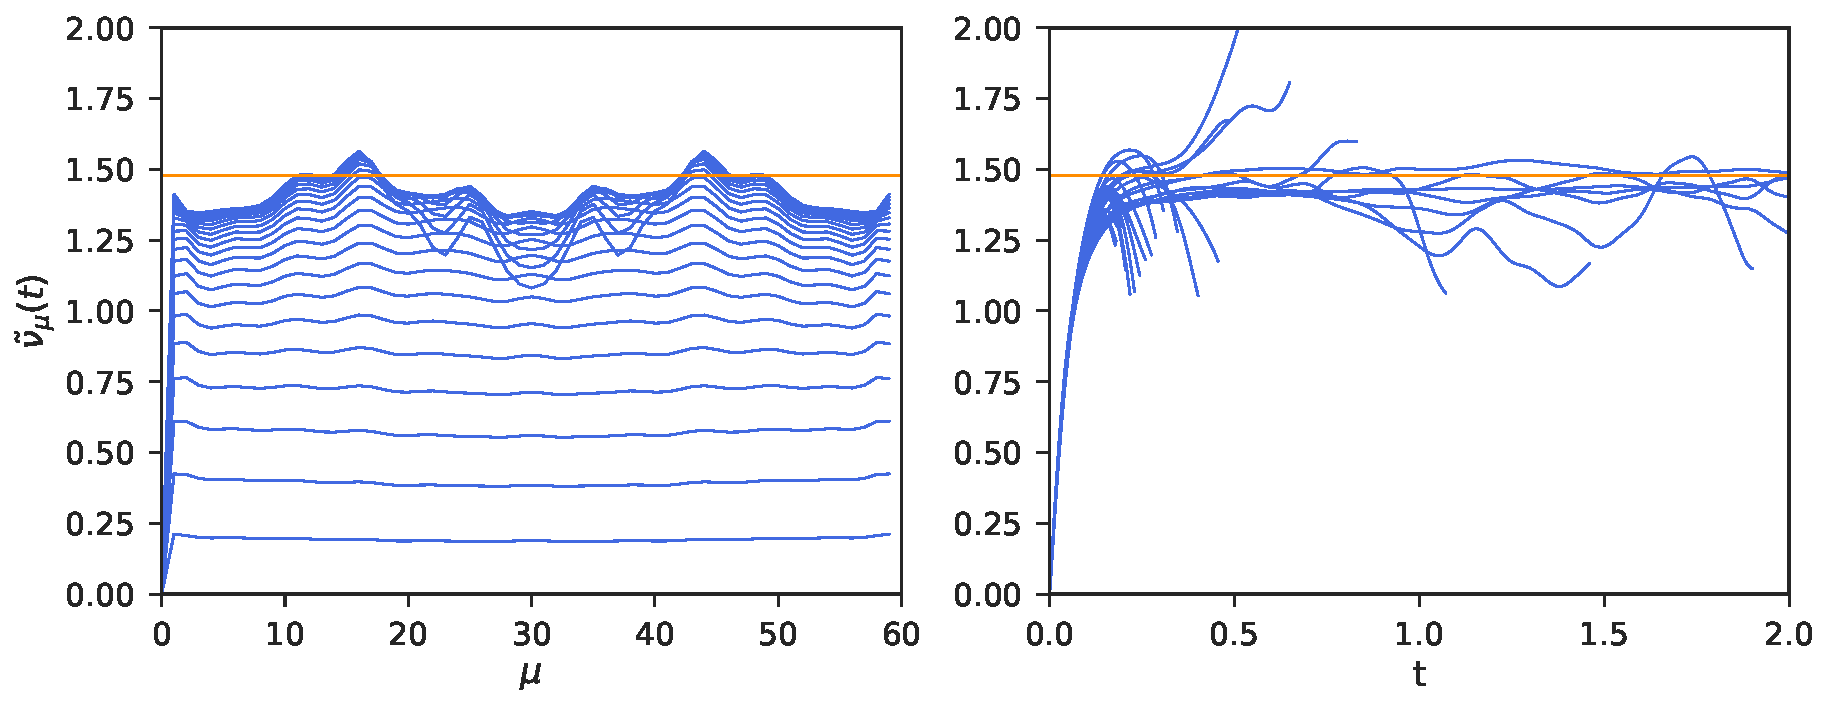
\includegraphics[scale=0.41]{KinVisctFourier-PBC}
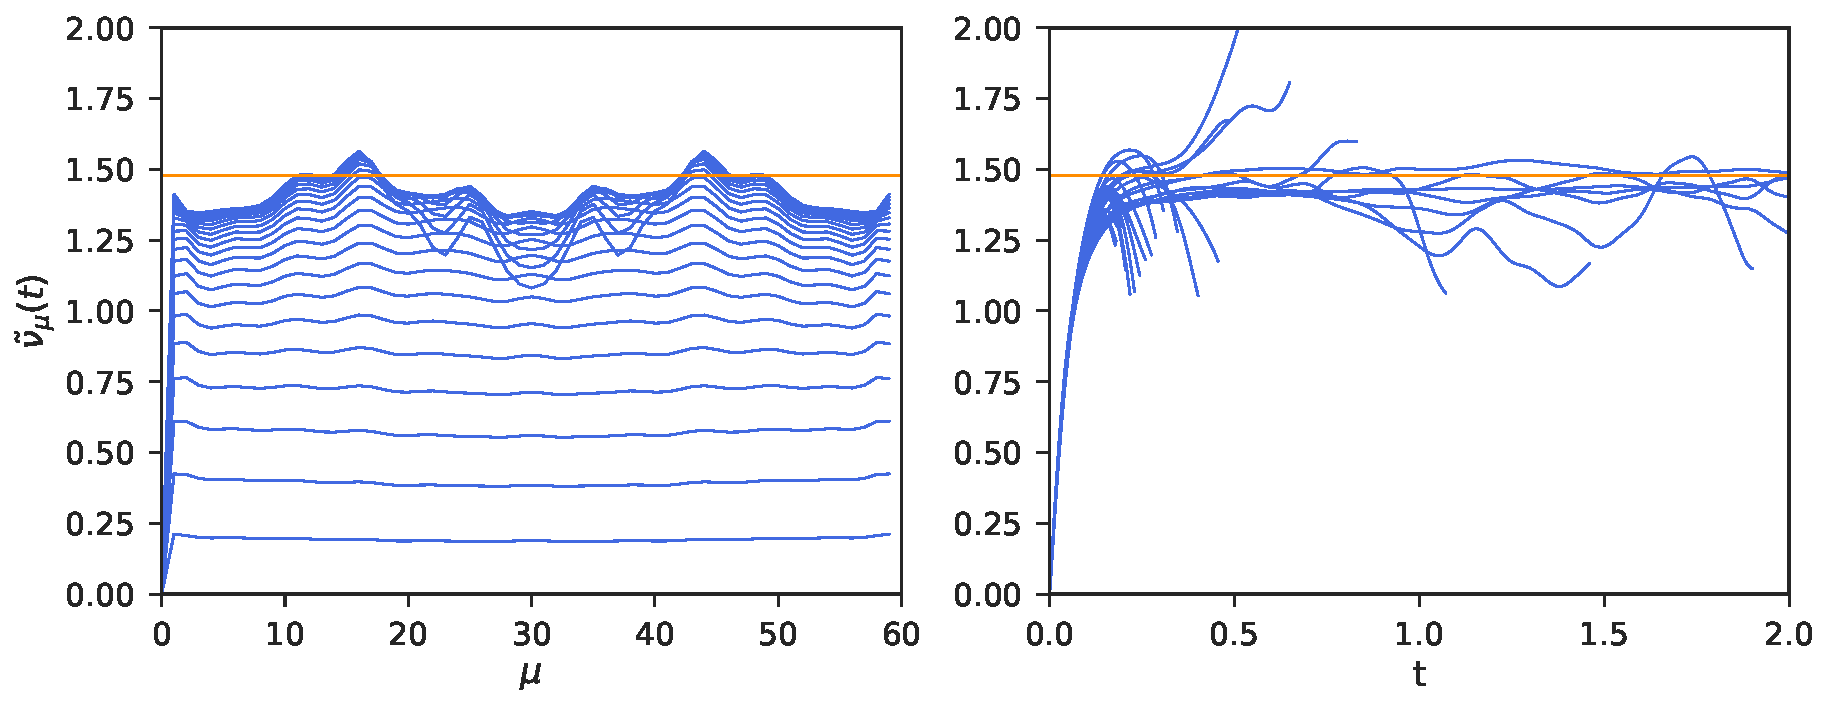
\includegraphics[width=\linewidth]{KinVisctFourier-PBC}
\caption[The eigenvalues of the nonlocal kinematic viscosity matrix for PBC system]{The eigenvalues of the nonlocal kinematic viscosity matrix defined in equation (\ref{kinViscFourier}) as a function of time (right panel), and as a function of the mode index por times from t=0 to t=0.2 in ascending order in intervals of $0.01$. The orange line at $\nu_0=1.48$ is plotted in order to guide the eye in the plateau region.}
\label{fig:KinVisctFourier-PBC}
\end{figure}

\newpage
\section{Summary}
\label{Sec:SummaryChapPBC}
In this chapter we have addressed the plateau problem that appears in
the  expression of  transport  coefficient in  terms  of the  standard
Green-Kubo running integrals.  In the  case of Markovian dynamics with
not an extreme separation of time  scales, the decay of the Green-Kubo
running integral does  not allow to determine  unambiguously the value
of the  transport coefficients.  We  have shown in  equation  (\ref{Math1})
that  the  Green-Kubo  running  integral necessarily  decays  to  zero
because it  is given in terms  of the correlation of  the CG variables
and its  time derivative.  With  this observation, we have  proposed a
correction  to  the  standard  Green-Kubo  expression  that  does  has  a
well-defined infinite time limit. 

After that we have introduced the Mori theory for discrete hydrodynamics and we  have computed from  MD simulations  the equilibrium
time-dependent correlation matrix of  the discrete transverse momentum
density.   Under  the Markovian  approximation,  Mori  theory gives  a
definite prediction for the correlation  matrix in terms of a decaying
matrix exponential.   As we  have discussed, the  Markovian prediction
\textit{cannot}  hold for  very small  times, essentially  because the
exponential matrix decay predicts a  non-zero value of the derivatives
of the correlation at  $t=0$, while microscopic reversibility enforces
a  vanishing value  of the  derivative of  the correlations  at $t=0$.
Therefore,  the initial  decay of  the  correlation cannot  be of  the
exponential matrix form.  Only after a time $\tau$ in which the memory
has fade out one can expect  a Markovian, local in time, approximation
to hold.   We have  observed that  the relaxation  matrix $\Lambda(t)$
does indeed plateau  to a constant value  $\Lambda^*$, indicating that
after  the  time  $\tau$  the  decay  of  the  correlation  matrix  is
exponential  and hence  Markovian.   At the  plateau  time $\tau$  the
correlation matrix has decayed already to 50\% of its initial value.

The  \textit{nonlocal}  shear  viscosity  defined  in  terms  of  the
Green-Kubo  formula   as  the  time  integral   of  the  stress-stress
correlation does not show a plateau.  Quite remarkably, the sum of the
(non-plateau) nonlocal  shear viscosity  matrix elements  does indeed
have  a  plateau.   This  plateau corresponds  to  the  \textit{local}
viscosity computed in  the usual way from its  Green-Kubo formula. The
existence of  this plateau  in the  local viscosity  is due  to global
momentum  conservation.  By  using the  nonlocal viscosity 
once corrected  according to the  method in Sec. \ref{Sec:GKsi}, we  observe that
the predictions for  the correlation matrix $C(t)$  are quite accurate
even for times smaller than the  plateau time $\tau$. In this way, the
nonlocal model describes  the behaviour of the  correlation matrix in
real space for  very small times, during the decay  of the correlation
from 80\% its  initial value on. We observe that  for the times beyond
$\tau$ in which the Markovian  (local in time) approximation is valid,
the  local in  space approximation  of the  kinematic shear  viscosity
matrix gives already very accurate results.
In  summary, the  eigenvalues of  the  correlation matrix  decay in  a
strict exponential  way, signaling  Markovian behaviour, after  a time
$\tau=0.2$. 
%In real  space, the Markovian  approximation with
%the nonlocal  viscosity $\eta^*$ gives already  very good predictions
%for much shorter times of the order $t=0.07$.

One strategy to increase the validity of a purely Markovian theory for
times   smaller  than   $\tau$   consists   on  including   additional
non-conserved variables in the list  of CG variables.  For example, by
including the stress tensor and heat flux as additional variables, one
expects  to  capture the  viscoelastic  and  memory effects  that  are
required to describe the dynamics  of the conserved variables at smaller
time scales \cite{Khayat1989,Mryglod1995,Bryk2010}.

In  the  present chapter  we  have  limited  ourselves to  the  discrete
transverse  momentum   variable.   With  the  same   methodology,  the
extension  to   the  rest  of  conserved   hydrodynamic  variables  is
straightforward. We have considered an
unconfined simple fluid  in periodic boundary conditions.  In the next
chapters, the same methodology used here will be used for
the  case of  fluids confined  in between  parallel solid  walls.  The
computational burden in  that case is much  larger because translation
invariance cannot be used in order  to increase statistics, as we have
done  in  the present  chapter.   In  addition  to the  nonlocal  shear
viscosity, new transport coefficients related  to friction and slip at
the wall appear in confined fluids,  as has been recently described in
Ref. \cite{Camargo2018} and in Chapter \ref{Chap:Planar}.



%-----------------------------------------------------------------
% CHAPTER 5
%-----------------------------------------------------------------
\chapter{Markovian behaviour near solids}\label{Chap:Walls}
\markboth{Markovian behaviour near solids}{}
\epigraph{\textit{It's the things we forget about that tell us who we are.}}{Zero K \\ DON DELILLO}
\section{Introduction}
In Chapter \ref{Chap:PBC} we have demonstrated
through MD simulations that the Markovian assumption
is  valid  for  the  description   of  correlations  of  the  discrete
transverse momentum \textit{beyond} certain  time.  We have shown that
beyond  this   time,  hydrodynamics  is  essentially   local  in  time
\textit{and} space.  
In this chapter we follow the same strategy as for unconfined fluids in order to study the Markovian behaviour of a fluid in between two solid slabs. 


As we mentioned in the Introduction, at nanoscopic scales,  a fluid
starts displaying its  molecular structure in phenomena  like the wall
ordering.   In  addition, slip  of  the  fluid  at the  walls  becomes
noticeable.   The  usual  local hydrodynamic  description  with  local
transport coefficients  and no  slip boundary  conditions needs  to be
adequately modified in  order to address the  peculiar fluid behaviour
at  nanoscales. 
%Slip  at nanoscales  has  received a  large amount  of
%attention from the simulation point  of view since the pioneering work
%of Thomson and Robins \cite{Thompson1990,Koplik1995,Troian1997}.

We  have presented  in  Chapter \ref{Chap:Theory}  a  derivation of  the
equations of hydrodynamics in the  presence of solid walls that govern
the  averages of  the  mass  and momentum  density  fields. A  crucial
feature of this theory is that the effect of the walls on the fluid is
not through boundary conditions but  rather through forces confined to
the vicinity  of the solid wall.  In a recent work, Camargo et al. \cite{CamargoBC2018} show  how  boundary  conditions  can  be  derived  when  the  flows  are  of
macroscopic  character.  The  theory  gives  the usual  Navier  slip
boundary  condition  with   microscopically  defined  parameters  that
coincide      with      those      of     Bocquet      and      Barrat
\cite{Bocquet1994}.

The only crucial  assumption made in the formulation of  the theory in
Chapter \ref{Chap:Theory} is  that the dynamics  is Markovian, this  is, that
the hydrodynamic equations do not  have integral memory terms.  It is,
therefore, important to test through MD simulations that the Markovian
approximation is  correct.  Comparison with MD  simulation require the
introduction  of discrete  equations. To  achieve this  goal, we  have
proposed in Chapter \ref{Chap:Planar} a  discrete hydrodynamic theory  for planar
flows near  solid walls  that can  be understood  as a  finite element
discretization of  the continuum  theory presented in Chapter \ref{Chap:Theory}.
The size of the bins enter  the discrete theory as an intrinsic length
scale. The forces on fluid elements are due to the effect of nonlocal
stress tensor and nonlocal surface forces due to the walls.

In the  theory presented in Chapter \ref{Chap:Theory}, based  on the
projection  operator technique,  the Markovian  approximation produces
formal expressions in  terms of Green-Kubo formulas  for the transport
coefficients.    However,  these   expressions  are   formal  for   two
reasons. First they involve the  so called projected dynamics which is
uncomputable from MD  simulations. The usual step  of substituting the
projected dynamics  by the real  Hamiltonian dynamics is  not entirely
justified. The second  problem is that the  Green-Kubo formulas suffer
from the plateau problem \cite{Kirkwood1949,Espanol1992}.  
In Sec. \ref{Sec:GKsi} we have  presented a   new  corrected   Green-Kubo  expression   for  transport
coefficients that does not suffer from the plateau problem.

The  theory presented  in Chapter \ref{Chap:Theory} describes  the
evolution of nonequilibrium ensemble averages  and it is based on the
Kawasaki-Gunton  projector \cite{Grabert1982}.   It is  nonlinear and
involves the  free energy functional familiar  from DFT.  For the case of  the transverse momentum, the Kawasaki-Gunton
projector gives  a very simple  linear equation that does  not involve
the free  energy functional.   A very similar  linear equation  can be
obtained  in an  alternative way  from the  simpler Mori  theory, that
always produces  linear equations.   In order  to address  the plateau
problem  it proves  very  convenient to  have a  theory  not only  for
averages but also for time correlation functions and both are provided
in Mori theory.  


\section{The CG variables and its dynamics}

\label{Sec:CGWALLS}
We  consider a  Lennard-Jones  fluid system  confined  in between  two
parallel solid walls made of Lennard-Jones particles fixed in a simple
cubic lattice. The  walls are along the directions  $x,y$.  Because of
traslational invariance along the walls, we bin the vertical direction
$z$ in  layers paralel to the  planar walls.  The box  length $L_z$ is
divided in $N_{\rm bin}$ bins labelled  with an index $\mu$.  The bins
are separated by $N_{\rm bin}$  nodes (actually, nodal planes) located
at  $z_\mu=\mu \Delta  z$, $\mu=0,\cdots,N_{\rm  bin}-1$, with  $\Delta
z=L_z/N_{\rm  bin}$.   We  assume   that  we  have  periodic  boundary
conditions in  the $z$ direction,  albeit due  to the solid  walls the
fluid will never cross the  periodic boundary nor interact with itself
through the  boundary conditions as the  width of the walls  is larger
than the  cutoff of  the interaction potential.   The node  $\mu=0$ is
equal to  the node  $N_{\rm bin}$.   
%We carefully  distinguish between
%\textit{nodes} and  \textit{bins}: nodes are  points in the  $z$ axis,
%while bins are segments in this  axis.  In 3D, nodes are planes, while
%bins are slabs.  As it will  become apparent, from a microscopic point
%of view, mass, momentum, and force densities are defined at the nodes,
%while  stress  is  defined at  the  bins.   Each  bin  is a  layer  of
%dimensions  $L_x,L_y,\Delta  z$.    We  introduce  the  characteristic
%function of  the bin  $\chi_\mu({\bf r})$  that takes  the value  1 if
%${\bf r}$  is in the bin  and zero otherwise.  The  volume integral of
%the   characteristic  function   gives  the   volume  ${\cal   V}_\mu=
%L_xL_y\Delta  z$  of the  bin.   As  discussed  in Chapter   \ref{Chap:Planar}  we
%introduce the  finite element  basis function $\Phi_\mu({\bf  r})$ and
%the discrete Dirac $\delta$ function
%\begin{align}
%\delta_\mu({\bf r})&=\frac{\Phi_\mu({\bf r})  }{{\cal V}_\mu}
%  \label{delta}
%\end{align}

In this chapter,  we use as the only CG  variable relevant to the
problem  the parallel  component  $\hat{g}_\mu={\bf  g}_\mu^x$ of  the
momentum density field defined microscopically as
\begin{align}
\hat{\bf g}_\mu&=\sum_i{\bf p}_i\delta_\mu({\bf q}_i),
\end{align}
where $\delta$ is the discrete Dirac $\delta$ function defined in (\ref{DelFE}).

We   have   checked   that   the   correlations   $\llangle   \hat{\bf
  g}^x_\mu(t)\hat{\bf     g}^z_\nu\rrangle$,    $\llangle     \hat{\bf
  g}^x_\mu(t)\hat{\rho}_\nu\rrangle$     are    vanishingly     small,
corroborating  the predictions  of the  theory. Therefore,  as far  as
shear motion of  the fluid is concerned, a level  of description given
by the  parallel component  $\hat{\bf g}^z _\mu$ should  be sufficient.
We will consider elsewhere the  more general situation that allows one
to  study compression  of the  fluid in  the direction  normal to  the
walls.

We will  collect the  CG variables  into an  $N_{\rm bin}$-dimensional
column  vector  $\hat{g}$ that  contains  as  components the  parallel
component   of  the   momentum   density  of   bin   $\mu$,  this   is
$\hat{g}^T=(\hat{\bf   g}^x_1,\cdots,\hat{\bf  g}^x_{N_{\rm   bin}})$,
where the superscript $T$ denotes the transpose.  The central quantity
in this chapter is the equilibrium time correlation matrix $C(t)$ of the
CG variables given by
\begin{align}
  C(t)=\llangle \hat{g}(t) \hat{g}^T\rrangle
\end{align}
According  to  Mori  theory  the
correlation matrix decays in a linear way,
\begin{align}
 \frac{d}{dt}C(t)&= -\Lambda^*\esc C(t),
\label{InFull-C}
\end{align}
where  the  relaxation  matrix   $\Lambda^*$  is  a  constant  $N_{\rm
  bin}\times N_{\rm  bin}$ matrix. The relaxation  matrix subsumes all
  the transport coefficients  of the system. As shown  in Chapter \ref{Chap:PBC},
the relaxation  matrix can  be decomposed  into a  nonlocal viscosity
contribution and nonlocal friction contributions, all defined through
Green-Kubo expressions,  suitably corrected  with the method  given in
Sec. \ref{Sec:GKsi}.  As discussed in  Chapter \ref{Chap:PBC} a  Markovian equation
like (\ref{InFull-C}) is expected to hold only after a time $\tau$ has
elapsed.  The reason is that from  the time reversal properties of the
CG  variables we  know that  the  time derivative  of the  correlation
matrix at  $t=0$ vanishes,  but equation   (\ref{InFull-C}) would  imply at
$t=0$ the absurd result $0=-\Lambda^*\esc C(0)$.

The Markovian relaxation equation (\ref{InFull-C}) predicts the following
evolution equation for correlation matrix
\begin{align}
  C^{\rm predict}(t)&=\exp\{-\Lambda^* (t-\tau)\}C(\tau),
\label{Cpredict}
\end{align}
where we  have introduced  the matrix  exponential through  its Taylor
series and have taken into account that equation  (\ref{InFull-C}) can only
be valid after  a time $\tau$. The elements of  the matrix exponential
do not  need to  decay as  exponential functions. As  we will  see, in
fact,  the decay  is  quasi-algebraic.   

In order to have an easier  identification of whether the evolution of
the  matrix  exponential  is   described  by  the  Markovian  equation
(\ref{InFull-C}) it  proves convenient to diagonalize  the correlation
matrix.   We introduce  eigenvalues  $\tilde{C}_\mu$ and  eigenvectors
$u_\mu$ in such a way that  the correlation matrix is given by the
spectral decomposition
\begin{align}
  C(t)&=\sum_\mu^{N_{\rm bin}}\tilde{C}_\mu(t) u_\mu(t) \otimes u_\mu^T(t)
\label{spectral}
\end{align}
The unitary matrix $E(t)$ that  has as columns the eigenvectors allows
to diagonalize the correlation matrix, this is
\begin{align}
  E^{-1}(t)\esc C(t)\esc E(t)=\tilde{C}(t),
\label{diag}
\end{align}
where $\tilde{C}(t)={\rm Diag}[\tilde{C}_1(t),\cdots,\tilde{C}_{N_{\rm
    bin}}(t)]$ is a diagonal matrix  containing the eigenvalues in the
diagonal.   If  the  system  was traslation  invariant  in  the  $z$
dimension, the  matrix $E(t)$ would  be given by  the time-independent
discrete Fourier  transform, as discussed  in Sec. \ref{Sec:Fourier}.   In the
present problem where the solid walls break traslation invariance, the
unitary  matrix  $E(t)$ is  time  dependent.   As a  consequence,  the
diagonal matrix $\tilde{C}(t)$ evolves according to
\begin{align}
\frac{d}{dt}  \tilde{C}(t)&=-\tilde{\Lambda}^*\esc \tilde{C}(t)
  +\frac{d }{dt}(E^{-1}(t)) \esc C(t)\esc E(t)
  +E(t)\esc C(t)\esc \frac{d }{dt}E(t)  
\label{dc}
\end{align}
We have  observed that the  time dependence  of the unitary  matrix is
very weak, $\dot{E}\simeq 0$ and allows one to approximate equation (\ref{dc}) as
\begin{align}
\frac{d}{dt}  \tilde{C}(t)&\simeq-\tilde{\Lambda}^*\esc \tilde{C}(t),
\label{Ctilde}
\end{align}
where,   consistently,  the   matrix  $\tilde{\Lambda}^*$   has  small
off-diagonal elements.   Therefore, we  arrive at the  conclusion that
the eigenvalues  $\tilde{c}_\mu(t)$ of  the correlation  matrix evolve
according to a single exponential
\begin{align}
  \tilde{C}_\mu(t)&=\exp\{-\tilde{\Lambda}_{\mu\mu} (t-\tau)\}  \tilde{C}_\mu(\tau),
\end{align}
where we have  taken into account that the  Markovian approximation is
valid  only  after the  time  $\tau$.  The  exponential decay  is  one
signature    of   the    validity    of    the   Markovian    equation
(\ref{InFull-C}). Another  signature of the validity  is obtained from
each component of (\ref{Ctilde}) that  shows that the function defined
as
\begin{align}
  \tilde{\Lambda}_{\mu}(t)&\equiv -\frac{1}{{\tilde{C}}_{\mu}(t)}\frac{d{\tilde{C}}_{\mu}}{dt}(t)
\label{LambdatRec}
\end{align}
should,  after  a time  $\tau$  reach  the  constant plateau  value  $
\tilde{\Lambda}_{\mu\mu}^*$.  Note  that the eigenvalues  should decay
exponentially  and,  therefore,  $  \tilde{\Lambda}_{\mu}(t)$ in (\ref{LambdatRec}) is  the
product  of an  exponentially decaying  function and  an exponentially
exploding function. This means that we need high quality statistics in
order  to have  sensible values  for $  \tilde{\Lambda}_{\mu}(t)$.  We
also realize that no matter how good our statistics is, we will always
encounter sufficiently large times where the exponential amplification
of statistical errors render  the function $ \tilde{\Lambda}_{\mu}(t)$
meaningless.


\section{Simulations}
\label{Sec:SimWALLS}
The objetive of this section is to present the simulations we made to measure the matrix of correlations $C(t)$ in order to validate the Markovian aproximation of a confined fluid. 
We follow the strategy presented in Sec. \ref{Sec:SimPBC}. Because the translational invariance is broken for confined fluids, it used, instead of the Fourier basis, the eigenvector basis of $C(t)$. 
We deal with a system in which the space occupied by the fluid is exactly the same as in the case of an unconfined fluid. In the first part of this section the fluid region is divided in bins in which $\Delta z$ is the same as the used in Chapter \ref{Chap:PBC}. In the second part, the size of the bins is doubled. 

\subsection{Simulation set up}
A system of particles interacting  with a LJ potential 
truncated at $\sigma=2.5$ has been simulated with the open source code LAMMPS code \cite{Plimpton1995}. The
box size  is $40\times40\times33$,  the number  of fluid  particles is
$N=28175$ and  the time step  is $0.002$ in reduced  units.  Periodic
boundary conditions are assumed  in all directions.   Two solid
walls in the $xy$ plane confine the fluid as is shown in Fig. \ref{fig:WallsBox}.  The bottom wall is made of
two layers  of LJ  particles located  in a  simple cubic  lattice with
lattice spacing  $\sigma$. The top  wall is made  of two layers  of LJ
particles  in a  similar  cubic  lattice.  The  location  of the  four
crystalline planes  are $z=0,1,31,32$  in LJ units.   Due to  PBC, the
distance between  the layers of  solid particles which are  in contact
with   the  fluid   is  $3\sigma$   beyond  the   cutoff  of   the  LJ
potential. Therefore, the fluid particles occupy a space of $30\sigma$
and  do  not  interact  with  the  periodic  images  in  the  vertical
direction. Note that the space occupied by the fluid is equal to the case exposed in the previous chapter, in which the fluid is unconfined. 
\begin{figure}
    \centering
    %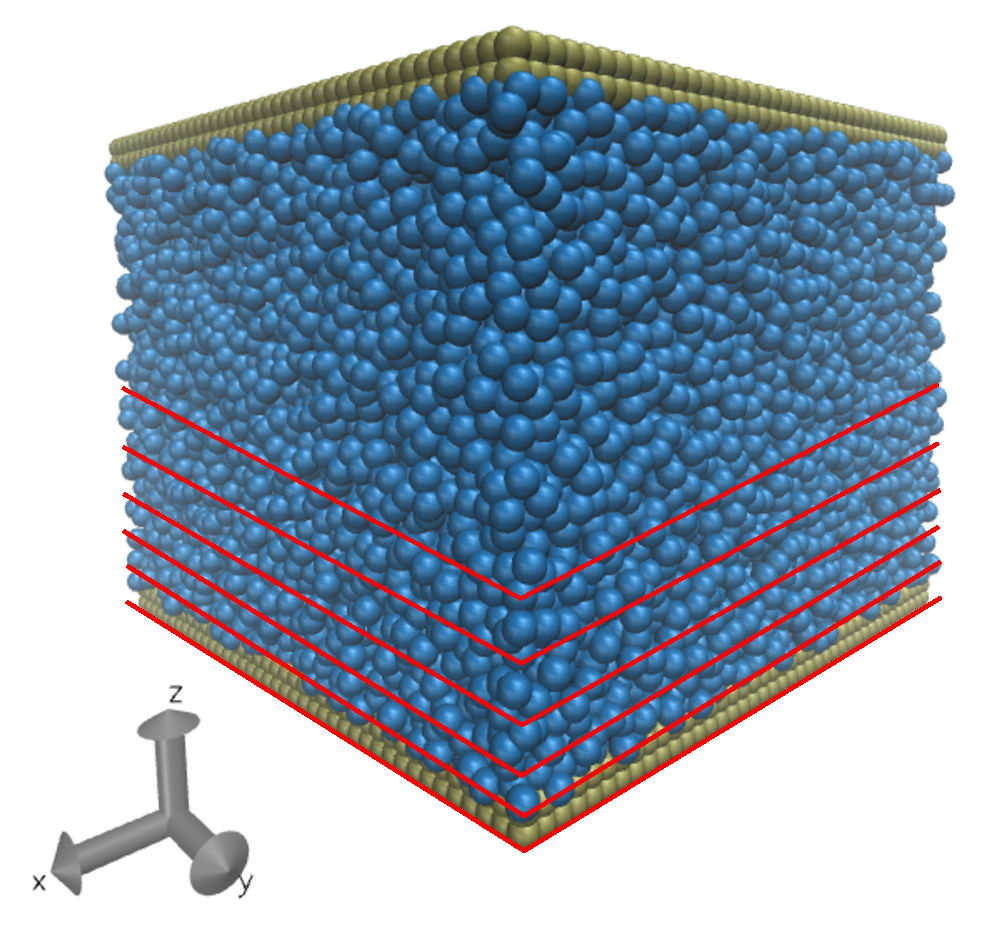
\includegraphics[scale=0.3]{system_nodes_walls}
    \frame{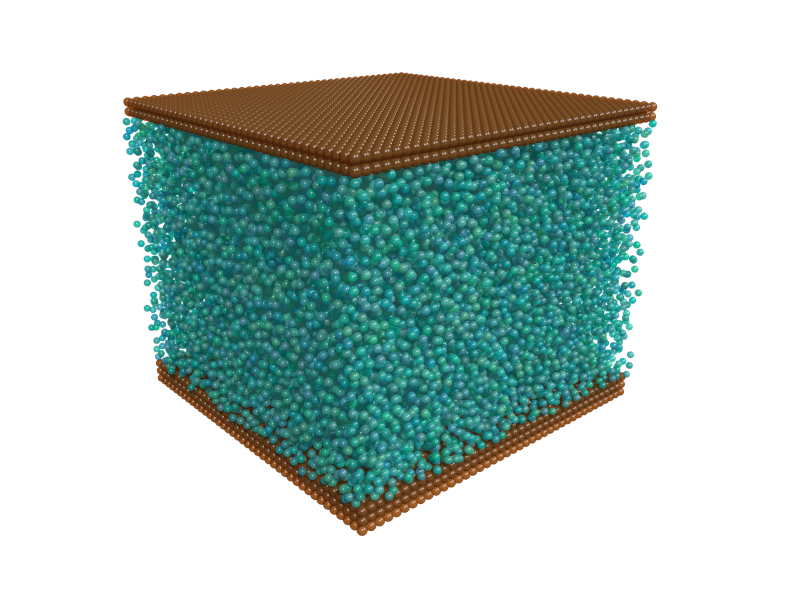
\includegraphics[width=0.45\linewidth]{PRL3_gold2_wo_layers_wo_diffuse}}
    \frame{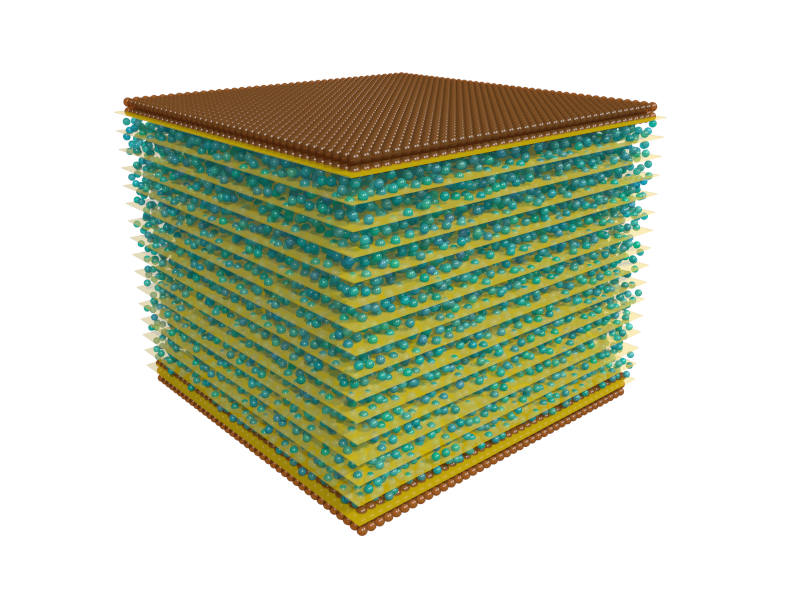
\includegraphics[width=0.45\linewidth]{PRL3_gold2_wo_diffuse}}
    \caption[Walls box]{A visual representation of the MD simulation with a sketch of the binning used. In red are depicted the nodal planes used.}
    \label{fig:WallsBox}
\end{figure}

After an equilibration of $10^5$ timesteps with a Langevin thermostate
to   produce  a   microstate  typical   from  a   thermodynamic  point
corresponding  to  $T=2,\rho=0.6$ in  reduced  units,  the system  is
evolved  under  NVE microcanonical  conditions  for  a further  $10^5$
timesteps.   After  this  equilibration   phase,  production  runs  of
$12\times 10^6$ time  steps are launched and the $x$  component of the
discrete momentum density is recorded  every 2 timesteps.  In order to
increase statistics, we average the result of $18$ simulations.


\subsection{Thin bins with $\Delta z = 0.5\sigma$}
\label{Sec:ThinBins}
The $z$  axis is binned  in $66$ bins of  width of half  the molecular
size, $\Delta z=0.5\sigma$.  The  correlation matrix of the transverse
momentum of different bins is computed, requiring a total of $66\times
66$ time correlations  functions  in each  simulation.   
The support of  the correlation matrix  is extended only  up to a  time of
$t=2$ in reduced units, which  is sufficient to measure the relaxation
matrix $\Lambda(t)$.   A  few  selected  elements of  the  correlation  matrix  are
computed with a very long support of $t=30$ in reduced units, in order
to test the predictions of the theory at long times.

The time correlation  matrix is shown in  Fig.  \ref{fig:Ct-matrix-WALLS-66nodes} at
two different  times, $t=0$ and  $t=0.6$ in  reduced LJ units.   For the
covariance,  at $t=0$,  we can observe the  reminiscense  of the  density
layering near  the wall in the  form of peaks.  As  time proceeds, the
diagonal of  the correlation  widens and  decreases in  height.  Nodes
$\mu=0,1,64,65$ contain  no fluid, while  node $\mu=2,62$ have  a very
small  contribution  from  the  fluid but not negligible.  This means  that  out  of  the
$66\times66$ correlation matrix, we strip off a band of zeros, leaving
a matrix of $61\times61$ nonzero elements.

\begin{figure}[h!]
\centering
%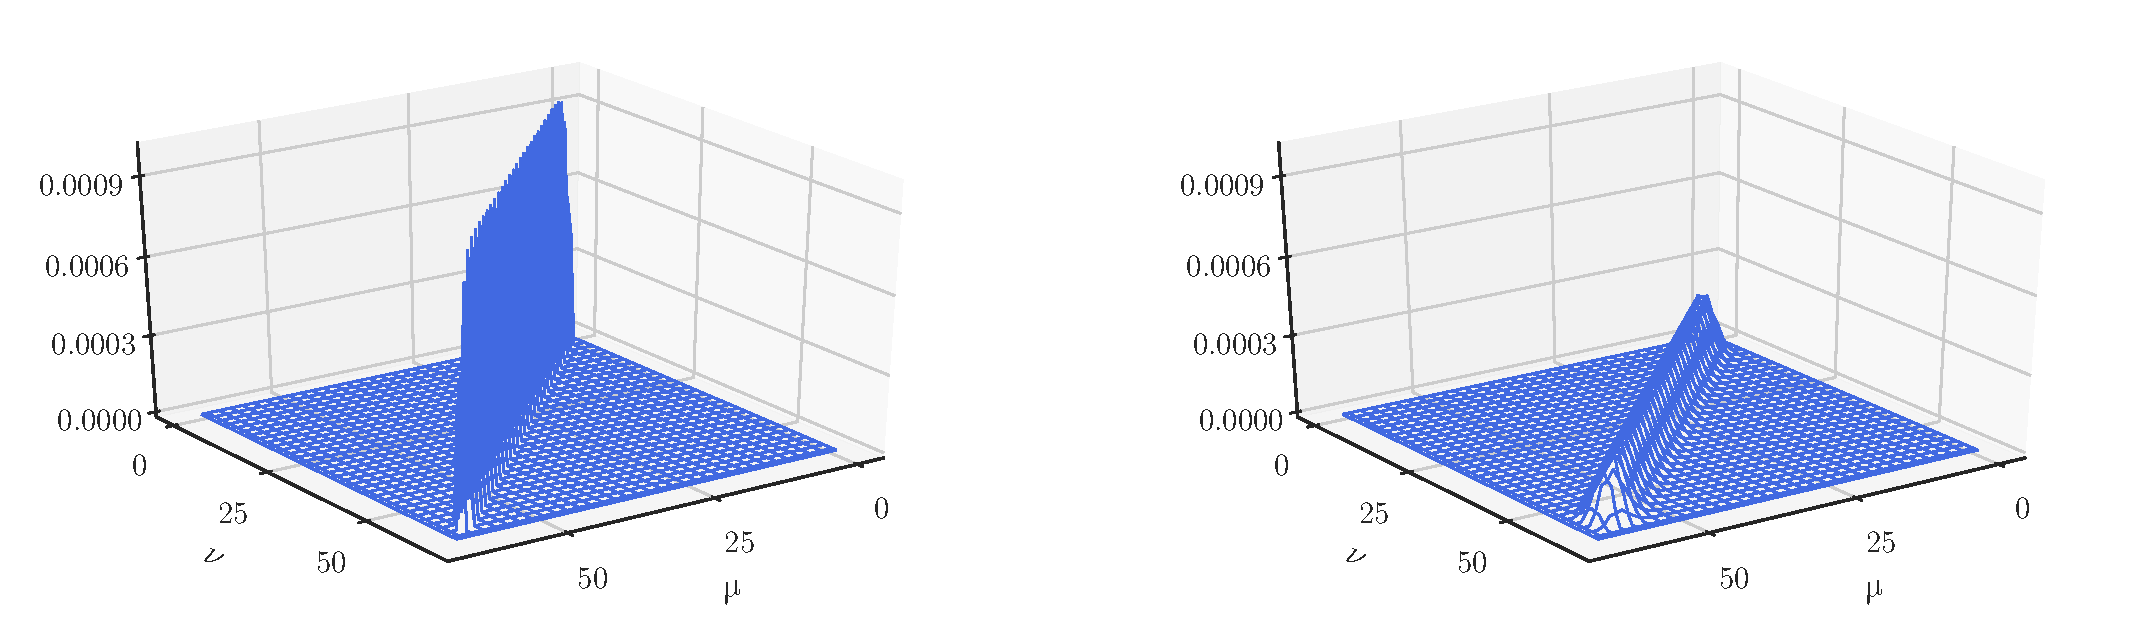
\includegraphics[scale=0.4]{Ct-matrix-WALLS-66nodes}
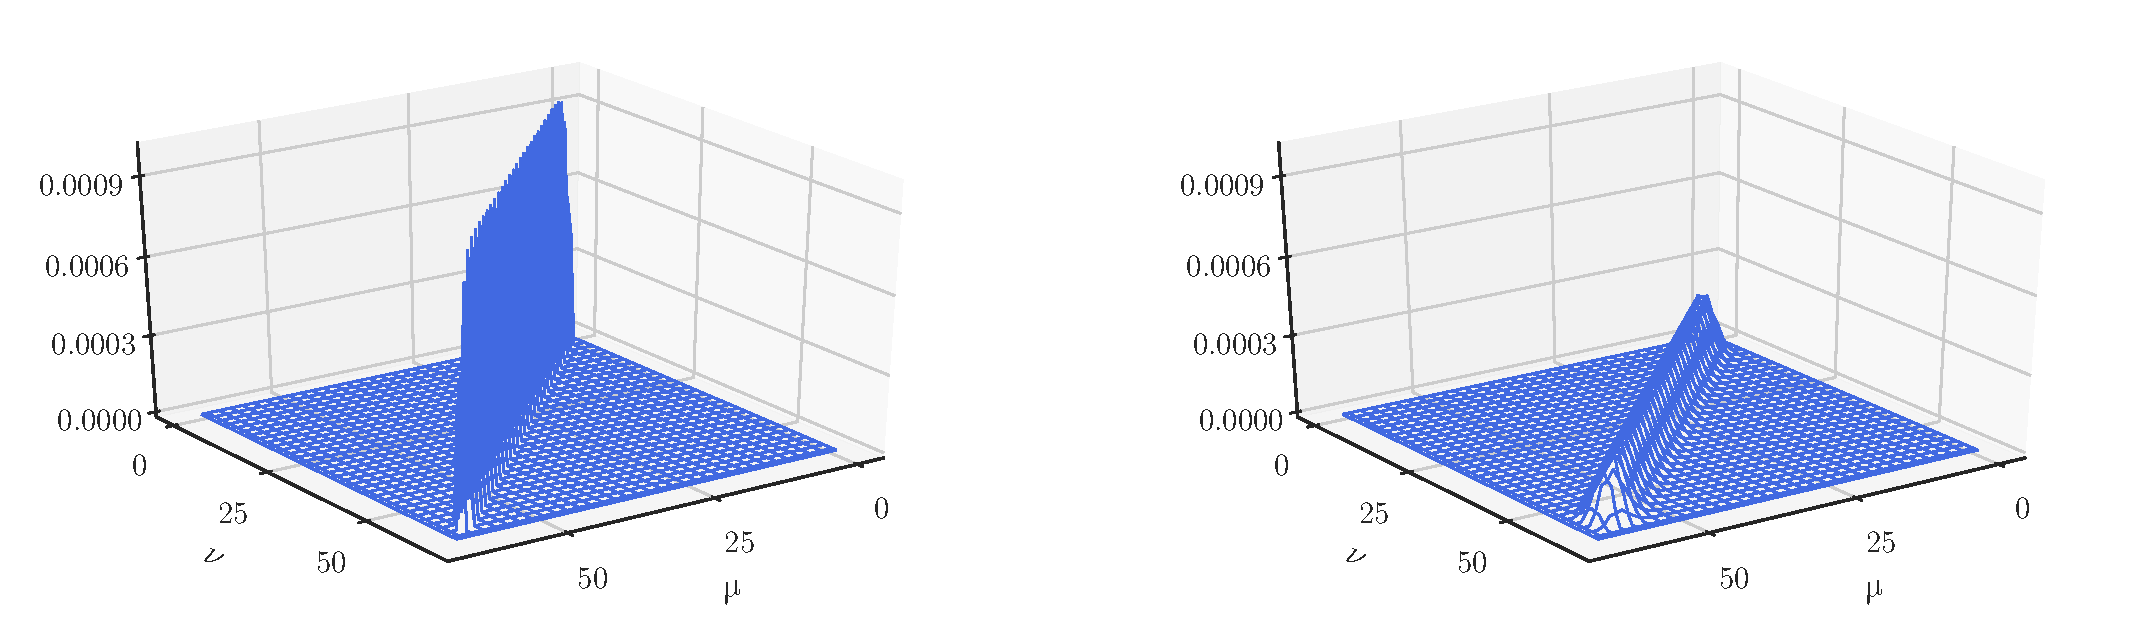
\includegraphics[width=\linewidth]{Ct-matrix-WALLS-66nodes}
\caption[Correlation matrix $C(t)$ at $t=0$ and $t=0.6$ for confined fluid - 66 nodes.]{The   correlation    matrix   $C_{\mu\nu}(t)=\llangle
g_{\mu}(t)  g_\nu\rrangle$ for  $t=0$ (left) and $t=0.6$ (right).}
\label{fig:Ct-matrix-WALLS-66nodes}
\end{figure}

Next, we consider the time-dependent eigenvalues $\tilde{C}_\mu(t)$ of
the correlation matrix $C(t)$.  The eigenvector basis depends slightly
in time. We have checked that by  using the matrix $E(t)$ at the fixed
times  $t=0.15,0.30$  instead  of  the  time-dependent  matrix  $E(t)$  in
(\ref{diag}), the  correlation matrix $C(t)$  essentially diagonalizes
with  the same  eigenvalues,  therefore  validating the  approximation
(\ref{Ctilde}). 
This can be seen in Fig. \ref{fig:LambdatBasis-WALLS-66nodes}, 
where it plotted for clarity only $15$ elements of the diagonal of the matrix $\tilde{\Lambda}(t)$ in three different basis: 
$E(0.15)$, $E(0.30)$ and $E(t)$. 

\begin{figure}[h!]
  \centering
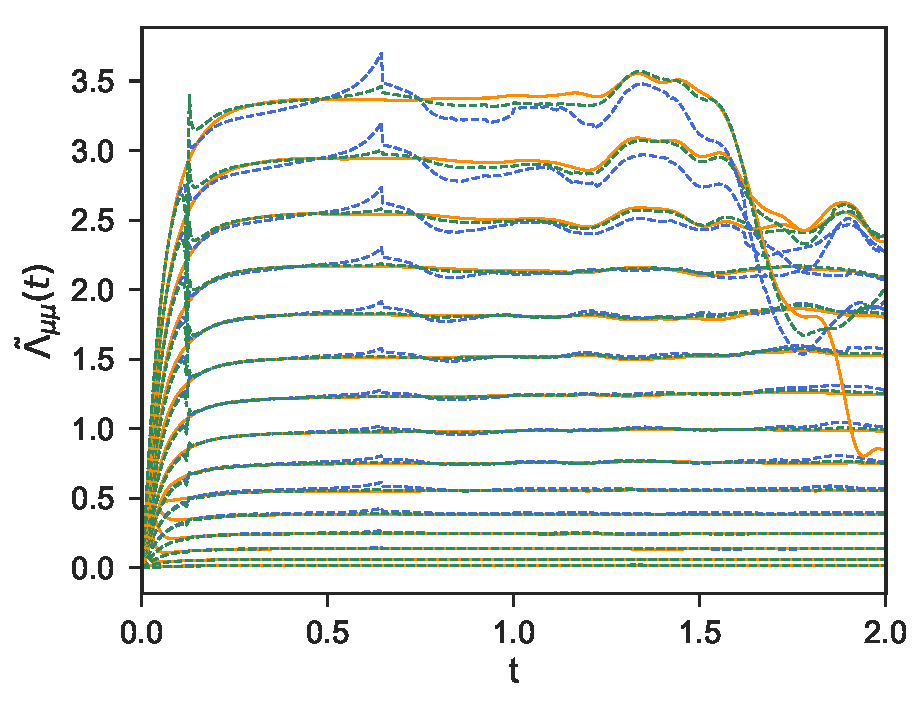
\includegraphics[scale=0.41]{LambdatBasis-WALLS-66nodes}
\caption[Diagonal elements  $\tilde{\Lambda}_{\mu\mu}(t)$ of $\Lambda(t)$ in three different basis - 66nodes.]{The  diagonal elements  $\tilde{\Lambda}_{\mu\mu}(t)$ of  the
  $\Lambda(t)$ in three basis:
$E(0.15)$ (dashed blue lines), $E(0.30)$ (dashed green lines) and $E(t)$ (solid orange lines). }
\label{fig:LambdatBasis-WALLS-66nodes}
\end{figure}


We plot in Fig.  \ref{fig:CtRec-WALLS-66nodes-exp}  all the 61 nonzero eigenvalues, in
descending  order,  as a  function  of  time. Statistical  errors  are
manifest in  the log-lin  plot, in spite  of the  overall high-quality
statistics. Also  clear from the log-lin  plot is the linear  decay of
the eigenvalues  beyond a certain  time, signaled by the  vertical red
line  located at  $\tau=0.2$.   Note that  at  $t=0$ the  correlation
matrix has zero  time derivative due to time  reversal invariance, and
this reflects in the parabolic,  not exponential, initial decay of the
eigenvalues.  In Fig.  \ref{fig:LambdatRec-WALLS-66nodes}  we show
the      function      $\tilde{\Lambda}_{\mu}(t)$      defined      in
(\ref{LambdatRec}). We only plot this  function for the data where the
eigenvalues   $\tilde{C}_{\mu}(t)>2\times10^{-5}$,    which   is   the
horizontal line plotted in the right panel in Fig.  \ref{fig:CtRec-WALLS-66nodes-exp}.  Below this value, which is
two  order  of  magnitude  smaller   than  the  value  at  $t=0$,  the
statistical errors  in the inverse  matrix blow up  exponentially, and
lead to an inverse that varies  erratically and is not reliable.  With
this cutoff,  a very  nice plateau  is observed  for the  lower modes,
reflecting the  exponential decay of  the eigenvalues as shown  in Fig. (\ref{fig:LambdatRec-WALLS-66nodes}).

\begin{figure}[h!]
  \centering
  %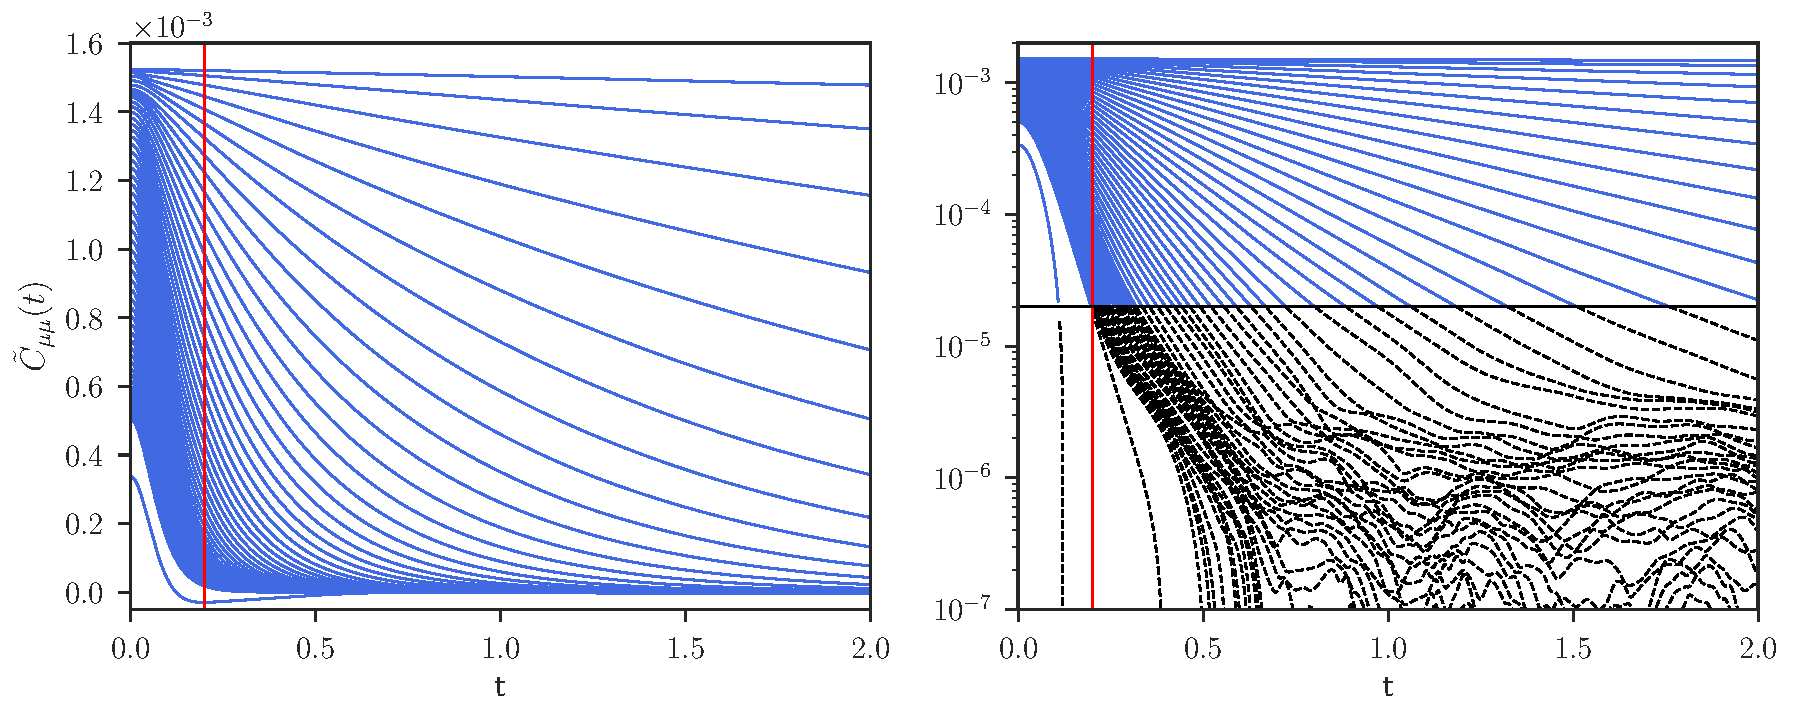
\includegraphics[scale=0.41]{CtRec-WALLS-66nodes-exp}
  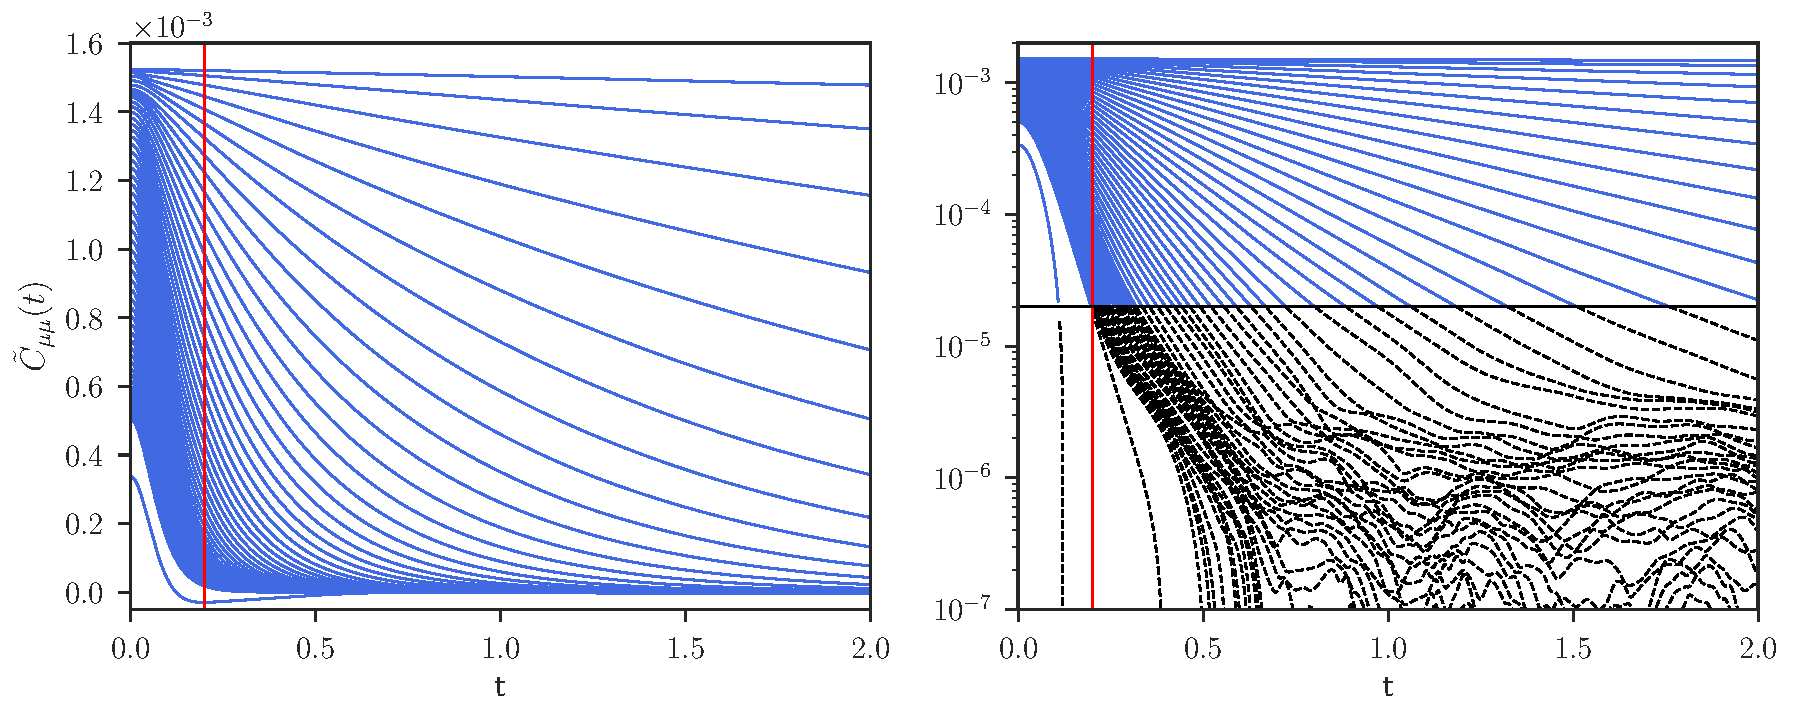
\includegraphics[width=\linewidth]{CtRec-WALLS-66nodes-exp}
  \caption[Evolution of different eigenvalues $\tilde{C}_{\mu\nu}(t)$ for confined fluid - 66 nodes.]{
  The  evolution of  the different
  eigenvalues  $\tilde{C}_{\mu\mu}(t)$ of  the  correlation matrix  of
  momentum  as  a  function  of   time  in  a  lin-lin  plot  (left)
  and   log-lin   plot
  (right). Also  plotted are  a vertical line  at $t=\tau=0.2$  and a
  horizontal  line  at  the   value  $2\times10^{-5}$,  signaling  the
  threshold below which statistical errors give spurious results. }
\label{fig:CtRec-WALLS-66nodes-exp}
\end{figure}

\begin{figure}[h!]
  \centering
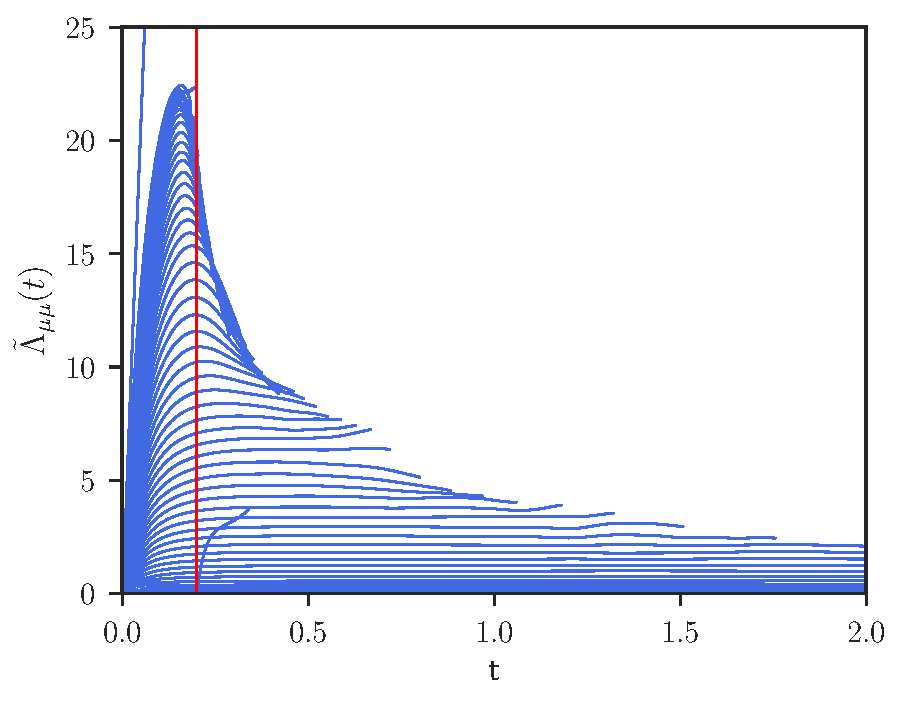
\includegraphics[scale=0.41]{LambdatRec-WALLS-66nodes}
\caption[Diagonal elements  $\tilde{\Lambda}_{\mu\mu}(t)$ of $\Lambda(t)$ in the reciprocal space - 66nodes.]{The  diagonal elements  $\tilde{\Lambda}_{\mu\mu}(t)$ of  the
  $\Lambda(t)$ in the reciprocal space defined in (\ref{LambdatRec}), as a
  function of $t$.}
\label{fig:LambdatRec-WALLS-66nodes}
\end{figure}

One  interesting feature  of the  spectrum of  the correlation  matrix
shown  in  Fig.  \ref{fig:CtRec-WALLS-66nodes-exp}  are  the  smallest two  eigenvalues
corresponding to $\mu=60,61$  that are clearly separated from the rest.
This eigenvalues are plotted in isolation for clarity in the left panel
of  Fig.  \ref{fig:EigenvaluesVectors-WALLS-66nodes}.   Note that  these eigenvalues  have a
distinct negative tail. This implies that  these modes do not decay in
an exponential way at all. The corresponding eigenvectors are shown in
the  right  panel of  Fig.   \ref{fig:EigenvaluesVectors-WALLS-66nodes}.   Note that  these
eigenvectors  are  localised  near   the  walls  and,  therefore,  the
contribution  of this  eigenvectors  into  the spectral  decomposition
(\ref{spectral}) boils  down to  a sort of  bounce-back effect  of the
fluid in the direction parallel to the walls.

\begin{figure}[h!]
  \centering
%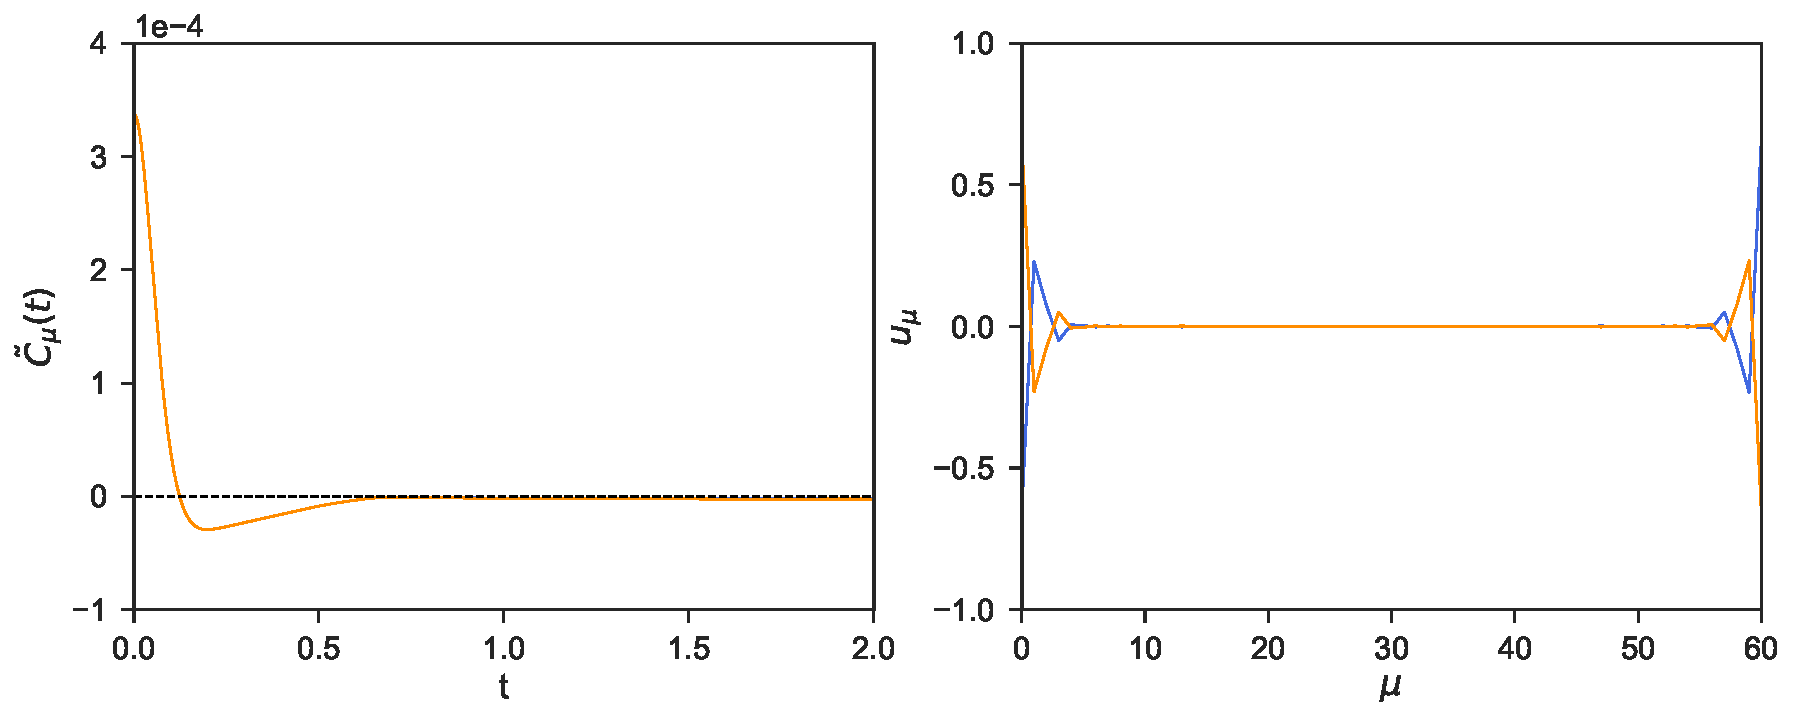
\includegraphics[scale=0.41]{EigenvaluesVectors-WALLS-66nodes}
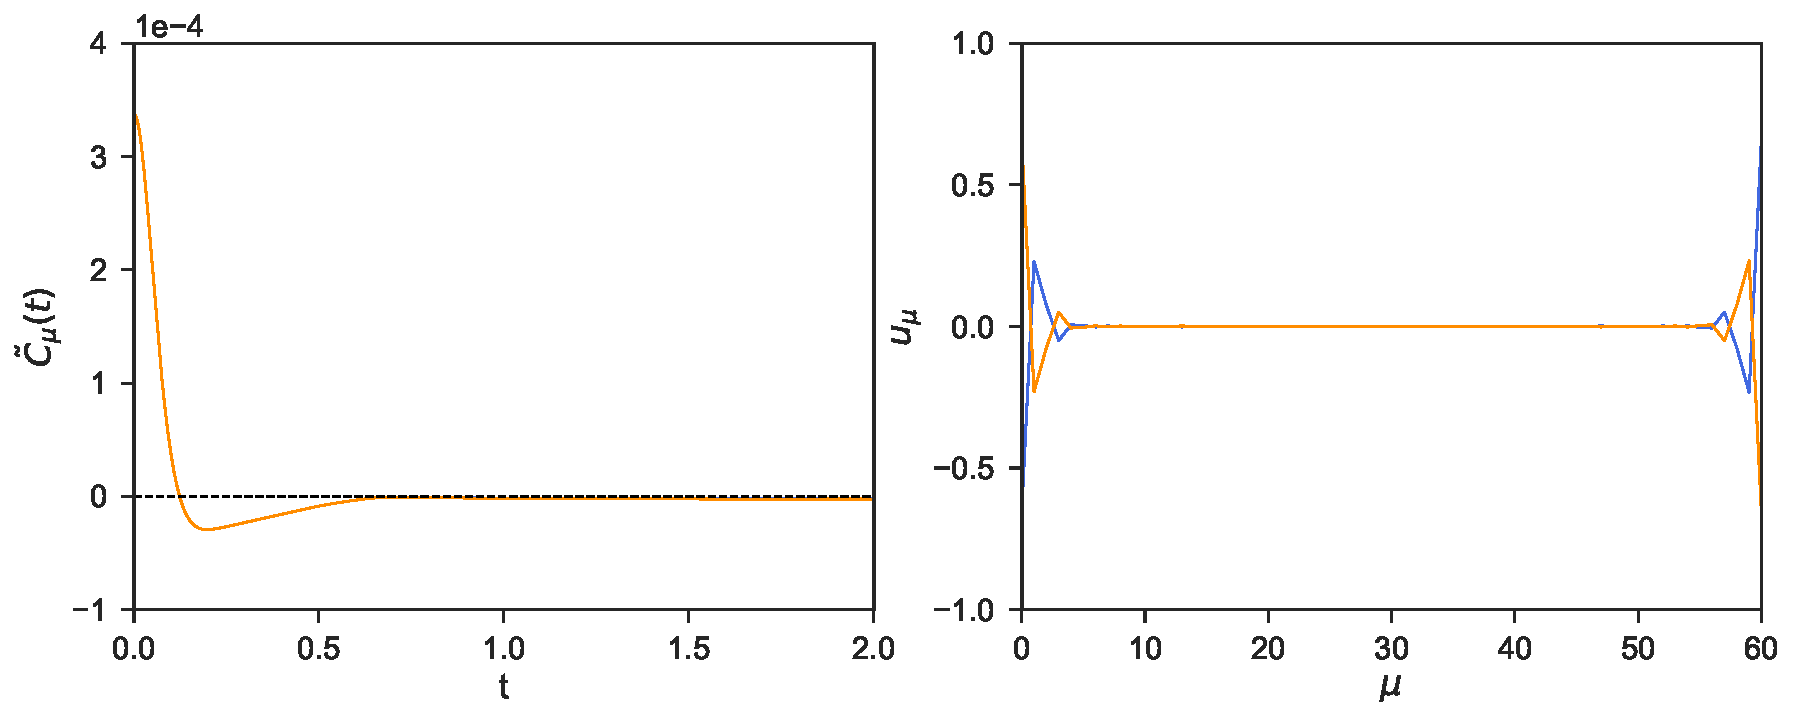
\includegraphics[width=\linewidth]{EigenvaluesVectors-WALLS-66nodes}
\caption[Eigenvalues and eigenvectors near the walls for 66 nodes.]{The eigenvalues $\tilde{C}_{\mu}(t)$ of the correlation matrix $C(t)$ for $\mu=59,60$ which are identical and superimpose (left) and the corresponding eigenvectors $u_{\mu}$ in blue and orange, respectively (right).}
\label{fig:EigenvaluesVectors-WALLS-66nodes}
\end{figure}

The fact  that there are  eigenvalues that decay in  a non-exponential
way indicates  that the dynamics  is non-Markovian, at least  near the
walls. The non-Markovian effects could  be small, however, as only one
eigenvalue  is clearly  non-exponential.  In  order to  appreciate the
actual effect  of this  non-Markovian contribution to  the correlation
matrix in real space, we define the relaxation matrix in Fourier space
as   $\tilde{\Lambda}^*=\tilde{\Lambda}(\tau)$  for   $\tau=0.2$.   As
appreciated in Fig.   \ref{fig:LambdatRec-WALLS-66nodes}, this time
$\tau$ seems to  be a compromise for the minimum  time at which almost
all the elements $\tilde{\Lambda}_\mu(t)$ have reached the plateau and
yet the statistical errors due to  the inverse of the eigenvalues have
not exploded.   From $\tilde{\Lambda}^*$  we construct  the relaxation
matrix $\Lambda^*$ in  real space and, from  equation  (\ref{Cpredict}), we
obtain the prediction $C^{\rm  predict}(t)$ of the correlation matrix.
\begin{figure}[h!]
  \centering
%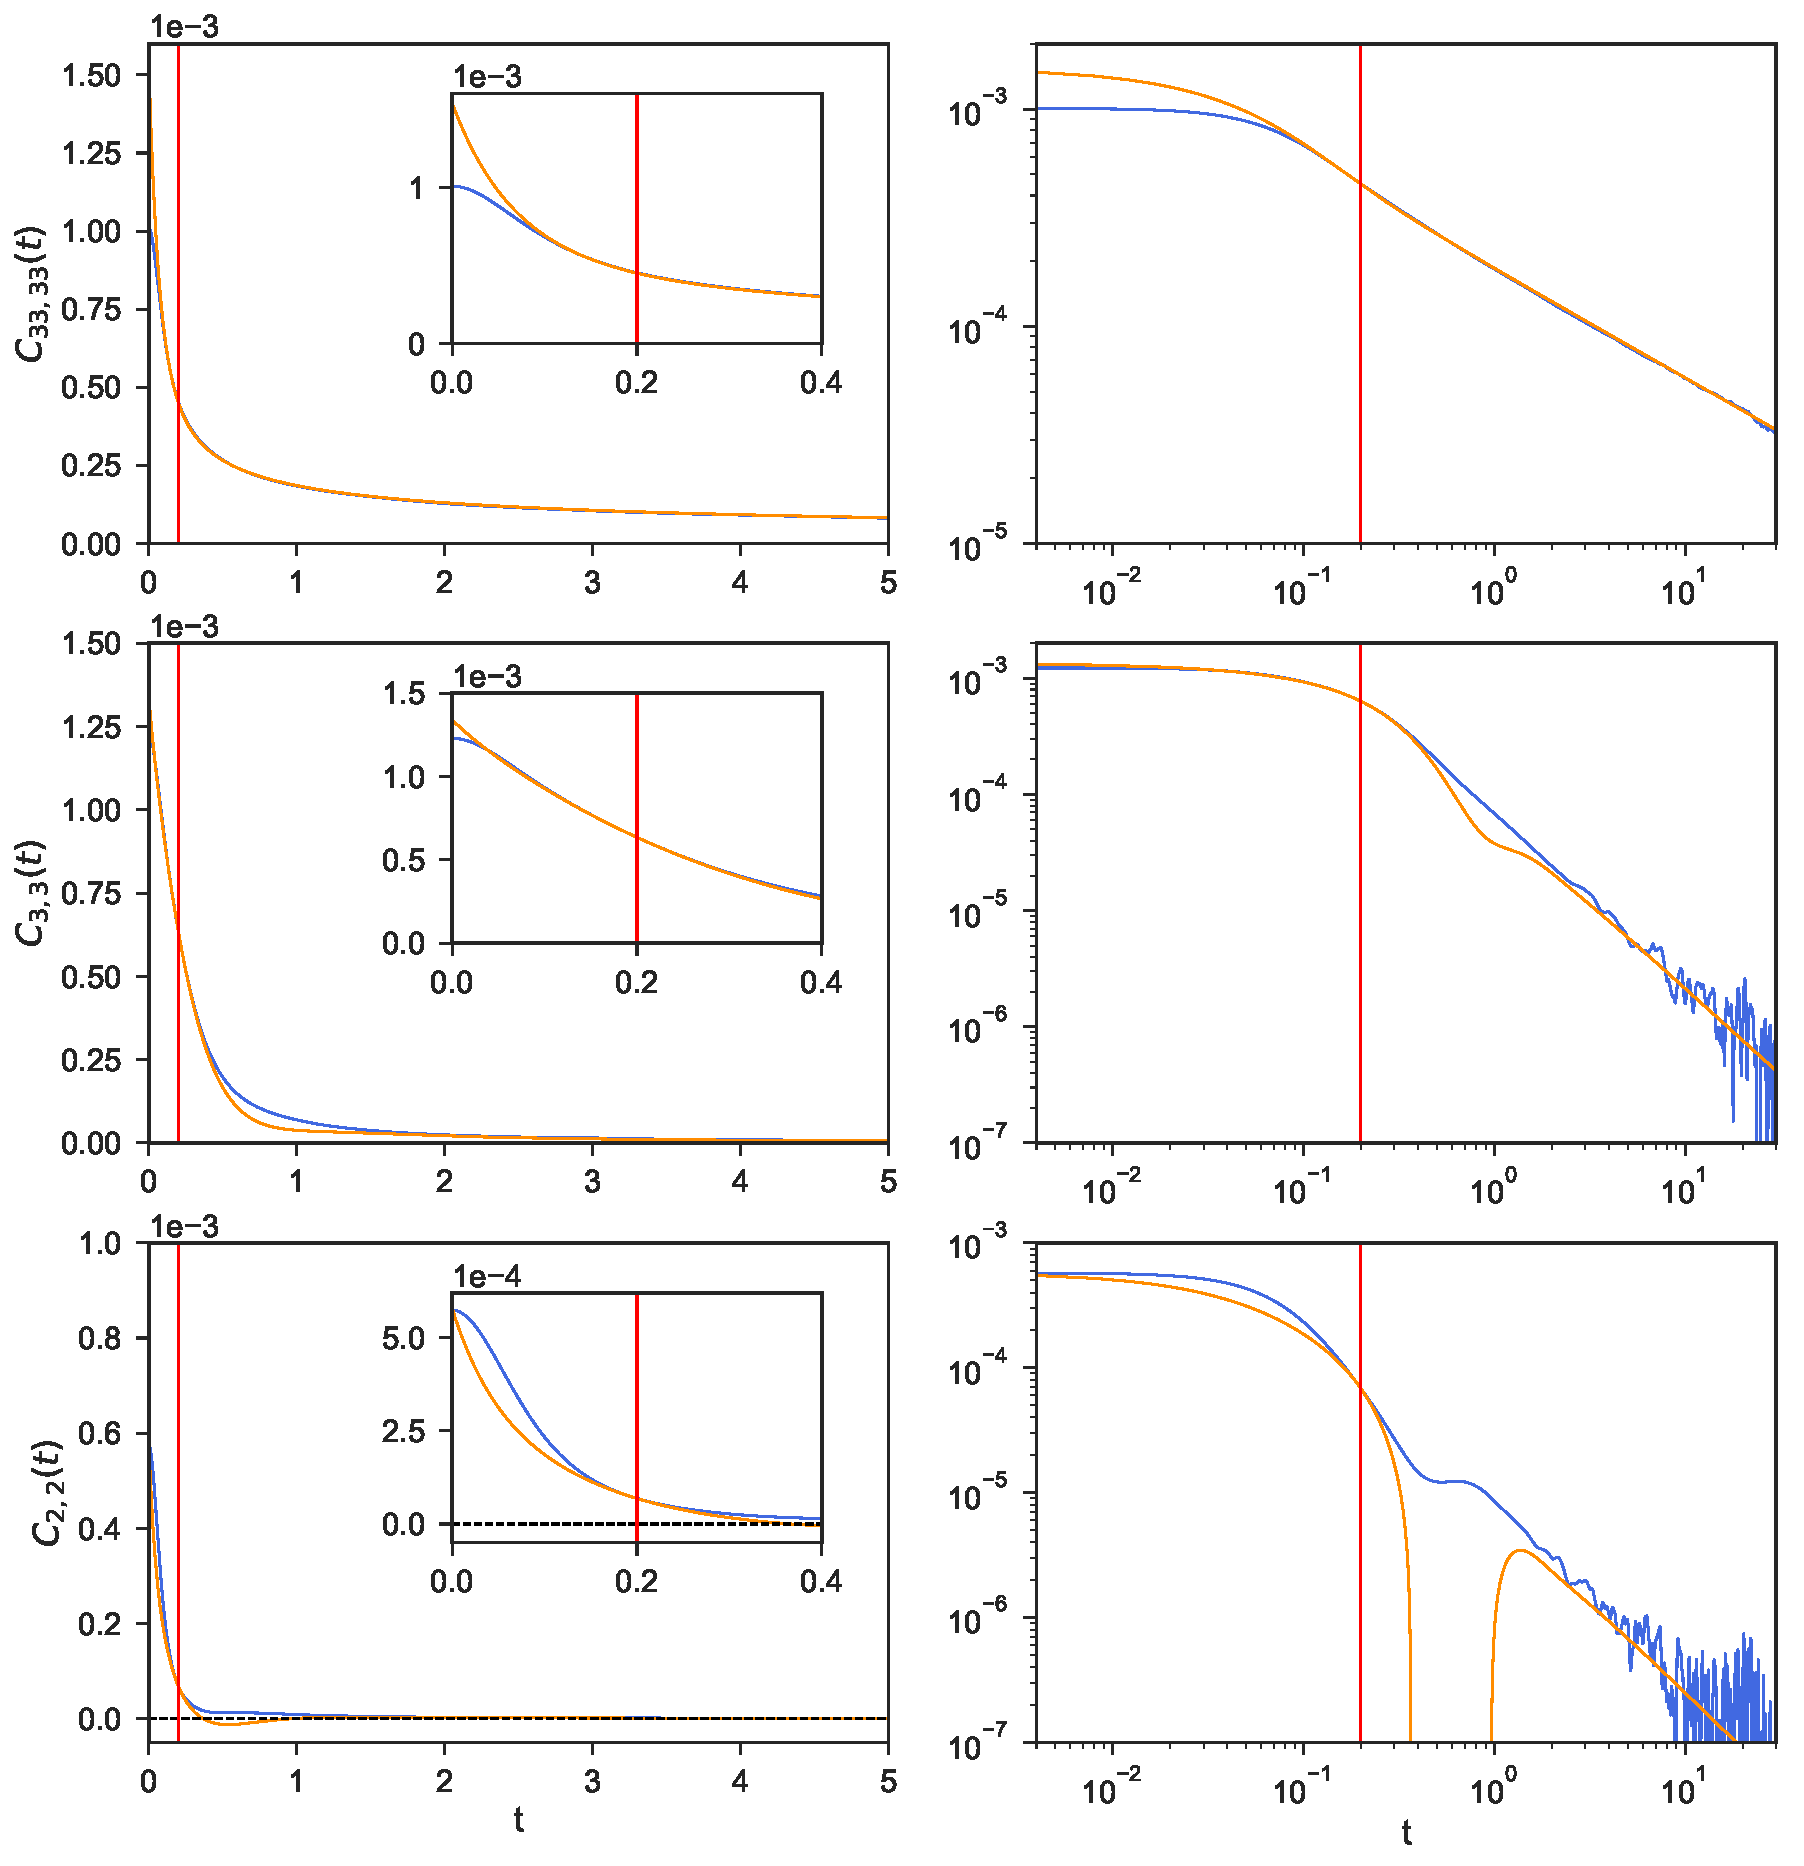
\includegraphics[scale=0.41]{Predictions-WALLS-66nodes}
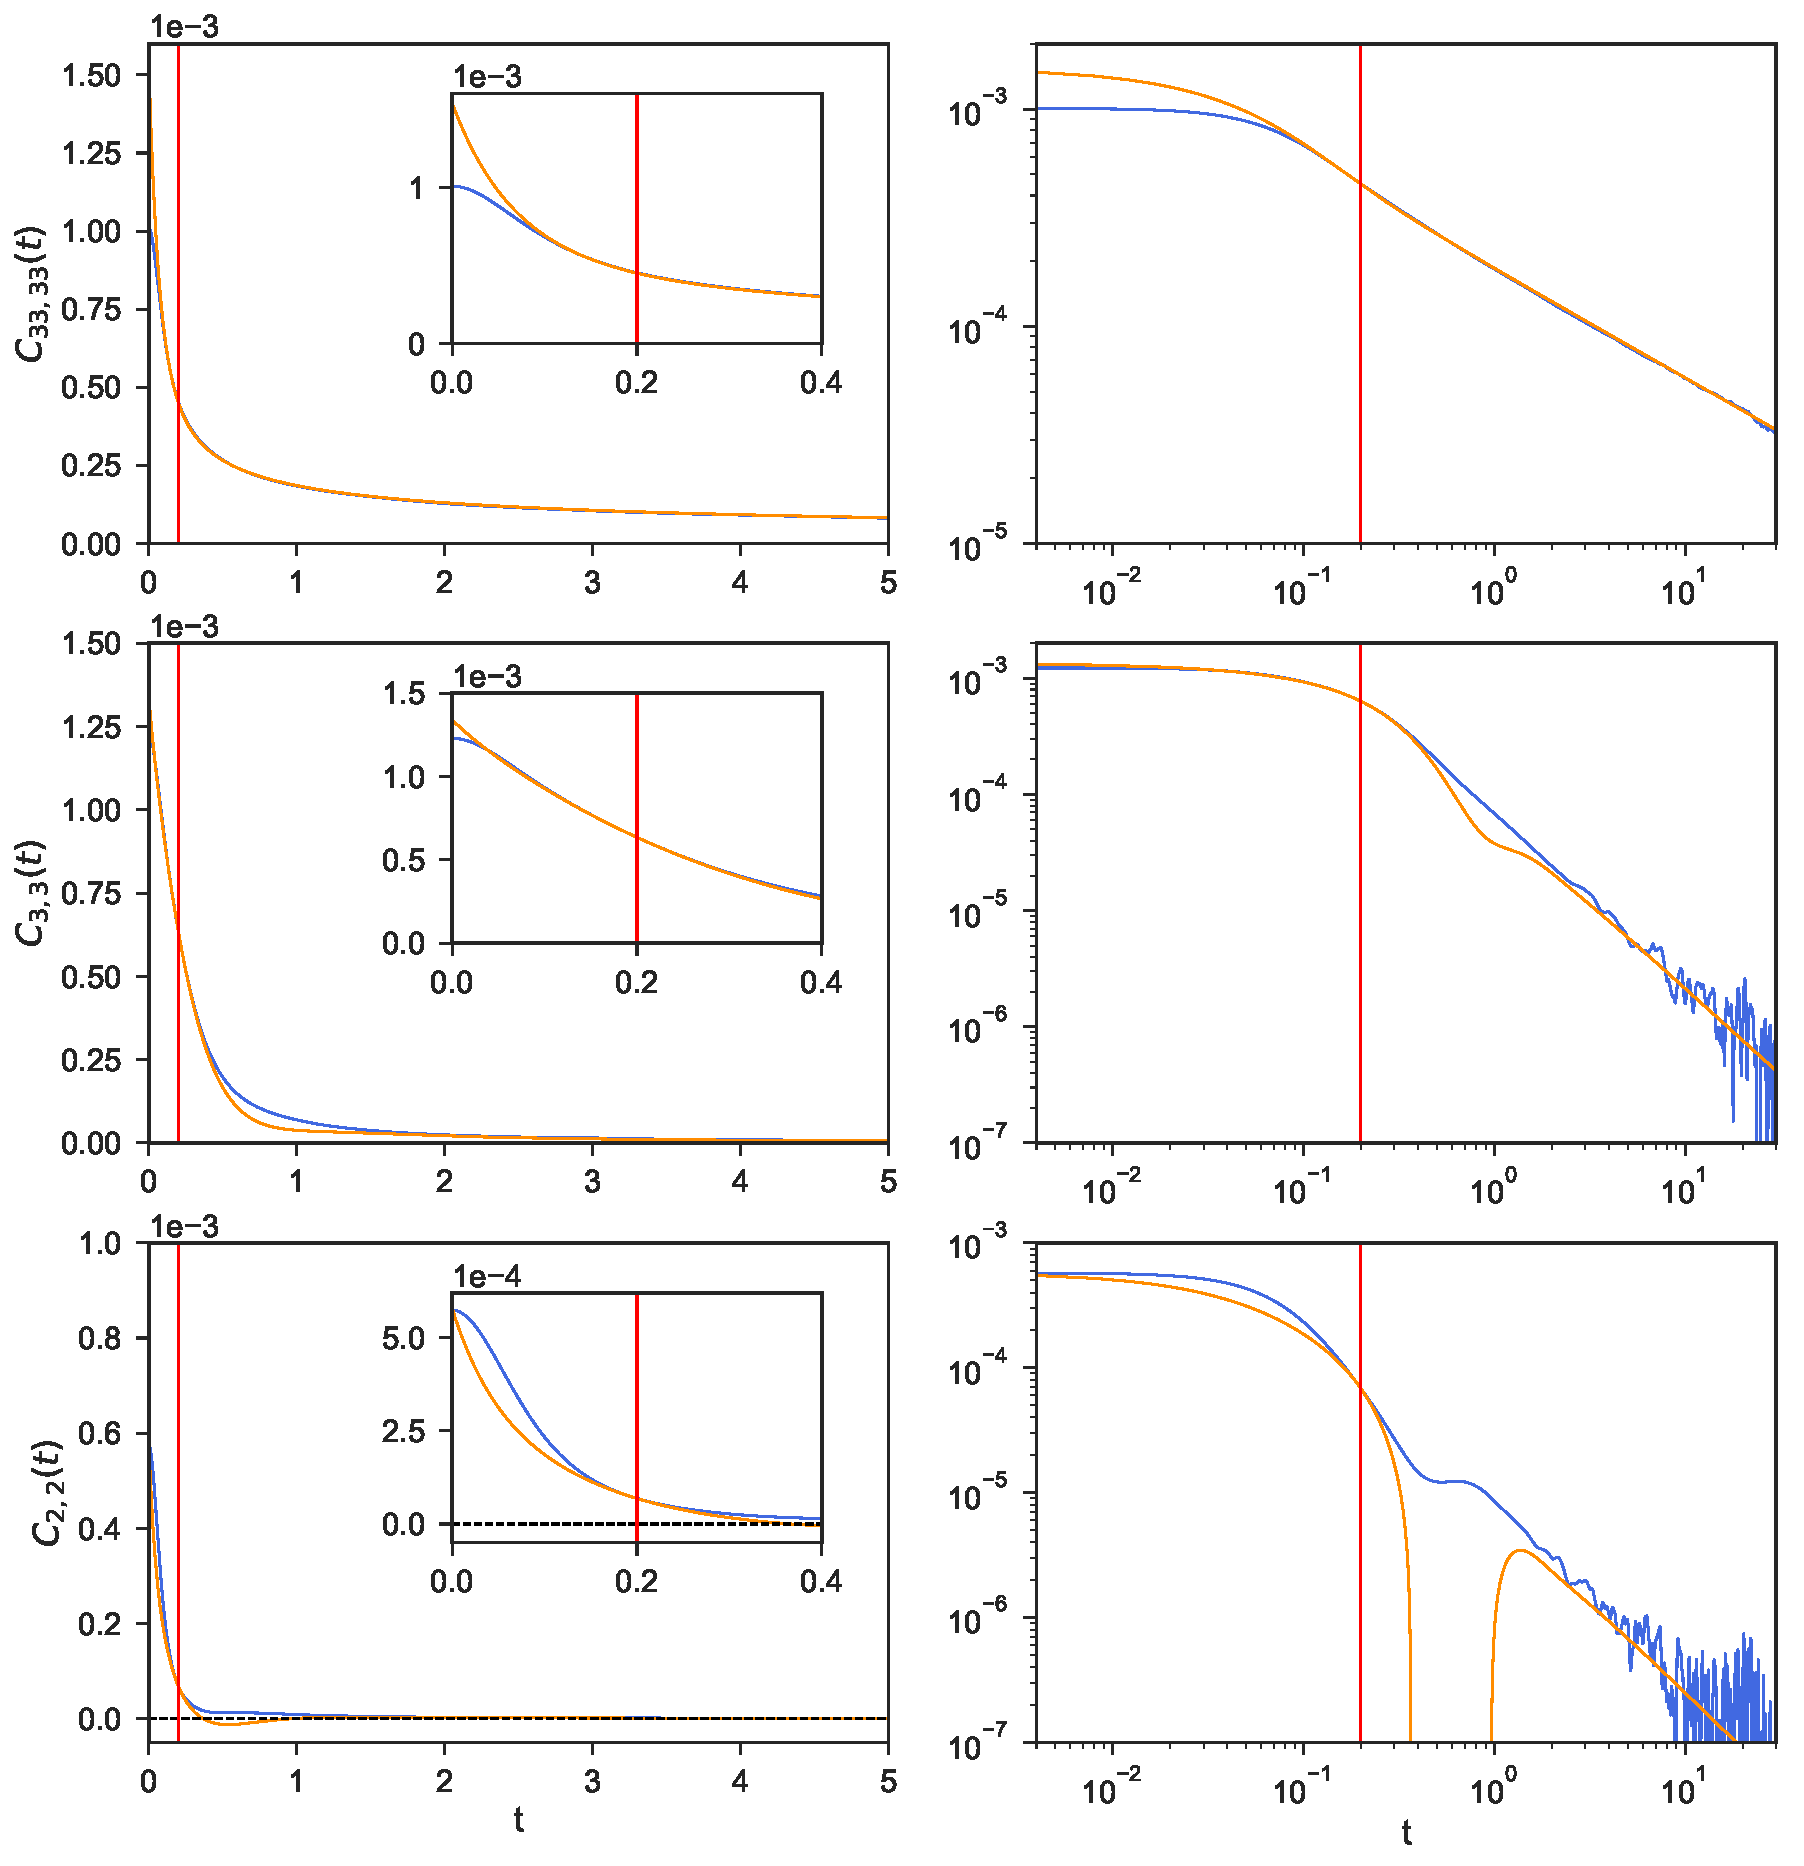
\includegraphics[width=\linewidth]{Predictions-WALLS-66nodes}
\caption[Predicted autocorrelations of $C(t)$ for 66 nodes.]{The predicted (orange) and the measured (blue) values of the autocorrelation $C_{\mu\mu}(t)$ at different values of $\mu$ (top $\mu=33$, middle $\mu=3$ and bottom $\mu=2$). The predicted and measured correlations coincide by construction at $t=\tau=0.2$, where the vertical red line is. The inset shows a zoom at short times. The right panel is the same in logscale, where the correlations extends up to time $t=30$.}
\label{fig:Predictions-WALLS-66nodes}
\end{figure}
We plot in Fig. \ref{fig:Predictions-WALLS-66nodes} the  comparison of the measured and the
predicted correlation matrix  for particular elements $C_{\mu\mu}(t)$
of the matrix  along the diagonal.  In particular,  we choose $\mu=33$
which is in the middle of the  channel and $\mu=2,3$ which are the two
bins closer to the walls that have already fluid in it (bins $\mu=0,1$
do not contain  fluid particles due to the presence  of the wall).  In
the  top  panel  of  Fig.   \ref{fig:Predictions-WALLS-66nodes} are  the  results  for  the
autocorrelation in the middle of  the channel. The inset is a zoom at short times. The right plot, in logscale,
has  a support  up  to  $t=30$. The  agreement  between predicted  and
measured correlations is excellent in  the middle of the channel.  The
middle  and  bottom  panels  in Fig.   \ref{fig:Predictions-WALLS-66nodes}  describing  the
comparison   near   the   solid   wall,   however,   show   noticeable
discrepancies.   Very close  to  the wall,  for  $\mu=2$ the  measured
correlation displays  a bump,  better noticed  in the  logscale plot,
that  probably  reflects  the   ``bounce-back''  contribution  of  the
eigenvalues  $\mu=59,60$ in  the correlation  matrix (\ref{spectral}).
The  measured  autocorrelation  remains positive,  though,  while  the
predicted correlation  becomes negative.  Therefore, we  conclude that
the measured relaxation  matrix $\Lambda^*$ does not  allow to predict
through (\ref{InFull-C})  the correct  momentum correlations  near the
wall.   This is  clear sign  that the  dynamics near  the wall  is not
Markovian.


\subsection{Thick bins with $\Delta z = 2\sigma$}
In  order to  assess the  effect  of the  bin width  on the  Markovian
character of the  dynamics of the discrete momentum  variable, we have
conducted simulations  of the  same system but  with 33  nodal planes,
giving bins  of a  size $\Delta  z=\sigma$, and  with 17  nodal planes
giving a  bin width of  $\Delta z=2\sigma$.  The phenomenology  for 33
nodes  is very  similar to  the one  for 66  nodes.  
We still observe negative eigenvalues and non-Markovian behaviour, although the effects are not so pronounced as for 66 nodes.  For this reason, we do not present the results for 33 nodes and present only the results for 17 nodes. 
\begin{figure}[h!]
  \centering
  %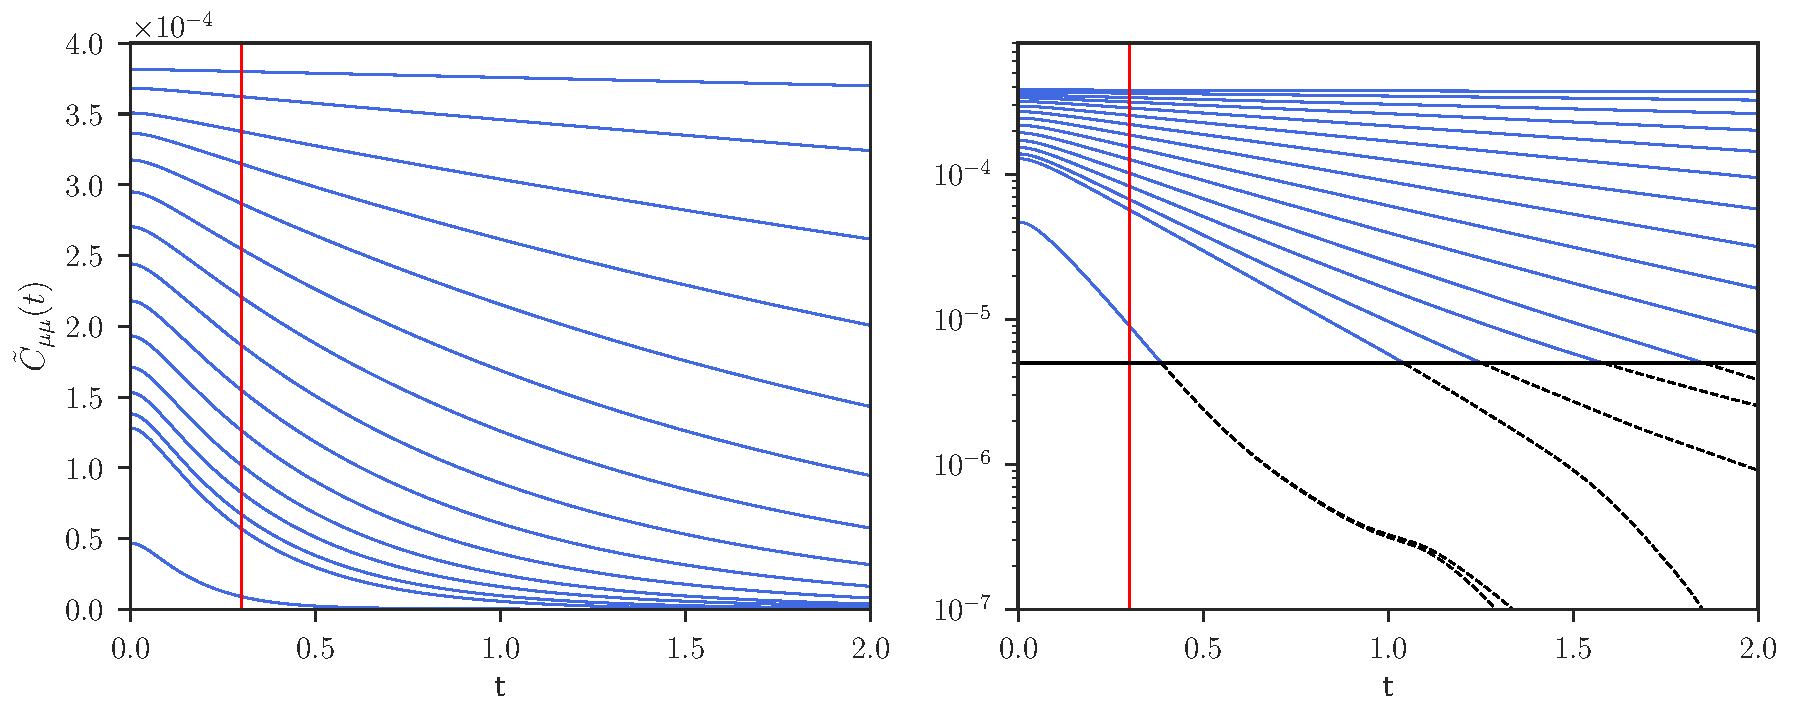
\includegraphics[scale=0.41]{CtRec-WALLS-17nodes-exp}
  \includegraphics[width=\linewidth]{CtRec-WALLS-17nodes-exp}
  \caption[Evolution of different eigenvalues $\tilde{C}_{\mu\nu}(t)$ for confined fluid - 17 nodes.]{
  The  evolution of  the different
  eigenvalues  $\tilde{C}_{\mu\mu}(t)$ of  the  correlation matrix  of
  momentum  as  a  function  of   time  in  a  lin-lin  plot  (left)
  and   log-lin   plot
  (right). Also  plotted are  a vertical line  at $t=\tau=0.3$  and a
  horizontal  line  at  the   value  $5\times10^{-6}$,  signaling  the
  threshold below which statistical errors give spurious results. }
\label{fig:CtRec-WALLS-17nodes-exp}
\end{figure}


\begin{figure}[h!]
  \centering
\includegraphics[scale=0.41]{LambdatRec-WALLS-17nodes}
\caption[Diagonal elements  $\tilde{\Lambda}_{\mu\mu}(t)$ of $\Lambda(t)$ in the reciprocal space - 17nodes.]{The  diagonal elements  $\tilde{\Lambda}_{\mu\mu}(t)$ of  the
  $\Lambda(t)$ in the reciprocal space defined in (\ref{LambdatRec}), as a
  function of $t$.}
\label{fig:LambdatRec-WALLS-17nodes}
\end{figure}

In  Fig.
\ref{fig:CtRec-WALLS-17nodes-exp}   (left   panel)   the   time   dependent   eigenvalues
$\tilde{C}_{\mu}(t)$  of  the  $17\times 17$  correlation  matrix  are
plotted as a function of time.  In the right panel, the logscale plot
shows a fairly linear decay, signaling exponential behaviour.  This is
more  clearly   seen  in   Fig. \ref{fig:LambdatRec-WALLS-17nodes},  where   the  function
$\tilde{\Lambda}_\mu(t)$  defined  in  (\ref{LambdatRec})  displays  a
plateau.  
\begin{figure}[h!]
  \centering
  \includegraphics[scale=0.41]{Eigenvectors-WALLS-17nodes}
    \caption[The igenvectors correspondings to the two largest eigenvalues of $\Lambda(t)$ for bins with $\Delta z=2\sigma$]{
        The eigenvectors correspondings to the two largest eigenvalues of $\Lambda(t)$}
\label{Fig.WallEigenvectors2}
\end{figure}
Note that  two eigenvalues are  clearly separated
from the rest.   These eigenvalues correspond to  the two eigenvectors
shown in  Fig. \ref{Fig.WallEigenvectors2} that clearly  correspond to
the  dynamics  near  the   walls.  
It is apparent  that the friction with the walls  has a strong damping
effect on  the fluid  near the wall.   From Fig. \ref{fig:LambdatRec-WALLS-17nodes} we
select the plateau  time $\tau=0.3$. This time is larger  than the one
selected for thinner bins because now the statistical errors are not so
pronounced.  We  measure  the  relaxation matrix  $\Lambda^*$  as  the
Fourier       transform       of       the       diagonal       matrix
$\tilde{\Lambda}_{\mu}^*(\tau)$.  In  this way,  we can  now construct
the prediction  (\ref{Cpredict}) for the correlation  matrix $C(t)$ in
real  space.    We  plot  in  Fig.    \ref{fig:Predictions-WALLS-17nodes}  some  selected
autocorrelations corresponding  to bins $\mu=7$  in the middle  of the
channel,  $\mu=4$ which  is  a  quarter distance  from  the wall,  and
$\mu=1$  the  first   bin  with  fluid  (bin  $\mu=0$   has  no  fluid
contribution).   We   observe  an  excellent  agreement   between  the
predicted and measured correlations.  This agreement is also very good
for the  cross-correlations, as shown in  Fig. \ref{fig:PredictionsCross-WALLS-17nodes}. Note
that the  cross-correlation $C_{8,7}(t)$ is non-zero  at $t=0$ because
the momentum at a  given node is defined in terms  of a finite element
basis  function.  For  neighbouring  nodes, the  finite element  basis
overlap  and this  gives  rise  to the  non-zero  value  of the  cross
correlation.  On  the other  hand, for nodes  separated by  two units,
where the finite elements no  longer overlap, the cross correlation at
$t=0$ vanishes, as it is clear for $C_{3,5}(t)$.

\newpage
\begin{figure}[h!]
  \centering
%\includegraphics[scale=0.41]{Predictions-WALLS-17nodes}
\includegraphics[width=\linewidth]{Predictions-WALLS-17nodes}
\caption[Predicted autocorrelations of $C(t)$ for 17 nodes.] {Autocorrelations $C_{\mu\mu}(t)$  for different  bins $\mu=1$
  (bottom),  $\mu=4$  (middle),  and  $\mu=7$ (top).  The  right panel  is  in 
  logscale with a support up to $t=30$. The red line is plot at $t=0.3$}
\label{fig:Predictions-WALLS-17nodes}
\end{figure}

\newpage
\begin{figure}[h!]
  \centering
%\includegraphics[scale=0.41]{PredictionsCross-WALLS-17nodes}
\includegraphics[width=\linewidth]{PredictionsCross-WALLS-17nodes}
\caption[Predicted crosscorrelations of $C(t)$ for 17 nodes.]{The crosscorrelations between nodes $\mu=3,\nu=5$ (bottom) and  $\mu=8,\nu=7$ (top). The right panel is in logscale, and the red line is plot at $t=0.3$.}
\label{fig:PredictionsCross-WALLS-17nodes}
\end{figure}

\section{Summary}
In this chapter we have considered  the discrete hydrodynamics of  a LJ
fluid  confined  between   two  rigid  parallel  walls   of  fixed  LJ
particles. We  measure the correlation  matrix $C(t)$ of  component of
the discrete momentum density which is  parallel to the walls.  According
to  Mori theory,  under the  Markovian approximation  this correlation
should decay  in a  matrix exponential form  with a  relaxation matrix
$\Lambda^*$ that  can be  obtained from the  plateau region  where the
decay  of  $C(t)$  is  exponential.  By  looking  at  the  eigenvalues
$\tilde{C}_\mu(t)$  of the  correlation  matrix,  the Markov  property
translates into an  exponential decay of all the  eigenvalues. We have
observed that  for bins  smaller than  molecular dimensions  $\Delta z
\leq  \sigma$,  where  $\sigma$  is  the  LJ  diameter,  some  of  the
eigenvalues do  not decay  as exponential  and become  negative.  Even
though we can estimate a relaxation matrix from the plateau that gives
good predictions away  from the wall, the correlations  near the walls
are poorly described by the Markovian theory.

When we  increase the  size of  the bins, up  to $\Delta  z=2\sigma$, a
Markovian theory gives excellent results, where all the eigenvalues of
the   correlation  function   decay   exponentially,  a   well-defined
relaxation  matrix  $\Lambda^*$ can  be  measured,  and the  resulting
predictions  with  this  relaxation  matrix reproduce  very  well  the
measured correlation matrix.

The present chapter follows the  methodology of Chapter \ref{Chap:PBC}  where we
have  discussed  the  correlation  matrix  of  the  discrete  momentum
parallel to  the bins in  an \textit{unconfined} system  with periodic
boundary  conditions.  We  have  observed there  that the  correlation
matrix for the discrete momentum defined  in thin bins of size $\Delta
z= 0.5\sigma$ behaves in a Markovian way. Of course, this behaviour is
observed  only beyond  certain time  $\tau$, as  observed also  in the
present chapter.  It is clear that the breaking of the Markov assumption
for thin bins is due to the presence of the walls, which is consistent
with  the   observation  that  the  eigenvectors   of  the  non-Markov
eigenvalues are different  from zero only near the  walls. The physics
behind this non-Markov  behaviour for thin bins is  not entirely clear
but  we note  that for  thin bins,  we are  resolving scales  that are
comparable   to   the   ``roughness''    of   the   lattice   of   the
walls. \Note{Duda sobre lo siguiente}Therefore, it is plausible that the bump in the autocorrelation
of the  bin close  to the lattice  shown in the  bottom panel  of Fig.
\ref{fig:Predictions-WALLS-66nodes} is  due to a  ``caging effect'' of the  fluid particles 
due to the lattice. Such a caging would be undetectable for much wider
bins, as it appears to be the case.

In  the  present  chapter,  we  have  only  discussed  the  dynamics  of
transverse momentum.   With the same  methodology, we can  discuss the
coupled  dynamics of  the  density  and the  normal  component of  the
momentum.   It is  not yet  clear to  us whether  the highly  resolved
hydrodynamics near  the wall, that  reproduce the density  layering as
shown in  Fig.  \ref{fig:DensityProfile-WALLS} is  Markovian or  not. In any  case, we
expect that the study of perpendicular sound waves confined in between
parallel walls deserves further study.

\begin{figure}[h!]
  \centering
\includegraphics[scale=0.41]{DensityProfile-WALLS}
\caption[Fluid density profile for 66 and 17 nodes.]{The equilibrium average discrete density for thin bins (blue) and thick bins (orange). The thick bins do not capture the layering of the density field.}
\label{fig:DensityProfile-WALLS}
\end{figure}

The  fact that  hydrodynamics near  walls is  non-Markovian at  highly
resolved  scales  has a  number  of  implications. For example, in Chapter \ref{Chap:Theory} the delta function introduced in the hydrodynamic fields can not be a Dirac $\delta$ functions. 
The continuum theory  described in Chapter \ref{Chap:Theory} can  only make
sense if the hydrodynamic fields are  defined not with the Dirac $\delta$
function, but  rather with  coarse delta  functions with  an intrinsic
length  scale  larger than  molecular  dimensions  as, for  example  a
normalized Gaussian  of width  $\sigma$.  As  a consequence,  the free
energy functional  that emerges from  such a coarsely  defined density
field  is not  directly  given by  the usual  free  energy density  in
equationilibrium  Density Functional  Theory, which  is, in  fact, the  one
particle distribution function.  In fact,  a local model for the free energy 
is expected for  the former. The resulting free  energy functional for
coarsely  defined density  cannot  resolve the  density layering  near
walls.   It is  obvious now  that in  order to  describe the  resolved
dynamics of the density layering  near a wall requires a non-Markovian
theory  or,   alternatively,  a   Markovian  theory   with  additional
non-hydrodynamic variables.  Perhaps the  stress tensor is a candidate
to capture the apparent viscoelasticity of the density layering.

Note   that   it    only   make   sense   to    speak   of   transport
\textit{coefficients} (or matrices of) in theories that are Markovian,
otherwise  one  needs   transport  \textit{memory  kernels}.   Another
implication of  non-Markovianity of  highly resolved  hydrodynamics is
that in order  to speak about the the  nonlocal friction coefficients
as the ones  described by Camargo et al. in \cite{CamargoBC2018} one  has to ensure
that the  bins are larger  than the  molecular size. In  the following chapter we will  measure  the nonlocal  viscosity and  nonlocal
friction matrices that are buried in the relaxation matrix $\Lambda^*$
and  that  have  not  been  considered in  this chapter.  These
transport matrices enter  into the microscopic definition  of the slip
length.


%-----------------------------------------------------------------
%CHAPTER 6
%-----------------------------------------------------------------
\chapter{The slip boundary condition}
\label{Chap:Slip}
\epigraph{\textit{It is remarkable how long men will believe in the bottomlessness of a pond without taking the trouble to sound it.}}{Walden \\ HENRY DAVID THOREAU}
\markboth{The slip boundary condition from MD simulations}{}

\section{Introduction}

In this chapter, we compute explicitly the viscosity and friction kernels that appear in the discrete hydrodynamic theory presented in Chapter \ref{Chap:Planar} for shear flows in between confining paralle solid walls.  
We show  that  the  usual Green-Kubo  formulas  suffer
dramatically  from the  plateau problem  and  cannot be  used for  the
unambiguous  determination of  transport coefficients.   This includes
the solid-fluid friction coefficient which,  as shown in Ref. \cite{CamargoBC2018},
is  equivalent  to   the  expression  given  by   Bocquet  and  Barrat
\cite{Bocquet1994}.  We  use the corrected Green-Kubo  expressions, as
formulated in  Chapter \ref{Chap:PBC}, in  order to determine  unambiguosly the
transport kernels (which are matrices for the nonlocal viscosity and
nonlocal frictions).  With  these transport matrices, we  are able to
predict correctly the evolution  of the \textit{correlation} matrix of
the  discrete  hydrodynamic  variables.  We  also  validate  Onsager's
hypothesis  by  predicting,  with  the same  transport  matrices,  the
evolution of the \textit{average} of  the discrete momentum field.  By
looking at the equations for the averages of hydrodynamic variables we
may reproduce the pillbox argument of Ref.  \cite{CamargoBC2018} and re-derive the
Navier slip boundary condition.  This provides an explicit microscopic
expression for the  slip length that involves  the corrected transport
kernels.  The  present formulation with corrected  Green-Kubo formulas
predicts  the  boundary  conditions  that should  be  imposed  on  the
evolution equations for the average hydrodynamic variables. We observe
in nonequilibrium  MD simulations  that the  plug flow  considered in
this chapter violates the Navier slip boundary condition at short times,
while it is very  well  satisfied at  later stages  of  the flow.   This
violation is due to the unbalance between the solid friction and shear
force,  which is  at the  base of  the derivation  of the  Navier slip
boundary  condition $\delta\frac{\partial v}{\delta z}=v_{{\rm slip}}$ derived in the Introduction.   Finally, we  also show  that the
corrected Green-Kubo  transport kernels do describe  intrinsic surface
properties by  observing that  the slip length  is independent  on the
channel width.

\section{The CG variables}
\label{Sec:CGSlip}
Although some of the expressions and mathematical derivations in this section and the following one  have been obtained in the previous chapters, it is convenient to include them in order to follow-up this chapter.

We consider a monoatomic fluid  confined in between two parallel solid
walls in the  $x,y$ directions while the normal axis  $z$ to the
walls is divided in $N_{\rm bin}$  bins separated by nodal planes.  In Chapter \ref{Chap:Planar}
we  have obtained a set of evolution  equations for the
discrete  mass and  momentum densities  of a  fluid moving  in between
parallel  walls and  under  the  assumption that  the  flow is  itself
traslationally invariant  along the  directions parallel to  the solid
walls.  When  the flow field  is parallel to  the walls like  in shear
flows (excluding the case of sound  waves normal to the walls), the CG
variable is the  parallel component ${\bf g}^x_\mu$  of the discrete
momentum field defined on each nodal plane $\mu=0,\cdots,N_{\rm bin-1}$.
The microscopic definition of the discrete momentum is
\begin{align}
  \hat{\bf g}_\mu=\sum_i^N{\bf p}_i\delta_\mu({\bf r}_i),
\label{hatg}
\end{align}
where ${\bf r}_i,{\bf p}_i$ are the  position and momentum of the i-th
atom and  $\delta_\mu({\bf r})$  is proportional  to a  finite element
basis  function, as  described in  detail in  Chapter \ref{Chap:Planar}.
We will
collect   the    CG   variable    (\ref{hatg})   into    an   $N_{\rm
  bin}$-dimensional   column  vector   $\hat{g}$   that  contains   as
components  the parallel  component  of the  momentum  density of  bin
$\mu$,  this  is $\hat{g}^T=(\hat{\bf g}^x_1,\cdots,\hat{\bf g}^x_{\rm bin})$,  where  the
superscript $T$ denotes the transpose.



\subsection{Time derivatives}
As shown  in Chapter \ref{Chap:Planar}
the momentum  density changes due  to the
discrete force density $ \hat{\bf F}_\mu$ that the solid exerts on the
fluid at node $\mu$ and to  the discrete gradient of the stress tensor
$\hat{ \boldsymbol{\sigma}}_{\mu}$ of bin $\mu$, this is
\begin{align}
  i{\cal L}\hat{\bf g}_\mu(z) &=\hat{\bf F}_\mu(z)-\frac{\hat{\boldsymbol{\sigma}}_\mu(z)-\hat{\boldsymbol{\sigma}}_{\mu-1}(z)}{\Delta z}\esc{\bf e}_z,
\label{equationivalenceSlipCH}
\end{align}
where the force density and the stress tensor are given, respectively, by the equations \ref{Fbin} and \ref{sbin}.

%we have the
%following microscopic definitions
%\begin{align}
%  \hat{\bf F}_\mu &= \sum_{ij'}^{NN'}\hat{\bf F}_{ij'}\delta_\mu({\bf r}_i)
%\label{Fbin}\\
% \hat{ \boldsymbol{\sigma}}_{\mu}
%&=
%\frac{1}{{\cal V}_\mu} \left[\sum_i{\bf p}_i{\bf v}_i\chi_\mu({\bf r}_i)
%+\frac{1}{2}\sum^{N}_{ij}{\bf r}_{ij}\hat{\bf F}_{ij}z_\mu(i,j)\right]
%\label{sbin}
%\end{align}
The  stress   tensor  $\hat{\boldsymbol{\sigma}}_\mu$  of   bin  $\mu$
contains  only   coordinates  and   velocities  of   fluid  particles
$i=1,\cdots,N$,  while the  force  density $\hat{\bf  F}_\mu$ of  node
$\mu$ contains  the force  $\hat{\bf F}_{ij'}$  that a  wall particle
$j'=1,\cdots, N'$  exerts on a  liquid particle $i$.  
%Recall that the geometrical factor $z_\mu(i,j)$ is
%the fraction of the length of the segment joining particles $i,j$ that
%happens  to be  inside the  bin.  
For  the parallel  component of  the
momentum, equation (\ref{equationivalenceSlipCH}) becomes
\begin{align}
  i{\cal L}\hat{g}_\mu(z) &=\hat{F}_\mu(z)-\frac{\hat{\sigma}_\mu(z)-\hat{\sigma}_{\mu-1}(z)}{\Delta z},
\label{equationivalence2}
\end{align}
where  we  have  collected  into  vectors  the  forces  and  stresses,
$\hat{F}_\mu=\hat{\bf                   F}_\mu^x$                  and
$\hat{\sigma}_\mu=\hat{\boldsymbol{\sigma}}^{xz}_\mu$.   We may  write
equation (\ref{equationivalence2}) in matrix form as
\begin{align}
  i{\cal L}\hat{g}&= \hat{F}+ F^T\esc\hat{\sigma},
\label{iLgMat2}
\end{align}
where $\hat{F}$ and $\hat{\sigma}$ are $N_{\rm bin}$-dimensional column vectors and 
the matrix $ F$  is the bi-diagonal forward finite difference
operator introduced in equation \ref{Dforward}.
%\begin{align}
% {F}=\frac{1}{\Delta z}\left(
%    \begin{array}{rrrrr}
%-1&1&0&\cdots&0\\
%0&-1&1&\cdots&0\\
%\vdots      &&\ddots&&\vdots\\
%\\
%0&\cdots&0&-1&1 
%\\
%0&\cdots&0&0&-1 \end{array}
%\right)
%\label{Dforward}
%\end{align}

\subsection{Correlation matrices}
The equilibrium time-correlation matrix of the transverse momentum is denoted by
\begin{align}
  C(t) &=  \llangle \hat{g}(t) \hat{g}^T \rrangle
\end{align}
At time  $t=0$ the time-correlation matrix is the covariance matrix
\begin{align}
C(0)&=   \llangle \hat{g}\hat{g}^T\rrangle 
\label{cov}
\end{align}
We may  now use  the decomposition (\ref{iLgMat2})  in order  to relate
correlations of momenta, stresses, and  forces. First, write the time
derivative of the correlation matrix of the transverse momentum in the
following form
\begin{align}
\dot{C}(t)&=  -\int_0^t dt' \frac{d}{dt'}\llangle \hat{g}(t') i{\cal L}\hat{g}^T\rrangle
=-  \int_0^t dt' \llangle i{\cal L}\hat{g}(t') i{\cal L}\hat{g}^T\rrangle
\nonumber\\
&=-  k_BT M(t),
\label{dCMt}
\end{align}
where we have used Green-Kubo running integral (\ref{Mmunu}), i.e.
\begin{align}
M(t)&= \frac{1}{k_BT}\int_0^t dt'\langle i{\cal L}\hat{g}(t')i{\cal L} \hat{g}^T\rangle
\label{Mmunut}
\end{align}
 % and the matrix $C^{-1}(0)$ is proportional to the inverse of the covariance matrix
% \begin{align}
%  C^{-1}(0)&= k_BT C^{-1}(0)= M^\psi\esc\rho^{-1}
% \end{align}

By   substituting
(\ref{iLgMat2}) in the Green-Kubo integral (\ref{Mmunut}) we have
\begin{align}
{M}(t)&=F^T\esc{\eta}(t)\esc F+{G}(t)\esc F+F^T\esc{H}(t)+{\gamma}(t),
\label{MMatrix1}
\end{align}
where the  $N_{\rm bin}\times N_{\rm bin}$  matrices ${\eta}(t),{G}(t),{H}(t),{\gamma}(t)$
have as components the following Green-Kubo running integrals
\begin{align}
\eta_{\mu\nu}(t)
% &\equiv  \int \frac{d{\bf r}}{{\cal V}_\mu}
% \int \frac{d{\bf r}'}{{\cal V}_\nu}
% \chi_\mu({\bf r})
% \eta({\bf r},{\bf r}')\chi_\nu({\bf r})
% \nonumber\\
&=\frac{1}{k_BT}\int_0^t dt'
\left\langle \hat{\boldsymbol{\sigma}}^{xz}_{\mu}(t')\hat{\boldsymbol{\sigma}}^{xz}_{\nu}
\right\rangle
\nonumber\\
  G_{\mu\nu}(t)&=\frac{1}{k_BT}\int_0^t dt'
\left\langle\hat{\bf F}^x_\mu(t')
\hat{\boldsymbol{\sigma}}^{xz}_\nu
\right\rangle
%\nonumber\\
% &{\red \equiv \int \frac{d{\bf r}}{{\cal V}_\mu}\int \frac{d{\bf r}'}{{\cal V}_\nu}
% \psi_\mu({\bf r})G({\bf r},{\bf r}')
% \chi_\nu({\bf r}')}
\nonumber\\
H_{\mu\nu}(t)&=
\frac{1}{k_BT}\int_0^t dt'
\left\langle\hat{\boldsymbol{\sigma}}^{xz}_\mu(t')\hat{\bf F}^{x}_\nu\right\rangle
% {\red \equiv \int \frac{d{\bf r}}{{\cal V}_\mu}\int \frac{d{\bf r}'}{{\cal V}_\nu}
% \chi_\mu({\bf r})
% H({\bf r},{\bf r}')
% \psi_\nu({\bf r}')}
\nonumber\\
  \gamma_{\mu\nu}(t)
% \equiv \int \frac{d{\bf r}}{{\cal V}_\mu} \frac{d{\bf r}'}{{\cal V}_\nu}
% \psi_\mu({\bf r})\gamma({\bf r},{\bf r}')\psi_\nu({\bf r}')
% \nonumber\\
&=\frac{1}{k_BT}\int_0^t dt'
\left\langle 
\hat{\bf F}^{x}_\mu(t')
\hat{\bf F}^{x}_\nu\right\rangle
\label{GK}
\end{align}
We  have thus  expressed  the  matrix $M(t)$  in  terms of  Green-Kubo
formula    that   involve    the    nonlocal   transport    matrices
$\eta(t),G(t),H(t),\gamma(t)$.   The  matrix   $\eta_{\mu\nu}$  is   a
nonlocal      viscosity      kernel,     while      the      matrices
$G_{\mu\nu},H_{\mu\nu},\gamma_{\mu\nu}$ describe  the friction  of the
fluid with the walls.

% {\blue
% We may express also the Green-Kubo integral in the compact form
% \begin{align}
%   M(t)=F^T\esc\eta(t)\esc F+\Gamma(t)
% \end{align}
% where the matrix $\Gamma(t)$ contains the effects of the wall forces
% and it is given by the symmetric matrix
% \begin{align}
% \Gamma(t)&={G}(t)\esc F+F^T\esc{H}(t)+{\gamma}(t)  
% \end{align}
% }
Equations  (\ref{dCMt}) and (\ref{MMatrix1}) lead to the following mathematical identity
\begin{align}
\dot{C}(t)&=-k_BT\left[{F}^T\esc{\eta}(t)\esc{F}+{G}(t)\esc{F}+{F}^T\esc{H}(t)+{\gamma}(t)\right]
\label{CIdent}
\end{align}
This mathematical  identity relates correlations of  momenta with correlations of stresses
and forces. It is a useful identity  to check for errors in coding the
algorithms that  compute these quantities.  It also suggests  that the
Green-Kubo formulae  (\ref{GK}) must  decay to  zero because  the left
hand side of (\ref{CIdent}) certainly decays to zero.  In other words,
the Green-Kubo formulae (\ref{GK}) suffer from the plateau problem and
cannot  be  used  as  an   unambiguous  method  to  measure  transport
coefficients.


\section{The dynamics of the discrete transverse momentum}
\label{Sec:dyn}
Mori theory, as it was introduced in Chapter \ref{Chap:NESM}, allows one to obtain
exact closed equations for both, the  averages of the CG variables and
their  correlations.  The  exact  equations give  the  value of  these
quantities  in  terms  of  their  past history.   If  there  exists  a
separation of time  scales, the Markovian approximation  allows one to
approximate  the  exact  integro-differential  equations  with  simple
ordinary differential equations with no  memory (see equation (\ref{AproxCg})).  When we apply Mori's
theory with the Markovian approximation  to the particular CG variable
given by the transverse discrete  momentum $\hat{g}(z)$, we obtain the
dynamic  equation for  the  evolution of  its nonequilibrium  average
$g(t)$
\begin{align}
 \frac{d}{dt}g(t)&= -k_BT M^*\esc C^{-1}(0) \esc g(t), 
\label{InFull}
\end{align}
and the evolution equation for the equilibrium time correlation matrix
 \begin{align}
 \frac{d}{dt}C(t)&= -k_BT M^*\esc C^{-1}(0)C(t)
\label{InFull-C-2}
\end{align}
%where we have  redefined the matrix
%$M^*$ with a temperature prefactor $1/(k_BT)$ in order to make contact
%with usual  definitions later  on. 
Note  that the  transverse momentum
does not  have any reversible  contribution.  This is,  the reversible
matrix  
vanishes ($L=\llangle \hat{g}  i{\cal  L}\hat{g}\rrangle=0$) and  the
evolution of the transverse momentum is purely dissipative.

As  discussed  in Chapter \ref{Chap:PBC},
the  dissipative matrix  $M^*$  is
related to  the Green-Kubo  matrix $M(t)$ defined  in (\ref{MMatrix1})
through the \textit{corrected} Green-Kubo formula
\begin{align}
  M^*=M(\tau)\esc c^{-1}(\tau)
\label{Mstar}
\end{align}
%where the normalized correlation matrix is given by 
%(\ref{cnorm})
%\begin{align}
%  c(t)=C^{-1}(0)\esc C(t) 
%\end{align}
%which equals  the identity  matrix at  $t=0$.  
In  equation  (\ref{Mstar}),
$\tau$ is  a time where  the right hand  side reaches a  plateau. Note
that  the Green-Kubo  matrix $M(t)$  does  not display  a plateau  and
decays,  precisely, as  the  correlations themselves,  as observed  in
Chapter \ref{Chap:PBC}.  Therefore,  the  matrix  $M^*$  does  indeed  have  a
well-defined plateau for which the  value of $\tau$ is irrelevant once
the  plateau is  reached.  In  practice,  because the  inverse of  the
correlation matrix amplifies exponentially  any statistical error, the
value of $\tau$  should be chosen as the smallest  one that is already
in the plateau region.

By   using    (\ref{Mstar}) and (\ref{MMatrix1})   in   the   dynamics    of   correlations
(\ref{InFull-C-2}) we obtain
\begin{align}
  \dot{C}(t) =
-k_BT\left[{F}^T{\eta}(\tau)\esc{F}\esc  +{G}(\tau)\esc F+F^T\esc{H}(\tau)+{\gamma}(\tau)\right]
\esc C^{-1}(\tau) \esc C(t)
\label{CMarkov2}
\end{align}
Observe that the  use of the corrected starred  Green-Kubo expressions in
(\ref{InFull-C-2}) is  entirely equivalent  to use the  usual Green-Kubo
formula $M(\tau)$ but with a redefinition of the normalization of the
correlation,    from    $C^{-1}(0)$    to   $C^{-1}(\tau)$    as    in
(\ref{CMarkov2}).   Observe  also  that  for  $t=\tau$  the  dynamic
equation (\ref{CMarkov2}) becomes an identity, as  it complies with  the theorem
(\ref{CIdent}).   The   actual  value  of  $\tau$   is  irrelevant  in
(\ref{CMarkov2}) provided that  we are in the plateau  region of $M^*$
but,  as  mentioned, cannot  be  taken  too  large  in order  to  have
controlled statistical errors.

In  a similar  way, by  inserting (\ref{Mstar})  in (\ref{InFull})  we
obtain the following equation for the average of the discrete momentum
field
\begin{align}
   \frac{d}{dt}g(t)= -k_BT \left[{F}^T{\eta}(\tau)\esc{F}
+{G}(\tau)\esc{F}
+F^T\esc{H}(\tau)+{\gamma}(\tau)\right]
\esc C^{-1}(\tau)\esc  g(t) 
\label{evolg}
\end{align}
This matrix equation is best described in terms of the velocity field.
By following  the discussion  in Chapters \ref{Chap:Planar} and \ref{Chap:PBC}, we  define the  discrete
velocity field according to
\begin{align}
  {\bf v}_\mu&=\sum_{\nu}\rho_{\mu\nu}^{-1}{\bf g}_\nu,
\label{Vel}
\end{align}
where the mass density  matrix is defined as
\begin{align}
\rho_{\mu\nu}=\frac{C_{\mu\nu}(0)}{k_BT}  {\cal V}_\nu
\label{rhomunuAp}
\end{align}
Therefore,  we  may  introduce  the  vector  of  velocities
$v^T=(v_0,\cdots,v_{N_{\rm bin -1}})$ as
\begin{align}
v(t)&\equiv  k_BT{\cal V}^{-1}C^{-1}(0) \esc g(t) ,
\label{Vel2}
\end{align}
where the diagonal  matrix ${\cal V}$ contains the  volume elements of
each bin.  For bins of equal volume, the matrix ${\cal V}$ is just the
identity  matrix times  the volume  $L_xL_y\Delta  z$ of  a bin.   For
momentum profiles that  are smooth, the definition  (\ref{Vel}) of the
velocity  gives a  result that  is very  similar to  ${\bf v}_\mu={\bf
  g}_\mu/\rho_\mu$, where $\rho_\mu$ is the average density profile.


In terms of the velocity (\ref{Vel2}) the evolution equation (\ref{evolg}) is
\begin{align}
   \frac{d}{dt}g(t)= -\left[{F}^T{\eta}(\tau)\esc{F}
+{G}(\tau)\esc{F}
+F^T\esc{H}(\tau)+{\gamma}(\tau)\right]
\esc c^{-1}(\tau)\esc v(t)
\label{evolg2}
\end{align}

In this way, the transport equation (\ref{InFull}) becomes
\begin{align}
 \frac{d}{dt}g(t)&= - {\cal V}\esc M^*\esc v(t) 
\label{InFullVel}
\end{align}
that can be  expressed in the equivalent form
\begin{align}
   \frac{d}{dt}g(t)&=  - {\cal V}\esc M(\tau)\esc \overline{v}(t),
\label{InFullVel2}
\end{align}
where  we  have introduced  the  scaled  velocity field  $\overline{v}
=c^{-1}(\tau)\esc  v$.   The  components $\overline{\bf  v}^x_\mu$  of
$\overline{v}$ are
\begin{align}
  \overline{\bf v}^x_\mu&=\sum_{\nu}\overline{\rho}_{\mu\nu}^{-1}{\bf g}^x_\nu,
\label{ov}
\end{align}
where the rescaled mass density is 
\begin{align}
  \overline{\rho}_{\mu\nu}&=\frac{C_{\mu\nu}(\tau)}{k_BT}  {\cal V}_\mu
\end{align}
to   be   compared   with    (\ref{rhomunuAp}).   Because   in   general
$C_{\mu\nu}(\tau)<C_{\mu\nu}(0)$  we expect  that the  scaled velocity
field  $\overline{\bf v}_\mu(t)$  is  larger that  the velocity  field
${\bf v}_\mu(t)$. 



In explicit component form,  equation (\ref{evolg2}) takes the form
\begin{align}
  \frac{d}{dt}{\bf g}^x_\mu(t)=&
-\sum_{\nu} {\cal V}_\nu \frac{\left[\eta_{\mu\nu}-\eta_{\mu-1\nu}-\eta_{\mu\nu-1}+\eta_{\mu-1\nu-1}\right]}{\Delta z^2}\overline{\bf v}^x_\nu
+\sum_{\nu} {\cal V}_\nu\frac{\left[G_{\mu\nu}-G_{\mu\nu-1}\right]}{\Delta z}\overline{\bf v}^x_\nu
\nonumber\\
&+\sum_{\nu} {\cal V}_\nu\frac{\left[H_{\mu\nu}-H_{\mu-1\nu}\right]}{\Delta z}
\overline{\bf v}^x_\nu
-\sum_{\nu} {\cal V}_\nu\gamma_{\mu\nu}\overline{\bf v}^x_\nu,
\label{TheoryDiscFinSlipCH}
\end{align}
where here,  in order to  ease the notation,  we have not  plotted the
dependence                of               the                matrices
$\eta_{\mu\nu},G_{\mu\nu},H_{\mu\nu},\gamma_{\mu\nu}$  on   the  upper
limit  of integration  $\tau$.  Similar  discrete equations  have been
obtained in Chapter \ref{Chap:Planar}
by  using the Kawasaki-Gunton projector that
gives state  dependent transport coefficients in  general.  Under the
assumption  that  these  state dependent  transport  coefficients  are
evaluated at  equilibrium, one obtains (\ref{TheoryDiscFinSlipCH})  from the
equations in Chapter \ref{Chap:Planar}.
%Ref. \cite{3}.

As  discussed  in Chapter \ref{Chap:Planar}
the discrete equation (\ref{TheoryDiscFinSlipCH})  can be also obtained from
a finite element discretization of a continuum equation of the form
\begin{align}
  \partial_t{\bf g}({\bf r},t)&=\boldsymbol{\nabla}\int d{\bf r}'
\eta_{{\bf r}{\bf r}'}\boldsymbol{\nabla}'{\bf v}({\bf r}')
-\boldsymbol{\nabla}\int d{\bf r}'
G_{{\bf r}{\bf r}'}{\bf v}({\bf r}')
\nonumber\\
&-\int d{\bf r}'H_{{\bf r}{\bf r}'}\boldsymbol{\nabla}'{\bf v}({\bf r}')
-\int d{\bf r}'
\gamma_{{\bf r}{\bf r}'}{\bf v}({\bf r}')
\label{integro-diff}
\end{align}
The first term in the right  hand side involving second derivatives is
a nonlocal  viscosity term, while  the other three terms  reflect the
irreversible   force    that   the   solid   wall    exerts   on   the
fluid.  equation  (\ref{integro-diff})  can  also  be  obtained  under  the
assumption  of  planar  flow  in  planar  geometries  of  the  general
continuum hydrodynamic equations presented in Ref. \cite{CamargoBC2018}.

Note, however, that the   present  derivation  of   the  equations
(\ref{TheoryDiscFinSlipCH}) for the discrete hydrodynamics take into account
the solution  given in Chapter \ref{Chap:PBC} of the plateau problem  which is
inherent to  the Green-Kubo  expressions in  general.  In  that sense,
note that  the transport  kernels decay with  $\tau$ while  the scaled
velocity  field   $\overline{\bf  v}$   increases  with   $\tau$  thus
compensating for the plateau problem.

\section{Simulation setup}
\label{Sec:sim}
We conduct  MD simulations  at equilibrium  for a  Lennard-Jones fluid
with  parametres $\sigma,\epsilon$  in between  two crystalline  walls
made  of fixed  identical Lennard-Jones  particles.  The  geometry,
thermodynamic point, and simulation are  exactly the same as that studied in Chapter \ref{Chap:Walls} ,
giving  a  density in  the  bulk  of  $\rho=0.6  $ and  a  temperature
$T=2$ in reduced Lennard-Jones  units.  
%After an equilibration of
%$10^5$ timesteps with  a Langevin thermostate to  produce a microstate
%typical from a thermodynamic  point corresponding to $T=2,\rho=0.6$ in
%reduced  units,  the  system   is  evolved  under  NVE  microcanonical
%conditions for  a further $10^5$ timesteps.   After this equilibration
%phase, production runs of $12\times  10^6$ time steps are launched and
%the $x$ component of the discrete momentum density, the stress tensor,
%and the  force are recorded every  2 timesteps.  In order  to increase
%statistics, we average the result of $18$ simulations.
\begin{figure}[]
  \centering
  %\frame{\includegraphics[width=\linewidth]{SchemeNodes-4}}
  \includegraphics[scale=0.2]{SchemeNodes-4}
  \caption[Scheme of the location of the nodal planes in the system]{Scheme of the location of the nodal planes in the system, labeled
  with $\mu=0,1,\cdots,16$, and the corresponding finite element basis
  functions  (linear  tent  functions).    Orange  circles  indicate  the
  location  of the  crystalline  planes  of the  solid  walls, with  a
  lattice spacing  of $\sigma$. The  distance between nodal  planes is
  $\Delta z = 2\sigma$, and the distance between the nodes $\mu=1$ and
  $\mu=16$  where  the first  crystalline  planes  are is  $30\sigma$.
  Nodes  $\mu=1$  and  $\mu=16$  play a  symmetrical  role.   The  two
  vertical lines define  the location of the  hydrodynamic position of
  the walls, as  defined from the friction  in equation  (\ref{zwallDisc}).
  For the lower wall $z_{\rm wall}=2.65\sigma$. }
\label{Fig.Nodes}
\end{figure}

In Fig. \ref{Fig.Nodes}  we show a detailed scheme of  the location of
the nodal planes  in the system.  The horizontal line  is the $z$ axis
which is normal  to the walls. The fixed atom  walls (orange circles) are
in a  simple cubic lattice  with a lattice spacing  $\sigma$. Periodic
boundary conditions are given in all  directions but because we have a
crystal with five lattice planes separated a distance of $1\sigma$, the
atoms of fluid  near the left wall  do not interact with  the atoms of
fluid near the  right wall, as the cutoff radius  in the Lennard-Jones
potential is $2.5\sigma$.  
We  choose a
rather  large distance  $\Delta z=2\sigma$  between nodal  planes. The
reason for choosing this large bin size is that, as shown in Chapter \ref{Chap:Walls},
for  smaller bin  sizes with  $\Delta  z =0.5\sigma$  the dynamics  is
clearly non-Markovian near the walls, and the theory predictions break
down near the  walls. A bin size of $\Delta  z=1\sigma$ still displays signs
of non-Markovianicity. 

Also  shown in  Fig.   \ref{Fig.Nodes} are  the  finite element  basis
functions (blue lines) centered  at the  nodal  planes  that define  the  discrete
momentum.   Note
that  due to  the presence  of the  solid lattice  there are  no fluid
particles contributing  to the  nodal plane $\mu=0$  and its  mass and
momentum  densities   are  zero.   Nodes  $\mu=1,16$,   which  play  a
symmetrical  role,  receive  contribution  from  the  particles  of  the
fluid. Note that the density profile, when resolved with a bin size of
$\Delta z=0.1\sigma$ displays  the typical layering near  the wall, as
shown in Fig. \ref{Fig:DensityResolved}. For the bin size of $\Delta z
= 2\sigma$  the density profile does  not show the layering,  which is
buried  inside the  bin. 
\begin{figure}
  \centering
\includegraphics[scale=0.41]{Density-01sigma-2sigma}
\caption[The average density profile for two resolutions]{The average  density profile  for two resolutions  $\Delta z=
  0.1\sigma$ (blue) and  $\Delta  z=2\sigma$ (orange).}
\label{Fig:DensityResolved}
\end{figure}

For  future  reference,  we  also show  in  Fig.  \ref{Fig.Nodes}  the
hydrodynamic  position  $z_{\rm  wall}$  of the  wall  as  defined  in
microscopic  terms in  equation   (\ref{zwallDisc}).  It  is  at this  wall
position,  within the  fluid  region, where  boundary conditions  will
apply.

In order to see if the results are sensitive to
the channel  width, we have  considered two cases, where  the distance
between the crystalline planes facing the  fluid of the top and bottom
walls are at a distance of $30\sigma$ and $60\sigma$.

\section{The transport matrices}
From  a  typical  equilibrium  trajectory  of  the  microscopic  state
generated by the MD simulation, we measure the forces on the nodes and
stress on  the bins defined in  equation (\ref{sbin}). We then  compute the
Green-Kubo running integrals (\ref{GK}).   These matrices are observed
to have  no plateau in  a way analogous to  what we found  in periodic
boundary   conditions  in Chapter \ref{Chap:PBC}.
%  Ref.   \cite{5}.  
For   example,  in   Fig
\ref{Fig.noplateau}   we   plot   some  elements   of   the   matrices
$\eta_{\mu\nu}(t),\gamma_{\mu\nu}(t)$ as  a function of time  and they
are seen to decay towards zero, in a quasi-algebraic way.

\begin{figure}[]
  \centering
\includegraphics[width=\linewidth]{NoPlateau-WALLS-17nodes}
%\includegraphics[scale=0.41]{NoPlateau-WALLS-17nodes}
\caption[Time evolution of the matrix element $\eta_{\mu\nu}$]{Top: Time evolution of  the matrix element $\eta_{\mu\nu}(t)$
  for $\mu=10,\nu=10$ that corresponds to a  node in the center of the
    channel. Bottom:  $\gamma_{\mu\nu}(t)$ for $\mu=1,\nu=1$  (blue) and
  $\mu=2,\nu=2$ (orange).  The right panel in both top and bottom is in log-log scale and shows that
  the decay is algebraic. No plateau is observed.}
\label{Fig.noplateau}
\end{figure}

Given that the  Green-Kubo formula for the transport  matrices do not
have  a   plateau,  we  resort   to  the  methodology   introduced  in
Chapter \ref{Chap:PBC} and that essentially amount to extract $M^*$ defined in
(\ref{Mstar}) from $M(t)$ defined in (\ref{MMatrix1}). Once the matrix
$M(\tau)\esc c^{-1}(\tau)$  is constructed,  it is possible  to obtain
the  value of  $\tau$  at which  this  matrix do  has  a plateau.  The
existence  of the  plateau  is  best observed  in  the eigenvalues  of
$M(\tau)\esc  c^{-1}(\tau)$.   We  have  followed  this  procedure  in
Chapter \ref{Chap:Walls}
and have shown that the  matrix $M^*$ defined in (\ref{Mstar}) reaches
a clear plateau  after a time $\tau=0.3$ in reduced  units.  This time
is sufficiently large for being  at the plateau and sufficiently small
to  not  have substantial  statistical  errors  due to  the  explosive
inverse  of the  correlation  matrix in  (\ref{Mstar}). The  transport
matrices given in terms of the Green-Kubo running integrals (\ref{GK})
evaluated  at  $\tau=0.3$  are  plotted in  Fig.   \ref{Fig-GK-zoom}.   The
nonlocal viscosity is  concentrated along the diagonal  for which the
only non-zero terms are  $\eta_{\mu\mu}$ and $\eta_{\mu\mu+1}$. As the
nonlocal viscosity kernel $\eta_{\mu\nu}$ involves the correlation of
stress, and the  stress is defined for pairs  of particles interacting
within  the  cutoff  distance  of $2.5\sigma$,  the  relatively  large
support of the nonlocal viscosity is  explained by  the fact that,  typically, we  should expect
correlations  between pairs  of particles  with a  common particle  to
extend to  $5\sigma$. As not  all pairs are  of this form,  we observe
stress correlations on  a length scale of $\sim 3-4\sigma$.  This is a
large  distance in  molecular  terms.  The  matrices $G,H,\gamma$  are
localized near  the nodes close to  the walls.  The matrix  $H$ is the
transpose of the matrix $G$, i.e.  $H_{\mu\nu}(\tau)=G_{\nu\mu}(\tau)$
as a reflection of  Onsager's reciprocity.  In the right panel of Fig.  \ref{Fig-GK-zoom}
we plot  a zoom of the plots of the left panel were we observe  the structure of
the transport  matrices near  the walls.   Observe that  the nonlocal
viscosity  kernel $\eta_{\mu\nu}(\tau)$  takes the  bulk value  at the
node $\mu=2,\nu=2$. The  elements that are different from  zero in the
matrix $G_{\mu\nu}(\tau)$  are those corresponding  to $\mu=1,\nu=1,2$
while in the matrix $\gamma_{\mu\nu}(\tau)$ the non-vanishing elements
are $\mu=1,2,  \nu=1,2$.  Therefore, the irreversible  forces that the
wall exert  on the  fluid extend  over distances of  the order  of two
bins, i.e around $4\sigma$.  Note that this is a rather large distance
in molecular terms.

\begin{figure}[]
\includegraphics[width=\linewidth]{Etatau-matrix-17nodes-WALLS}
\caption[The transport matrices evaluated from the Green-Kubo running integrals at the plateau value time]{Left column: The                     transport                    matrices
  $\eta_{\mu\nu}(\tau)$,$G_{\mu\nu}(\tau)$,$\gamma_{\mu\nu}(\tau)$
  evaluated from the Green-Kubo running integrals at the plateau value
  time $\tau$. Right column: Zoom  of  the corresponding left plots.  Results  for  two channels  with
  interplane distance of  $30\sigma$ and $60\sigma$, and  the same bin
  size  $\Delta  z=2\sigma$, are  plotted.  The  results are  hard  to
  distinguish implying that the structure of the transport kernels near
  the walls is unchanged with the channel width.}
\label{Fig-GK-zoom}
\end{figure}

Although   impossible   to  distinguish   in   the   plots,  in   Fig.
\ref{Fig-GK-zoom}  we  have  superimposed  the results  for  the  wide
channel  of   size  60$\sigma$  and   the  smaller  channel   of  size
30$\sigma$. Therefore, the structure of  the transport matrix near the
walls is unaffected by the size of the channel.


\section{Evolution of the flow in NEMD simulations}
Once we  have measured the  transport matrix $M^*$  or, alternatively,
the transport  matrices $\eta^*,G^*,H^*,\gamma^*$  we may  predict the
evolution   of   a   nonequilibrium   average   where   the   initial
nonequilibrium  ensemble describes  a  particular  flow profile.   By
measuring independently  the actual  nonequilibrium evolution  we are
able to validate the present theory.

We run microcanonical MD simulations in which the initial state is not
an equilibrium state. In this chapter, we focus on an initial plug flow
which  is  prepared  as  follows.  From  an  equilibrated  microscopic
configuration, we add  to the thermal velocity of each  fluid atom the
same velocity  ${\bf V}=(v_0,0,0)$.   This has two  consequences.  The
first  is to  generate  a  nonequilibrium plug  flow  in a  direction
parallel to  the wall.  The second  is to increase the  kinetic energy
and hence  the temperature of  the system. In  order to remain  at the
same thermodynamic point, we rescale the resulting velocities in order
to  remain  at  the  same  temperature.  We  repeat  many  times  this
procedure  with  different  initial  configurations and  look  at  the
average  over initial  conditions  of the  mass  and momentum  density
fields. The initial plug flow  decays towards the equilibrium state of
the system.  We  have observed in the simulations that  at the initial
stages of this plug flow, the density field becomes time-dependent. In
fact, we  observe that  after the  initial kick  the fluid  develops a
component of the velocity normal to the walls. This is associated to a
excitation of a sound wave which  would need to be described, strictly
speaking, with the full set of  equations detailed in Chapter \ref{Chap:Planar}. However,
these effects are small when we use  a small initial value of the plug
flow  velocity and  we assume  that  only the  transverse momentum  is
necessary to describe the dynamics of the system.


\begin{figure}[!h]
\includegraphics[width=\linewidth]{gxtPredictions_and_vtCorrected-17nodes-WALLS}
\caption[The momentum profile at different times and the velocity profile obtained from the momentum]{Left panel: the  momentum $g(t)$  profile at  different times
  ($t=1,3,\cdots,21$), in  descending order.   The two  vertical lines
  denotes  the  position  of  the   wall  $z_{\rm  wall}$  as  defined
  microscopically from the friction  matrix in equation  (\ref{zwallDisc}).
  Also  plot  (orange points) is  the  prediction  given  by  (\ref{gsol}),  which  is
  undistinguishable  from the  measured  profile.   Right panel panel: the velocity profile obtained from the momentum through (\ref{}). The green vertical lines delimit the region of the fluid that takes part in the boundary slab with $B=2$ used to define the mechanical balance.}
\label{Fig-gxt-vt}
\end{figure}

The prediction within  Mori theory of the evolution of  the average of
the momentum  field is given  in (\ref{InFull})  that we write  in a
compact form as
\begin{align}
 \frac{d}{dt}g(t)&= -\Lambda^* \esc g(t) 
\label{InFullLambda}
\end{align}
where  the relaxation  matrix is $\Lambda^*=k_BT M^*\esc  C^{-1}(0)$.
This equation has the following matrix exponential solution
\begin{align}
  g(t)=\exp\{-\Lambda^* (t-\tau)\}\esc g(\tau)
\label{gsol}
\end{align}
where  we  choose  as  initial  condition  the  profile  at  the  time
$\tau$. As we  will see, for times shorter than  $\tau$, the Markovian
equation (\ref{InFullLambda}) gives wrong predictions.  We have made a
similar  observation  in Chapter \ref{Chap:PBC}  when  we  discussed  the dynamics  of  an
unconfined fluid.

\begin{figure}[!h]
    \centering
\includegraphics[scale=0.41]{gxtPredictions-17nodes-WALLS}
\caption[The momentum profile as a function of time]{Left  panel: the  momentum $g(t)$  profile for modes $\mu=1,2,4$ (in ascending order) as a function of time (blue), and the predictions given by (\ref{gsol})(orange). Right panel: zoom of the left panel at short times.}
\label{Fig-gxtPredictions}
\end{figure}

The  solution  (\ref{gsol})  represents  a  discrete  version  of  the
numerical    solution    of    the    integro-differential    equation
(\ref{integro-diff}) which is solved, therefore, \textit{without using
  any boundary  condition}.  The  periodic boundary conditions  in the
normal direction $z$ to the walls are irrelevant because the transport
kernels vanish inside  the solid walls as there is  no fluid particles
there.  In  the present theory  boundary conditions are not  needed in
order to solve  hydrodynamics, because the interaction  with the solid
is  taken  explicitly  into  account through  the  transport  matrices
$G(\tau),H(\tau),\gamma(\tau)$ as shown in (\ref{evolg}).

In  the left  panel  of  Fig.  \ref{Fig-gxt-vt}  we  show the  measured
discrete momentum density profile at  different times of the evolution
for an initial plug flow. The times are $t=1,3,\cdots 21$.  Also shown
in that figure is the prediction given by equation  (\ref{gsol}). Excellent
agreement   is  observed,   implying  that   the  proposed   equations
(\ref{evolg}) and (\ref{TheoryDiscFin})  describe adequately the flow.
The agreement between predicted and  measured profiles at longer times
is   appreciated   in  the Fig.
\ref{Fig-gxtPredictions}   were  the   momentum   at   nodes  $\mu=1,2,4$  as a function of time is
shown. Observe the  very fast decay of the momentum  near the wall due
to the friction due to the wall. In the bottom panel we plot a zoom at
short times of the evolution of  the momentum.  It is quite noticeable
that the predictions of the Markovian  theory are not correct at times
smaller that $t<\tau\simeq 0.2$.  This  is another signal that at very
short times  from the initial  preparation of  the system in  the plug
flow configuration the Markovian approximation breaks down. Only after
the time in which the transport  matrix reaches a plateau, and hence a
Markovian  theory   holds,  it  is   expected  that  we   get  correct
predictions, as observed.  The comparison (not shown) of the Markovian
prediction (\ref{CMarkov2}) of the  correlation matrix $C(t)$ with the
actual measured correlation matrix also shows perfect agreement beyond
$t\simeq 0.2$ but incorrect results at shorter times.

In  the left panel of Fig.   \ref{Fig-gxt-vt}  we  show  the  velocity  profile,  defined
according  to   (\ref{ov}).   Note   that  the  velocity   shows  some
irregularities as  compared with the smooth  momentum density profiles
in the left panel of the same figure.  This is due to the fact  that the velocity
is  defined  in  terms  of  the  inverse  density  matrix  which,  for
discontinuous momentum fields like the  initial plug flow  displays a
strong structure. Only for smooth and continuous momentum fields one obtain
smooth velocity fields.


\section{The slip boundary condition}
\label{Sec:BC}
In  the  previous  section,  we   have  solved  the  discrete  version
(\ref{TheoryDiscFin})   of   the  nonlocal   hydrodynamic   equations
(\ref{integro-diff}) without any reference to boundary conditions.  As
it is manifest in equation   (\ref{integro-diff}), the interaction with the
walls is not described with boundary conditions but rather in terms of
irreversible friction forces that  appear directly in the hydrodynamic
equations.  This  was suggested in  the continuum theory  presented in
Chapter \ref{Chap:Theory}. Later  on in Ref. \cite{CamargoBC2018}, Camargo et al. show how
one can recover the Navier slip boundary conditions from the continuum
theory presented in Chapter \ref{Chap:Theory}  by using  a pillbox  argument that
allows to obtain a mechanical balance.

In subsection \ref{Sub:Mech}, we  adapt the pillbox mechanical balance
argument given in Ref.  \cite{CamargoBC2018} for  the case of a planar geometry of
a fluid  described with a \textit{discrete}  hydrodynamic field.  This
is the first step towards  the derivation in subsection \ref{sub:slip}
of a boundary condition from the  dynamics of the discrete field given
by (\ref{evolg2}).


\subsection{Mechanical balance on a slab near wall}
\label{Sub:Mech}

\begin{figure}[]
  \centering
  %\includegraphics[scale=0.2]{SchemeBSlab-3}\vspace{-5mm}
  %\vspace{-5mm}
  \includegraphics[width=\linewidth]{SchemeBSlab-3}
  \caption[Scheme of the definition of the boundary slab of fluid]{Scheme of the definition of the boundary slab of fluid. The blue line defines the function $U_{B}(z)$, for $B=1$ (left), $B=2$ (middle), and $B=3$ (right).}
\label{Fig.Slab}
\end{figure}

We introduce the  concept of \textit{boundary slab} of  fluid which is
made of $B$ bins near one of the walls. Hansen et al \cite{Hansen2011}
have used  also a  boundary slab to  formulate a  generalized Langevin
equation on which  to base a formulation of  boundary conditions.  The
total momentum ${\bf P}_B^x$ of this slab is defined as
\begin{align}
{\bf P}_B^x&\equiv  \sum^{B}_{\mu=1}{\cal    V}_\mu    \hat{\bf    g}^x_\mu=\sum_i^N{\bf    p}_iU_B(z_i)
\end{align}
where we have introduced the function
\begin{align}
U_B(z)=\sum_\mu^{B}{\cal    V}_\mu\delta_\mu(z)  
\end{align}
This function is plotted  in Fig. \ref{Fig.Slab} for different values of $B$ and
basically counts the particles that are near the wall.


We consider the rate of change of the momentum of this boundary slab.
 The total force on the slab is given by
\begin{align}
{\bf F}^x_B(t)&=\frac{d}{dt} \sum^{B}_{\mu=1}{\cal V}_\mu  {\bf g}^x_\mu(t)
\label{ForceB}
\end{align}
We show in  the Appendix \ref{App:1} that once we  use the equation of
motion (\ref{TheoryDiscFin}) in this expression we may write the force
(per unit area)  on the slab due  to the combined action  of the fluid
outside the slab and the solid wall as
\begin{align}
\frac{1}{S}{\bf F}^x_B=&  \sum_{\nu=1}^{N_{\rm bin}} {\cal V}_\nu 
\left[\eta_{B\nu}-G_\nu \right]\frac{\overline{\bf v}^x_{\nu+1}-\overline{\bf v}^x_{\nu}}{\Delta z}
\nonumber\\
&-\sum_{\nu=1}^{N_{\rm bin}} {\cal V}_\nu\left[\gamma_{\nu}-H_{B\nu}\right]\overline{\bf v}^x_\nu
\label{FBv}
\end{align}
where the following local transport coefficients have been defined
\begin{align}
G_\nu&\equiv \frac{1}{S} \sum^{B}_{\mu=1}{\cal V}_\mu G_{\mu\nu}
\nonumber\\
\gamma_{\nu}&\equiv  \frac{1}{S}\sum^{B}_{\mu=1}{\cal V}_\mu \gamma_{\mu\nu}
\label{Layer3}
\end{align}
% This force may be written in compact form as
% \begin{align}
%   {\bf F}^x_B(t)&=\frac{d}{dt}{\bf c}\esc\boldsymbol{\pi}(t)
% \label{Fcpi}
% \end{align}
% where we have introduced the constant vector ${\bf c}=({\cal V}_1,\cdots,{\cal V}_B,0,\cdots,0)$.
\begin{figure}[]
\includegraphics[width=\linewidth]{transportMatrices-17nodes-WALLS}
\caption[The viscosity matrix for different values of $\nu$, for three values of $B$]{Top: The viscosity matrix  $\eta_{B\nu}$ for different values
  of  $\nu$, for  three values  of $B=1$  (blue), $B=2$  (orange), $B=3$
  (green). Observe  that the last  two quantities are  identical except
  that are  simply translated one  node. Middle and bottom:  The local
  transport coefficients  defined in  (\ref{Layer3}). Three  values of
  $B=1$ (blue), $B=2$  (orange), $B=3$ (green) are plotted,  but the last
  two lay on top of each other.}
\label{Fig.Bdependence}
\end{figure}

The different quantities appearing  on the mechanical balance equation
(\ref{FBv}) on the boundary slab  depend, obviously, on the number $B$
of   boundary  bins   that   make   the  slab.    We   plot  in   Fig.
\ref{Fig.Bdependence}  the  quantities  $\eta_{B\nu},G_\nu,\gamma_\nu$
for   different  values   of   $B=1,2,3$.   In   the   top  panel   of
Fig. \ref{Fig.Bdependence} we plot $\eta_{B\nu}$ where we see that the
shape of $\eta_{2\nu}$ and $\eta_{3\nu}$ is the same but displaced one
node    from    each    other.      In    the    middle    panel    of
Fig. \ref{Fig.Bdependence}  we plot $G_\nu$ defined  in (\ref{Layer3})
for the different values of $B$.  We observe that the values for $B=2$
and $B=3$ coincide. This is a  signature that beyond three bins, there
are  no  further  contributions  to the  local  transport  coefficient
$G_\nu$. A similar behaviour is observed  in the bottom panel where we
plot the local  coefficient $\gamma_\mu$. For reasons  the will become
clear later,  we want to have  the smaller possible slab  that already
does not change  results. For this reason we choose  $B=2$ from now on
as  a good  definition  of  the boundary  slab  width.  Note that  the
boundary slab contains  fluid particles that are within  a distance of
$4\sigma$ from the wall, which is a large distance in molecular terms.

The  mechanical balance  equation (\ref{FBv})  is a  direct
consequence of  the equation of motion  (\ref{TheoryDiscFin}) given by
Mori  theory.   To  the  extent  that  (\ref{TheoryDiscFin})  predicts
correctly the average behaviour of  the discrete momentum density, equation
(\ref{FBv})  should predict  correctly the  force on  the fluid  slab.
However, as  we have  already noticed  when comparing  the predictions
with   the  measurements   of  the   discrete  momentum   profiles  in
Fig. \ref{Fig-gxtPredictions}, at very short  times the Markovian assumption breaks
down.  In Fig. \ref{Fig.FBcheck} we plot both sides of (\ref{FBv}) and
show that only  after a time larger than $\tau\simeq  0.3$ a very good
agreement is found.  After this  time, the momentum profile obeys very
well  the  proposed  dynamic equation  (\ref{TheoryDiscFin})  and  the
difference (red curve in  Fig. \ref{Fig.FBcheck}) between the measured
force  on the  boundary slab  and the  prediction (\ref{FBv})  goes to
zero.

\begin{figure}[]
  \centering
\includegraphics[scale=0.41]{checkMecBalance-17nodes-WALLS}
\caption[Check mechanical balance]{
  Check  of equation  (\ref{FBv}) for  $B=2$. Green  is the  measured force
  $F_B(t)={\bf F}^x_B(t)$, blue is the right hand side of (\ref{FBv}),
  and orange is the difference  between both quantities, and a reflection
  of  the failure  of the  Markovian equation  (\ref{InFullLambda}) at
  very  short  times.  The  vertical  line  is  at  the  plateau  time
  $\tau=0.3$. Beyond this time the Markovian equation is valid but the
  force is  not zero. For  times larger than approximately  $t=2$, the
  force on the boundary slab vanishes.}
\label{Fig.FBcheck}
\end{figure}



\subsection{The boundary condition}
\label{sub:slip}
A boundary condition is a condition on the velocity of the fluid flow,
in the region of the fluid, that somehow captures the influence of the
solid wall  on the fluid. It  is a way  to bypass the presence  of the
solid in the  description of the fluid. As Camargo et al. described  in \cite{CamargoBC2018}
the  boundary condition  emerges from  a mechanical  balance condition
like  the one  formulated in  the previous  section.  The  idea is  to
assume a parametric  model for the fluid velocity  profile.  Then, the
mechanical balance  (\ref{FBv}) implies a condition  on the parameters
of the  model.  For the  case of a linear  model, it implies  a linear
relationship  between  the  velocity  and the  gradient  at  the  wall
position,  leading to  the slip  boundary condition.  

Assume that  the velocity field  in nodes $\mu=1,\cdots,B$  inside the
boundary slab is strictly linear
\begin{align}
\overline{\bf v}^x_{\mu}&=  \overline{\bf v}^x_{\rm wall}+\dot{\overline{\gamma}}_{\rm wall}(\mu\Delta z-z_{\rm wall})
\label{vlin}
\end{align}
where  $\overline{\bf v}^x_{\rm  wall}$ is  the velocity  at the  wall
position    $z_{\rm    wall}$,    to    be    defined    below,    and
$\dot{\overline{\gamma}}_{\rm wall}$ is the  shear rate.  

When we  choose $B=2$ as the  width of the boundary  slab, and observe
the  range   of  the  values  for   $\eta_{B\mu},G_\mu,\gamma_\mu$  in
Fig. \ref{Fig.Bdependence} we realize that the values of the velocity
that actually contribute to the boundary force are those of nodes $\mu=1,2,3,4$.
Therefore, the force on the boundary is actually given  by
\begin{align}
\frac{1}{S}{\bf F}^x_B=&  \sum_{\nu=1}^{B+1} {\cal V}_\nu 
\left[\eta_{B\nu}-G_\nu \right]\frac{\overline{\bf v}^x_{\nu+1}-\overline{\bf v}^x_{\nu}}{\Delta z}
\nonumber\\
&-\sum_{\nu=1}^{B} {\cal V}_\nu\left[\gamma_{\nu}-H_{B\nu}\right]\overline{\bf v}^x_\nu
\label{F4v}
\end{align}
If we insert
the velocity field (\ref{vlin}) in equation (\ref{F4v}) we obtain
\begin{align}
\frac{1}{S}{\bf F}^x_B&=\eta'\dot{\overline{\gamma}}_{\rm wall}
-\gamma'\overline{\bf v}^x_{\rm wall}
\label{NavierDisc}
\end{align}
In order  to obtain equation   (\ref{NavierDisc}) we must define  the wall
position $z_{\rm wall}$ according to
\begin{align}
  z_{\rm wall}&=\frac{\sum_\nu^{B}{\cal V}_\nu(\gamma_\nu-H_{B \nu})\nu\Delta z}
{\sum_\nu^{B}{\cal V}_\nu(\gamma_\nu-H_{B \nu}) }
\label{zwallDisc}
\end{align}
This  wall   position  is  defined  unambiguously   from  the  friction
properties  of the  wall and  is,  by construction,  inside the  fluid
region,  slightly  away  from  the   solid  wall.  Note  that  from  a
microscopic  point of  view,  the  solid does  not  have a  prescribed
``surface'' as it is made by  a collection of centers of force located
at the fixed atoms positions.


In equation (\ref{NavierDisc}) we have introduced the following transport coefficients
\begin{align}
\eta'&=   \eta - G
\nonumber\\
\gamma'&=  \gamma-H
\end{align}
with the following definitions \begin{align}
\eta&= \sum_{\nu=1}^{N_{\rm bin}} {\cal V}_\nu \eta_{B\nu}
\nonumber\\
G &=  \frac{1}{S} \sum_{\nu=1}^{N_{\rm bin}} {\cal V}_\nu \sum^{B}_{\mu=1}{\cal V}_\mu G_{\mu\nu}
\nonumber\\
\gamma&=  \frac{1}{S}\sum_{\nu=1}^{N_{\rm bin}}{\cal V}_\nu\sum^{B}_{\mu=1}{\cal V}_\mu \gamma_{\mu\nu}
\nonumber\\
H&= \sum_{\nu=1}^{N_{\rm bin}} {\cal V}_\nu H_{B\nu}
\label{etagamma2}
\end{align}


We have observed in Fig.  \ref{Fig.FBcheck} that after a time $t\simeq
2$,  the  force  per  unit area  $\frac{1}{S}{\bf  F}^x_B(t)$  on  the
boundary slab is  vanishingly small.  In other flow  situations like a
steady state  flow, the force,  being a  time derivative, that  of the
momentum, is also zero.  When the force on the boundary slab vanishes,
$ {\bf F}^x_B(t)\simeq 0$ we obtain from (\ref{NavierDisc}) the Navier
slip boundary condition \cite{Navier1827},
\begin{align}
\overline{\bf v}^x_{\rm wall}&=\delta\dot{\overline{\gamma}}_{\rm wall}
\label{NavierDisc2}
\end{align}
with the slip length given by
\begin{align}
  \delta =\frac{\eta'}{\gamma'}
\label{SlipLength}
\end{align}
In summary,  we have derived  the Navier slip boundary  condition from
the  assumptions  that 
\begin{enumerate}
\item[i)]   the  discrete  momentum obeys  the  dynamics (\ref{TheoryDiscFin}).
\item[ii)] the velocity  field inside the boundary slab made of $B$ bins  is linear as in (\ref{vlin}).
\item[iii)] the force on the boundary slab is vanishingly small.

\end{enumerate}
The hypothesis i)  is true after the plateau time  $\tau$, as verified
in Fig.  \ref{Fig.FBcheck}.   Hypothesis ii) depends very  much on the
width  of   the  boundary  slab.    As  it  is  appreciated   in  the right panel of Fig.
\ref{Fig-gxt-vt}, the  velocity profile  has a parabolic  curvature. An
approximate linear profile is more  accurate for smaller widths of the
slab. That is the reason for  choosing the smaller value of $B=2$ that
already  captures   all  the  fluid-wall  interaction   (as  shown  in
Fig.  \ref{Fig.Bdependence}). Note  that the  linear velocity  profile
assumption becomes more and more accurate  as time proceeds, but it is
not satisfied at the initial stages of  the plug flow, when there is a
significative curvature  of the  velocity profile within  the boundary
slab. 

For the  hypothesis iii), note  from Fig.  \ref{Fig.FBcheck}  that the
force ${\bf F}_B(t)$ on the boundary slab  is not zero until a time of
the  order  of $2$  in  reduced  units.   Therefore, for  this  highly
discontinuous plug flow, there is  no balance between shear stress and
friction force at short times,  and the slip boundary condition cannot
hold at  times shorter than  $t=2$. Note that this  time is at  the very
early stages of the decay of  the plug flow velocity profile, as shown
in Fig. \ref{Fig-gxtPredictions}. 

In summary, we expect  the slip boundary condition (\ref{NavierDisc2})
to be satisfied  only after a certain  time in which the  force on the
boundary  slab  vanishes and  the  velocity  profile inside  the  slab
becomes  linear.  We  will  validate  this  conclusion  in  subsection
\ref{Sub:Val}.


One  of the  values  of  the present  derivation  of  the Navier  slip
boundary condition  is that  the slip length  is given  in microscopic
terms, through the transport  coefficients (\ref{etagamma2}).  We next
show that the microscopic expression for the slip length coincide with
the one presented by Camargo et al. in  Ref.  \cite{CamargoBC2018} where they derived the Navier
slip  boundary  condition  from  the  continuum  theory  presented  in
Chapter \ref{Chap:Theory}.   We  also   showed  that   our  microscopic
expression  for the  slip length  coincides with  Bocquet and Barrat under  a suitable
redefinition of the hydrodynamic wall position.


\subsection{The microscopic expression for the slip length}
The  strategy  that  has lead  to  (\ref{NavierDisc})  now
provides  the proper  microscopic  expressions for  the two  transport
coefficients   $\eta',\gamma$.     By   using   (\ref{etagamma2}),
and the explicit Green-Kubo forms (\ref{GK}), we have
\begin{align}
\eta&= 
\frac{1}{k_BT}\int_0^{\tau} dt
\left\langle  \hat{\boldsymbol{\sigma}}^{xz}_{B}(t) \sum_{\nu=1}^{N_{\rm bin}} {\cal V}_\nu \hat{\boldsymbol{\sigma}}^{xz}_{\nu}\right\rangle^{\rm eq}
\nonumber\\
G &=   \frac{1}{Sk_BT}\int_0^{\tau} dt
\left\langle  \sum^{B}_{\mu=1}{\cal V}_\mu\hat{\bf F}^{x}_\mu(t) \sum_{\nu=1}^{N_{\rm bin}} {\cal V}_\nu\hat{\boldsymbol{\sigma}}^{xz}_\nu\right\rangle^{\rm eq}
\nonumber\\
H &=   \frac{1}{Sk_BT}\int_0^{\tau} dt
\left\langle  \hat{\boldsymbol{\sigma}}^{xz}_{B}(t) \sum_{\nu=1}^{N_{\rm bin}} {\cal V}_\nu 
\hat{\bf F}^{x}_\nu(t)\right\rangle^{\rm eq}
\nonumber\\
\gamma&= 
\frac{1}{Sk_BT}\int_0^{\tau} dt
\left\langle  \sum^{B}_{\mu=1}{\cal V}_\mu\hat{\bf F}^{x}_\mu(t)\sum_{\nu=1}^{N_{\rm bin}} {\cal V}_\nu \hat{\bf F}^{x}_\nu\right\rangle^{\rm eq}
\label{etagamma3}
\end{align}
Note that we have a partition of unity property that implies that
\begin{align}
  \sum_\mu^{N_{\rm bin}}\psi_\mu({\bf r})&=1
\nonumber\\
  \sum_\mu^{N_{\rm bin}}\chi_\mu({\bf r})&=1
\nonumber\\
  \sum_\mu^{N_{\rm bin}}z_\mu(i,j)&=1
\end{align}
Therefore, from (\ref{Fbin}) and  (\ref{sbin}) we have the microscopic
forms of the total force and total stress tensor
\begin{align}
\hat{\bf F}&\equiv \sum_\mu^{N_{\rm bin}}{\cal V}_\mu\hat{\bf F}_\mu=\sum^{NN'}_{ij'}\hat{\bf F}_{ij'}  
\nonumber\\
\hat{\boldsymbol{\sigma}}&\equiv \sum_\mu^{N_{\rm bin}}{\cal V}_\mu \hat{\boldsymbol{\sigma}}_\mu=\sum^N_i{\bf p}_i{\bf v}_i
+\frac{1}{2}\sum^{N}_{ij}{\bf r}_{ij}\hat{\bf F}_{ij}
\label{TotalFsigma}
\end{align}
where $\hat{\bf  F}$ is the total  force that the solid  exerts on the
fluid  and $\boldsymbol{\sigma}$  is the  total stress  tensor of  the
fluid.   For $B\ge  2$ the  nodal  plane at $B$ is  beyond the  range of  the
solid-liquid interactions, and we have  that summing the force density
of node $\mu$ over the bins up  to $\mu=B$ also gives the total force,
this is
\begin{align}
  \hat{\bf F}&\equiv \sum_\mu^B{\cal V}_\mu\hat{\bf F}_\mu
\end{align}
Therefore, the transport coefficients (\ref{etagamma3}) are given by
\begin{align}
\eta(\tau)&= \frac{1}{k_BT}\int_0^{\tau} dt
\left\langle  \hat{\boldsymbol{\sigma}}^{xz}_{B}(t) \hat{\boldsymbol{\sigma}}^{xz}\right\rangle^{\rm eq}
\nonumber\\
G(\tau) &=   \frac{1}{Sk_BT}\int_0^{\tau} dt
\left\langle  \hat{\bf F}^{x}(t) \hat{\boldsymbol{\sigma}}^{xz}\right\rangle^{\rm eq}
\nonumber\\
H(\tau) &=   \frac{1}{Sk_BT}\int_0^{\tau} dt
\left\langle  \hat{\boldsymbol{\sigma}}^{xz}_{B}(t) \hat{\bf F}^{x}\right\rangle^{\rm eq}
\nonumber\\
\gamma(\tau)&= 
\frac{1}{Sk_BT}\int_0^{\tau} dt
\left\langle  \hat{\bf F}^{x}(t)\hat{\bf F}^{x}\right\rangle^{\rm eq}
\label{FinMic}
\end{align}
These coefficients  still depend on  the value of $B$  that determines
the  width of  the  boundary  slab on  which  we  are predicating  the
mechanical balance condition.  In Table \ref{table} we plot the values
of these quantities as a function  of the width of the boundary slab.
We observe that the results for $\eta,G,\gamma$ and $z_{\rm wall}$ for
$B=2$ and for $B=3$ are very similar.  The coefficient $\eta$ is given
in terms of the  correlation of the stress tensor of  bin $B$ with the
total stress tensor of the  fluid.  Because beyond $B=2$ this quantity
does not change by increasing $B$,  we may simply take an average over
the bulk region
\begin{align}
  \eta&= \frac{1}{V}\sum_{\mu\in{\rm bulk}}{\cal V}_\mu \frac{1}{k_BT}\int_0^{\tau} dt
\left\langle  \hat{\boldsymbol{\sigma}}^{xz}_{\mu}(t) \hat{\boldsymbol{\sigma}}^{xz}\right\rangle^{\rm eq}
\nonumber\\
&\simeq \frac{1}{V}\frac{1}{k_BT}\int_0^{\tau} dt
\left\langle  \hat{\boldsymbol{\sigma}}^{xz}(t) \hat{\boldsymbol{\sigma}}^{xz}\right\rangle^{\rm eq}
\end{align}
This is, the  coefficient $\eta$ is given in terms  of the correlation
of  the  off-diagonal  components  of the  total  stress  tensor.   We
recognize in  $\eta$ the usual  expression for the shear  viscosity of
the fluid.  

\begin{table}[t]
  \centering
\begin{tabular}{|c|c|c|c|}
\hline
       & $B=1$                        & $B=2$ & $B=3$ \\
\hline
$\eta$  &  $0.479$   & $0.836$ & $0.843$ \\
$\nu_0=\frac{\eta}{\rho^{\rm eq}}$  &  $0.792$   & $1.388$ & $1.400$ \\
%\hline
$H$  &  $0.25$   & $0.014$ & $0.001$\\
%\hline
$G$  &  $0.374$   & $0.544$ & $0.544$\\
%\hline
$\gamma$  &  $0.669$   & $0.996$ & $0.996$\\
%\hline
$z_{\rm wall}$  &  2.662   & 2.655 & 2.655\\
\hline
\end{tabular}
\caption{Values of the transport coefficients (\ref{FinMic}) for $\tau=0.3$ and
  for  different  widths  $B$  of  the boundary  slab.   Note  that  the
  coefficient $H_B$ is very small as  it contains the correlation of the
  local stress tensor at the position $\mu=B$ with the force. }
\label{table}
\end{table}

Observe in  Table \ref{table} that the  value of $H$ is  two orders of
magnitude  smaller than  the value  of $\gamma$  for $B=2$,  and three
orders   smaller  for   $B=3$.  We   will  neglect   consistently  the
contribution  of  $H\simeq0$  in (\ref{SlipLength}),  leading  to  the
following microscopic expression for the slip length (\ref{SlipLength})
\begin{align}
 \delta=\frac{\eta-G}{\gamma}
\label{deltaBB}
\end{align}
  This result  is identical  to the  one
obtained in Ref.  \cite{CamargoBC2018} by Camargo et al., and it coincides , after a suitable redefinition of the wall position, with
%where  we started from the continuum theory
%presented  in Ref.   \cite{Camargo2018}.   We have  also discussed  in
%Ref. \cite{2}  that this  microscopic expression  for the  slip length
%coincides, after  a suitable redefinition  of the wall  position, with
the one provided by Bocquet and Barrat \cite{Bocquet1994}.

\begin{figure}[]
\includegraphics[width=\linewidth]{etaTotal-17nodes-WALLS}
\caption[The total friction as a funtion of the upper limit of integration of the running Green-Kubo integral]{The total friction $\gamma(\tau)$ as  a function of the upper
  limit   of   integration   of  the   running   Green-Kubo   integral
  (\ref{FinMic}).  Inset  is in  logscale.  The  vertical line  is  at
  $\tau=0.3$ which is  the time at which the corrected
  Green-Kubo expression displays a well-defined plateau.}
\label{Fig.gammat}
\end{figure}

Even though we  recover the results that we already  obtained from the
continuum  theory,  the  derivation  of the  slip
length in  terms of Green-Kubo  expressions that we have  derived here
from the  discrete hydrodynamics gives an  additional information that
it  was not  evident in  the  continuum derivation  presented by Camargo et al. in  Ref.
\cite{CamargoBC2018}    or   even    in    Bocquet    and   Barrat's    derivation
\cite{Bocquet1994}.  As  it becomes apparent from  the discussion, the
transport coefficients  $G,H,\gamma$ defined in  (\ref{FinMic}) depend
on the upper limit  of integration $\tau$ and they do  not show a well
defined plateau.  For  example, we plot in  Fig.  \ref{Fig.gammat} the
friction  coefficient $\gamma(\tau)$  defined in  (\ref{FinMic}) as  a
function of  the upper limit of  integration $\tau$. The absence  of a
plateau is obvious  and concomitant to the absence of  a plateau for
the     transport     matrix      $\gamma_{\mu\nu}(t)$     in     Fig.
\ref{Fig.noplateau}.   Bocquet and  Barrat \cite{Bocquet20xz}  assumed
that  the thermodynamic  limit would  provide a  cure for  the plateau
problem in  the friction  coefficient, but this  is not  correct.  The
solid-liquid friction  coefficient $\gamma(\tau)$ decays and  does not
display a  plateau even  in the thermodynamic  limit. For  example, as
shown in Fig.   \ref{Fig-GK-zoom}, by doubling the size  of the channel
does   not    modify   the   structure   of    the   friction   matrix
$\gamma_{\mu\nu}(\tau)$, and hence of $\gamma(\tau)$.  The strategy followed
by Bocquet and Barrat of
choosing the  upper limit  of the Green-Kubo  running integral  at the
maximum of  the friction coefficient may  be a
good  first  guess  but  clearly  overestimates  the  actual  friction
coefficient.

The way  to solve  the plateau  problem is  to correct  the Green-Kubo
formula with the  prescription in equation  (\ref{Mstar}),  as suggested in
Chapter \ref{Chap:PBC}.  This allows one to  identify a well defined plateau in
the matrix $M^*$  and select a particular value $\tau$  in the plateau
region. With  that value  of the  plateau time $\tau$  we may  use the
usual  uncorrected Green-Kubo  formulae  (\ref{FinMic})  but with  the
caveat of  using the scaled velocity  $\overline{v}_\mu$ that contains
information  about  $\tau$ in  its  definition,  as  we have  done  in
(\ref{InFullVel2}). Only in this way,  one expects to have results that
are independent of  the actual value of $\tau$. It  should be remarked
that  the   slip  boundary  condition   with  slip  length   given  by
(\ref{deltaBB})  should  be  applied  to  the  scaled  velocity  field
$\overline{\bf v}_\mu^x$ defined in equation (\ref{ov}), which depends on $\tau$.

Finally,   we   show   in    Fig.    \ref{Fig:tau}   the   values   of
$\eta',\gamma',\delta$  defined in  (\ref{FinMic})  as  a function  of
$\tau$.  We  observe that  the coefficients $\eta',\gamma'$  depend on
$\tau$, but  its ratio given  by $\delta$  is very insensitive  to the
value  of  $\tau$.   We  have  also checked  that  $z_{\rm  wall}$, being a ratio
between plateau problematic quantities,  is also quite
insensitive to the actual value of  $\tau$. Note that, even though the
range  of $\tau$  considered is  small  and limited  by the  explosive
amplification of  statistical errors  involved in  the inverse  of the
correlation matrix, it  is sufficiently large to  appreciate the decay
of $\eta',\gamma'$ due to the plateau problem, as shown in the right panel of Fig. \ref{Fig:delta}. \Note{¿Seguro que es esa figura?}

\begin{figure}[!h]
\centering
\includegraphics[scale=0.41]{tauDependenceSlip-17nodes-WALLS}
\caption[Dependence on time $\tau$ in the plateau region]{Dependence  on  the time  $\tau$  in  the plateau  region  of
  $\eta'$  (green),  $\gamma'$  (orange),  and the  slip  lenght  $\delta$
  (blue). Note  that while $\eta',\gamma'$  decay with $\tau$  due to
  the plateau  problem, its ratio  given by the predicted  slip length
  $\delta$ in (\ref{deltaBB}) is roughly constant. }
\label{Fig:tau}
\end{figure}


\subsection{Validation of the slip boundary condition}
\label{Sub:Val}

\begin{figure}[]
\includegraphics[width=\linewidth]{Slipt-17nodes-WALLS}
\caption[The slip length for two channel with different width]{Left panel: The slip length $\delta(t)$ as a function of time for the two
  channel widths considered.  Note that only  after a time $\sim 2$ in
  reduced  units,   the  total   force  $F_B(t)\simeq  0$   (see  Fig.
  \ref{Fig.FBcheck}) and  we have a  real balance between  viscous and
  friction  forces, leading  to  a constant  nonzero  slip length  of
  ${\eta'}/{\gamma'}= 0.29$  in reduced units (horizontal  line). Rigth panel: The  measured  slip  length  (\ref{deltat})  is  obtained  by
  adjusting       $\overline{\bf        v}_{\rm       wall}$       and
  $\dot{\overline{\gamma}}_{\rm  wall}$ to  the scaled  velocity profile
  $\overline{\bf  v}_\mu$ in  the boundary  slab. For  this reason  it
  depends on the value of  $\tau$. There are four curves superimposed,
  corresponding  to  $\tau=0.3,0.4,0.5,0.6$.  Clearly, the  measured  slip
  length is roughly independent of the actual value of $\tau$.}
\label{Fig:delta}
\end{figure}
We  have  obtained the  slip  boundary  condition with  a  microscopic
expression for the slip length but we  have to see whether it is really
satisfied in actual  simulations.  In order to see if  the Navier slip
boundary condition is satisfied by the non-equilibrium average initial
plug  flow  considered   in  this  chapter,  we   define  the  following
time-dependent slip length
\begin{align}
  \delta(t)=\frac{\overline{\bf v}^x_{\rm wall}(t)}{\dot{\overline{\gamma}}_{\rm wall}(t)}
\label{deltat}
\end{align}
where        $\overline{\bf       v}^x_{\rm        wall}(t)$       and
$\dot{\overline{\gamma}}_{\rm wall}(t)$  are measured from  the actual
velocity profiles. The way we have measured this flow parameters is as
follows. First, note  from Fig. \ref{Fig-gxt-vt} that the velocity field at
short  times is  clearly not  linear  within the  boundary slab.   The
discontinuous  plug  flow takes  a  while  until an  almost  parabolic
decaying profile  is achieved.  For  this reason,  we aim at  using the
smallest possible  size $B$ for  the boundary slab that  minimizes the
non-linearity of  the velocity within  the boundary slab.   The optimal
choice is $B=2$.  Next, note from Fig.  \ref{Fig.Bdependence} that the
nonlocal viscosity  kernel $\eta_{B\nu}$  is not  zero for  $B=2$ and
$\nu=1,2,3$.   This  implies  that   the  force  ${\bf  F}^x_B(t)$  in
(\ref{FBv}) depends on  the values of the velocity  ${\bf v}^x_\mu$ at
the nodes  $\mu=1,2,3,4$.  For this reason,  we measure $\overline{\bf
  v}^x_{\rm wall}(t)$  and $\dot{\overline{\gamma}}_{\rm  wall}(t)$ by
adjusting a linear profile to the  velocity at the four nodes near the
wall.  Note  that the region where  the velocity of the  fluid affects
the force on the boundary slab  is rather large, around one quarter of
the channel width!   Note that only at very long  times, we expect the
profile to be approximately linear within the boundary slab.

%\begin{figure}[!h]
%\centering
%\includegraphics[scale=0.41]{Slipt-tau-17nodes-WALLS}
%\caption{The  measured  slip  length  (\ref{deltat})  is  obtained  by
%  adjusting       $\overline{\bf        v}_{\rm       wall}$       and
%  $\dot{\overline{\gamma}}_{\rm  wall}$ to  the scaled  velocity profile
%  $\overline{\bf  v}_\mu$ in  the boundary  slab. For  this reason  it
%  depends on the value of  $\tau$. There are four curves superimposed,
%  corresponding  to  $\tau=0.3,0.4,0.5$.  Clearly, the  measured  slip
%  length is roughly independent of the actual value of $\tau$.}
%\label{Fig:veltau}
%\end{figure}

According  to  the  slip  boundary  condition  (\ref{SlipLength})  the
function $\delta(t)$ should be  given by the constant $\eta'/\gamma'$.
We plot in  Fig.  \ref{Fig:delta} the measured $\delta(t)$  as well as
the constant value  $\eta'/\gamma'$.  We observe that  the slip length
decays  towards $\eta'/\gamma'$  after a  time $\simeq  5$ in  reduced
units.   This   implies  that  the  Navier   slip  boundary  condition
\textit{is not} satisfied for the plug flow in the very initial stages
of  the flow  field. This  indicates  that some  of three  assumptions
i)-iii) used to derive the slip  boundary conditions fail.  As we know
that i)  is satisfied after a  very short time around  $\tau=0.3$ (see
Fig.  \ref{Fig-gxtPredictions}), the failure can only be attributed to ii) or
iii).  By  observing Fig.  \ref{Fig.FBcheck}  it is apparent  that the
force $F_B(t)$ on the slab is non-zero at the early times $0.3<t<2$ of
the decay of the plug flow and  this explains in part the violation of
the  slip boundary  condition.   However, even  though  the force  has
decayed to zero beyond $t=2$ the slip length $\delta(t)$ still has not
decayed to its predicted value.  Therefore, we attribute the violation
of the  slip boundary condition  for $t<5$ to the  non-linear velocity
profile within the boundary slab.

We have shown  in Fig. \ref{Fig:tau} how the predicted  slip length is
insensitive to the value of  $\tau$. In the right panel of Fig.  \ref{Fig:delta} we show
that the  measured slip  length is  also insensitive  to the  value of
$\tau$,  even though   the  two  parameters   $\overline{\bf  v}^x_{\rm
  wall}(t)$ and  $\dot{\overline{\gamma}}_{\rm wall}(t)$  are obtained
by a linear  fitting of the scaled velocity  $\overline{\bf v}^x$ that
depends on $\tau$ as shown in its definition (\ref{ov}). Together with
the result that the predicted  slip length given in (\ref{SlipLength})
is independent on  $\tau$ this gives confidence on  the correctness of
the approach that we have taken.

Finally,  Petravic and  Harrowell\cite{Petravic2007}  have raised  the
concern  about the  possible  dependence of  the friction  coefficient
$\gamma$  defined in  (\ref{FinMic})  on the  channel  width.  If  the
solid-fluid  friction coefficient  would depend  on the  width of  the
channel,  it  could   not  be  attributed  to   an  intrinsic  surface
property. In  order to answer  to this  question we have  repeated the
simulations for a channel with twice the width and twice the number of
bins,  in  such  a  way  that  the bin  width  is  the  same  in  both
simulations.   As  shown  in Figs.   \ref{Fig-GK-zoom}  the  transport
matrices
$\eta_{\mu\nu}(\tau),G_{\mu\nu}(\tau),H_{\mu\nu}(\tau),\gamma_{\mu\nu}(\tau)$
take exactly the  same values for the  bins near to the  walls in both
channels.   In Fig.   \ref{Fig:delta} the  time-dependent slip  length
(\ref{deltat}) for  the two channel  widths is plotted.   Clearly, the
slip  length that  we  obtain  is independent  on  the channel  width.

\section{The local hydrodynamic model with boundary conditions}
\label{Sec:FinalCheck}
In  Sec. \ref{Sec:BC},  we have  predicted  that the  velocity and  the
velocity gradient at the wall position $z_{\rm wall}$ are proportional
to each other, with the constant  of proportionality given by the slip
length $\delta$.   Both $\delta$  and $z_{\rm wall}$  have microscopic
expressions.  We have observed that  this prediction is very good once
the velocity field is well approximated by a linear profile inside the
boundary  layer  and  the  total   force  on  the  boundary  layer  is
vanishingly small.   The fulfillment of  this flow property is  a nice
phenomenological observation,  and the  theoretical prediction  of the
resulting slip  length is  an achievement,  but the  real interest
lies  in  the  possibility  of formulating  a  boundary  condition.  A
boundary condition  is useful if  one wants to solve  the hydrodynamic
equations  \textit{without  having  to   take  into  account  all  the
  interactions of the fluid with the solid}.

In  this  section,  we  assess  the  prediction  given  by  the  local
hydrodynamic  equation described  by the  tangential component  of the
Navier-Stokes equation
\begin{align}
  \partial_t g(z,t)&=\nu\frac{\partial^2}{\partial z^2} g(z,t)
\label{NS}
\end{align}
with  the  slip  boundary  condition  (\ref{NavierDisc2})  applied  at
$z_{\rm    wall}$.    The    kinematic   viscosity    is   given    by
$\nu=\eta/\rho$. As  shown in Chapter \ref{Chap:PBC} \Note{Seguro? o es el capítulo de discretización?}, a  Petrov-Galerkin discretization of
the partial differential equation (\ref{NS}) takes the form
\begin{align}
  \frac{d}{dt}g_\mu(t)&=\nu \frac{1}{\Delta z^2}(g_{\mu-1}(t)+g_{\mu+1}(t)-2g_{\mu}(t))
\label{NSDisc}
\end{align}
This  equation  is to  be  compared  with the  nonlocal  hydrodynamic
equation (\ref{TheoryDiscFin}) that we know, from the results obtained
so   far,   that   describes   very   well   the   dynamics   of   the
system.  Therefore, a  natural  question  is how  one  can obtain  the
discrete local hydrodynamic equation (\ref{NSDisc}) from the nonlocal
equation (\ref{TheoryDiscFin}).

As we take the point of view that all the effects of the walls will be taken
into account through the boundary  condition, we neglect in
(\ref{TheoryDiscFin})          the           terms          containing
$G_{\mu\nu},H_{\mu\nu},\gamma_{\mu\nu}$ that represent the interaction
of the  fluid with  the wall. In addition, we will assume that
 the  nodes
$\mu=2,\cdots,15$   are   fluid   nodes for which the fluid properties are those
of the bulk fluid.
We observed in Chapter \ref{Chap:PBC}
that the hydrodynamics  of an unconfined fluid is  reasonable local at
long times, which  amounts to approximate the viscosity  matrix with a
diagonal matrix of the form
\begin{align}
  \eta_{\mu\nu}(\tau)&\simeq\frac{\delta_{\mu\nu}}{{\cal V}_\mu}\eta_\mu(\tau)
\label{etadiag}
\end{align}
where the local viscosity is defined in a consistent way as
\begin{align}
\eta_\mu(\tau)\equiv\sum_\sigma{\cal V}_\sigma \eta_{\mu\sigma}(\tau)
\label{LocVisc}
\end{align}
With this definition, if we sum both sides of (\ref{etadiag}) we get the same result.
We further assume that $\eta_\mu(\tau)$ is the same for all $\mu$ in the fluid region,
say equal to $\eta_{8}(\tau)$ in the middle of the channel.

The momentum and the velocity  are related through the matrix equation
(\ref{ov}). In a local approximation, we assume
that
\begin{align}
  g_\mu\simeq\rho_\mu{v}_\mu
\label{grhov}
\end{align}
We  then  insert  in (\ref{TheoryDiscFin})  the  local  approximations
(\ref{etadiag}), (\ref{grhov}) to  obtain the equations (\ref{NSDisc})
for the fluid nodes $\mu=2,\cdots,15$
\begin{align}
  \frac{d g_2}{dt}&= \nu\frac{g_3+g_1-2g_2}{\Delta z^2}
\nonumber\\
  \frac{d g_3}{dt}&=\nu\frac{g_4+g_2-2g_3}{\Delta z^2}
\nonumber\\
\vdots\;\;&=\quad\quad\quad\quad\vdots
\nonumber\\
  \frac{d g_{14}}{dt}&=\nu\frac{ g_{15}+ g_{xz}-2g_{14}}{\Delta z^2}
\nonumber\\
  \frac{d g_{15}}{dt}&=
\nu\frac{g_{14}+g_{16}-2g_{15}}{\Delta z^2}
\label{ODE}
\end{align}
The kinematic viscosity is given by $\nu=\eta_\mu(\tau)/\rho^{\rm eq}$.
The evaluation of (\ref{LocVisc}) gives $\nu=1.41$.
We see that 
(\ref{ODE}) is a set of ODE for the variables $g_\mu$ for
$\mu=2,\cdots,15$ but it includes in the first and last equations the
values $g_1,g_{16}$ that are undetermined. They
should be fixed, of course, through the boundary condition, as follows.

If  we define  $h$ as  the distance  between node  1, where  the outer
crystalline plane  lies, and the  position $z_{\rm wall}$ of  the wall,
the velocity at the wall is given by the linear interpolation
\begin{align}
{v}_{\rm wall}&= v_1+\dot{{\gamma}}_{\rm wall} h
\nonumber\\
\dot{{\gamma}}_{\rm wall}&=\frac{v_2-v_1}{\Delta z}
\end{align}
Therefore, the  slip boundary condition (\ref{NavierDisc2})  takes the
form, for the lower wall
\begin{align}
  v_1+\frac{v_2-v_1}{\Delta z} h&=\delta \frac{v_2-v_1}{\Delta z}
\end{align}
This allows to infer the value of $v_1$ as a function of $v_2$ 
\begin{align}
  v_1&=\frac{\epsilon}{\epsilon-1}v_2
\end{align}
where $\epsilon=(h-\delta)/\Delta z$ is a dimensionless number.
A similar expression is obtained for the upper wall
\begin{align}
  v_{16}&=\frac{\epsilon}{\epsilon-1}v_{15}
\end{align}
In terms of the momentum we have
\begin{align}
  g_1&=\frac{\epsilon}{\epsilon-1}g_2
\nonumber\\
  g_{16}&=\frac{\epsilon}{\epsilon-1}g_{15}
\end{align}

By inserting these expressions in (\ref{ODE}) one obtains a closed
ODE for the set of values ${g}_\mu,\mu=2,\cdots,15$. This
ODE can be expressed in matrix form as
\begin{align}
  \frac{d}{dt}{g}&=\nu \Delta' {g}
\label{closedODE}
\end{align}
where the discrete Laplacian operator  for slip boundary conditions is
given by
\begin{align}
\Delta^\prime&
=\frac{1}{\Delta z^2}\left(
    \begin{array}{crrrc}
-\beta &1&0&\cdots&0\\
1&-2&1&\cdots&0\\
\vdots      &&\ddots&&\vdots\\
\\
0&\cdots&0&1&-\beta \end{array}
\right)
\end{align}
where we have introduced the parameter
\begin{align}
\beta&=  \frac{2+\epsilon}{1+\epsilon}
%1+\frac{\eta_1}{\eta_0}\frac{1}{1+\epsilon}
\end{align}
that contains  the information about  the slip boundary  condition.

\begin{figure}[]
\includegraphics[width=\linewidth]{gxtLocalPrediction-17nodes-WALLS}
\caption[Local prediction from local viscosity and slip boundary condition]{Left: Local  prediction (\ref{LocPred}) with  $\nu=1.41$ fixed
  from  (\ref{LocVisc})  and  the  slip boundary  condition  given  in
  (\ref{SlipLength}) (orange) compared with the measured momentum density
  profile  (blue).   There  are   no  adjustable  parameters  in  this
  comparison. Times  are $t=5,3,\cdots,29$  in descending  order.  The
  initial   condition  is   the  measured   moment  profile   at  time
  $t=5$.  Right: The  same but  with the  initial condition  given at
  $t=0.3$ and times $t=0.3,0.6,\cdots2.1$.}
\label{Fig:LocalPrediction}
\end{figure}

The solution of the linear equation (\ref{closedODE}) is given by the matrix exponential
\begin{align}
 g(t)&=\exp\{\nu \Delta' t\}g(0)
\end{align}
As we know that a Markovian description cannot hold at very short times,
we will compare the MD results with the solution with initial condition
at time $\tau$, this is
\begin{align}
 g(t)&=\exp\{\nu \Delta' (t-\tau)\}g(\tau)
\label{LocPred}
\end{align}
We  then   compare  this   prediction  of  local   hydrodynamics  plus
microscopically derived  slip boundary condition with  the measurement
of  the   discrete  momentum.   The   comparison  is  given   in  Fig.
\ref{Fig:LocalPrediction}  where we  observe  an excellent  agreement.
Note that there are no  adjustable parameters in this prediction. Both
the kinematic viscosity and the slip  length which enter the local hydrodynamic equations are
measured through well-defined Green-Kubo  expressions.  Note also that
at shorter times  $t=0.3,0.6,\cdots,2.1$ shown in the  bottom panel of
Fig.  \ref{Fig:LocalPrediction} the agreement is not as good. This is,
of course,  attributed to the  fact that  at these shorter  times, the
slip boundary  condition is not  satisfied at all because  neither the
total force  on the  boundary slab is  equilibrated, nor  the velocity
profile  is  linear  inside  the  boundary  slab.   For  these  highly
discontinuous profiles, the concept of a slip boundary condition is not
applicable.   In these cases,  it is necessary to  consider the
explicit  interaction between  the  solid and  the  fluid through  the
surface   irreversible  forces   containing   the  transport   kernels
$G_{\mu\nu},H_{\mu\nu},\gamma_{\mu\nu}$.    As   we   have   seen   in
Fig. \ref{Fig-gxtPredictions} and Fig. \ref{Fig-gxt-vt}  the agreement  with the  nonlocal hydrodynamic
theory plus surface forces is excellent.


\section{Summary}

In this chapter,  we have  considered the  discrete hydrodynamic
equations of  Chapter \ref{Chap:Planar} for  the case of  flows along the  parallel walls
confining the fluid. The resulting  discrete equations correspond to a
Petrov-Galerkin finite element discretization  of the continuum theory
presented in Chapter \ref{Chap:Theory} for  parallel flows.  We have computed
from equilibrium  MD simulations  the transport matrices  entering the
discrete  hydrodynamic equations.   Their  continuum counterparts  are
nonlocal viscosity  and nonlocal frictions.  The  friction forces in
the hydrodynamic  equations capture explicitly the  interaction of the
fluid with the solid.  The transport  matrices are defined in terms of
Green-Kubo formulas that suffer dramatically from the plateau problem.
Therefore, we have used the methodology presented in Chapter \ref{Chap:PBC} in
order  to  re-define the  transport  matrices  in terms  of  corrected
Green-Kubo  formulas  that  exhibit   a  well-defined  plateau.   This
amounts to using  the plateau problematic transport  matrices with an
upper  limit  of integration  $\tau$  in  the  plateau region  of  the
corrected Green-Kubo  expressions, and  using a scaled  velocity field
that compensates for the decaying  transport matrices.  With the input
of the  measured transport matrices  in the hydrodynamic  equations we
are able to predict  the decay of an initial plug  flow.  This flow is
particularly challenging as  it is unsteady and discontinuous near the  wall at the
initial time.   By comparing with  measurements of the average  of the
decay of the plug flow in MD simulations we observe that the nonlocal
equations predict the evolution of this flow with great accuracy. Only
at very short  times (of molecular size) the  prediction is inaccurate
due the failure of the Markovian approximation at those short times.

We next  consider the  derivation of the  slip boundary  condition. We
adapt  the  pillbox  argument  presented by Camargo et al. in  Ref.   \cite{CamargoBC2018}  for  the
derivation  of   the  slip  boundary  condition   from  the  continuum
hydrodynamic theory of Chapter \ref{Chap:Theory} to the case  of the present
planar geometry and  discrete hydrodynamics. The notion  of pillbox is
played in the present chapter by  the concept of boundary slab, a portion
of fluid  near the  wall on  which a  mechanical balance  is satisfied
provided  that   the  discrete  momentum  field   obeys  the  discrete
hydrodynamic equations. Hansen et  al. \cite{Hansen2011} used also the
idea  of a  boundary slab,  and they  proposed a  generalized Langevin
equation  for  the  motion  of  the   slab  in  order  to  identify  a
friction. The derivation  in the present chapter, which is  based on the
hydrodynamics  in  the  full  channel, gives  not  only  the  friction
coefficient, but also the position of the wall in microscopic terms.


In addition to  the validity of the  Markovian discrete hydrodynamics,
two  assumptions are  required in  order to  obtain the  slip boundary
condition from  the mechanical  balance. The  first is  the assumption
that the  total force on the  slab vanishes.  This is  not always true
and, in  particular, we observe that  for the decay of  the plug flow,
the initial stages  of evolution of the flow give  a non-zero force on
the slab. The second assumption required  for the validity of the slip
boundary condition is  that the velocity profile is  linear within the
boundary  layer.   In  this  way,  the  mechanical  balance  imposes  a
restriction between  the two parameters  of the velocity  field, which
are  the  velocity  at  the  wall  and the  shear  rate  at  the  wall
position. The wall position is,  in turn, defined microscopically from
the  friction matrix,  giving an  unambiguous definition  of the  wall
position for a  collection of points in a lattice  that are centers of
singular forces. The velocity profile is expected to be approximately
linear if  the boundary slab  is not too  large.  There is  an optimal
width of  the boundary  slab, around  $4\sigma$, that  is sufficiently
large  for   capturing  all  the   interactions  with  the   wall  but
sufficiently  small  for a  linear  flow  approximation to  be  valid.
Nevertheless, we also observe that for the initial stages of the decay
of  the plug  flow, the  velocity field  within the  boundary slab  is
clearly non-linear. Therefore, at the initial stages the slip boundary
condition is not satisfied by the plug flow because both, the force on
the  boundary slab  does  not vanish  and the  velocity  field is  not
linear.

At later stages,  we observe that the slip boundary  condition is well
satisfied for  the decay of  the plug flow and  that the value  of the
slip length is very well predicted by our theory. The slip length that
emerges  from the  mechanical balance  argument is  given in  terms of
microscopic  expressions  that  involve Green-Kubo  formulas  for  the
viscosity and friction coefficients. The  slip length predicted by the
discrete hydrodynamic theory coincides  with the slip length predicted
from the  continuum hydrodynamic theory obtained in the work of Camargo et al. \cite{CamargoBC2018}.
As it was mentioned in the introduction to this chapter, the microcopic expressions for the slip
%We  discussed in
%\cite{2}  that, in  turn,  the microscopic  expressions  for the  slip
boundary  condition coincide  with the  ones proposed  in the  seminal
paper  by Bocquet  and Barrat  \cite{Bocquet1994,Bocquet20xz} under  a
suitable redefinition of the wall position. Despite this nice match of
theoretical results, we emphasize that the present derivation resolves
the  issue  of  the  plateau  problem that  was  overlooked  in  Refs.
\cite{Bocquet1994,Bocquet20xz} and also by Camargo et al. in \cite{CamargoBC2018}. In fact, we
have shown that  the Green-Kubo expressions for  the viscosity $\eta$,
the  friction coefficient  $G$ and  the friction  coefficient $\gamma$
entering the slip  length all decay towards zero in  an algebraic way,
and one  needs to correct  these Green-Kubo integrals with  the method
presented in Chapter \ref{Chap:PBC}.  Quite coincidentally,  as the slip length is a
ratio of two decaying transport  coefficients, it is quite insensitive
to  the value  of the  upper limit  of integration  of the  Green-Kubo
running  integrals.  The  same  is  true for  the  definition  of  the
hydrodynamic position of the wall,  where the boundary condition is to
be applied.  This is quite  fortunate because it allows,  in practical
situation,  to  measure  the  slip  length  from  plateau  problematic
Green-Kubo expressions.

The methodology  that we have  presented in  order to derive  the slip
boundary  condition  is very  different  from  either linear  response
theory  \cite{Bocquet1994,Petravic2007},   the  generalized  Langevin
equation \cite{Hansen2011}, or the  comparison of measured correlation
functions with local  predictions \cite{Bocquet1993,Chen2015}.  As far
as the controversy raised by Petravic and Harrowell about the validity
of  the friction  coefficient obtained  by Bocquet  and Barrat  we are
still quite  puzzled. The  results of Petravic  and Harrowell  for the
friction  coefficient display  a well  defined plateau.   This is  very
strange, as we  know that such a  friction coefficient \textit{should}
decay to zero at long times.  We  have not been able to track down the
origin of this  problem but a possible explanation lies  in the use by
Petravic and Harrowell of a thermostate applied to all fluid particles
in  the  simulations,  as  this  has been  shown  to  have  an  effect
\cite{AlizadehPahlavan2011}

The phenomenological observation of the  validity of the slip boundary
condition at the late stages of  the plug flow, and the agreement with
the theoretical prediction are  nice interesting results. However, the
usefulness of a  boundary condition emerges from the fact  that it can
be used  as a way to  completely bypass the interactions  of the fluid
with the solid wall when solving the partial differential equations of
a  fluid  contained   by  walls.   For  this  reason,   we  solve  the
Navier-Stokes  equations for  these particular  flow problem  with the
input of  the microscopically derived  slip boundary condition.   As a
first step,  we derive  the Navier-Stokes  equation for  parallel flow
from  the  nonlocal  equations.   This  is done  by  taking  a  local
approximation  for  the viscosity  kernel  in  the nonlocal  discrete
hydrodynamic  equations.  We  also  neglect the  friction forces  that
appear in the discrete equations. The resulting discrete equations can
be understood as a finite  element discretization of the Navier-Stokes
equations for a parallel flow. Of course, the equations are not closed
for the  set of velocities  in the fluid  region.  The closure  of the
equations comes precisely from the boundary condition. We observe that
the solution  of the local  Navier-Stokes equation with  slip boundary
condition gives  accurate predictions  for the  decaying plug  flow at
late  stages of  the  flow,  precisely for  those  in  which the  slip
boundary condition is  valid. This implies that for  this late stages,
the hydrodynamics  is local, an  observation that  is akin to  what we
observed for unconfined fluids in Chapter \ref{Chap:PBC}. However, at short times of
the   highly  discontinuous   plug   flow  the   predictions  of   the
Navier-Stokes equations are wrong. One has to recourse in that case to
the nonlocal  theory with explicit  account of the  extended friction
forces that the solid  exerts on the fluid. Such a  theory, as we have
seen, gives  excellent results even for  the very early stages  of the
plug flow.

The size $2\sigma$ of  the bins that are used in  the present work are
pretty large in  molecular terms.  In particular,  it blurs completely
the density layering near the walls as it showed in Fig. \ref{fig:DensityProfile-WALLS}.  The reason for using these large
bins is the observation made in Chapter \ref{Chap:Walls} that the dynamics for smaller
bins is non-Markovian  near the walls. As we  are interested precisely
in the derivation  of boundary conditions near walls  with a Markovian
theory, we  are forced to  use large  bins. However, even  these large
bins  still display  nonlocal  effects.  For  example, the  nonlocal
viscosity transport  matrix has a  support of  three bins or  a length
scale of $6\sigma$ and the  friction extend over two bins ($4\sigma$).
As  mentioned above,  such nonlocal  effects are  needed in  order to
describe the initial stage of a  discontinuous plug flow.  It is quite
remarkable that the  friction force on the optimal  boundary slab that
we have considered,  and that has a size of  $4\sigma$, depends on the
velocity   field  at   rather  large   distances  of   the  order   of
$8\sigma$. This is  due to the wide range of  the viscosity kernel. 
The support of this viscosity  kernel is determined by the length
at which  the stress tensor  is correlated. As the  microscopic stress
tensor is defined in terms of pairs of particles, and the range of the
interactions  is   determined  by   the  cutoff  $2.5\sigma$   of  the
Lennard-Jones potential,  correlations are expected at  a length scale
of  $5\sigma$ for  those  pairs  that have  a  common particle.   This
explains  the  relatively large  range  of  the viscosity  kernel.  Of
course,  for very  smooth  velocity fields,  the  nonlocality of  the
viscosity kernel may be approximated with a local viscosity.





%-----------------------------------------------------------------
%CONCLUSIONS
%-----------------------------------------------------------------
\chapter{Conclusions}\label{Chap:Conclusions}
%\epigraph{\textit{The runner runs truly to the end.}}{Once a runner \\ JOHN L. PARKER}
The main achievement of this dissertation is to validate the slip boundary condition from nonequilibrium MD simulations of a decaying plug flow with the Navier slip boundary condition derived from the formulation of a mechanical balance on a boundary fluid slab near a solid wall.  
In order to address it, we have proposed in Chapter \ref{Chap:Theory} a continuum hydrodynamic theory derived with the Kawasaki-Gunton operator method that considers the interaction of a fluid with a solid object. The theory presented defines the hydrodynamic variables with coarse $\delta$ functions  instead  of Dirac $\delta$ functions as we published in Ref. \cite{Camargo2018}. 
The reason why we have changed from Dirac $\delta$ functions to coarse $\delta$ functions is that we have
%In   the    continuum   hydrodynamic   theory   presented    in   Chapte %Ref. \cite{Camargo2018}  
%the  solid  exerts both,  reversible  forces  that
%forbid the penetration of the fluid inside the solid, and irreversible
%forces concentrated  in the  vicinity of the  solid that  describe the
%friction between the  wall and the fluid. In  principle, the equations
%are nonlocal in space and would  describe the layering of the density
%field near the walls, thus  generalizing Density Functional Theory for
%simple  fluids  to  non-equilibrium   situations.   However,  we  have
observed in Chapter \ref{Chap:Walls} that in the  strict continuum  limit, the
Markov  assumption  implicit in  the  derivation  of the  hydrodynamic
equations breaks down  near the  walls.
Only if one defines the hydrodynamic variables with an implicit length
scale    by   using,    for    example,    coarse   $\delta$    functions
\cite{Weinhart2012} instead  of Dirac $\delta$ functions,  one may expect
the Markov assumption  in the theory of Ref.  \cite{Camargo2018} to be
valid, which is exactly we did in Chapter \ref{Chap:Theory}.
%One  can  reproduce  step  by  step  the  procedure  in  Ref.
%\cite{Camargo2018}  in order  to  obtain the  hydrodynamic theory  for
%these  coarse  hydrodynamic  variables.   The  resulting  hydrodynamic
%equations  are  formally  identical   to  the  hydrodynamic  equations
%obtained in  Ref.  \cite{Camargo2018}, but with  a coarse-grained free
%energy functional which is different from the usual density functional
%of DFT.  In particular, due to  the coarser definition of the density,
%it does not allow one to describe the density layering near a wall.

%In a  subsequent publication  \cite{2} we have  shown that  the Navier
%slip boundary  condition follows  from the  continuum theory  given in
%Ref. \cite{Camargo2018}  in the limit  of macroscopic flows.   We have
%also demonstrated  that the Bocquet and  Barrat microscopic formulation
%of the slip length is obtained  in this theory.  Note that the pillbox
%argument derivation in Ref. \cite{2} of the slip boundary condition is
%not compromised by  the fact that, in the strict  continuum limit, the
%hydrodynamic theory  proposed in Ref. \cite{Camargo2018}  is not valid
%due  to non-Markovian  effects.  For  pillbox larger  than the  length
%scale of  the coarse delta  functions, the argument in  Ref.  \cite{2}
%holds point by  point and one obtains the  same microscopic expression
%for the slip length of the  Navier boundary condition as in the theory
%with Dirac delta functions.

In Chapter \ref{Chap:Planar}, we
have  formulated  a  discrete  hydrodynamic theory  for  planar  flows
between  planar walls.   This theory  can  be understood  as a  finite
element discretization  of the  continuum hydrodynamic theory  in Chapter \ref{Chap:Theory} 
when restricted  to  planar  flows.  The  discrete
hydrodynamic theory introduces an intrinsic  length scale given by the
size of the bins in which space is discretized.  In counterdistinction
to  the continuum  theory  presented in Chapter \ref{Chap:Theory},  the
discrete theory of Chapter \ref{Chap:Planar}
allows for its validation through MD simulations.

In  Chapter \ref{Chap:PBC},  we   have  considered  the
correlations  of  the discrete  momentum  of  an unconfined  fluid  in
periodic boundary conditions with no solid walls.  This has allowed us
to discuss the  locality of hydrodynamics in time  (i.e. the Markovian
assumption)  and  how it  is  related  to  locality in  space.   Quite
remarkably  we  show there  that  the  Green-Kubo expression  for  the
nonlocal  viscosity  kernel  suffers dramatically  from  the  plateau
problem.  In Sec. \ref{Sec:GKsi} of Chapter \ref{Chap:PBC}, we have  shown that the plateau problem is
due to  the fact that the  Green-Kubo formula defined in  terms of the
unprojected dynamics  decays as the  correlation of the  CG variables.
We  have  also  suggested a  way  to  correct  the
Green-Kubo formula.  The  new corrected Green-Kubo formula  has a well
defined plateau that  allows one to obtain  unambiguously the transport
coefficients.  By using the corrected Green-Kubo expressions we obtain
in Chapter \ref{Chap:PBC}
the explicit  forms of  the nonlocal  viscosity.  With  this measured
viscosity  kernel,   we  predict   correctly  the  evolution   of  the
correlation matrix of the transverse momentum.

In Chapter \ref{Chap:Walls}, we  have shown that the
shear flow  dynamics in  fluids confined between  planar walls  is not
Markovian if  the bins  in which  the fluid is  divided are  too thin.
An important conclussion of this chapter is that non-Markovian effects  are detected from the  non-exponential decay of
the eigenvalues of the  correlation matrix.  The non-Markovian effects
are clearly identified as originating  near the walls. For bins larger
than the molecular size, the dynamics becomes fully Markovian.

Finally, in Chapter \ref{Chap:Slip}, we have measured, through equilibrium MD simulations,
the nonlocal
transport  kernels that appear in the discrete hydrodynamic equations derived in Chapter \ref{Chap:Planar}.
After observe that they suffer from the plateau problem, we have used the method presented in Chapter \ref{Chap:PBC}
for realiably extracting the transport kernels out of the plateau-problematic Green-Kubo formula. 
We obtained excellent predictions with these kernels of the decaying of the average of the transverse momentum in a channel configuration when the initial velocity profile is a plug flow. 
We infered the  slip  boundary
condition with  a well-defined  microscopic definition for  the slip
length and the  location of the hydrodynamic position  of the atomic
wall.   The  microscopic expression  for  the  slip length  obtained
coincides  with the  one originally  proposed by  Bocquet and  Barrat \cite{Bocquet1994}
.  We also  have shown that the slip
length does not depend on  the channel width, thus demonstrating that
the friction coefficient is an intrinsic surface property, in contrast with the results obtained by Petravic and Harrowell \cite{Petravic2007}.

%-----------------------------------------------------------------
%FUTURE
%-----------------------------------------------------------------
\chapter{Future Directions}\label{Chap:Future}
%\epigraph{\textit{Descubrir es ver de otro modo lo que nadie ha percibido.}}{Blanco Nocturno \\ RICARDO PLIGIA}
\Note{Están las ideas expuestas pero falta escribirlo mejor}\\
In this dissertation we have presented an isothemal theory for a fluid in contact with a solid where the atoms of the solid are moving and vibrating. Nevertheless, in the MD simulations presented to validate the theory, the solid is treated as a frozen crystal with no interaction between its particles.

An interesting issue easy to address consists of following the methodology that we have presented but simulating, instead of a frozen solid, a more realistic solid. 
Although our results are robust, it would be convenient to contrast them with the ones given by the interaction between the fluid with a ``real'' solid. 
In particular, check if the slip lenght depends on the type of solid. We saw that the slip lenght, according to Bocquet and Barrat \cite{Bocquet1994} but opposed to Petravic and Harrowell \cite{Petravic2007}, does not depend of the geometry of the system, but maybe this independence is due to a particular interaction between the fluid and the solid. 

Another issue that is necessary to consider is the study of the effect of the bin size in the Markovian behaviour of the fluid near the solid 
We observed that for a bin size of a molecular lenght, the Markovian approximation assumed in the derivation of the hydrodynamic equations of the fluid is not appropiated and, therefore, we have to choose biggers bins. 
Because of the high computational cost of these simulations we could not address it in this dissertation, but it would be convenient to see if it is possible to obtain Markovian behaviour near the solid for a bin size that captures the layering. 


%This solid is, in fact, totally unrealistic but for the purpose of this dissertation should be valid. 
%We have offered a methodology to study the markovianity of the fluid, which consists on observing the decay of the modes of the matrix of correlations in the reciprocal space. 
%We observed that for a bin size of a molecular lenght, the Markovian approximation assumed in the derivation of the hydrodynamic equations of the fluid is not appropiated and, therefore, we have to choose biggers bins. 
%Once the theory is validated though MD simulations, we compute the transport kernels. Then, we validate the theory predicting the decay of the vlocity of a fluid with a plug flow initial state. We observe that the slip length is independent of the channel size, which is a result that concuerda with the results of Bocquet and Barrat \cite{Bocquet1994}, but not with the Petravic and Harrowell \cite{Petravic2007}. 

%One interesting way to explore is the markovianity for a wide bin size. Because of the high computational cost of these simulations we could not addressed it in this dissertation, but it would be convenient to see if we can obtain Markovian behaviour near the solid while we capture the layering. 
%Also, it would be convenient to answer if our results are a partocular case produces by the fluid interaction with an unrealistic frozen solid wall.For example, simulations with a solid walls with particules interacting with a LJ potentials. 

Finally, another problem which arises from this dissertation is to derive a non-isothermal theory in which the relevant variables are the presented in Chapter \ref{Chap:Theory} and the ones that take into account the energy of the fluid and the solid, that is
\begin{align}
  \hat{e}_{\bf r}(z) = \sum_i^N e_i\bar{\delta}({\bf r}-{\bf q}_i) &&  \hat{E}(z)=\sum_{i'}^{N'}e_{i'}
\end{align}
where $e_i$ and $e_i'$ are the total energy of the fluid particle $i$ and the total energy of the solid particle $i'$, respectively. 

The interest behind this, and the original motivation of the present dissertation, is to understand the heat transfer between solid and fluids, specifically between nanoparticles and molten salts. 
The industry has a high interest in the study of mixtures of molten salts with nanoparticles in order to use them as a storage thermal fluid in solar plants \cite{Mahian20xz,Schuller2015b, Shahrul2014a,Goharshadi20xza,Serrano-Lopez20xz}. 
They have low toxicity and melting point, and high specific heat capacity. 
It has been observed an enhancement of $20\%$  in the specific heat capacity of a solar
salt \footnote{Molten salts consisting of 60-wt.$\%$ NaN0$_3$ and 40-wt.\% KNO$_3$. } due to the introduction of silica and alumina nanoparticles \cite{Chieruzzi20xza}.
  
There are a lot of experimental publications in which is observed an enhancement in the specific heat of a molten salt due to the introduction of nanoparticles \cite{Schuller2015b, Chieruzzi20xza,Khanafer2015a}, but there is not a clear physical explanation for such effect. 
An early attempt to explain it can be found in Ref. \cite{Shin2014}, where it is proposed and expression for the specific heat of the mixture which take into account the mass and the specific heat of the nanoparticles, as well as the mass and the specific heat of the nanofluid. They attributed the enhancement to the surface area of nanoparticles.


\bibliographystyle{unsrt}
\bibliography{bibTex/thesis-library}


%---------
% APPENDIX
%---------
\pagestyle{noHeader}
\begin{appendices}
%\appendix
\chapter{Contributions}\label{Ap:Contributions}
\markboth{Contributions}{}
The following published articles and posters are related with this dissertation.
\begin{enumerate}
  \item \cite{} Nanoscale hydrodynamics near solids.
  \item \cite{} Discrete hydrodynamics near solids for planar flows.
  \item \cite{} Solution to the plateau problem in the Green-Kubo formula.
  \item \cite{} Space and time locality of discrete hydrodynamics.
  \item \cite{} Non-Markovian behaviour of discrete hydrodynamics near solids.
  \item \cite{} The slip boundary condition from MD simulations revisited.
  \item \cite{FISESMadrid} Nanoscale hydrodynamics in periodic and confined geometries. Poster presented at 22th Workshop on Statistical Physics (FISES18), Madrid (Spain) 2018.
  \item \cite{IWNET} Nanoscale hydrodynamics in periodic boundary conditions. Poster presented at 8th International Workshop on Nonequilibrium Thermodynamics, Sint-Michielsgestel (The Netherlands) 2018.
  \item \cite{Ulam} Nanoscale heat transport in fluids near solids. Poster presented at Ulam Computer Simulation Workshop, Lviv (Ukraine) 2017.
  \item \cite{FISESSevilla} Thermal hydrodynamics transport between fluids and solids. Poster presented at 21th Workshop on Statistical Physics (FISES17), Seville (Spain) 2017.
  \end{enumerate}

  Furthemore, I presented part of this work in two seminars at the Universidad Nacional de Educación a Distancia. 
  \begin{enumerate}
  \item Nanoscale hydrodynamics nears solids. Universidad Nacional de Educación a Distancia, Madrid (Spain) 2017.
              \item Simulación de procesos térmicos en la dinámica de nanofluidos. Universidad Nacional de Educación a Distancia, Madrid (Spain) 2016.
  \end{enumerate}


\chapter{List of Acronyms}\label{Ap:Acronyms}
\markboth{List of Acronyms}{}
\begin{tabular}{l l}
    CM   & Classical Mechanics \\
    DFT  & Density Functional Theory \\
    DDFT & Dynamic Density Functional Theory \\
    GLE  & Generalized Langevin equation \\
    LADM & Local Average Density Model \\
    LJ   & Lennard-Jones \\
    LFSA & Linear For Spiky Approximation \\
    MD   & Molecular Dynamics \\
    NEMD & Nonequilibrium Molecular Dynamics\\
    NESM & Nonequilibrium Statistical Mechanics \\
    QM   & Quantum Mechanics \\
    SM   & Statistical Mechanics \\
    ToCG & Theory of Coarse-Graining \\
\end{tabular}


\chapter{Physical parameters and variables}
\markboth{Physical parameters and variables}{}
\begin{tabular}{l l}
    $m$ & mass particles \\
    $L_x, L_y, L_Z$ & dimensions of the simulations box \\
    $M'$ & mass solid sphere \\
    $M$ & mass solid walls \\
    $N$ & Number of liquid particles \\
    $N'$ & Number of solid particles \\
    $N_{\rm bins}$ & Number of bins \\
    $k_B$ & Boltzmann's constant \\
    $T$ & Temperature \\
    $\beta$ & $(k_BT)^{-1}$ \\
    $\Delta z$ & distance between two nodal planes \\
    $\delta_{\mu\nu}$ & Kronecker delta \\
    ${\cal F}[]$ & Free energy functional \\
    $F()$ & Free energy function \\
\end{tabular}

\chapter{Forces}  
\label{Ap:Forces}
\markboth{Forces}{}
In this appendix we summarize the different forces and force densities
introduced so far, and present  some results  concerning its
averages  with the relevant  ensemble.  The  force densities  that the
fluid or the solid exert on a fluid molecule located at the point ${\bf
  r}$ are introduced in (\ref{Fr}),
\begin{eqnarray}
  \hat{\bf F}^{\rm l\to l}_{\bf r}(z) &\equiv& \sum^{NN}_{ij}\hat{\bf F}_{ij}\bar{\delta}({\bf r}-{\bf q}_i)
\nonumber\\
\hat{\bf F}^{\rm s\to l}_{\bf r}(z) &\equiv& \sum^{NN'}_{ij'}\hat{\bf F}_{ij'}\bar{\delta}({\bf r}-{\bf q}_i),
\label{Fr_ap}
\end{eqnarray}
where $\hat{\bf  F}_{ij'}$ is the  force that  atom $j'$ of  the solid
exerts on  atom $i$ of  the liquid.   This is, $\hat{\bf  F}^{\rm l\to
  l}_{\bf r}(z) $  is the force density that the  liquid exerts on the
liquid molecules that are around  the point ${\bf r}$, while $\hat{\bf
  F}^{\rm  s\to l}_{\bf  r}(z)$ is  the force  density that  the solid
exerts on the liquid at the point ${\bf r}$.

The total force density on the fluid is
\begin{align}
  \hat{\bf F}^l_{\bf r}&=\hat{\bf F}^{\rm l\to l}_{\bf r}+\hat{\bf F}^{\rm s\to l}_{\bf r} =\sum^{N}_{j}-\frac{\partial U}{\partial {\bf q}_{j}}\bar{\delta}({\bf r}-{\bf q}_j)
\end{align}
The total force on the fluid and on the solid are
\begin{align}
  \hat{\bf F}^l&=\int d{\bf r}\hat{\bf F}^l_{\bf r}
\nonumber\\
  \hat{\bf F}^s&= -\hat{\bf F}^l
\end{align}
where we have used that the total force
\begin{align}
  \hat{\bf F}&=-\sum^N_{i}\frac{\partial U}{\partial {\bf q}_i}
-\sum^{N'}_{i'}\frac{\partial U}{\partial {\bf q}_{i'}}
=\hat{\bf F}^l+\hat{\bf F}^s
\end{align}
 vanishes because the  potentials are translational invariant (and
therefore, Newton's third law holds).

Note that we have the result
\begin{align}
    \hat{\bf F}^s&= -\int d{\bf r}\hat{\bf F}^{\rm s\to l}_{\bf r}
\end{align}
Now, let us consider the average of the total force density on the liquid, equation (\ref{Frtot})
\begin{align}
{\bf F}^l_{\bf r} &\equiv{\rm Tr}[\overline{\rho}_t \hat{\bf F}^l_{\bf r}] =
 \langle \hat{\bf F}^l_{\bf r}\rangle^{\mu,\boldsymbol{\lambda}_R}
\nonumber\\
&=
\frac{1}{\Xi[\mu,\boldsymbol{\lambda}_R]}
 \sum_{N=0}^\infty \frac{1}{N!}
\int \frac{dq}{\Lambda^{3N}}\frac{dq'}{\Lambda^{3N'}}
\left[\sum^{N}_{j}-\frac{\partial U}{\partial {\bf q}_{j}}\bar{\delta}({\bf r}-{\bf q}_j)\right]
\nonumber\\
&\times e^{-\beta U}
\exp\left\{-\beta  \left( \boldsymbol{\lambda}_R{\cdot}\hat{\bf R}
-\sum_{i=1}^N m\mu({\bf q}_i)\right)\right\}
\end{align}
where we have  used the definition of the average  with respect to the
relevant ensemble,  after performing the momentum  integrals. Next, we
realize that the  derivative of the Boltzmann factor  is the potential
times the Boltzmann factor itself, that is,
%Hacer la derivada con respecto a q del factor de Boltzmann:
%\frac{\delta e^{-\beta U}}{\delta q} = \frac{\delta e^{-\beta U}}{\delta q}\frac{\delta U}{\delta q}. Vemos que podemos meter esa derivada en vez de el factor de boltzman y U por separado. 
\begin{align}
{\bf F}^l_{\bf r}&=
\frac{1}{\Xi[\mu,\boldsymbol{\lambda}_R]}
 \sum_{N=0}^\infty \frac{1}{N!}
\int \frac{dq}{\Lambda^{3N}}\frac{dq'}{\Lambda^{3N'}}
\nonumber\\
&\times \exp\left\{-\beta  \left(\boldsymbol{\lambda}_R{\cdot}\hat{\bf R}
-\sum_{i=1}^N m\mu({\bf   q}_i)\right)\right\}
k_BT\sum^{N}_{j}\bar{\delta}({\bf r}-{\bf q}_j)\frac{\partial }{\partial {\bf q}_{j}}e^{-\beta U}
\end{align}
Integrate by parts to obtain
\begin{align}
{\bf F}^l_{\bf r}&=
\frac{1}{\Xi[\mu,\boldsymbol{\lambda}_R]}
 \sum_{N=0}^\infty \frac{1}{N!}
\int \frac{dq}{\Lambda^{3N}}\frac{dq'}{\Lambda^{3N'}}
e^{-\beta U}
k_BT\sum^{N}_{j}-\frac{\partial }{\partial {\bf q}_{j}}\left[\bar{\delta}({\bf r}-{\bf q}_j)
\exp\left\{-\beta  \left( \boldsymbol{\lambda}_R{\cdot}\hat{\bf R}
-\sum_{i=1}^N m\mu({\bf q}_i)\right)\right\}\right]
\nonumber\\
&=
\frac{1}{\Xi[\mu,\boldsymbol{\lambda}_R]}
 \sum_{N=0}^\infty \frac{1}{N!}
\int \frac{dq}{\Lambda^{3N}}\frac{dq'}{\Lambda^{3N'}}
e^{-\beta U}
\sum^{N}_{j}\exp\left\{-\beta  \left( \boldsymbol{\lambda}_R{\cdot}\hat{\bf R}
-\sum_{i\neq j}^N m\mu({\bf   q}_j)\right)\right\}
\nonumber\\
&\times k_BT\left[-\frac{\partial }{\partial {\bf q}_{j}}\bar{\delta}({\bf r}-{\bf q}_j)
\exp\left\{\beta   m\mu({\bf   q}_j)\right\}\right]
\nonumber\\
&=\frac{k_BT}{m}\boldsymbol{\nabla} \rho({\bf r})
-\rho({\bf r})\boldsymbol{\nabla}\mu({\bf r})
\label{fllr}
\end{align}
By following identical steps, we may compute the average of the total force on the solid ${\bf F}^s$
and obtain
\begin{align}
{\bf F}^s&={\rm Tr}[\overline{\rho}_t \hat{\bf F}^s]=
 \langle \hat{\bf F}^s\rangle^{\mu,\boldsymbol{\lambda}_R} 
\nonumber\\
&=\frac{1}{\Xi[\mu,\boldsymbol{\lambda}_R]}
 \sum_{N=0}^\infty \frac{1}{N!}
\int \frac{dq}{\Lambda^{3N}}\frac{dq'}{\Lambda^{3N'}}
\left[-\sum^{N'}_{i'}\frac{\partial U}{\partial {\bf q}_{i'}}\right]
e^{-\beta U}
\exp\left\{-\beta  \left(\sum_{i=1}^N m\mu({\bf
    q}_i)+ \boldsymbol{\lambda}_R{\cdot}\hat{\bf R}\right)\right\}
\nonumber\\
&=
\frac{1}{\Xi[\mu,\boldsymbol{\lambda}_R]}
 \sum_{N=0}^\infty \frac{1}{N!}
\int \frac{dq}{\Lambda^{3N}}\frac{dq'}{\Lambda^{3N'}}
\exp\left\{-\beta  \left(\sum_{i=1}^N m\mu({\bf
    q}_i)+ \boldsymbol{\lambda}_R{\cdot}\hat{\bf R}\right)\right\}
k_BT\left[\sum^{N'}_{i'}\frac{\partial }{\partial {\bf q}_{i'}}\right]e^{-\beta U}
\nonumber\\
&=
\frac{1}{\Xi[\mu,\boldsymbol{\lambda}_R]}
 \sum_{N=0}^\infty \frac{1}{N!}
\int \frac{dq}{\Lambda^{3N}}\frac{dq'}{\Lambda^{3N'}}
e^{-\beta U}
k_BT\left[-\sum^{N'}_{i'}\frac{\partial }{\partial {\bf q}_{i'}}\right]\exp\left\{-\beta  \left(\sum_{i=1}^N m\mu({\bf
    q}_i)+ \boldsymbol{\lambda}_R{\cdot}\hat{\bf R}\right)\right\}
\nonumber\\
&=
\frac{1}{\Xi[\mu,\boldsymbol{\lambda}_R]}
 \sum_{N=0}^\infty \frac{1}{N!}
\int \frac{dq}{\Lambda^{3N}}\frac{dq'}{\Lambda^{3N'}}
e^{-\beta U}
\exp\left\{-\beta  \left(\sum_{i=1}^N m\mu({\bf
    q}_i)+ \boldsymbol{\lambda}_R{\cdot}\hat{\bf R}\right)\right\}
\left[\sum^{N'}_{i'}\frac{\partial }{\partial {\bf q}_{i'}}\right] \boldsymbol{\lambda}_R{\cdot}\hat{\bf R}
\nonumber\\
&=\boldsymbol{\lambda}_R
\label{lf}\end{align}
This  identity  allows  one  to  interpret  physically  the  Lagrange
multiplier $\boldsymbol{\lambda}_R$ as the  force on the solid sphere.
By  using (\ref{Fd2})  we obtain  that the  total force  on the  solid
sphere is due to the gradient of the free energy functional
\begin{align}
{\bf F}^s&=-\frac{\partial  {\cal F}}{\partial{\bf R}}[\rho,{\bf R}]
\label{Fls}
\end{align}

\chapter{The projected currents}
\label{Ap:Projected}
\markboth{The projected currents}{}
In  this appendix  we  consider  the explicit  form  of the  projected
currents  ${\cal  Q}_tiL\hat{A}$  for  the  present  selection  of  relevant
variables.   The projector  defined  in (\ref{Q})  gives  rise to  the
following  two projected  currents  ${\cal  Q}_t\hat{\bf F}^{\rm  s\to
  l}_{{\bf r}},  {\cal Q}_t\hat{\boldsymbol{\sigma}}_{{\bf  r}}$ given
explicitly by
\begin{align}
  {\cal Q}_t\hat{\bf F}^{\rm s\to l}_{{\bf r}}&=
\hat{\bf F}^{\rm s\to l}_{{\bf r}}- {\rm Tr}\left[\overline{\rho}_{t} \hat{\bf F}^{\rm s\to l}_{{\bf r}}\right]
-(\hat{\bf R}-{\bf R}(t)){\cdot}\frac{\partial}{\partial {\bf R}(t)}
{\rm Tr}\left[\overline{\rho}_{t} \hat{\bf F}^{\rm s\to l}_{{\bf r}}\right]
\nonumber \\
&-(\hat{\bf P}-{\bf P}(t)){\cdot}\frac{\partial}{\partial {\bf P}(t)}
{\rm Tr}\left[\overline{\rho}_{t} \hat{\bf F}^{\rm s\to l}_{{\bf r}}\right]
-\int d{\bf r}'(\hat{\rho}_{{\bf r}'}-\rho({\bf r}',t))
\frac{\delta}{\delta \rho({\bf r}',t)}{\rm Tr}\left[\overline{\rho}_{t'}  \hat{\bf F}^{\rm s\to l}_{{\bf r}}\right]
\nonumber\\
&-\int d{\bf r}'(\hat{\bf g}_{{\bf r}'}-{\bf g}({\bf r}',t))
{\cdot}\frac{\delta}{\delta {\bf g}({\bf r}',t)}{\rm Tr}\left[\overline{\rho}_{t'}  \hat{\bf F}^{\rm s\to l}_{{\bf r}}\right]
\label{QF0}
\end{align}
and 
\begin{align}
  {\cal Q}_t\hat{\boldsymbol{\sigma}}_{{\bf r}}&=
\hat{\boldsymbol{\sigma}}_{{\bf r}}- {\rm Tr}\left[\overline{\rho}_{t} \hat{\boldsymbol{\sigma}}_{{\bf r}}\right]
-(\hat{\bf R}-{\bf R}(t)){\cdot}\frac{\partial}{\partial {\bf R}(t)}
{\rm Tr}\left[\overline{\rho}_{t} \hat{\boldsymbol{\sigma}}_{{\bf r}}\right]
-(\hat{\bf P}-{\bf P}(t)){\cdot}\frac{\partial}{\partial {\bf P}(t)}
{\rm Tr}\left[\overline{\rho}_{t} \hat{\boldsymbol{\sigma}}_{{\bf r}}\right]
\nonumber\\
&-\int d{\bf r}'(\hat{\rho}_{{\bf r}'}-\rho({\bf r}',t))
\frac{\delta}{\delta \rho({\bf r}',t)}{\rm Tr}\left[\overline{\rho}_{t'}\hat{\boldsymbol{\sigma}}_{{\bf r}}\right]
-\int d{\bf r}'(\hat{\bf g}_{{\bf r}'}-{\bf g}({\bf r}',t))
{\cdot}\frac{\delta}{\delta {\bf g}({\bf r}',t)}{\rm Tr}\left[\overline{\rho}_{t'}  \hat{\boldsymbol{\sigma}}_{{\bf r}}\right]
\label{QS0}
\end{align}
Under the  assumption that the  solid particle is  sufficiently large,
the  actual  values  $\hat{\bf  R},\hat{\bf  P}$  of  the  microscopic
functions will  not differ too much  from its average values,  and the
corresponding terms in (\ref{QF0}), (\ref{QS0}) may be neglected. The projected
currents become
\begin{align}
  {\cal Q}_t\hat{\bf F}^{\rm s\to l}_{{\bf r}}&=
\hat{\bf F}^{\rm s\to l}_{{\bf r}}- {\rm Tr}\left[\overline{\rho}_{t} \hat{\bf F}^{\rm s\to l}_{{\bf r}}\right]
-\int d{\bf r}'(\hat{\rho}_{{\bf r}'}-\rho({\bf r}',t))
\frac{\delta}{\delta \rho({\bf r}',t)}{\rm Tr}\left[\overline{\rho}_{t'}  \hat{\bf F}^{\rm s\to l}_{{\bf r}}\right]
\nonumber\\
&-\int d{\bf r}'(\hat{\bf g}_{{\bf r}'}-{\bf g}({\bf r}',t)){\cdot}
\frac{\delta}{\delta {\bf g}({\bf r}',t)}{\rm Tr}\left[\overline{\rho}_{t'}  \hat{\bf F}^{\rm s\to l}_{{\bf r}}\right]
\label{QF}
\end{align}
and 
\begin{align}
  {\cal Q}_t\hat{\boldsymbol{\sigma}}_{{\bf r}}&=
\hat{\boldsymbol{\sigma}}_{{\bf r}}- {\rm Tr}\left[\overline{\rho}_{t} \hat{\boldsymbol{\sigma}}_{{\bf r}}\right]
-\int d{\bf r}'(\hat{\rho}_{{\bf r}'}-\rho({\bf r}',t))
\frac{\delta}{\delta \rho({\bf r}',t)}{\rm Tr}\left[\overline{\rho}_{t'}\hat{\boldsymbol{\sigma}}_{{\bf r}}\right]
\nonumber\\
&-\int d{\bf r}'(\hat{\bf g}_{{\bf r}'}-{\bf g}({\bf r}',t))
{\cdot}
\frac{\delta}{\delta {\bf g}({\bf r}',t)}{\rm Tr}\left[\overline{\rho}_{t'}  \hat{\boldsymbol{\sigma}}_{{\bf r}}\right]
\label{QS1}
\end{align}
Let us start with the  projected current (\ref{QF}), that requires the
average with the relevant ensemble of the force density that the solid
exerts on the fluid
\begin{align}
  {\rm Tr}\left[\overline{\rho}_{t'}  \hat{\bf F}^{\rm s\to l}_{{\bf r}}\right]&=
  {\rm Tr}[{\cal G}\overline{\rho}_{t'} {\cal G} \hat{\bf F}^{\rm s\to l}_{{\bf r}}]
\end{align}
Because the force does not depend on velocities, the Galilean operator does nothing on it.
Therefore, we need to compute 
\begin{align}
    {\rm Tr}\left[\overline{\rho}_{t'}  \hat{\bf F}^{\rm s\to l}_{{\bf r}}\right]&=
\frac{1}{\Xi[\lambda(t)]}    {\rm Tr}\left[\rho^{\rm eq}(z)
\exp\left\{\beta\int d{\bf r}\mu({\bf r})\hat{\rho}_{\bf r}(z)
-\beta \boldsymbol{\lambda}_{R}(t)\esc\hat{\bf R}
-\beta \boldsymbol{\lambda}_{P}(t)\esc\hat{\bf P}\right\}
 \hat{\bf F}^{\rm s\to l}_{{\bf r}}\right]
\label{nogal}
\end{align}
which does  not depend on the  momentum of the fluid  (because none of
the  conjugate  variables does).   
Note that the average  of the force density  that the solid exerts  on the fluid
does  not depend  on  the  momentum variable,  and  the  last term  in
(\ref{QF}) vanishes. We end up, therefore, with the following result
\begin{align}
  {\cal Q}_t\hat{\bf F}^{\rm s\to l}_{{\bf r}}&=
\hat{\bf F}^{\rm s\to l}_{{\bf r}}- {\rm Tr}\left[\overline{\rho}_{t} \hat{\bf F}^{\rm s\to l}_{{\bf r}}\right]
-\int d{\bf r}'(\hat{\rho}_{{\bf r}'}-\rho({\bf r}',t))
\frac{\delta}{\delta \rho({\bf r}',t)}{\rm Tr}\left[\overline{\rho}_{t} \hat{\bf F}^{\rm s\to l}_{{\bf r}}\right]
\label{QF1}
\end{align}
Note that the functional derivative of the relevant ensemble is
\begin{align}
\frac{\delta}{\delta {\rho}({\bf r}',t)}\overline{\rho}_{t} &=
\frac{\delta}{\delta {\rho}({\bf r}',t)}
\frac{1}{\Xi[\lambda(t)]}   \rho^{\rm eq}(z)
\exp\left\{\beta\int d{\bf r}\mu({\bf r})\hat{\rho}_{\bf r}(z)
-\beta \boldsymbol{\lambda}_{R}(t)\esc\hat{\bf R}
-\beta \boldsymbol{\lambda}_{P}(t)\esc\hat{\bf P}\right\}
\nonumber\\
&=
\overline{\rho}_{t}\left[\frac{\delta}{\delta {\rho}({\bf r}',t)}\beta \int d{\bf r}\mu({\bf r})\hat{\rho}_{\bf r}(z)-\frac{\delta}{\delta{\rho}({\bf r}',t)}\ln \Xi[\lambda(t)]\right]
\nonumber\\
&=
\overline{\rho}_{t}\beta \int d{\bf r}'\frac{\delta \mu({\bf r}'')}{\delta {\rho}({\bf r}',t)}\delta\hat{\rho}_{{\bf r}''}(z)
\label{funcder}
\end{align}
where $\delta\hat{\rho}_{{\bf r}''}(z)=\hat{\rho}_{{\bf r}''}(z)-\rho({\bf r}'',t)$.
We have neglected terms that involve the functional derivative of $\boldsymbol{\lambda}_{\bf R}$ and $\boldsymbol{\lambda}_{\bf P}$ because they accompany fluctuations of ${\bf R}$ and ${\bf P}$ which are assumed to be negligible.

We need to evaluate the functional derivative of the chemical potential with respect to the number density field. This can be achieved by noting that 
\begin{align}
  \frac{\delta}{\delta \mu({\bf r})}\ln \Xi[\lambda]&=\beta\rho({\bf r})
\nonumber\\
  \frac{\delta^2}{\delta \mu({\bf r})\delta \mu({\bf r}')}\ln \Xi[\lambda]&=
\beta^2\llangle \delta\hat{\rho}({\bf r})\delta\hat{\rho}({\bf r})\rrangle
\label{chi1}
\end{align}
which both imply
\begin{align}
  \frac{\delta \rho({\bf r}')  }{\delta \mu({\bf r})}&=\beta
\llangle \delta\hat{\rho}_{{\bf r}}\delta\hat{\rho}_{{\bf r}'}\rrangle
\label{chi2}
\end{align}
The functional derivative appearing in (\ref{funcder}) is, therefore, the inverse of the
density correlation matrix, that is,
\begin{align}
  \frac{\delta \mu({\bf r})}{\delta \rho({\bf r}')  }&=\beta^{-1}
\llangle \delta\hat{\rho}_{{\bf r}}\delta\hat{\rho}_{{\bf r}'}\rrangle^{-1}
\label{chi3}
\end{align}
Therefore, the projected current (\ref{QF1}) is
\begin{align}
  {\cal Q}_t\hat{\bf F}^{\rm s\to l}_{{\bf r}}&=
\hat{\bf F}^{\rm s\to l}_{{\bf r}}- {\rm Tr}\left[\overline{\rho}_{t} \hat{\bf F}^{\rm s\to l}_{{\bf r}}\right]
-\int d{\bf r}'\int d{\bf r}''(\hat{\rho}_{{\bf r}'}-{\rho}({\bf r}',t))
\llangle \delta\hat{\rho}_{{\bf r}'}\delta\hat{\rho}_{{\bf r}''}\rrangle^{-1}
\llangle \delta \hat{\rho}_{{\bf r}''}\hat{\bf F}^{\rm s\to l}_{{\bf r}}\rrangle\label{QF1b}
\end{align}
Let us now move to the projected current ${\cal Q}_t\hat{\boldsymbol{\sigma}}_{\bf r}$. 
\begin{align}
  {\cal Q}_t\hat{\boldsymbol{\sigma}}_{{\bf r}}&=
\hat{\boldsymbol{\sigma}}_{{\bf r}}- {\rm Tr}\left[\overline{\rho}_{t} \hat{\boldsymbol{\sigma}}_{{\bf r}}\right]
\nonumber\\
&-\int d{\bf r}'(\hat{\rho}_{{\bf r}'}-\rho({\bf r}',t))
\frac{\delta}{\delta \rho({\bf r}',t)}{\rm Tr}\left[\overline{\rho}_{t'}\hat{\boldsymbol{\sigma}}_{{\bf r}}\right]
\nonumber\\
&-\int d{\bf r}'(\hat{\bf g}_{{\bf r}'}-{\bf g}({\bf r}',t))
\frac{\delta}{\delta {\bf g}({\bf r}',t)}{\rm Tr}\left[\overline{\rho}_{t'}  \hat{\boldsymbol{\sigma}}_{{\bf r}}\right]
\nonumber\\
&=\hat{\boldsymbol{\sigma}}_{{\bf r}}- {\rm Tr}\left[\overline{\rho}_{t} \hat{\boldsymbol{\sigma}}_{{\bf r}}\right]
\nonumber\\
&-\int d{\bf r}'(\hat{\rho}_{{\bf r}'}-\rho({\bf r}',t))
\frac{\delta}{\delta \rho({\bf r}',t)}
\left[{\rm Tr}\left[\overline{\rho}_{t} \hat{\bf K}_{{\bf r}}\right]+{\rm Tr}\left[\overline{\rho}_{t} \hat{\boldsymbol{\Pi}}_{{\bf r}}\right]\right]
\nonumber\\
&-\int d{\bf r}'(\hat{\bf g}_{{\bf r}'}-{\bf g}({\bf r}',t))
\frac{\delta}{\delta {\bf g}({\bf r}',t)}
\left[{\rm Tr}\left[\overline{\rho}_{t} \hat{\bf K}_{{\bf r}}\right]+{\rm Tr}\left[\overline{\rho}_{t} \hat{\boldsymbol{\Pi}}_{{\bf r}}\right]\right]
\nonumber\\
\nonumber\\
&=\hat{\boldsymbol{\sigma}}_{{\bf r}}- {\rm Tr}\left[\overline{\rho}_{t} \hat{\boldsymbol{\sigma}}_{{\bf r}}\right]
\nonumber\\
&-\int d{\bf r}'(\hat{\rho}_{{\bf r}'}-\rho({\bf r}',t))
\frac{\delta}{\delta \rho({\bf r}',t)}
\left[
 \frac{k_BT}{m}\rho({\bf r})\boldsymbol{\delta}
+\frac{{\bf g}({\bf r}){\bf g}({\bf r})}{\rho({\bf r})}
+{\rm Tr}\left[\overline{\rho}_{t} \hat{\boldsymbol{\Pi}}_{{\bf r}}\right]\right]
\nonumber\\
&-\int d{\bf r}'(\hat{\bf g}_{{\bf r}'}-{\bf g}({\bf r}',t))
\frac{\delta}{\delta {\bf g}({\bf r}',t)}
\left[
 \frac{k_BT}{m}\rho({\bf r})\boldsymbol{\delta}
+\frac{{\bf g}({\bf r}){\bf g}({\bf r})}{\rho({\bf r})}
+{\rm Tr}\left[\overline{\rho}_{t} \hat{\boldsymbol{\Pi}}_{{\bf r}}\right]\right]
\label{QS}
\end{align}
where we  have decomposed the kinetic  and virial parts of  the stress
tensor and used  (\ref{api}).  The ideal part and the  virial part are
independent  of  momentum variables,  the  latter  because the  virial
stress  tensor $  \hat{\boldsymbol{\Pi}}_{\bf r}$  does not  depend on
velocities of the particles. The only term that depends on momentum is
the convective term. Therefore,
\begin{align}
  {\cal Q}_t\hat{\boldsymbol{\sigma}}^{\alpha\beta}_{{\bf r}}&=
\hat{\boldsymbol{\sigma}}^{\alpha\beta}_{{\bf r}}-{\rm Tr}\left[\overline{\rho}_t\hat{\boldsymbol{\sigma}}^{\alpha\beta}_{{\bf r}}\right]
\nonumber\\
&-\int d{\bf r}'(\hat{\rho}_{{\bf r}'}-\rho({\bf r}',t))
\frac{\delta}{\delta \rho({\bf r}',t)}
\left[
 \frac{k_BT}{m}\rho({\bf r})\delta^{\alpha\beta}
+\frac{{\bf g}^\alpha({\bf r}){\bf g}^\beta({\bf r})}{\rho({\bf r})}
+{\rm Tr}\left[\overline{\rho}_{t} \hat{\boldsymbol{\Pi}}^{\alpha\beta}_{{\bf r}}\right]\right]
\nonumber\\
&-\int d{\bf r}'(\hat{\bf g}^\gamma_{{\bf r}'}-{\bf g}^\gamma({\bf r}',t))
\frac{\delta}{\delta {\bf g}^\gamma({\bf r}',t)}
\frac{{\bf g}^\alpha({\bf r}){\bf g}^\beta({\bf r})}{\rho({\bf r})}
\nonumber\\
&=
\hat{\boldsymbol{\sigma}}^{\alpha\beta}_{{\bf r}}-{\rm Tr}\left[\overline{\rho}_t\hat{\boldsymbol{\sigma}}^{\alpha\beta}_{{\bf r}}\right]
\nonumber\\
&-\int d{\bf r}'(\hat{\rho}_{{\bf r}'}-\rho({\bf r}',t))
\delta({\bf r}-{\bf r}') \left[\frac{k_BT}{m}\delta^{\alpha\beta}-{\bf v}^\alpha({\bf r}){\bf v}^\beta({\bf r})\right]
\nonumber\\
&-\int d{\bf r}'(\hat{\rho}_{{\bf r}'}-\rho({\bf r}',t))
\frac{\delta}{\delta \rho({\bf r}',t)}
{\rm Tr}\left[\overline{\rho}_{t} \hat{\boldsymbol{\Pi}}^{\alpha\beta}_{{\bf r}}\right]
\nonumber\\
&-\int d{\bf r}'(\hat{\bf g}^\gamma_{{\bf r}'}-{\bf g}^\gamma({\bf r}',t))\delta({\bf r}-{\bf r}')
\left[\delta^{\gamma\beta}{\bf v}^\alpha({\bf r})+\delta^{\alpha\gamma}{\bf v}^\beta({\bf r})\right]
\label{QS2}
\end{align}
Simplifying
\begin{align}
  {\cal Q}_t\hat{\boldsymbol{\sigma}}^{\alpha\beta}_{{\bf r}}&=
\hat{\boldsymbol{\sigma}}^{\alpha\beta}_{{\bf r}}-{\rm Tr}\left[\overline{\rho}_t\hat{\boldsymbol{\sigma}}^{\alpha\beta}_{{\bf r}}\right]
-(\hat{\bf g}^\beta_{{\bf r}}-{\bf g}^\beta({\bf r},t))
{\bf v}^\alpha({\bf r})+
(\hat{\bf g}^\alpha_{{\bf r}}-{\bf g}^\alpha({\bf r},t))
{\bf v}^\beta({\bf r})
\nonumber\\
&-\int d{\bf r}'(\hat{\rho}_{{\bf r}'}-\rho({\bf r}',t))
\frac{\delta}{\delta \rho({\bf r}',t)}
{\rm Tr}\left[\overline{\rho}_{t} \hat{\boldsymbol{\Pi}}^{\alpha\beta}_{{\bf r}}\right]
-(\hat{\rho}_{{\bf r}'}-\rho({\bf r}',t))\frac{k_BT}{m}\delta^{\alpha\beta}
\label{QS3}
\end{align}
We may use now the same argument as in the case of the projected force
for computing the last functional derivative. The final result for the
projected currents is
\begin{align}
    {\cal Q}_t\hat{\bf F}^{\rm s\to l}_{{\bf r}}&=
\hat{\bf F}^{\rm s\to l}_{{\bf r}}- {\rm Tr}\left[\overline{\rho}_{t} \hat{\bf F}^{\rm s\to l}_{{\bf r}}\right]
-\int d{\bf r}'\int d{\bf r}''(\hat{\rho}_{{\bf r}'}-{\rho}({\bf r}',t))
\llangle \delta\hat{\rho}_{{\bf r}'}\delta\hat{\rho}_{{\bf r}''}\rrangle^{-1}
\llangle \delta \hat{\rho}_{{\bf r}''}\hat{\bf F}^{\rm s\to l}_{{\bf r}}\rrangle
\nonumber\\
  {\cal Q}_t\hat{\boldsymbol{\sigma}}^{\alpha\beta}_{{\bf r}}&=
\hat{\boldsymbol{\sigma}}^{\alpha\beta}_{{\bf r}}-{\rm Tr}\left[\overline{\rho}_t\hat{\boldsymbol{\sigma}}^{\alpha\beta}_{{\bf r}}\right]
-(\hat{\bf g}^\beta_{{\bf r}}-{\bf g}^\beta({\bf r},t))
{\bf v}^\alpha({\bf r})+
(\hat{\bf g}^\alpha_{{\bf r}}-{\bf g}^\alpha({\bf r},t))
{\bf v}^\beta({\bf r})
\nonumber\\
&-\int d{\bf r}'\int d{\bf r}''(\hat{\rho}_{{\bf r}'}-{\rho}({\bf r}',t))
\llangle \delta\hat{\rho}_{{\bf r}'}\delta\hat{\rho}_{{\bf r}''}\rrangle^{-1}
\llangle \delta \hat{\rho}_{{\bf r}''}\hat{\boldsymbol{\Pi}}^{\alpha\beta}_{{\bf r}}\rrangle
-(\hat{\rho}_{{\bf r}'}-\rho({\bf r}',t))\frac{k_BT}{m}\delta^{\alpha\beta}
\label{QFS}
\end{align}
Under the approximation  that the system is close  to equilibrium, the
relevant ensemble is very similar  to the equilibrium ensemble, and we
may  take  ${\bf v}({\bf  r},t)\simeq  0$  and $\rho({\bf  r},t)\simeq
\rho^{\rm eq}({\bf r})$. This gives the final result for the projected
currents
\begin{align}
    {\cal Q}_t\hat{\bf F}^{\rm s\to l}_{{\bf r}}&=
\hat{\bf F}^{\rm s\to l}_{{\bf r}}- {\rm Tr}\left[\rho_{\rm eq}\hat{\bf F}^{\rm s\to l}_{{\bf r}}\right]
-\int d{\bf r}'\int d{\bf r}''(\hat{\rho}_{{\bf r}'}-{\rho}_{\rm eq}({\bf r}'))
\llangle \delta\hat{\rho}_{{\bf r}'}\delta\hat{\rho}_{{\bf r}''}\rrangle_{\rm eq}^{-1}
\llangle \delta \hat{\rho}_{{\bf r}''}\hat{\bf F}^{\rm s\to l}_{{\bf r}}\rrangle_{\rm eq}
\nonumber\\
  {\cal Q}_t\hat{\boldsymbol{\sigma}}^{\alpha\beta}_{{\bf r}}&=
\hat{\boldsymbol{\sigma}}^{\alpha\beta}_{{\bf r}}-{\rm Tr}\left[\overline{\rho}_t\hat{\boldsymbol{\sigma}}^{\alpha\beta}_{{\bf r}}\right]
-\int d{\bf r}'\int d{\bf r}''(\hat{\rho}_{{\bf r}'}-{\rho}_{\rm eq}({\bf r}'))
\llangle \delta\hat{\rho}_{{\bf r}'}\delta\hat{\rho}_{{\bf r}''}\rrangle^{-1}
\llangle \delta \hat{\rho}_{{\bf r}''}\hat{\boldsymbol{\sigma}}^{\alpha\beta}_{{\bf r}}\rrangle_{\rm eq}
\label{QFSeq}
\end{align}
Physically,  the  last integral terms    are  the  responsible  to
subtract from the  equilibrium fluctuations of the  force density and
stress tensor that part that may still have a systematic dependence on
the  fluctuations  of  the  density.  




\chapter{Details of the derivation of discrete hydrodynamics}
\label{Ap:KG}
\markboth{Details of the derivation of discrete hydrodynamics}{}
In this  appendix we  give the  details needed  to obtain  the dynamic
equations of the discrete  hydrodynamic variables using the projection
operator   method.    We   refer   to   the    textbook   by   Grabert
\cite{Grabert1982}  and  to the Chapters \ref{Chap:NESM} and \ref{Chap:Theory} to set  the  notation.
\section{The relevant ensemble and the entropy}
As we saw in Chapter \ref{Chap:NESM}
the  relevant ensemble  is  at  the core  of  the projection  operator
formalism \cite{Grabert1982}. It is an  approximation to the real time
dependent  ensemble obeying  Liouville's  equation, and  it allows  to
express the real ensemble in terms  of the CG variables at the present
time and in the past, leading to closed equations for the CG variables.
The  relevant  ensemble is  obtained  by  maximizing the  Gibbs-Jaynes
functional
\begin{align}
  {\cal S}[\rho]=-k_B{\rm Tr}\left[\rho\ln\frac{\rho}{\rho_0}\right]
\end{align}
where   $\rho_0=\frac{1}{N!h^{3N}}$  is   a   constant  that   renders
dimensionless the argument of the  logarithm. The trace denotes
a macrocanonical sum over particles and an integration over phase space.
%Specifically 
%\begin{align}
%  {\rm Tr}\left[\cdots\right]&=\sum_{N=0}^\infty \frac{1}{N!h^{3N}}
%  \int d\hat{z}d\hat{z}'\cdots
%\end{align}
%where $\hat{z}$  are the degrees  of freedom of the  fluid and $\hat{z}'$  are the
%degrees of  freedom of the  solid. 
%Note that for the trace in phase space we are using a macrocanonical trace concerning the fluid degrees of freedom and a canonical trace for the solid degrees of freedom. The use of the macrocanonical ensemble for the liquid is standard in DFT

The maximization is done
subject  to  provide   the  correct  averages  of   the  CG  variables
(\ref{rhogmumic})  (plus   the  total   energy).  This  result   in  a
generalized canonical ensemble of the form
\begin{eqnarray}
  \overline{\rho}&=&\frac{1}{\Xi(\lambda,{\bf v})}\exp\left\{-\beta \hat{H}
-\beta\left(M^\psi_{\mu\nu}\lambda_\nu \hat{\rho}_{\mu}
-M^\psi_{\mu\nu}{\bf v}_\nu\esc\hat{\bf g}_{\mu}\right)\right\}
\label{relenslnAp}
\end{eqnarray}
Here,      the     Lagrange      multipliers     are      $\beta,\beta
M^\psi_{\mu\nu}\lambda_\nu,-\beta  M^\psi_{\mu\nu}{\bf   v}_\nu$  where
$\beta, \lambda_\nu,{\bf  v}_\nu$ will  be interpreted as  the inverse
temperature,  chemical  potential  per  unit mass  and  the  velocity,
respectively.
The introduction of the matrix $M^\psi$ in the definition of the Lagrange multipliers is justified a posteriori. 
The resulting equations of motion have, with this definition, a direct counterpart with a discretization equations of the continuum hydrodynamic theory as presented in Sec. \ref{Sec:Galerkin}.
We use Einstein’s convention stating that sums over repeated indices is implied.
The   normalization   factor   is   the   generalized
grand-canonical partition function defined as
\begin{align}
&\Xi(\lambda,{\bf v})\equiv \sum_{N=0}^\infty \frac{1}{N!h^{3N}}
  \int d\hat{z}d\hat{z}'
  \exp\left\{-\beta \hat{H}(z)-\beta\left( M^\psi_{\mu\nu}\lambda_\nu\hat{\rho}_{\mu}
-M^\psi_{\mu\nu}{\bf v}_\nu\esc\hat{\bf g}_{\mu}\right)\right\}
\label{xiln0}
\end{align}
From the partition function one defines the generalized thermodynamic potential
\begin{eqnarray}
  \Phi (\lambda,{\bf v})&\equiv&-k_BT \ln\Xi (\lambda,{\bf v})
\label{ohAp}
\end{eqnarray}
The  conjugate  fields  $\lambda_\nu,{\bf  v}_\nu$ are  fixed  by  the
condition that the averages of the CG variables (\ref{rhogmumic}) with
the  relevant ensemble  (\ref{relenslnAp})  coincide  with the  averages
$\rho_\mu,{\bf g}_\mu$ computed with the  real ensemble (i.e. the
solution of the Liouville equation). This condition can be expressed in terms of
the generalized grand-canonical potential (\ref{ohAp})
in the form
\begin{align}
  \rho_\mu &=M^\delta_{\mu\nu}\frac{\partial \Phi(\lambda,{\bf v})}{\partial \lambda_\nu }
\nonumber\\
  {\bf g}_\mu &=-M^\delta_{\mu\nu}\frac{\partial \Phi(\lambda,{\bf v})}{\partial {\bf v}_\nu }
\label{rgoApp}
\end{align}
where we have used that the matrices $M^\delta, M^\psi$, defined in (\ref{MdMp}), are inverse of
each other.  

Because the function $ \Phi(\lambda,{\bf v})$ is convex, the conjugate
variables  $\lambda,{\bf  v}$  are  in  one  to  one  connection  with
$\rho,{\bf  g}$.  Therefore,  the  functions $\lambda(\rho,{\bf  g})$,
${\bf  v}(\rho,{\bf g})$,  exist  and are  unique.   We can  therefore
switch  from  the conjugate  variables  $\lambda,{\bf  v}$ to  the  CG
variables $\rho,{\bf  g}$.  One  way to  do it  is through  a Legendre
transform.   In   an  alternative   and  complementary  way,   in  the
Kawasaki-Gunton method, one  defines the entropy of  the present level
of description  as the result  of evaluating the  Gibbs-Jaynes entropy
at  the maximum, which  is given by  the relevant
ensemble (\ref{relenslnAp}).  The result is
\Pendiente{
\begin{align}
  S(\rho,{\bf g}) &=k_B\beta\left[E-\Phi(\lambda,{\bf v})
+\rho_\mu M^\psi_{\mu\nu}\lambda_\nu-{\bf g}_\mu\esc M^\psi_{\mu\nu}{\bf v}_\nu\right]
\label{entropy2}
\end{align}
}
where  here  the  conjugate  variables $\lambda,{\bf  v}$  are  to  be
understood as functions  of the averages $\rho,{\bf  g}$.  This allows one
to define  the following coarse-grained Hamiltonian
\begin{align}
  {\cal H}(\rho,{\bf g}) &=\Phi(\lambda,{\bf v})
 - M^\psi_{\mu\nu}\lambda_\nu \rho_\mu+M^\psi_{\mu\nu}{\bf v}_\nu\esc {\bf g}_\mu
\label{olegApp}
\end{align}
as  the  free  energy  of  the  level  of  description  determined  by
$\rho_\mu,{\bf g}_\mu$. The derivatives of the entropy are given by
\begin{align}
\frac{\partial S}{\partial \rho_\mu} (\rho,{\bf g}) &=\beta M^\psi_{\mu\nu}\lambda_\nu
\nonumber\\
\frac{\partial S}{\partial {\bf g}_\mu} (\rho,{\bf g}) &=- \beta M^\psi_{\mu\nu}{\bf v}_\nu
\label{derS}
\end{align}
This gives the form of the conjugate variables in terms of the CG variables.
\section{Momentum integration}
We next consider the explicit  evaluation of the momentum integrals in
the grand partition function (\ref{xiln0}).  We may integrate over the
solid degrees of freedom $\hat{z}'$, with the result
\begin{align}
&\Xi(\lambda,{\bf v})
\equiv
 \sum_{N=0}^\infty \frac{1}{N!h^{3N}}
\int d\hat{z}
\exp\left\{-\beta (\hat{H}^l +\hat{V}^{\rm sl} )-\beta
\left(M^\psi_{\mu\nu}\lambda_\nu\hat{\rho}_{\mu} 
-M^\psi_{\mu\nu}{\bf v}_\nu\esc\hat{\bf g}_{\mu} \right)\right\}
\label{xilnApp}
\end{align}
where the CG effective potential $\hat{V}^{\rm sl}(z)$ captures, in a CG way, the interaction
of the fluid atoms with the solid walls. It is defined as
\begin{align}
  \exp\{-\beta \hat{V}^{\rm sl}(\hat{z})\}=\int d\hat{z}' 
  \exp\{-\beta \hat{H}^{\rm s}(\hat{z}')+\hat{V}(\hat{z},\hat{z}')\}
\end{align}
We may separate the integrals over position and momenta explicitly in  the partition
function  (\ref{xilnApp})
\begin{align}
\Xi(\lambda,{\bf v})
&\equiv
 \sum_{N=0}^\infty \frac{1}{N!h^{3N}}
\int d\hat{q}
\exp\left\{-\beta \hat{V}(\hat{z})-\beta
M^\psi_{\mu\nu}\lambda_\nu\hat{\rho}_{\mu}(\hat{z})\right\}
\times \nonumber \\
&\int d\hat{p}
\exp\left\{-\beta\sum_i\frac{{\bf p}_i^2}{2m_i}+\beta M^\psi_{\mu\nu}{\bf v}_\nu\esc\sum_i{\bf p}_i\delta_\mu({\bf q}_i)\right\}
\label{xilnApp2}
\end{align}
where $\hat{V}(\hat{z})=\hat{V}^{ll}(\hat{z})+\hat{V}^{sl}(\hat{z})$ is the potential energy of the fluid. 

The  integral  over  momenta  is  just a  Gaussian  integral.  In  the
calculations that  follow we  will need  the following  integrals over
momenta
\begin{align}
\Omega_0&\equiv  \int d\hat{p}
\exp\left\{-\beta\sum_i\frac{{\bf p}_i^2}{2m_i}+\beta M^\psi_{\mu\nu}{\bf v}_\nu\esc\sum_i{\bf p}_i\delta_\mu({\bf q}_i)\right\}
\nonumber\\
\Omega_1&\equiv\int d\hat{p} {\bf p}_i
\exp\left\{-\beta\sum_i\frac{{\bf p}_i^2}{2m_i}+\beta M^\psi_{\mu\nu}{\bf v}_\nu\esc\sum_i{\bf p}_i\delta_\mu({\bf q}_i)\right\}
\nonumber\\
\Omega_2&\equiv\int d\hat{p} {\bf p}_i{\bf p}_i
\exp\left\{-\beta\sum_i\frac{{\bf p}_i^2}{2m_i}+\beta M^\psi_{\mu\nu}{\bf v}_\nu\esc\sum_i{\bf p}_i\delta_\mu({\bf q}_i)\right\}
\end{align}
The first integral $\Omega_0$ is   a particular  example  of the  following
Gaussian integral
\begin{align}
  \Omega_0(J)&= \int dp \exp\left\{-\frac{1}{2}p^T Ap+J^Tp\right\}
=\frac{(2\pi)^{N/2}}{\det A^{1/2}}
\exp\left\{\frac{1}{2}J^TA^{-1}J\right\}
\label{CGGJ2}
\end{align}
for the particular form 
\begin{align}
  A_{ij}&\to \frac{\beta}{m_i}\delta_{ij}{\bf 1}
\nonumber\\
J_i&\to \beta M^\psi_{\mu\nu}{\bf v}_\nu\delta_\mu({\bf r}_i)=\beta {\bf v}_\mu\psi_\mu({\bf r}_i)
\nonumber\\
A_{ij}^{-1}J_j&\to {\bf v}_\mu\psi_\mu({\bf r}_i)m_i
\end{align}
The other integrals can  be  obtained  from  the
derivatives of the Gaussian integral (\ref{CGGJ2})
\begin{align}
\frac{\partial  \Omega_0}{\partial J}(J)
& = \int dp p \exp\left\{-\frac{1}{2}p^T Ap+J^Tp\right\}
=\Omega_0(J) A^{-1}J
\nonumber\\
\frac{\partial^2  \Omega_0}{\partial J\partial J}(J)
&= \int dp pp \exp\left\{-\frac{1}{2}p^T Ap+J^Tp\right\}
=\Omega_0(J)\left[A^{-1}+ (A^{-1}J) (A^{-1}J)\right]
\label{CGGJ3}
\end{align}
leading to the following results
\begin{align}
  \Omega_0 &=(2\pi k_BTm)^{3N/2}\exp\left\{\frac{\beta}{2}\sum_i{\bf v}_\mu\psi_\mu({\bf q}_i)m_i
\psi_\nu({\bf q}_i){\bf v}_\nu\right\}=
(2\pi k_BTm)^{3N/2}\exp\left\{\frac{\beta}{2}\hat{\cal M}_{\mu\nu}(q){\bf v}_\mu{\bf v}_\nu\right\}
\nonumber\\
  \Omega_1 &=\Omega_0  {\bf v}_\mu\psi_\mu({\bf r}_i)m_i
\nonumber\\
  \Omega_2 &=\Omega_0\left[k_BTm_i\delta_{ij}{\bf 1}+m_i^2{\bf v}_\mu\psi_\mu({\bf r}_i) {\bf v}_\nu\psi_\nu({\bf r}_i)\right]
\label{Omegas}
\end{align}
where we have introduced the following matrix with dimensions of mass
\begin{align}
  \hat{\cal M}_{\mu\nu}(z)&=\sum_im_i\psi_\mu({\bf q}_i)\psi_\nu({\bf q}_i)=\llg\psi_\mu\psi_\nu\hat{\rho}\rlg
\label{calM}
\end{align}
This matrix is a  function of  the coordinates  of the  particles.   

By using the result for $\Omega_0$ in (\ref{Omegas}),  the  grand  partition  function
(\ref{xilnApp2}) becomes
\begin{align}
\Xi(\lambda,{\bf v})\equiv \sum_{N=0}^\infty \frac{1}{N!}
\int \frac{dq}{\Lambda^{3N}}
\exp\left\{-\beta V(q)-\beta M^\psi_{\mu\nu}\lambda_\nu\hat{\rho}_{\mu}(z)+\frac{\beta}{2}\hat{\cal M}_{\mu\nu}(q){\bf v}_\mu \esc{\bf v}_\nu
\right\}
\label{xiln2b}
\end{align}
%where the thermal wavelength $\Lambda$ is  
where the thermal wavelength $\Lambda$ is  defined in (\ref{ThermalWave}).
%\begin{align}
%  \Lambda =\left(\frac{h^2}{2\pi mk_BT}\right)^{1/2}
%\end{align}



It is possible to find the  explicit expression for the velocity ${\bf
  v}_\mu$ as  a function of  the CG variables  $\rho_\mu,{\bf g}_\mu$.
The  velocity   and  momentum   density  field  are   related  through
(\ref{rgoApp}).   By  using  (\ref{ohAp})  and (\ref{xiln2})  one  is  lead
directly to the explicit form of the conjugate variables
\begin{align}
{\bf g}_\mu&=M^\delta_{\mu\mu'}\llangle \hat{\cal M}_{\mu'\nu}\rrangle^{\lambda {\bf v}} {\bf v}_\nu =\rho_{\mu\nu}{\bf v}_\nu
\label{nu2}
\end{align}
where the  matrix $\hat{\cal M}_{\mu'\nu}$ is  defined in (\ref{calM})
and we have introduced the density matrix defined by
\begin{align}
  \rho_{\mu\nu} =\int d{\bf r}
\delta_\mu({\bf r})\psi_\nu({\bf r})\llangle\hat{\rho}_{\bf r}\rrangle^{\lambda{\bf v}}
\end{align}
where $\llangle\cdots\rrangle^{\lambda{\bf v}}$  is the average  with respect
to   the  relevant   ensemble   (\ref{relenslnAp}). 

\section{The exact reversible part of the dynamics}
The reversible part of the dynamics  is given by the relevant ensemble
average of  the time derivatives
%We consider now the  reversible part
%for the momentum equation.  It  involves the relevant ensemble average
%of    the   time    derivative   of    the   momentum    variable   in
(\ref{iLMicrhogmu}), that is,
\begin{align}
  \llangle i{\cal L}\hat{\rho}_\mu\rrangle^{\lambda{\bf v}} &=\llangle \sum_{i=1}^N{\bf p}_i\esc\boldsymbol{\nabla}\delta_\mu({\bf q}_i)\rrangle^{\lambda{\bf v}}
\nonumber\\
  \llangle i{\cal L}\hat{\bf g}_\mu\rrangle^{\lambda{\bf v}} &=
  \llangle \sum_{i=1}^N{\bf F}_i\delta_\mu({\bf q}_i)\rrangle^{\lambda{\bf v}}
+  \llangle \sum_{i=1}^N{\bf p}_i{\bf v}_i\esc\boldsymbol{\nabla}\delta_\mu({\bf q}_i)\rrangle^{\lambda{\bf v}}
\end{align}
In all their glory, the  averages over the relevant ensemble appearing
in these expressions have the form
\begin{align}
  \llangle i{\cal L}\hat{\rho}_\mu\rrangle^{\lambda{\bf v}} &= 
\frac{1}{\Xi} \sum_{N=0}^\infty \frac{1}{N!h^{3N}} \nonumber\\
&\times \int dq dp 
\exp\left\{-\beta V(q)-\beta \sum_i\frac{{\bf p}_i^2}{2m_i}-\beta M^\psi_{\mu'\nu'}\lambda_{\nu'}\hat{\rho}_{\mu}+\beta M^\psi_{\mu'\nu' }{\bf v}_{\nu'}\esc\hat{\bf g}_{\mu'}\right\}\sum_{i=1}^N{\bf p}_i\esc\boldsymbol{\nabla}\delta_\mu({\bf q}_i)
\nonumber\\
&= 
\frac{1}{\Xi} \sum_{N=0}^\infty \frac{1}{N!h^{3N}}\int dq  
\exp\left\{-\beta V(q)-\beta M^\psi_{\mu'\nu'}\lambda_{\nu'} \hat{\rho}_{\mu'}\right\}\sum_{i=1}^N\boldsymbol{\nabla}\delta_\mu({\bf q}_i)
\nonumber\\
&\times \int dp{\bf p}_i\exp\left\{-\beta \sum_i\frac{{\bf p}_i^2}{2m_i}+\beta M^\psi_{\mu'\nu'}{\bf v}_{\nu'}\esc\hat{\bf g}_{\mu'}\right\}
\nonumber\\
  \llangle i{\cal L}\hat{\bf g}_\mu\rrangle^{\lambda{\bf v}} &=
  \llangle \sum_{i=1}^N{\bf F}_i\delta_\mu({\bf q}_i)\rrangle^{\lambda{\bf v}}
+\frac{1}{\Xi} \sum_{N=0}^\infty \frac{1}{N!h^{3N}}\int dq 
\exp\left\{-\beta V(q)-\beta M^\psi_{\mu'\nu'}\lambda_{\nu'}\hat{\rho}_{\mu'}\right\}\sum_{i=1}^N\boldsymbol{\nabla}\delta_\mu({\bf q}_i)
\nonumber\\
&\times\frac{1}{m_i} \int dp{\bf p}_i{\bf p}_i\exp\left\{-\beta \sum_i\frac{{\bf p}_i^2}{2m_i}+\beta M^\psi_{\mu'\nu' }{\bf v}_{\nu'}\esc\hat{\bf g}_{\mu'}\right\}
\label{Revrho}
\end{align}
and  we  recognize  the   momentum  integrals  $\Omega_0,\Omega_1$  in
(\ref{Omegas}).   By  substituting  these  results  (\ref{Omegas})  in
(\ref{Revrho}) we obtain
\begin{align}
  \llangle i{\cal L}\hat{\rho}_\mu\rrangle^{\lambda{\bf v}} &= 
\frac{1}{\Xi} \sum_{N=0}^\infty \frac{1}{N!h^{3N}} \nonumber \\
&\times \int dq  
\exp\left\{-\beta V(q)-\beta M^\psi_{\mu' \nu'}\lambda_{\nu'}\hat{\rho}_{\mu'}
+\frac{\beta}{2}\hat{\cal M}_{\mu'\nu'}(q){\bf v}_{\mu'} \esc{\bf v}_{\nu'}\right\}\sum_{i=1}^N\boldsymbol{\nabla}\delta_\mu({\bf q}_i)\esc m_i{\bf v}_\mu\psi_\mu({\bf q}_i)
\nonumber\\
  \llangle i{\cal L}\hat{\bf g}_\mu\rrangle^{\lambda{\bf v}} &=
  \llangle \sum_{i=1}^N{\bf F}_i\delta_\mu({\bf q}_i)\rrangle^{\lambda{\bf v}}
\nonumber \\
  &+\frac{1}{\Xi} \sum_{N=0}^\infty \frac{1}{N!h^{3N}}\int dq 
\exp\left\{-\beta V(q)-\beta M^\psi_{\mu'\nu'}\lambda_{\nu'}\hat{\rho}_{\mu'}+\frac{\beta}{2}\hat{\cal M}_{\mu'\nu'}(q){\bf v}_{\mu'} \esc{\bf v}_{\nu'}\right\}
\nonumber\\
&\times \sum_{i=1}^N\left[k_BT{\bf 1} 
+ 
m_i{\bf v}_\mu\psi_{\mu}({\bf q}_i)
{\bf v}_\nu\psi_{\nu}({\bf q}_i)\right]
\esc\boldsymbol{\nabla}\delta_\mu({\bf q}_i)
\label{Revrho3}
\end{align}
By introducing the identity $\int d{\bf r}\delta({\bf r}-{\bf q}_i)=1$
inside these expressions  and using the definition  of the microscopic
mass density (\ref{rhogmumic}) we arrive at the final expression for
the reversible part of the dynamics
\begin{align}
  \llangle i{\cal L}\hat{\rho}_\mu\rrangle^{\lambda{\bf v}} &=   \llg\llangle \hat{\rho}\rrangle^{\lambda{\bf v}}\psi_\nu\boldsymbol{\nabla}\delta_\mu \rlg\esc  {\bf v}_\nu
=  \llg\llangle \hat{\rho}\rrangle^{\lambda{\bf v}}\overline{\bf v}\esc  \boldsymbol{\nabla}\delta_\mu \rlg
\nonumber\\
  \llangle i{\cal L}\hat{\bf g}_\mu\rrangle^{\lambda{\bf v}} &={\bf F}_\mu(\rho,{\bf g})
+ \frac{k_BT}{m} \llg \llangle\hat{\rho}\rrangle^{\lambda{\bf v}}\boldsymbol{\nabla}\delta_\mu\rlg
+\llg\llangle \hat{\rho}\rrangle^{\lambda{\bf v}}\overline{\bf v}\overline{\bf v}\esc
\boldsymbol{\nabla}\delta_{\mu}\rlg 
\end{align}
where we have used the notation (\ref{notation}) and introduced the discrete force density 
\begin{align}
{\bf F}_\mu(\rho,{\bf g})&=    \llangle \sum_{i=1}^N{\bf F}_i\delta_\mu({\bf q}_i)\rrangle^{\lambda{\bf v}}
\label{Kmuexact}
\end{align}
We consider now a more explict form of this force density. By using Hamilton's equation ${\bf F}_i=-\frac{\partial \hat{H}}{\partial {\bf q}_i}$ we have
\begin{align}
{\bf F}_\mu(\rho,{\bf g})&=  {\rm Tr}\left[\frac{1}{\Xi}\exp\{-\beta \hat{H}\}
\sum_i\hat{\bf F}_i\delta_\mu({\bf r}_i)
\exp\left\{-\beta M^\psi_{\mu'\nu'}(\lambda_{\nu'}\hat{\rho}_{\mu'}-{\bf v}_{\nu'}\esc\hat{\bf g}_{\mu'})\right\}
\right]
\nonumber\\
&=
{\rm Tr}\left[\frac{1}{\Xi}\exp\{-\beta \hat{H}\}
  \sum_i-\frac{\partial \hat{H}}{\partial {\bf r}_i}\delta_\mu({\bf r}_i)\exp\left\{-\beta M^\psi_{\mu'\nu'}(\lambda_{\nu'}\hat{\rho}_{\mu'}-{\bf v}_{\nu'}\esc\hat{\bf g}_{\mu'})\right\}
\right]
\nonumber\\
&= k_BT {\rm Tr}\left[\frac{1}{\Xi}
\sum_i\frac{\partial \exp\{-\beta \hat{H}\}}{\partial {\bf r}_{i}}\delta_\mu({\bf r}_i)\exp\left\{-\beta M^\psi_{\mu'\nu'}(\lambda_{\nu'}\hat{\rho}_{\mu'}-{\bf v}_{\nu'}\esc\hat{\bf g}_{\mu'})\right\}
\right]
\end{align}
An integration by parts allows to write this force in the form
\begin{align}
{\bf F}_\mu(\rho,{\bf g})
&= -k_BT {\rm Tr}\left[\frac{1}{\Xi}\exp\{-\beta \hat{H}\}
\sum_i\frac{\partial }{\partial {\bf r}_i}\left(\delta_\mu({\bf r}_i)\exp\left\{-\beta M^\psi_{\mu'\nu'}(\lambda_{\nu'}\hat{\rho}_{\mu'}-{\bf v}_{\nu'}\esc\hat{\bf g}_{\mu'})\right\}
\right)
\right]
\nonumber\\
&= -k_BT {\rm Tr}\left[\frac{1}{\Xi}\exp\{-\beta \hat{H}\}
\sum_i\boldsymbol{\nabla}\delta_\mu({\bf r}_i)\exp\left\{-\beta M^\psi_{\mu'\nu'}(\lambda_{\nu'}\hat{\rho}_{\mu'}-{\bf v}_{\nu'}\esc\hat{\bf g}_{\mu'})\right\}
\right]
\nonumber\\
& -k_BT {\rm Tr}\left[\frac{1}{\Xi}\exp\{-\beta \hat{H}\}
\sum_i\delta_\mu({\bf r}_i)\frac{\partial }{\partial {\bf r}_i}
\exp\left\{-\beta M^\psi_{\mu'\nu'}(\lambda_{\nu'}\hat{\rho}_{\mu'}-{\bf v}_{\nu'}\esc\hat{\bf g}_{\mu'})\right\}
\right]
\nonumber\\
&= -\frac{k_BT}{m}\int d{\bf r}\llangle\hat{\rho}_{\bf r}\rrangle^{\lambda{\bf v}}
\boldsymbol{\nabla}\delta_\mu({\bf r})
 + {\rm Tr}\left[\overline{\rho}
\sum_i\delta_\mu({\bf r}_i)
\frac{\partial }{\partial {\bf r}_i}
M^\psi_{\mu'\nu'}(\lambda_{\nu'}\hat{\rho}_{\mu'}-{\bf v}_{\nu'}\esc\hat{\bf g}_{\mu'})\right]
\label{F23}
\end{align}
Let us compute the last term in the right  hand side of (\ref{F23})
\begin{align}
  &{\rm Tr}\left[\overline{\rho}
\sum_i\delta_\mu({\bf r}_i)
\frac{\partial }{\partial {\bf r}_i}
M^\psi_{\mu'\nu'}(\lambda_{\nu'}\hat{\rho}_{\mu'}-{\bf v}_{\nu'}\esc\hat{\bf g}_{\mu'})\right] 
\nonumber \\
&={\rm Tr}\left[\overline{\rho}
\sum_i\delta_\mu({\bf r}_i)
M^\psi_{\mu'\nu'}(\lambda_{\nu'}m_i\boldsymbol{\nabla}\delta_{\mu'}({\bf r}_i)-{\bf v}_{\nu'}\esc{\bf p}_i
\boldsymbol{\nabla}\delta_{\mu'}({\bf r}_i)
\right]
\nonumber\\
&=
   {\rm Tr}\left[\overline{\rho}
\sum_i\delta_\mu({\bf r}_i)
(m_i\boldsymbol{\nabla}\overline{\lambda}({\bf r}_i)-{\bf p}_i^\alpha
\boldsymbol{\nabla}\overline{\bf v}^\alpha({\bf r}_i)
\right]
\nonumber\\
&= \int d{\bf r}\llangle \hat{\rho}_{\bf r}\rrangle^{\lambda{\bf v}}\delta_\mu({\bf r})
\boldsymbol{\nabla}\overline{\lambda}({\bf r})
- \int d{\bf r}\delta_\mu({\bf r})
\llangle \hat{\bf g}^\alpha_{\bf r}\rrangle^{\lambda{\bf v}}\boldsymbol{\nabla}\overline{\bf v}^\alpha({\bf r})
\nonumber\\
&=\llg\delta_\mu\llangle \hat{\rho}_{\bf r}\rrangle^{\lambda{\bf v}}\boldsymbol{\nabla}\overline{\lambda}\rlg
- \llg\delta_\mu\llangle\hat{\rho}_{\bf r}\rrangle^{\lambda{\bf v}}
\boldsymbol{\nabla}\frac{\overline{\bf v}^2}{2}  \rlg \label{f1}
\end{align}
where  we  have  used  that  the  relevant  ensemble  average  of  the
microscopic momentum  density $\hat{\bf  g}_{\bf r}$ is  obtained from
the result for $\Omega_1$ in (\ref{Omegas}) in the form
\begin{align}
  \llangle \hat{\bf g}_{\bf r}\rrangle^{\lambda{\bf v}}={\bf v}_{\mu'}\psi_{\mu'}({\bf r})
\llangle\hat{\rho}_{\bf r}\rrangle^{\lambda{\bf v}}=\overline{\bf v}({\bf r})\llangle\hat{\rho}_{\bf r}\rrangle^{\lambda{\bf v}}
\end{align}
The final form of the force density is 
\begin{align}
  {\bf F}_\mu(\rho,{\bf g})
  &=-\frac{k_BT}{m}\llg\llangle\hat{\rho}_{\bf r}\rrangle^{\lambda{\bf v}}
\boldsymbol{\nabla}\delta_\mu\rlg
-\llg\delta_\mu\llangle\hat{\rho}_{\bf r}\rrangle^{\lambda{\bf v}}\boldsymbol{\nabla}\overline{\mu}\rlg
\end{align} 
where we have introduced the interpolated chemical potential  per unit mass field
\begin{align}
  \overline{\mu}({\bf r}) &=\frac{1}{2}\overline{\bf v}^2({\bf r})-\overline{\lambda}({\bf r})
\label{mufield}
\end{align}
In summary, by collecting results, the \textit{exact} reversible part of the mass and
momentum evolution is given by
\begin{align}
  \llangle i{\cal L}\hat{\rho}_\mu\rrangle^{\lambda{\bf v}} &=
  \llg\llangle \hat{\rho}_{\bf r}\rrangle^{\lambda{\bf v}}
\overline{\bf v}\esc\boldsymbol{\nabla}\delta_{\mu}\rlg
\nonumber\\
  \llangle i{\cal L}\hat{\bf g}_\mu\rrangle^{\lambda{\bf v}} &=
\llg\llangle \hat{\rho}_{\bf r}\rrangle^{\lambda{\bf v}}
\overline{\bf v}\overline{\bf v}\esc\boldsymbol{\nabla}\delta_{\mu}\rlg
+\llg\delta_\mu\llangle\hat{\rho}_{\bf r}\rrangle^{\lambda{\bf v}}\boldsymbol{\nabla}\overline{\mu}\rlg
\label{RevExact}
\end{align}
%It is  a simple calculation  to show that  the time derivative  of the
%entropy function (\ref{entropy2}) vanishes when  the variables  $\rho_\mu,{\bf g}_\mu$
%change according to the reversible dynamics (\ref{RevExact}).


\section{The approximate form of the reversible part of the dynamics}
\label{Ap:aproxRevDyn}
\Note{Darle una vuelta más a este apéndice}
We consider now  several approximations that allow one  to obtain more
explicit expressions  for the reversible  dynamics. We start  with the
partition function (\ref{xiln2b}), that contains in its definition the
matrix $\hat{\cal M}_{\mu\nu}(z)$ defined  in (\ref{calM}).  Under the
LFSA (\ref{LFSA}), this matrix becomes
\begin{align}
  \hat{\cal M}_{\mu\nu}(z)
&\simeq\hat{\rho}_\sigma(z)\llg\psi_\sigma\psi_\mu\psi_\nu\rlg
\label{Mapprox}
\end{align}
and the partition function (\ref{xiln2b}) becomes
\begin{align}
\Xi(\lambda,{\bf v})\equiv \sum_{N=0}^\infty \frac{1}{N!}
\int \frac{dq}{\Lambda^{3N}}
\exp\left\{-\beta V(q)+\beta\mu_\sigma\hat{\rho}_{\sigma}(q)
\right\}
\label{xiln3}
\end{align}
where we have introduced the discrete chemical potential per unit mass as
\begin{align}
\mu_\sigma&=\frac{1}{2}\llg\psi_\sigma\overline{\bf v}^2\rlg-  M^\psi_{\sigma\sigma'}\lambda_{\sigma'}
\label{ChemPot}
\end{align}
Note  that, under  the LFSA,  the  partition function  depends on  the
conjugate variables  $\lambda_\sigma,{\bf v}_\sigma$ only  through the
combination  $\mu_\sigma$.   It makes  sense  to  introduce the  grand
potential depending only on the variables $\mu$
\begin{align}
  \Phi^{\rm pos}(\mu)&=-k_BT\ln \Xi(\lambda,{\bf v})
\end{align}
that satisfies
\begin{align}
-\frac{\partial \Phi^{\rm pos}}{\partial\mu_\sigma}&=
\llangle \hat{\rho}_\sigma\rrangle^{\lambda{\bf v}}
\end{align}
We introduce the free  energy function $F(\rho)$ as the Legendre
transform
\begin{align}
  F(\rho)&\equiv  \Phi^{\rm pos}(\mu)+ \mu_\sigma \rho_\sigma
\label{legAp}
\end{align}
This is the  free energy of a level of  description that considers the
discrete  mass density  $\rho_\mu$  as  the only  CG  variable in  the
system. The  continuum counterpart  of this free  energy is  the usual
free energy functional of DFT, which in the present case contains also
the effects of the solid walls. 

The derivatives of the free energy $F(\rho)$  are given by 
\begin{align}
   \frac{\partial F}{\partial\rho_\sigma}(\rho) &=\mu_\sigma
\label{Fd2Ap}
\end{align}
We may now express the CG Hamiltonian (\ref{olegApp}) as
\begin{align}
  {\cal H}(\rho,{\bf g}) &=  \frac{1}{2}{\cal M}_{\mu\nu}{\bf v}_\mu\esc{\bf v}_\nu
+ F(\rho)
\label{oleg2}
\end{align}
where we introduce the matrix
\begin{align}
  {\cal M}_{\mu\nu}={\rho}_\sigma\llg\psi_\sigma\psi_\mu\psi_\nu\rlg
\label{AvecalM}
\end{align}
with dimensions  of mass.  The  CG Hamiltonian ${\cal  H}$ in
(\ref{oleg2}),  which is  the free  energy  function of  the level  of
description given by $\rho_\mu,{\bf g}_\mu$ is expressed as the sum of
a  kinetic part  and a  ``potential'' part  given in  terms of  a free
energy function of the level of description given by $\rho_\mu$ alone.
Note   that  we   may   also  express   the  CG Hamiltonian (\ref{oleg2})
in the form
\begin{align}      {\cal       H}(\rho,{\bf      g})       &=
  \frac{1}{2}\llg\overline{\rho}\overline{\bf v}^2\rlg + F(\rho)
\label{oleg3}
\end{align}
This expression
(\ref{oleg3}) is identical  to the result of  evaluating the continuum
CG Hamiltonian functional
\begin{align}
  {\cal H}[\rho,{\bf g}]&=\frac{1}{2}\int d{\bf r}\rho({\bf r}){\bf v}^2({\bf r})+{\cal F}[\rho]
\end{align}
at  the  interpolated fields  $\overline{\rho}({\bf  r}),\overline{\bf
  v}({\bf r})$, provided that  the microscopically defined free energy
functional  ${\cal F}[\rho]$  and free  energy function  $F(\rho)$ are
related according to (\ref{DefF}).

In the LFSA the chemical potential  term in the reversible part of the
momentum evolution (\ref{RevExact}) is given by
\begin{align}
  \llg\delta_\mu\llangle\hat{\rho}\rrangle^{\lambda{\bf v}}\boldsymbol{\nabla}\overline{\mu}\rlg
&\simeq\llg\delta_\mu\overline{\rho}\boldsymbol{\nabla}\overline{\mu}\rlg
\end{align}
We now show that in the LFSA we have the following approximate expression
  \begin{align}
  \llg\delta_\mu\overline{\rho}\boldsymbol{\nabla}\overline{\mu}\rlg&\simeq
\llg\overline{\rho}\delta_{\mu}\boldsymbol{\nabla}\delta_{\nu}\rlg
\frac{\partial  F}{\partial \rho_{\nu}}(\rho)
\label{ch1}
  \end{align}
This can be shown by using (\ref{mufield}) and (\ref{ChemPot})
  \begin{align}
  \llg\delta_\mu\overline{\rho}\boldsymbol{\nabla}\left[
\frac{1}{2}\overline{\bf v}^2({\bf r})-\overline{\lambda}({\bf r})\right]
\rlg&=
\llg\overline{\rho}\delta_{\mu}\boldsymbol{\nabla}\delta_{\nu}\rlg
\left[\frac{1}{2}\llg\psi_\nu\overline{\bf v}^2\rlg-  M^{\psi}_{\nu\nu'}\lambda_{\nu'}\right]
  \end{align}
The terms involving the Lagrange multiplier $\lambda_\mu$ cancel each other and we 
are left with 
\begin{align}
  \llg\overline{\rho}\delta_\mu\boldsymbol{\nabla}
\overline{\bf v}^2({\bf r})
\rlg&\simeq
\llg\overline{\rho}\delta_{\mu}\boldsymbol{\nabla}\delta_{\nu}\rlg
\llg\psi_\nu\overline{\bf v}^2\rlg
=\llg\overline{\rho}\delta_{\mu}\boldsymbol{\nabla}\delta_{\nu}{\llg\psi_\nu\overline{\bf v}^2\rlg}\rlg
\label{leftwith}
\end{align}
But, this is approximatelly true provided that the velocity field is sufficiently smooth
in the length scale of the cell. Indeed, we have that 
\begin{align}
\delta_{\nu}({\bf r})\llg\psi_\nu\overline{\bf v}^2\rlg=
\int d{\bf r}'
\delta_{\nu}({\bf r})\psi_\nu({\bf r}')\overline{\bf v}^2({\bf r}')=
\int d{\bf r}'
\Delta({\bf r},{\bf r}')\overline{\bf v}^2({\bf r}')
\end{align}
where we have introduced the fat Dirac $\delta$ function (\ref{Delta}). When the
velocity field is sufficiently smooth on the lattice scale, we may approximate
\begin{align}
  \int d{\bf r}'
\Delta({\bf r},{\bf r}')\overline{\bf v}^2({\bf r}')\simeq \overline{\bf v}^2({\bf r})
\end{align}
and, therefore, (\ref{leftwith}) and (\ref{ch1}) are approximatelly true. 

In  summary,  the exact  reversible  part  of  the mass  and  momentum
evolution in equation. (\ref{RevExact}) can be approximated in the LFSA and
for sufficiently smooth fields as

\begin{align}
  \llangle i{\cal L}\hat{\rho}_\mu\rrangle^{\lambda{\bf v}} &=
\llg \overline{\rho}\;\overline{\bf v}\esc\boldsymbol{\nabla}\delta_{\mu}\rlg
\nonumber\\
  \llangle i{\cal L}\hat{\bf g}_\mu\rrangle^{\lambda{\bf v}} &=
\llg\overline{\rho}\;
\overline{\bf v}\;\overline{\bf v}\esc\boldsymbol{\nabla}\delta_{\mu}\rlg
+\llg\overline{\rho}\delta_{\mu}\boldsymbol{\nabla}\delta_{\nu}\rlg
\frac{\partial  F}{\partial \rho_{\nu}}(\rho)
\label{RevApprox}
\end{align}

\section{The connection between the  free energy functional and the
  free energy function}
\label{Ap:free}

\Note{Darle una vuelta más a este apéndice}
First we  address the connection between  the thermodynamic potentials
of the two  levels of description given by the  continuum CG variables
$\hat{A}_{\bf  r}=\hat{\rho}_{\bf  r},\hat{\bf  g}_{\bf  r}$  and  the
discrete  CG  variables $\hat{A}_\mu=\hat{\rho}_\mu,\hat{\bf  g}_\mu$.
The  continuum and  discrete  CG variables  are  related according  to
(\ref{rhogmumiccont}) that we write in a compact form as
\begin{align}
  \hat{A}_\mu(z)&=\int d{\bf r}\delta_\mu({\bf r})\hat{A}_{\bf r}(z)
\end{align}
At   the   continuum  level   we   have   a  thermodynamic   potential
$\Phi[\lambda]$ which is a \textit{functional} of the conjugate fields
$\lambda_{\bf r}$,  denoted with square parenthesis.   At the discrete
level    the   thermodynamic    potential    $\Phi(\lambda)$   is    a
\textit{function}, denoted with rounded parenthesis, of $\lambda_\mu$.
The  microscopic  definition  of  both  potentials  is  given  as  the
logarithm  of  a  partition  function.  At  the  continuum  level  the
thermodynamic potential is
\begin{align}
  \Phi[\lambda]=-k_BT\ln{\rm Tr}\left[\rho^{\rm eq}\exp\left\{-\beta\int d{\bf r}\lambda_{\bf r}\hat{A}_{\bf r}\right\}\right]
 \end{align}
and at the discrete level it is 
  \begin{align}
  \Phi(\lambda)=-k_BT\ln{\rm Tr}\left[\rho^{\rm eq}\exp\left\{-\beta\lambda_{\mu}M^\psi_{\mu\nu}\hat{A}_{\nu}\right\}\right]
\end{align}
Note that  the conjugate  variables in  the discrete  are conveniently
defined as $\lambda_{\mu}M^\psi_{\mu\nu}$ for reasons that will become
apparent soon.   The matrix $M^\psi_{\mu\nu}$ defined  in (\ref{MdMp})
has dimensions of volume and plays  the role of the ``volume element''
$d{\bf  r}$  at the  discrete  level.   With  this definition  of  the
conjugate variables  at the  discrete level  it is  straightforward to
show that the  connection between the two  thermodynamic potentials is
given by
\begin{align}
  \Phi[\overline{\lambda}]&=  \Phi(\lambda)
\label{Phiphi}
\end{align}
where we have  evaluated the thermodynamic potential  of the continuum
level at the interpolated conjugate field $\overline{\lambda}_{\bf r}$
defined as
\begin{align}
  \overline{\lambda}_{\bf r}\equiv\lambda_\mu\psi_\mu({\bf r})
\end{align}
Because the thermodynamic potential is convex, there is a one to one connection between
the conjugate variables and the averages of the CG variables, that is,
\begin{align}
  \lambda_\mu &\leftrightarrow a_\mu(\lambda)
\nonumber\\
  \lambda_{\bf r} &\leftrightarrow a_{\bf r}[\lambda]
\end{align}
In particular, we denote by $a_{\bf r}[\overline{\lambda}]  $ the field which is
conjugate to the interpolated $\overline{\lambda}_{\bf r}$.
This field is, in general, different from the interpolated field
\begin{align}
  \overline{a}_{\bf r}&=a_\mu(\lambda)\psi_\mu({\bf r})
\end{align}
The interpolated field can be understood as a smoothing operation because
\begin{align}
  \overline{a}_{\bf r}&=a_\mu\psi_\mu({\bf r})
\nonumber\\
&=\int d{\bf r}'a_{\bf r}\delta_\mu({\bf r}')\psi_\mu({\bf r})
\nonumber\\
&=\int d{\bf r}'a_{\bf r}\Delta({\bf r}',{\bf r})
\end{align}
 We will assume that the fields are \textit{sufficiently smooth}
on the scale of the lattice spacing, in such a way that we have
\begin{align}
  a_{\bf r}[\overline{\lambda}] &=  \overline{a}_{\bf r}
\nonumber\\
  a_{\bf r}[\overline{\lambda}] &= a_\mu(\lambda)\psi_\mu({\bf r})
\label{smooth}
\end{align}


The   mathematical   identity    (\ref{Phiphi})   relating   the   two
thermodynamic potentials may suggest  that a similar connection exists
between the  free energies, which  are defined  at both levels  by the
Legendre transforms
\begin{align}
  {\cal F}[a]&=\Phi[\lambda]-\int d{\bf r}\lambda_{\bf r}a_{\bf r}
\nonumber\\
F(a)&=\Phi(\lambda)- \lambda_\mu M^\psi_{\mu\nu}a_\nu
\label{FF0}
\end{align}
Here ${\cal F}[a]$  is a functional (denoted  with square parenthesis)
of the  fields $a_{\bf r}$  while $F(a)$  is a function  (denoted with
rounded parenthesis)  of the discrete values  $a_\mu$. 

Note that the free energy function can be written in the form
\begin{align}
  F(a) &=\Phi[\overline{\lambda}]-\int d{\bf r}\lambda_\mu\psi_\mu({\bf r})\psi_\nu({\bf r})a_\nu
\nonumber\\
&=\Phi[\overline{\lambda}]-\int d{\bf r}\overline{\lambda}_{\bf r}\overline{a}_{\bf r}
\nonumber\\
&=\Phi[\overline{\lambda}]-\int d{\bf r}\overline{\lambda}_{\bf r}a_{\bf r}[\overline{\lambda}]
-\int d{\bf r}\overline{\lambda}_{\bf r}(\overline{a}_{\bf r}-a_{\bf r}[\overline{\lambda}])
\nonumber\\
&={\cal F}[a_{\bf r}[\overline{\lambda}]]-\int d{\bf r}\overline{\lambda}_{\bf r}(\overline{a}_{\bf r}-a_{\bf r}[\overline{\lambda}])
\end{align}
This result is rigorous. Under the smoothness assumption (\ref{smooth})
the two free energies are related according to
\begin{align}
  {\cal F}[\overline{a}]={F}(a)
\label{FF}
\end{align}

Therefore, for realizations of the fields that
are  ``sufficiently smooth''  on  the  length scale  of  the bin,  the
\textit{definition}  of  the  discrete  free energy  $F(a)$  with  the
prescription  (\ref{DefF})  gives  the correct  statistical  mechanics
definition (\ref{FF0}) of the discrete free energy ${F}(a)$.

The relationship (\ref{FF}) is very useful because it allows one to obtain
the discrete free energy $F(a)$ at the discrete level once we know the
free energy  functional ${\cal F}[a]$ at  the continuum. As we  have a
vast amount  of knowledge in  equilibrium DFT about useful  models for
the free  energy functional  ${\cal F}[\rho]$  this allows one to readily
obtain the free energy function at the discrete level $F(\rho)$.


\chapter{Isotropic fourth order tensors}
\label{Ap:Iso}
\markboth{Isotropic fourth order tensors}{}
In the  Appendix of  Ref. \cite{CamargoBC2018},  Camargo et al. consider  the second  and third
order tensors that are invariant under  a rotation around an axis with
unit vector  ${\bf n}$  and a  reflection around any
plane containing ${\bf n}$. In this chapter  we consider  the general
form  of a  fourth order  tensor satisfying these symmetries following the same route as in \cite{CamargoBC2018}.
We introduce the following two
symmetric second  order tensors,  that we  call tangential  and normal
projectors, respectively
\begin{align}
  {\bf T}^{\alpha\beta}&\equiv\boldsymbol{\delta}^{\alpha\beta}-{\bf n}^\alpha{\bf n}^\beta
\nonumber\\
{\bf  N}^{\alpha\beta}&\equiv{\bf n}^\alpha{\bf n}^\beta
\end{align}
The unit tensor may be 
written as
\begin{align}
\boldsymbol{\delta}={\bf t}_1{\bf t}_1^T+{\bf t}_2{\bf t}_2^T+{\bf n}{\bf n}^T
\end{align}
where ${\bf  t}_1,{\bf t}_2$ are  unit vectors tangent to  the surface
and  mutually   orthonormal.   We  take  the   convention  that  ${\bf
  t}_1\times{\bf  t}_2={\bf n}$,  ${\bf t}_2\times{\bf  n}={\bf t}_1$,
${\bf     n}\times{\bf     t}_1={\bf    t}_2$.      Therefore,     the
tangential projector ${\bf T}$ becomes
\begin{align}
    {\bf T}^{\alpha\beta}&={\bf t}_1^\alpha{\bf t}_1^\beta+{\bf t}^\alpha_2{\bf t}_2^\beta
\end{align}
This projector satisfies
\begin{align}
  {\bf T}^{\alpha\beta}  {\bf T}^{\beta\gamma}&= {\bf T}^{\alpha\gamma} 
\nonumber\\
  {\bf T}^{\alpha\beta}{\bf n}^\alpha&=0
\nonumber\\
  {\bf T}^{\alpha\beta}{\bf n}^\beta&=0
\nonumber\\
  {\bf T}^{\alpha\alpha}&=2
\nonumber\\
  {\bf T}^{\alpha\beta}  {\bf T}^{\alpha\beta}&=2
\label{tprop}
\end{align}
where repeated indices are summed over. 

The general  form  is  a linear  combinations  of the  tensor
products      of     fourth      rank     of      ${\bf     n}^\alpha$
and ${\bf T}^{\alpha\beta}=\boldsymbol{\delta}^{\alpha\beta}-{\bf n}^{\alpha}{\bf n}^{\beta}$ which are
\begin{align}
 {\bf n}^\alpha  {\bf n}^\beta   {\bf n}^\gamma   {\bf n}^\delta && && && && && &&
\nonumber\\
{\bf n}^\alpha  {\bf n}^\beta {\bf T}^{\gamma\delta} &&  
{\bf n}^\alpha  {\bf n}^\gamma {\bf T}^{\beta\delta} &&
{\bf n}^\alpha  {\bf n}^\delta {\bf T}^{\beta\gamma} &&
{\bf n}^\beta  {\bf n}^\gamma {\bf T}^{\alpha\delta} &&  
{\bf n}^\beta  {\bf n}^\delta {\bf T}^{\alpha\gamma} &&
{\bf n}^\gamma  {\bf n}^\delta {\bf T}^{\alpha\beta} &&
\nonumber\\
{\bf T}^{\alpha\beta}{\bf T}^{\gamma\delta}&&
{\bf T}^{\alpha\gamma}{\bf T}^{\beta\delta}&&
{\bf T}^{\alpha\delta}{\bf T}^{\beta\gamma}&& && && &&
\end{align}
The only  allowed linear combination  of the tensors that  ensure that
the fourth  order tensor is  symmetric with  respect to its  first two
indices and symmetric with respect to its last two indices is given by

\begin{align}
\boldsymbol{\eta}_{{\bf r}{\bf r}'}^{\alpha\beta\gamma\delta}  
&=
\eta^{(1)}_{{\bf r}{\bf r}'}{\bf T}^{\alpha\beta}{\bf T}^{\gamma\delta}
+\eta^{(2)}_{{\bf r}{\bf r}'}({\bf T}^{\alpha\gamma}{\bf T}^{\beta\delta}
+{\bf T}^{\alpha\delta}{\bf T}^{\beta\gamma}) +
\eta^{(3)}_{{\bf r}{\bf r}'} {\bf n}^\alpha  {\bf n}^\beta   {\bf n}^\gamma   {\bf n}^\delta 
\nonumber\\
&+\eta^{(4)}_{{\bf r}{\bf r}'}(
{\bf n}^\alpha  {\bf n}^\gamma {\bf T}^{\beta\delta}+ 
{\bf n}^\beta  {\bf n}^\gamma {\bf T}^{\alpha\delta}+ 
{\bf n}^\alpha  {\bf n}^\delta {\bf T}^{\beta\gamma}+ 
{\bf n}^\beta  {\bf n}^\delta {\bf T}^{\alpha\gamma}) 
\nonumber \\
&+\eta^{(5)}_{{\bf r}{\bf r}'}{\bf n}^\alpha  {\bf n}^\beta {\bf T}^{\gamma\delta} 
+\eta^{(6)}_{{\bf r}{\bf r}'}{\bf T}^{\alpha\beta} {\bf n}^\gamma  {\bf n}^\delta 
\label{viscosityTangential}
\end{align}
%In Ref. \cite{Schindler2010} a similar decomposition has been considered for the viscosity
%tensor.
%
%Note that
%the  projector satisfies
%\begin{align}
%  {\bf T}^{\alpha\beta}  {\bf T}^{\beta\gamma}&= {\bf T}^{\alpha\gamma} 
%\nonumber\\
%  {\bf T}^{\alpha\beta}{\bf n}^\alpha&=0
%\nonumber\\
%  {\bf T}^{\alpha\beta}{\bf n}^\beta&=0
%\nonumber\\
%  {\bf T}^{\alpha\alpha}&=2
%\nonumber\\
%  {\bf T}^{\alpha\beta}  {\bf T}^{\alpha\beta}&=2
%\label{tprop}
%\end{align}
%
%With the help of the properties (\ref{tprop}), we may now construct the full contractions
%\begin{align}
%\boldsymbol{\eta}_{{\bf r}{\bf r}'}^{\alpha\beta\gamma\delta}{\bf T}^{\alpha\beta}{\bf T}^{\gamma\delta}&=  4\eta^{(1)}_{{\bf r}{\bf r}'}+4\eta^{(2)}_{{\bf r}{\bf r}'}
%\nonumber\\
%\boldsymbol{\eta}_{{\bf r}{\bf r}'}^{\alpha\beta\gamma\delta}{\bf T}^{\alpha\gamma}{\bf T}^{\beta\delta}&=  2\eta^{(1)}_{{\bf r}{\bf r}'}+6\eta^{(2)}_{{\bf r}{\bf r}'}
%\nonumber\\
%\boldsymbol{\eta}_{{\bf r}{\bf r}'}^{\alpha\beta\gamma\delta}{\bf n}^\alpha{\bf n}^\beta{\bf n}^\gamma{\bf n}^\delta&= \eta^{(3)}_{{\bf r}{\bf r}'}
%\nonumber\\
%\boldsymbol{\eta}_{{\bf r}{\bf r}'}^{\alpha\beta\gamma\delta}{\bf n}^\alpha  {\bf n}^\gamma {\bf T}^{\beta\delta} &=2\eta^{(4)}_{{\bf r}{\bf r}'}
%\nonumber\\
%\boldsymbol{\eta}_{{\bf r}{\bf r}'}^{\alpha\beta\gamma\delta}{\bf n}^\alpha  {\bf n}^\beta {\bf T}^{\gamma\delta} &=2\eta^{(5)}_{{\bf r}{\bf r}'}
%\nonumber\\
%\boldsymbol{\eta}_{{\bf r}{\bf r}'}^{\alpha\beta\gamma\delta}{\bf T}^{\alpha\beta} {\bf n}^\gamma  {\bf n}^\delta &=2\eta^{(6)}_{{\bf r}{\bf r}'}
%\label{VT}
%\end{align}
%
%By  using  the  Green-Kubo  expression (\ref{GK})  for  the  viscosity
%tensor, we  end up with  explicit microscopic expressions for  the six
%kernels. They are
%\begin{align}
%  \eta^{(1)}_{{\bf r}{\bf r}'}+\eta^{(2)}_{{\bf r}{\bf r}'}
%&=
%\frac{1}{k_BT}\int_0^\tau  dt\left\langle 
%\frac{{\cal Q}\hat{\boldsymbol{\sigma}}^{11}_{{\bf r}}(t)+{\cal Q}\hat{\boldsymbol{\sigma}}^{22}_{{\bf r}}(t)}{2}
%\frac{{\cal Q}\hat{\boldsymbol{\sigma}}^{11}_{{\bf r}'}+{\cal Q}\hat{\boldsymbol{\sigma}}^{22}_{{\bf r}'}}{2}
%\right\rangle^\lambda 
%\nonumber\\
% \eta^{(1)}_{{\bf r}{\bf r}'}+3\eta^{(2)}_{{\bf r}{\bf r}'}
%&=\frac{1}{k_BT}\int_0^\tau  dt\left\langle 
%\frac{{\cal Q}\hat{\boldsymbol{\sigma}}^{11}_{{\bf r}}(t){\cal Q}\hat{\boldsymbol{\sigma}}^{11}_{{\bf r}'}
%+{\cal Q}\hat{\boldsymbol{\sigma}}^{22}_{{\bf r}}(t){\cal Q}\hat{\boldsymbol{\sigma}}^{22}_{{\bf r}'}}{2}
%\right\rangle^\lambda 
%+\frac{1}{k_BT}\int_0^\tau  dt\left\langle 
%{\cal Q}\hat{\boldsymbol{\sigma}}^{21}_{{\bf r}}(t){\cal Q}\hat{\boldsymbol{\sigma}}^{21}_{{\bf r}'}
%\right\rangle^\lambda 
%\nonumber\\
%\eta^{(3)}_{{\bf r}{\bf r}'}&= 
% \frac{1}{k_BT}\int_0^\tau  dt\langle 
%{\cal Q}\hat{\boldsymbol{\sigma}}^{33}_{{\bf r}}(t)
%{\cal Q}\hat{\boldsymbol{\sigma}}^{33}_{{\bf r}'}\rangle^\lambda 
%\nonumber\\
%\eta^{(4)}_{{\bf r}{\bf r}'}&=
%\frac{1}{k_BT}\int_0^\tau  dt\left\langle 
%\frac{1}{2}\left(
%{\cal Q}\hat{\boldsymbol{\sigma}}^{xz}_{{\bf r}}(t){\cal Q}\hat{\boldsymbol{\sigma}}^{xz}_{{\bf r}'}
%+
%{\cal Q}\hat{\boldsymbol{\sigma}}^{23}_{{\bf r}}(t){\cal Q}\hat{\boldsymbol{\sigma}}^{23}_{{\bf r}'}
%\right)\right\rangle^\lambda 
%\nonumber\\
%\eta^{(5)}_{{\bf r}{\bf r}'}&=
%\frac{1}{k_BT}\int_0^\tau  dt\left\langle 
%{\cal Q}\hat{\boldsymbol{\sigma}}^{33}_{{\bf r}}(t)
%\frac{1}{2}\left({\cal Q}\hat{\boldsymbol{\sigma}}^{11}_{{\bf r}'}+
%{\cal Q}\hat{\boldsymbol{\sigma}}^{22}_{{\bf r}'}\right)\right\rangle^\lambda 
%\nonumber\\
%\eta^{(6)}_{{\bf r}{\bf r}'}&=
%\frac{1}{k_BT}\int_0^\tau  dt\left\langle 
%\frac{1}{2}\left({\cal Q}\hat{\boldsymbol{\sigma}}^{11}_{{\bf r}}(t)+
%{\cal Q}\hat{\boldsymbol{\sigma}}^{22}_{{\bf r}}(t)\right)
%{\cal Q}\hat{\boldsymbol{\sigma}}_{{\bf r}'}^{33}\right\rangle^\lambda 
%\label{VT-GK}
%\end{align}


\chapter{The covariance}
\label{Ap:Cov}
\markboth{The covariance}{}
\Note{Pendiente repasar este apéndice.}
In  this  appendix,  we  compute   explicitly  the  covariance  of  the
transverse momentum density  which is given by  the molecular ensemble
average
\begin{align}
  C_{\mu\nu}^E&=\llangle \hat{g}_\mu^1\hat{g}_\nu^1\rrangle
=\frac{1}{\Omega\left(E\right)}
\int dr dp \delta\left(\hat{H}(z)-E\right)
\delta\left(\sum_i^N{\bf p}_i\right) 
\sum_{ij}^N{\bf p}_i^1{\bf p}_j^1\delta_{\mu}({\bf r}_i) 
\delta_{\nu}({\bf r}_j) 
\end{align}
The molecular ensemble is microcanonical in the total energy and total
momentum, where  we have chosen the  reference frame of the  center of
mass  of the  system, where  total momentum  vanishes.  Although  this
microcanonical average can be computed  explicitly, it is much simpler
to compute the following canonical average
\begin{align}
  C_{\mu\nu}^\beta =\llangle \hat{g}_\mu^1\hat{g}_\nu^1\rrangle
=\frac{1}{Z(\beta)}
\int dr dp \exp\{-\beta\hat{H}(z)\}
\delta\left(\sum_i^N{\bf p}_i\right) 
\sum_{ij}^N{\bf p}_i^1{\bf p}_j^1\delta_{\mu}({\bf r}_i) 
\delta_{\nu}({\bf r}_j) 
\end{align}
where the Dirac $\delta$ function on  the Hamiltonian is substituted by a
Gibbs factor. We  keep, however the momentum  conservation Dirac $\delta$
function as this has observable consequences.  The two covariances are
related by
\begin{align}
  C^{\beta}_{\mu\nu}&=\int dE P_\beta(E)
  C^{E}_{\mu\nu}
\end{align}
where the probability distribution of the energy in the canonical ensemble is
\begin{align}
P_\beta(E)&=  \frac{1}{Z(\beta)}e^{-\beta E}\Omega(E)
\end{align}
In the thermodynamic limit, the probability distribution is highly peaked
at the average energy $E^*$ corresponding to the particular value $\beta$. In this case, we may approximate the molecular
ensemble average with the canonical average
\begin{align}
  C^{\beta}_{\mu\nu}&=  C^{E^*}_{\mu\nu}
\end{align}
The momentum integral of the canonical average involves a Gaussian and the
Dirac $\delta$ function on total momentum. This integral may be computed by
using the Fourier representation of the Dirac $\delta$ function. The result
is
\begin{align}
  \frac{\int dp {\bf p}_i{\bf p}_je^{-\beta\sum_ip_i^2/2m_i}
\delta\left(\sum_k{\bf p}_k\right)}{\int dp e^{-\beta\sum_ip_i^2/2m_i}
\delta\left(\sum_k{\bf p}_k\right)}&=k_BT m_i\left(\delta_{ij}-\frac{1}{N}\right){\bf 1}
\label{momint}\end{align}
This expression satisfies  that if we sum both sides  of this equation
over the  total number of particles  we obtain $0=0$ as  it should, on
momentum conservation considerations.

After performing the momentum integrations with the result (\ref{momint})
we obtain
\begin{align}
  C_{\mu\nu}^\beta&=k_BTm n\int d{\bf r}\delta_\mu({\bf r})\delta_\nu({\bf r})
-\frac{k_BTm}{N}\llangle \hat{n}_\mu\hat{n}_\nu\rrangle^{\beta}
\label{Covmunu}
\end{align}
 In this expression $\hat{n}_\mu=\sum_i\delta_\mu({\bf r}_i)$ is the discrete
number density of node $\mu$ and $n=\llangle \hat{n}_\mu\rrangle$ is the average
number density, which for an homogeneous system is independent on the bin, and
given by $n=N/V$.

Note that the covariance satisfies
\begin{align}
  \sum_\mu {\cal V}_\mu C_{\mu\nu}^\beta=0
\end{align}
which is  a reflection of  momentum conservation.  For nodes  that are
more  than, roughly,  a  couple  of bins  appart,  the  first term  in
(\ref{Covmunu}) is very small, and the covariance takes the value
\begin{align}
  C_{\mu\nu}^\beta\simeq -\frac{k_BTm n^2}{N}
\label{Cneg}
\end{align}
This  value, although  vanishingly  small in  the thermodynamic  limit
$N\to\infty$, is  consistently detectable  in our simulations.  From a
physical point of view it means that if a bin has a positive momentum,
the  rest of  the bins  should have  a negative  momentum in  order to
comply  with  a  zero  total momentum,  resulting  into  the  negative
covariance (\ref{Cneg}).


\chapter{The continuum and thermodynamic limits}
\label{Ap:Cont}
\markboth{The continumm limit and thermodynamic limits}{}
\Note{Pendiente gráficas}
In this appendix we consider the continuum and thermodynamic limits of
the  exponential  matrix (\ref{ExpMat})  governing  the  decay of  the
correlation   (\ref{Cmunut}).  Note   that,  according   to  Onsager's
regression hypothesis, the  evolution of the average  profile is given
by
\begin{align}
  g_\mu(t)&=\exp\{\Delta\esc\nu t\}_{\mu\nu}  g_\nu(0)
\label{gevol}
\end{align}
The matrix  exponential may be  understood as the Green's  function of
the problem.  We choose as initial  profile a Dirac delta like function at
the origin, suitably displaced to have a zero value of total momentum,
this is
\begin{align}
  g_\mu(0)=\frac{\delta_{\mu 0}}{\Delta z}g_0-\frac{1}{{N_{\rm bin}}\Delta z}g_0
\label{Inig}
\end{align}
that  satisfies  $\sum_{\mu=0}^{{N_{\rm bin}}-1}g_\mu(0)=0$.  If  we  insert  this
initial profile into (\ref{gevol}), we have
\begin{align}
  g_\mu(t)&=
g_0\frac{1}{{N_{\rm bin}}\Delta z}\sum_{\mu'=1}^{{N_{\rm bin}}-1}\exp\left\{i\frac{2\pi}{{N_{\rm bin}}}(\mu-\nu)\mu'\right\}
\nonumber\\
\times&\exp\left\{-\tilde{\nu}_{\mu'}\frac{2}{\Delta z^2}\left(1-\cos\frac{2\pi}{{N_{\rm bin}}}\mu'\right)t\right\}
\label{gmut}
\end{align}
where note  that the  term $\mu'=0$  is now  absent.  Note  that total
momentum   is   conserved    at   all   times   $\sum_{\mu=0}^{{N_{\rm
      bin}}-1}g_\mu(t)=0$.   Therefore, we  may  visualize the  matrix
exponential through  the evolution of  an initial profile of  the form
(\ref{Inig}).   For simplicity,  we consider  the local  approximation
$\tilde{\nu}_\mu=\nu_0$.   We  plot   in  Fig.   \ref{GreenFunction}
this  evolution by suitably changing  the size
of the box or  the size of the bins.  We  recognize that the algebraic
prediction  $t^{-1/2}$  is  only  attained in  the  thermodynamic  and
continuum limit.

\begin{figure}[]
  \includegraphics[width=\linewidth]{Green}
\caption{Left panel: Value  of  $g_{\mu=0}(t)$ for  an  initial  Dirac delta  like
  initial profile (\ref{Inig}). The length of the box is $L_z=24,48,96
  $,  and the  number  of nodes  is  ${N_{\rm bin}}=112,224,448$  thus
  keeping  the size  of the  bins fixed,  for increasing  curves. This
  leads to  the thermodynamic limit.  This shows that the  shoulder is
  due to the size of the  box. As we approach the thermodynamic limit,
  the decay seems to approach $t^{-1/2}$, as plotted.
  Right panel: Value  of $g_{\mu=0}(t)$  for an  initial Dirac  delta like
    initial profile (\ref{Inig}).  The length  of the box is $L_z=24$,
    and the number  of nodes is ${N_{\rm bin}}=112,224,448$  for increasing curves
    (leading to the  continuum limit). This shows that  as we increase
    the resolution, we converge towards  a singular function at $t=0$,
    related to  the divergence with  $\Delta z^{-1}$. At  large times,
    all  curves  behave in  the  same  way.  The line  corresponds  to
    $\propto  t^{-1/2}$.  Only  in   both  limits  (thermodynamic  and
    continuum   limits)   we   approach  an   algebraic   decay   with
    $t^{-1/2}$. }
\label{GreenFunction}
\end{figure}




\chapter{Force on the boundary slab}
\markboth{The continumm limit}{}
\label{App:1}
In this appendix we derive the expression (\ref{FBv}) for the force on the boundary slab made
of $B$ bins. 

By  multiplying  (\ref{TheoryDiscFin})  with  the  bin  volume  ${\cal
  V}_\mu$, and summing over the B layers of the slab we have
\begin{align}
{\bf F}^x_B
&=-\sum^{B}_{\mu=1}{\cal V}_\mu \sum_{\nu=1}^{N_{\rm bin}} {\cal V}_\nu \frac{\left[\eta_{\mu\nu}-\eta_{\mu-1\nu}-\eta_{\mu\nu-1}+\eta_{\mu-1\nu-1}\right]}{\Delta z^2}\overline{\bf v}^x_\nu
+\sum^{B}_{\mu=1}{\cal V}_\mu \sum_{\nu=1}^{N_{\rm bin}} {\cal V}_\nu\frac{\left[G_{\mu\nu}-G_{\mu\nu-1}\right]}{\Delta z}\overline{\bf v}^x_\nu
\nonumber\\
&+\sum^{B}_{\mu=1}{\cal V}_\mu \sum_{\nu=1}^{N_{\rm bin}} {\cal V}_\nu\frac{\left[H_{\mu\nu}-H_{\mu-1\nu}\right]}{\Delta z}\overline{\bf v}^x_\nu
-\sum^{B}_{\mu=1}{\cal V}_\mu \sum_{\nu=1}^{N_{\rm bin}} {\cal V}_\nu\gamma_{\mu\nu}\overline{\bf v}^x_\nu
\label{Layer}
\end{align}
Consider the term
\begin{align}
  \sum^{B}_{\mu=1}{\cal V}_\mu \sum_{\nu=1}^{N_{\rm bin}} {\cal V}_\nu\frac{\left[H_{\mu\nu}-H_{\mu-1\nu}\right]}{\Delta z}\overline{\bf v}^x_\nu 
&= \sum_{\nu=1}^{N_{\rm bin}} {\cal V}_\nu \overline{\bf v}^x_\nu 
\sum^{B}_{\mu=1}{\cal V}_\mu \frac{\left[H_{\mu\nu}-H_{\mu-1\nu}\right]}{\Delta z}
 =\sum_{\nu=1}^{N_{\rm bin}} {\cal V}_\nu {\cal V}_\mu \overline{\bf v}^x_\nu \frac{\left[H_{B\nu}-H_{0\nu}\right]}{\Delta z}
\nonumber\\
& =S\sum_{\nu=1}^{N_{\rm bin}} {\cal V}_\nu H_{B\nu}\overline{\bf v}^x_\nu 
\end{align}
where $S={\cal  V}_\mu/\Delta z$ coincides  with the area of  the wall
and we have  used the fact that $H_{0\nu}=0$ because  the node $\mu=0$
is inside the solid and the  fluid stress tensor vanishes there.  In a
similar way, the viscosity term becomes
\begin{align}
&  -\sum^{B}_{\mu=1}{\cal V}_\mu \sum_{\nu=1}^{N_{\rm bin}} {\cal V}_\nu \frac{\left[\eta_{\mu\nu}-\eta_{\mu-1\nu}-\eta_{\mu\nu-1}+\eta_{\mu-1\nu-1}\right]}{\Delta z^2}\overline{\bf v}^x_\nu
  \nonumber \\
  &= -\sum_{\nu=1}^{N_{\rm bin}} {\cal V}_\nu \overline{\bf v}^x_\nu
\sum^{B}_{\mu=1}{\cal V}_\mu 
\frac{\left[\eta_{\mu\nu}-\eta_{\mu-1\nu}-\eta_{\mu\nu-1}+\eta_{\mu-1\nu-1}\right]}{\Delta z^2}
\nonumber\\
& = -\sum_{\nu=1}^{N_{\rm bin}} {\cal V}_\nu \overline{\bf v}^x_\nu
{\cal V}_\mu 
\frac{\left[\eta_{B\nu}-\eta_{0\nu}-\eta_{B\nu-1}+\eta_{0\nu-1}\right]}{\Delta z^2}
=   -{\cal V}_{B}\sum_{\nu=1}^{N_{\rm bin}} {\cal V}_\nu \overline{\bf v}^x_\nu
\frac{\left[\eta_{B\nu}-\eta_{B\nu-1}\right]}{\Delta z^2}
\nonumber\\
&=   -S\sum_{\nu=1}^{N_{\rm bin}} {\cal V}_\nu 
\eta_{B\nu}\frac{\overline{\bf v}^x_\nu-\overline{\bf v}^x_{\nu+1}}{\Delta z}
\end{align}
Note  that $\eta_{0\nu}=0$  because  inside the  solid the  stress
tensor vanish.

By using these results, equation (\ref{Layer}) becomes
\begin{align}
{\bf F}^x_B=
& S\sum_{\nu=1}^{N_{\rm bin}} {\cal V}_\nu 
\eta_{B\nu}\frac{\overline{\bf v}^x_{\nu+1}-\overline{\bf v}^x_{\nu}}{\Delta z}
-\sum^{B}_{\mu=1}{\cal V}_\mu \sum_{\nu=1}^{N_{\rm bin}} {\cal V}_\nu G_{\mu\nu}
\frac{\overline{\bf v}^x_{\nu+1}-\overline{\bf v}^x_{\nu}}{\Delta z}
+S\sum_{\nu=1}^{N_{\rm bin}} {\cal V}_\nu H_{B\nu}\overline{\bf v}^x_\nu 
-\sum^{B}_{\mu=1}{\cal V}_\mu \sum_{\nu=1}^{N_{\rm bin}} {\cal V}_\nu\gamma_{\mu\nu}\overline{\bf v}^x_\nu
\end{align}
The final expression for the force (per  unit area) on the slab due to
the combined action  of the fluid outside the slab  and the solid wall
is given by
\begin{align}
\frac{1}{S}{\bf F}^x_B=&  \sum_{\nu=1}^{N_{\rm bin}} {\cal V}_\nu 
\left[\eta_{B\nu}-G_\nu \right]\frac{\overline{\bf v}^x_{\nu+1}-\overline{\bf v}^x_{\nu}}{\Delta z}
-\sum_{\nu=1}^{N_{\rm bin}} {\cal V}_\nu(\gamma_{\nu}-H_{B\nu})\overline{\bf v}^x_\nu
\label{Layer2}
\end{align}



\end{appendices}

\cleardoublepage
\addcontentsline{toc}{chapter}{List of figures} % para que aparezca en el indice de contenidos
\listoffigures % indice de figuras

\cleardoublepage
%\addcontentsline{toc}{chapter}{List of tables} % para que aparezca en el indice de contenidos
%\listoftables % indice de tablas

%\bibliographystyle{unsrt}
%\bibliography{bibTex/thesis-library}

\newpage
\chapter*{} % si no queremos que añada la palabra "Capitulo"
\pagestyle{noHeader}  %define page style for the chapters

\begin{center}
\textit{The runner runs truly to the end.} \\Once a runner \\ JOHN L. PARKER
\end{center}
\vspace{80pt}
\begin{center}
This dissertation was finished in March 2019. 
\end{center}

\end{document}
